\documentclass[a4paper, 11pt, twoside, openright]{book}

% Graphics.
\usepackage[dvips]{graphicx}

% Natural Sciences Citations and References.
\usepackage{natbib}

% The index.
\usepackage{makeidx}

% Good looking tables.
\usepackage{booktabs}
\usepackage{longtable}
\usepackage{tabularx}

% Obliterate those painful LaTeX margins!
\usepackage{vmargin}

% Better Table of contents (Toc), List of figures (Lof), and List of tables (Lot).
\usepackage{tocloft}

% Better maths.
\usepackage{amsmath}
\usepackage{amssymb}

% Hyperlinks.
\usepackage[pdftitle={The relax manual}]{hyperref}
\hypersetup{colorlinks,
            citecolor=blue,%
            filecolor=blue,%
            linkcolor=blue,%
            urlcolor=blue}

% New commands.
\newcommand{\example}[1]{\vspace{-1ex} \sloppy{\footnotesize \texttt{#1}}}
\newcommand{\smallexample}[1]{\vspace{-1ex} \sloppy{\scriptsize \texttt{#1}}}
\newcommand{\keyword}[1]{\textsf{#1}}
\newcommand{\quotecmd}[1]{`\texttt{#1}'}

% New environment.
\newenvironment{exampleenv}{\footnotesize \begin{ttfamily} \sloppy}{\fussy \end{ttfamily}}
\newenvironment{spacedpara}{\setlength{\parindent}{0pt} \setlength{\parskip}{2ex plus 0.5ex minus 0.2ex}}{}

% Modify the Toc, Lof, and Lot layout.
\setlength{\cftsecnumwidth}{10mm}
\setlength{\cftsubsecnumwidth}{16mm}
\setlength{\cftfignumwidth}{12mm}
\setlength{\cfttabnumwidth}{12mm}

% Maths commands.
\newcommand{\Par}{{\scriptscriptstyle \parallel}}
\newcommand{\Per}{{\scriptscriptstyle \perp}}
\newcommand{\Diff}{\mathfrak{D}}
\newcommand{\Ri}{\mathrm{R}_i}
\newcommand{\Rone}{\mathrm{R}_1}
\newcommand{\Rtwo}{\mathrm{R}_2}
\newcommand{\NOE}{\mathrm{NOE}}
\newcommand{\crossrate}{\sigma_{\scriptscriptstyle \mathrm{NOE}}}
\newcommand{\gH}{\gamma_{\scriptscriptstyle H}}
\newcommand{\gX}{\gamma_{\scriptscriptstyle X}}
\newcommand{\Spaceset}{\mathfrak{K}}
\newcommand{\Univset}{\mathfrak{U}}
\newcommand{\Space}{\mathfrak{S}}
\newcommand{\Diffset}{\mathfrak{D}}
\newcommand{\Diffgeoset}{\mathfrak{G}}
\newcommand{\Difforiset}{\mathfrak{O}}
\newcommand{\Mfset}{\mathfrak{F}}
\newcommand{\Localset}{\mathfrak{T}}
\newcommand{\KL}{\Delta_{\scriptscriptstyle \text{K-L}}}

% Natbib Citation format.
\bibpunct{(}{)}{;}{a}{,}{,}

% Allow the maths blocks to be broken!!!
\allowdisplaybreaks[1]

% Set the graphics path to the parent relax directory.
\graphicspath{{../../}}

% latex2html stuff.
\usepackage{html}
\htmladdtonavigation{\htmladdnormallink{\htmladdimg{http://www.nmr-relax.com/images/relax_logo_nav.png}}{http://www.nmr-relax.com}}

% Make the index.
\makeindex


% Start the document.
%%%%%%%%%%%%%%%%%%%%%

\begin{document}
\frontmatter


% Title page.
%%%%%%%%%%%%%

\begin{titlepage}
\begin{center}

% Vertical centering.
\vspace*{\stretch{2}}

% Title.
{\Huge \textbf{relax}}
\vspace{\stretch{1}}

% relax version number.
{\LARGE \textbf{Version repository checkout
}}
\vspace{\stretch{1}}

\centerline{\includegraphics[width=\textwidth, bb=14 14 793 342]{images/ulysses.eps.gz}}
\vspace{\stretch{2}}

% Subtitle.
{\huge \textbf{A program for NMR relaxation}}
\vspace{\stretch{0.5}}

{\huge \textbf{data analysis}}
\vspace{\stretch{1}}

% Date.
{\large \today}
\vspace*{\stretch{2}}

\end{center}
\end{titlepage}


% Table of Contents.
%%%%%%%%%%%%%%%%%%%%

\tableofcontents


% List of Figures.
%%%%%%%%%%%%%%%%%%

\newpage
\listoffigures


% List of Tables.
%%%%%%%%%%%%%%%%%

\newpage
\listoftables


% Abbreviations.
%%%%%%%%%%%%%%%%

\chapter*{Abbreviations}

\begin{description}

\item[AIC:]  Akaike's Information Criteria
\item[AICc:]  small sample size corrected AIC
\item[BIC:]  Bayesian Information Criteria
\item[$C(\tau)$:]  correlation function
\item[$\chi^2$:]  chi-squared function
\item[CSA:]  chemical shift anisotropy
\item[$\Diff$:]  the set of diffusion tensor parameters
\item[$\Diff_\Par$:]  the eigenvalue of the spheroid diffusion tensor corresponding to the unique axis of the tensor
\item[$\Diff_\Per$:]  the eigenvalue of the spheroid diffusion tensor corresponding to the two axes perpendicular to the unique axis
\item[$\Diff_a$:]  the anisotropic component of the Brownian rotational diffusion tensor
\item[$\Diff_{iso}$:]  the isotropic component of the Brownian rotational diffusion tensor
\item[$\Diff_r$:]  the rhombic component of the Brownian rotational diffusion tensor
\item[$\Diff_{ratio}$:]  the ratio of $\Diff_\Par$ to $\Diff_\Per$
\item[$\Diff_x$:]  the eigenvalue of the Brownian rotational diffusion tensor in which the corresponding eigenvector defines the x-axis of the tensor
\item[$\Diff_y$:]  the eigenvalue of the Brownian rotational diffusion tensor in which the corresponding eigenvector defines the y-axis of the tensor
\item[$\Diff_z$:]  the eigenvalue of the Brownian rotational diffusion tensor in which the corresponding eigenvector defines the z-axis of the tensor
\item[$\epsilon_i$:]  elimination value
\item[GUI:]  graphical user interface
\item[$J(\omega)$:]  spectral density function
\item[NOE:]  nuclear Overhauser effect
\item[pdf:]  probability distribution function
\item[$r$:]  bond length
\item[$\Rone$:]  spin-lattice relaxation rate
\item[$\Rtwo$:]  spin-spin relaxation rate
\item[$R_{ex}$]  chemical exchange relaxation rate
\item[$S^2$, $S^2_f$, and $S^2_s$:]  model-free generalised order parameters
\item[$\tau_e$, $\tau_f$, and $\tau_s$:]  model-free effective internal correlation times
\item[$\tau_m$:]  global rotational correlation time
\item[UI:]  user interface

\end{description}



%%%%%%%%%%%%%%
% Main text. %
%%%%%%%%%%%%%%

\mainmatter
\begin{spacedpara}


% The chapters.
%%%%%%%%%%%%%%%

% Introduction chapter.
%%%%%%%%%%%%%%%%%%%%%%%

\chapter{Introduction}

The program relax is designed for the study of molecular dynamics through the analysis of experimental NMR data. Organic molecules, proteins, RNA, DNA, sugars, and other biomolecules are all supported. It was originally written for the model-free analysis of protein dynamics, though its scope has been significantly expanded.  It is a community driven project created by NMR spectroscopists for NMR spectroscopists.  It supports many analysis types including:

\begin{description}
\item[Model-free analysis] - the Lipari and Szabo model-free analysis of NMR relaxation data
\item[$\Rone$ and $\Rtwo$] - the exponential curve fitting for the calculation of the R$_x$ NMR relaxation rates.
\item[NOE] - the calculation of the steady-state NOE NMR relaxation data.
\item[Data consistency] - the consistency testing of multiple field NMR relaxation data.
\item[RSDM] - Reduced Spectral Density Mapping.
\item[Frame order and N-state model] - study of domain motions via the N-state model and frame order dynamics theories using anisotropic NMR parameters such as RDCs and PCSs.
\item[Stereochemistry] - investigations of absolute stereochemistry of flexible molecules.
\end{description}

The aim of relax is to provide a seamless and extremely flexible environment able to accept input in any format produced by other NMR software, able to faultlessly create input files, control, and read output from various programs including Modelfree and Dasha, output results in many formats, and visualise the data by controlling programs such as Grace\index{software!Grace|textbf}, OpenDX\index{software!OpenDX|textbf}, MOLMOL\index{software!MOLMOL|textbf}, and PyMOL\index{software!PyMOL|textbf}.  All data analysis tools from optimisation to model selection to Monte Carlo simulations are inbuilt into relax. Therefore the use of additional programs is optional.

The flexibility of relax arises from the choice of relax's scripting capabilities, its Python\index{Python|textbf} prompt interface, or its graphical user interface (GUI)\index{User interface!GUI|textbf}.  Extremely complex scripts can be created from simple building blocks to fully automate data analysis.  A number of sample scripts have been provided to help understand script construction. In addition, any of Python's powerful features or functions can be incorporated as the script is executed as an arbitrary Python source file within relax's environment.  The modules of relax can also used as a vast library of dynamics related functions by your own software.

relax is free software (free as in freedom) which is licenced under the GNU General Public Licence (GPL)\index{GPL|textbf}. You are free to copy, modify, or redistribute relax under the terms of the GPL. 


% Program features.
%%%%%%%%%%%%%%%%%%%

\section{Program features}


% Literature.
%~~~~~~~~~~~~

\subsection{Literature}

The primary references for the program relax are \citet{dAuvergneGooley08a} and \citet{dAuvergneGooley08b}.  To properly cite the various parts of relax used in your analysis, please see Chapter~\ref{ch: citations} on page~\pageref{ch: citations}.


% Supported NMR theories.
%~~~~~~~~~~~~~~~~~~~~~~~~

\subsection{Supported NMR theories}

The following relaxation data analysis techniques are currently supported by relax:

\begin{itemize}
\item Model-free analysis (\citet{LipariSzabo82a, LipariSzabo82b, Clore90a} and the specific implementation of \citet{dAuvergneGooley03,dAuvergneGooley06,dAuvergneGooley07,dAuvergneGooley08a,dAuvergneGooley08b}).  This includes the hybridisation of global diffusion models to study residual domain dynamics \citep{Horne07}.
\item Reduced spectral density mapping \citep{Farrow95, Lefevre96}\index{reduced spectral density mapping}.
\item Consistency testing -- the validation of multiple field NMR relaxation data \citep{MorinGagne09a,Fushman99}.
\item Exponential curve fitting (to find the $\Rone$ and $\Rtwo$ relaxation rates)\index{exponential curve fitting}.
\item Steady-state NOE calculation\index{NOE}.
\item Determination of absolute stereochemistry of flexible molecules via the N-state model using isotropic and anisotropic NMR parameters such as NOE, ROE, and RDC combined with MD simulation or simulated annealing, and ORD \citep{Sun11}.
\item The N-state model for investigating domain motions.
\item The frame order theory.
\item Conformational analysis of paramagnetically tagged molecules via the N-state model \citep{Erdelyi11}.
\item Analysis and comparison of ensembles of structures using RDCs, PCSs, NOEs, etc. (the N-state model of dynamics).
\end{itemize}


% The future.
\subsubsection{The future}

At some time in the future the following techniques are planned to be implemented within relax:

\begin{itemize}
\item Relaxation dispersion\index{relaxation dispersion}.
\item All other dynamics analyses.
\end{itemize}

Because relax is free software, if you would like to contribute addition features, functions, or modules which you have written for your own publications for the benefit of the field, almost anything relating to molecular dynamics may be accepted.  Please see the Open Source chapter on page~\pageref{ch: open source} for more details.



% Data analysis tools.
%~~~~~~~~~~~~~~~~~~~~~

\subsection{Data analysis tools}

The following tools are implemented as modular components to be used by any data analysis technique:

\begin{itemize}
\item Numerous high-precision optimisation algorithms\index{optimisation!algorithm}.
\item Model selection \citep{dAuvergneGooley03, Chen04}\index{model selection}:
    \begin{itemize}
    \item Akaike's Information Criteria (AIC)\index{model selection!AIC}.
    \item Small sample size corrected AIC (AICc)\index{model selection!AICc}.
    \item Bayesian or Schwarz Information Criteria (BIC)\index{model selection!BIC}.
    \item Bootstrap model selection\index{model selection!bootstrap}.
    \item Single-item-out cross-validation (CV)\index{model selection!cross-validation}.
    \item Hypothesis testing ANOVA model selection (only the model-free specific technique of \citet{Mandel95} is supported)\index{model selection!hypothesis testing}\index{model selection!ANOVA}.
    \end{itemize}
\item Monte Carlo simulations (error analysis for all data analysis techniques)\index{Monte Carlo simulation}.
\item Model elimination -- the removal of failed models prior to model selection \citep{dAuvergneGooley06}\index{model elimination}.
\end{itemize}


% Data visualisation.
%~~~~~~~~~~~~~~~~~~~~

\subsection{Data visualisation}

The results of an analysis, or any data input into relax, can be visualised using a number of programs:

\begin{description}
\item[MOLMOL] 1D data can be mapped onto a structure either by the creation of MOLMOL macros or by direct control of the program\index{software!MOLMOL}.
\item[PyMOL] 3D objects such as the diffusion tensor representation can be displayed with the structure\index{software!PyMOL}.
\item[Grace] any 2D data can be plotted\index{software!Grace}.
\item[OpenDX] The chi-squared space of models with three parameters can be mapped and 3D images of the space produced\index{software!OpenDX}.
\end{description}


% Interfacing with other programs.
%~~~~~~~~~~~~~~~~~~~~~~~~~~~~~~~~~

\subsection{Interfacing with other programs}

relax can create the input files, execute in-line, and then read the output of the following programs. These programs can be used as optimisation engines replacing the minimisation algorithms built into relax:

\begin{itemize}
\item Dasha (model-free analysis)\index{software!Dasha}.
\item Modelfree (model-free analysis)\index{software!Modelfree}.
\end{itemize}


% The user interfaces (UI).
%~~~~~~~~~~~~~~~~~~~~~~~~~~

\subsection{The user interfaces (UI)}

relax can be used through the following UIs:

\begin{description}
\item[The prompt] this is the primary interface of relax. Rather than reinventing a new command language, relax's interface is the powerful Python prompt. This gives the power user full access to a proven programming language.  See Figure~\ref{fig: relax prompt} for a screenshot.
\item[Scripting] this provides a more powerful and flexible framework for controlling the program. The script will be executed as Python code enabling advanced programming for automating data analysis. All the features available within the prompt environment are accessible to the script.  See Figure~\ref{fig: relax script} for a screenshot.
\item[GUI] the graphical user interface provides a sub-set of relax's features - the automatic R$_1$ and R$_2$ relaxation rate curve-fitting, the NOE calculations, and the automatic model-free analysis provided by the \module{dauvergne\_protocol} module \citep{dAuvergneGooley08b}.  See Figure~\ref{fig: GUI screenshot - start} for a screenshot.
\end{description}



% The relax HOWTO.
%%%%%%%%%%%%%%%%%%

\section{How to use relax}


% The prompt.
%~~~~~~~~~~~~

\subsection{The prompt}
\index{User interface!prompt|textbf}

The primary interface of relax is the prompt.  After typing \promptstring{relax} within a terminal\index{terminal} you will be presented with

\begin{lstlisting}[numbers=none]
relax>
\end{lstlisting}

This is the Python prompt which has been tailored specifically for relax.  You will hence have full access, if desired, to the power of the Python\index{Python} programming language to manipulate your data.  You can for instance type

\begin{lstlisting}[numbers=none]
relax> print("Hello World")
\end{lstlisting}

the result being

\begin{lstlisting}[numbers=none]
relax> print("Hello World")
Hello World
relax>
\end{lstlisting}

Or using relax as a calculator

\begin{lstlisting}[numbers=none]
relax> (1.0 + (2 * 3))/10
0.69999999999999996
relax>
\end{lstlisting}

% Prompt screenshot
\begin{figure}
\centerline{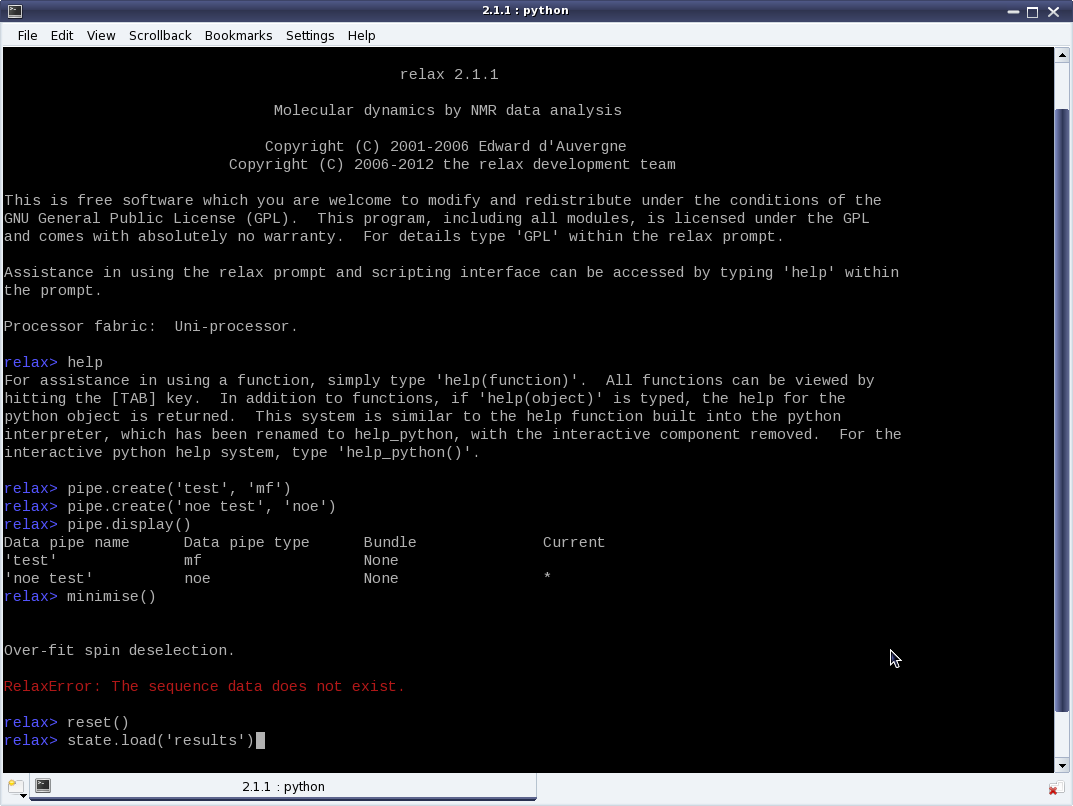
\includegraphics[width=0.9\textwidth, bb=14 14 1088 821]{graphics/screenshots/relax_prompt_mode}}
\caption[Prompt screenshot]{A screenshot of relax being run in the primary prompt mode.}\label{fig: relax prompt}
\end{figure}



% Python.
%~~~~~~~~

\subsection{Python}

\index{Python|textbf}
relax has been designed such that knowledge about Python is not required to be able to fully use the program.  A few basics though will aid in understanding relax.

A number of simple programming axioms includes that of strings\index{string}, integers\index{integer}, floating point numbers\index{floating point number}, and lists\index{list}.  A string is text and within Python (as well as relax) this is delimited by either single or double quotes.  An integer is a number with no decimal point whereas a float is a number with a decimal point.  A list in Python (called an array in other languages) is a list of anything separated by commas and delimited by square brackets, an example is \prompt{[0, 1, 2, `a', 1.2143235]}.

Probably the most important detail is that functions in Python require brackets around their arguments.  For example

\begin{lstlisting}[numbers=none]
relax> minimise()
\end{lstlisting}

will commence minimisation\index{optimisation} however

\begin{lstlisting}[numbers=none]
relax> minimise
\end{lstlisting}

will do nothing.

The arguments to a function are simply a comma separated list within the brackets of the function.  For example to save the program's current state type

\begin{lstlisting}[numbers=none]
relax> state.save('save', force=True)
\end{lstlisting}

Two types of arguments exist in Python\index{Python|textbf} -- standard arguments\index{argument} and keyword arguments\index{argument!keyword}.  The majority of arguments you will encounter within relax are keyword arguments however you may, in rare cases, encounter a non-keyword argument.  For these standard arguments just type the values in, although they must be in the correct order.  Keyword arguments consist of two parts -- the key and the value.  For example the key may be \prompt{file} and the value you would like to supply is \promptstring{R1.out}.  Various methods exist for supplying this argument.  Firstly you could simply type \promptstring{R1.out} into the correct position in the argument list.  Secondly you can type \prompt{file=`R1.out'}.  The power of this second option is that argument order is unimportant.  Therefore if you would like to change the default value of the very last argument, you don't have to supply values for all other arguments.  The only catch is that standard arguments must come before the keyword arguments.


% Script screenshot
\begin{figure}
\centerline{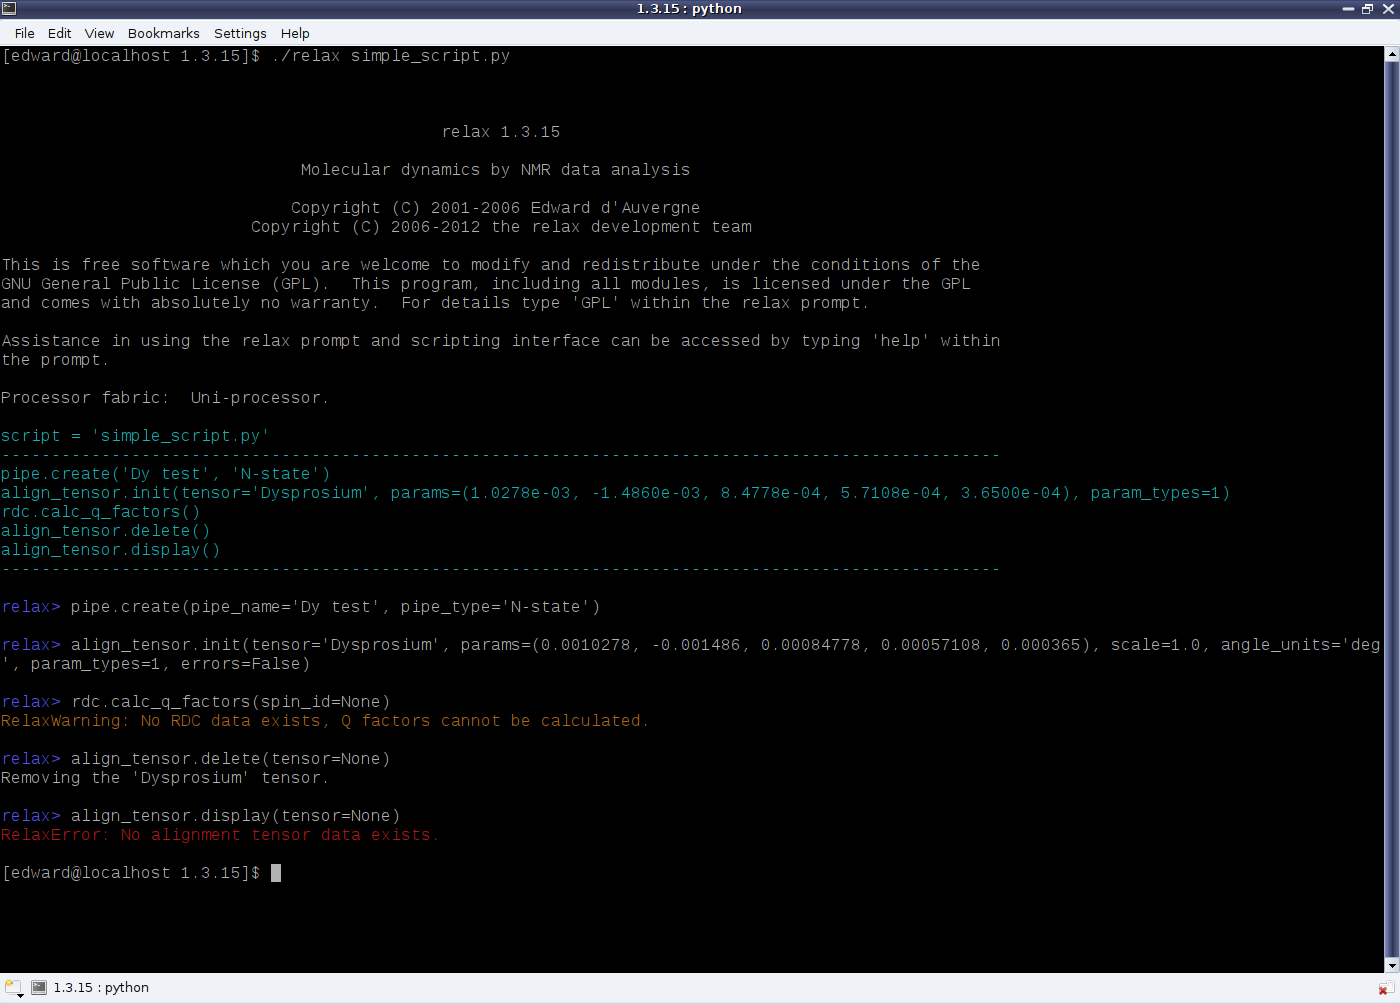
\includegraphics[width=0.9\textwidth, bb=14 14 1065 768]{graphics/screenshots/relax_script_mode}}
\caption[Scripting screenshot]{A screenshot of relax being run in scripting mode.}\label{fig: relax script}
\end{figure}


% User functions.
%~~~~~~~~~~~~~~~~

\subsection{User functions}
\index{user functions|textbf}

For standard data analysis a large number of specially tailored functions called ``user functions'' have been implemented.  These are accessible from the relax prompt by simply typing the name of the function.  An example is \uf{help()}\index{help system}.  An alphabetical listing of all accessible user functions together with full descriptions is presented later in this manual.

A few special objects which are available within the prompt are not actually functions.  These objects do not require brackets at their end for them to function.  For example to exit relax type

\begin{lstlisting}[numbers=none]
relax> exit
\end{lstlisting}

Another special object is that of the function class\index{function class}.  This object is simply a container which holds a number of user functions.  You can access the user function within the class by typing the name of the class, then a dot \promptstring{.}, followed by the name of the user function.  An example is the user function for reading relaxation data out of a file and loading the data into relax.  The function is called \promptstring{read} and the class is called \promptstring{relax\_data}.  To execute the function, type something like

\begin{lstlisting}[numbers=none]
relax> relax_data.read(ri_id='R1_600',  ri_type='R1',  frq=600.0*1e6, file='r1.600.out', res_num_col=1, data_col=3, error_col=4)
\end{lstlisting}

On first usage the relax prompt can be quite daunting.  Two features exist to increase the usability of the prompt -- the help system and tab completion.



% The help system.
%~~~~~~~~~~~~~~~~~

\subsection{The help system}
\index{help system|textbf}

For assistance in using a function simply type

\begin{lstlisting}[numbers=none]
relax> help(function)
\end{lstlisting}

In addition to functions if

\begin{lstlisting}[numbers=none]
relax> help(object)
\end{lstlisting}

is typed the help for the python object is returned.  This system is similar to the help function built into the python interpreter, which has been renamed to \prompt{help\_python}, with the interactive component removed.  For the standard interactive python help system type

\begin{lstlisting}[numbers=none]
relax> help_python()
\end{lstlisting}




% Tab completion.
%~~~~~~~~~~~~~~~~

\subsection{Tab completion}
\index{tab completion|textbf}

Tab completion is implemented to prevent insanity as the function names can be quite long -- a deliberate feature to improve usability.  The behaviour of the tab completion is very similar to that of the bash prompt.

Not only is tab completion useful for preventing RSI but it can also be used for listing all available functions.  To begin with if you hit the [TAB] key without typing any text all available functions will be listed (along with function classes\index{function class} and other python objects).  This extends to the exploration of user functions\index{user functions} within a function class\index{function class}.  For example to list the user functions within the function class \uf{model\_free} type

\begin{lstlisting}[numbers=none]
relax> model_free.
\end{lstlisting}

The dot character at the end is essential.  After hitting the [TAB] key you should see something like

\begin{lstlisting}[numbers=none]
relax| model_free.
model_free.__class__
model_free.__doc__
model_free.__init__
model_free.__module__
model_free.__relax__
model_free.__relax_help__
model_free.create_model
model_free.delete
model_free.remove_tm
model_free.select_model
relax> model_free.
\end{lstlisting}

All the objects beginning with an underscore are ``hidden'', they contain information about the function class\index{function class} and should be ignored.  From the listing the user functions\index{user functions} \uf{copy}, \uf{create\_model}, \uf{delete}, \uf{remove\_tm}, and \uf{select\_model} contained within \uf{model\_free} are all visible.

% GUI screenshot
\begin{figure}
\centerline{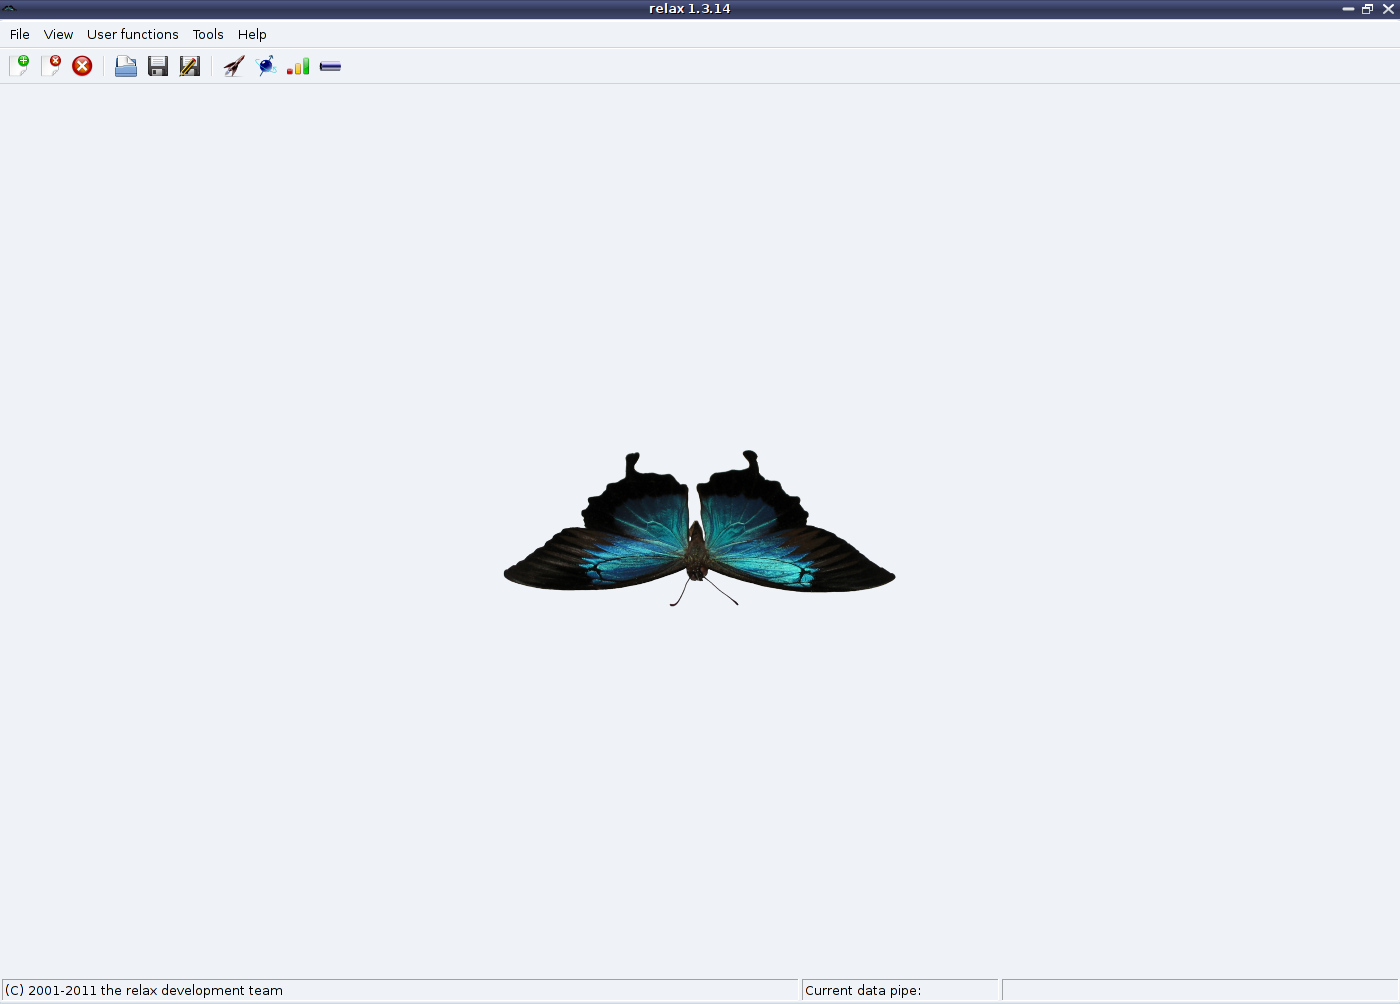
\includegraphics[width=0.9\textwidth, bb=14 14 1065 768]{graphics/screenshots/start}}
\caption[GUI screenshot]{Screenshot of the relax GUI interface -- the starting interface.  To start one of the automated analyses, either the menu \guimenuitemtwo{File}{New analysis} or the new analysis button in the toolbar should be selected.}\label{fig: GUI screenshot - start}
\end{figure}



% The data pipe.
%~~~~~~~~~~~~~~~

\subsection{The data pipe} \label{sect: the data pipe}
\index{data pipe|textbf}

Within relax all user functions operate on data stored within the current data pipe.  This pipe stores data is input, processed, or output as user functions are called.  There are different types of data pipe for different analyses, e.g. a reduced spectral density mapping pipe, a model-free pipe, an exponential curve-fitting pipe, etc.  Multiple data pipes can be created within relax and various operations performed in sequence on these pipes.  This is useful for operations such as model selection whereby the function \uf{model\_selection} can operate on a number of pipes corresponding to different models and then assign the results to a newly created pipe.  When running relax you choose which pipe you are currently in by using the \uf{pipe.switch} user function to jump between pipes. 

The flow of data through relax can be thought of as travelling through these pipes.  User functions\index{user functions} exist to transfer data between these pipes and other functions combine data from multiple pipes into one or vice versa.  The simplest invocation of relax would be the creation of a single data pipe and with the data being processed as it is passing through this pipe.

The primary method for creating a data pipe is through the user function\index{user functions} \uf{pipe.create}.  For example

\begin{lstlisting}[numbers=none]
relax> pipe.create('m1', 'mf')
\end{lstlisting}

will create a model-free data pipe labelled \promptstring{m1}.  The following is a table of all the types which can be assigned to a data pipe.

\begin{center}
\begin{tabular}{ll}
\toprule

Data pipe type          & Description \\

\midrule

\promptstring{ct}           & Consistency testing of relaxation data \\
\promptstring{frame order}  & The Frame Order analyses of domain motions \\
\promptstring{jw}           & Reduced spectral density mapping \\
\promptstring{hybrid}       & A special hybridised data pipe \\
\promptstring{mf}           & Model-free data analysis \\
\promptstring{N-state}      & N-state model of domain motions \\
\promptstring{noe}          & Steady state NOE calculation \\
\promptstring{relax\_fit}   & Relaxation curve-fitting \\

\bottomrule
\end{tabular}
\end{center}



% The spin and interatomic data containers.
%~~~~~~~~~~~~~~~~~~~~~~~~~~~~~~~~~~~~~~~~~~

\subsection{The spin and interatomic data containers}
\index{spin container|textbf}
\index{interatomic data container|textbf}

Any data which is not considered global for the molecule, such as diffusion tensors, alignment tensors, global minimisation statistics, etc., are stored within two special structures of the data pipes.  Any NMR data or information which is specific to an isolated spin system is stored within special spin containers.  This includes for example relaxation data, CSA information, nuclear isotope type, chemical element type, model-free parameters, reduced spectral density mapping values, spin specific minimisation statistics and PCS data.  NMR data or information which is defined as being between two spin systems, such as the magnetic dipole-dipole interaction involved in both NMR relaxation and RDC data, interatomic vectors and NOESY data, is stored within the interatomic data containers.  The spin and interatomic data containers and their associated data can be manipulated using a multitude of the relax user functions.


% Analysis wizard screenshot
\begin{figure}
\centerline{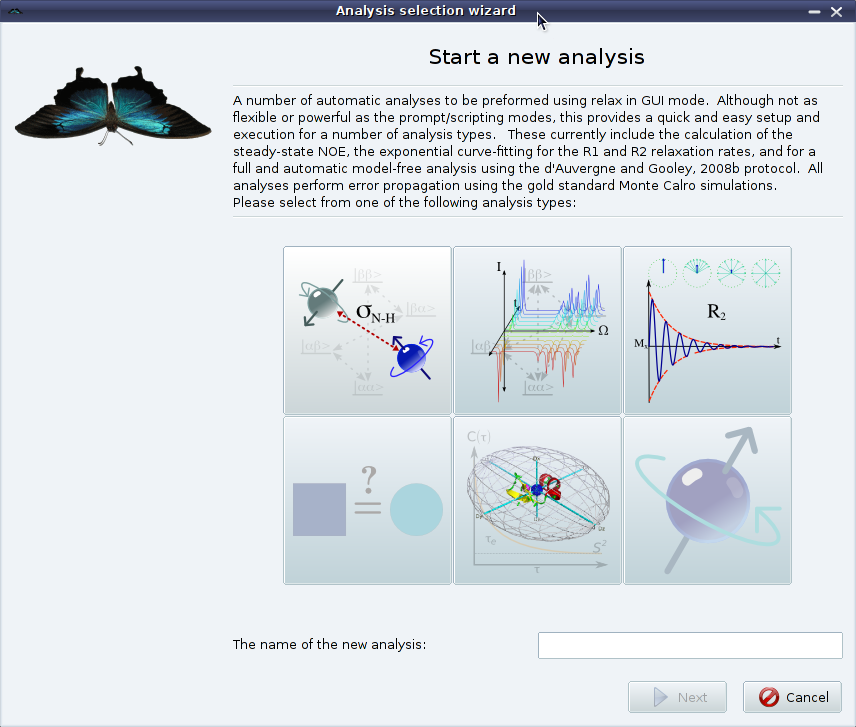
\includegraphics[width=0.7\textwidth, bb=14 14 657 560]{graphics/screenshots/analysis_wizard}}
\caption[GUI screenshot -- Analysis wizard screenshot]{Screenshot of the relax GUI interface -- the analysis selection wizard.  From here, the steady-state NOE analysis, the $\Rone$ and $\Rtwo$ relaxation rates via exponential curve-fitting, and the automated model-free analysis can be selected.}\label{fig: screenshot: analysis wizard}
\end{figure}



% Scripting.
%~~~~~~~~~~~

\subsection{Scripting} \label{sect: scripting}
\index{User interface!scripting|textbf}

What ever is done within the prompt is also accessible through scripting (Figure~\ref{fig: relax script}).  First type your commands into a text file ending in \file{*.py}.  To use this mode of relax, you will need to open up a terminal in your respective operating system:

\begin{description}
\item[GNU/Linux:]  Here you have an incredible number of choices.  If you don't have a preferred shell already, you could try one of \software{Konsole}, \software{GNOME Terminal} or even \software{XTerm} if you are a masochist.
\item[Mac OS X:]  This is as simple as in GNU/Linux -- just launch \software{Terminal.app} from the \directory{Utilities} folder.
\item[MS Windows:]  If your system supports it, you should install and use \software{Windows PowerShell}.  The alternative is the nasty \software{cmd} command line terminal program which comes installed by default on all Windows versions.  The \software{PowerShell}, although no where near as powerful as the Linux and Mac terminals, is a huge improvement on the ancient \software{cmd} program and will make relax much better to use on MS Windows.
\end{description}

Once your terminal is running, go to the directory containing your script using the \prompt{cd} command (if you do not know what this is, please see the documentation for your terminal program to understand some of its basic usage).  Once you are in the correct directory, within the terminal type:

\example{\$ relax your\_script.py}

You will need to replace \file{your\_script.py} with the name of your script.  In most cases you would probably like to keep a log of all of the messages, warnings and errors relax produces for future reference.  To active logging within relax, type:

\example{\$ relax --log log your\_script.py}

This will place all output (both STDOUT and STDERR) into the \file{log} file (you can choose any name for this log file).  Alternatively you can both log the output and simultaneously see the messages in your terminal by typing:

\example{\$ relax --tee log your\_script.py}

These command line arguments could be replaced by IO redirection if this is a familiar concept to you, but note that these arguments are active also in the GUI mode whereby IO redirection in the terminal will have no effect.   An example of a simple script which will minimise the model-free model ``m4'' after loading six relaxation data sets is

\begin{lstlisting}
# Create the data pipe.
name = 'm4'
pipe.create(name, 'mf')

# Load the PDB file.
structure.read_pdb('1f3y.pdb')

# Set up the 15N and 1H spins.
structure.load_spins('@N', ave_pos=True)
structure.load_spins('@H', ave_pos=True)
spin.isotope('15N', spin_id='@N')
spin.isotope('1H', spin_id='@H')

# Load the relaxation data.
relax_data.read(ri_id='R1_600',  ri_type='R1',  frq=600.0*1e6, file='r1.600.out', res_num_col=1, data_col=3, error_col=4)
relax_data.read(ri_id='R2_600',  ri_type='R2',  frq=600.0*1e6, file='r2.600.out', res_num_col=1, data_col=3, error_col=4)
relax_data.read(ri_id='NOE_600', ri_type='NOE', frq=600.0*1e6, file='noe.600.out', res_num_col=1, data_col=3, error_col=4)
relax_data.read(ri_id='R1_500',  ri_type='R1',  frq=500.0*1e6, file='r1.500.out', res_num_col=1, data_col=3, error_col=4)
relax_data.read(ri_id='R2_500',  ri_type='R2',  frq=500.0*1e6, file='r2.500.out', res_num_col=1, data_col=3, error_col=4)
relax_data.read(ri_id='NOE_500', ri_type='NOE', frq=500.0*1e6, file='noe.500.out', res_num_col=1, data_col=3, error_col=4)

# Initialise the diffusion tensor.
diffusion_tensor.init((2e-8, 1.3, 60, 290), param_types=1, axial_type='prolate', fixed=True)

# Create all attached protons.
sequence.attach_protons()

# Define the magnetic dipole-dipole relaxation interaction.
interatom.define(spin_id1='@N', spin_id2='@H', direct_bond=True)
interatom.set_dist(spin_id1='@N', spin_id2='@H', ave_dist=1.02 * 1e-10)
interatom.unit_vectors()

# Define the CSA relaxation interaction.
value.set(-172 * 1e-6, 'csa')

# Select a preset model-free model.
model_free.select_model(model=name)

# Grid search.
grid_search(inc=11)

# Minimise.
minimise('newton')

# Finish.
results.write(file='results', force=True)
state.save('save', force=True)
\end{lstlisting}

Scripting is much more powerful than the prompt as advanced Python\index{Python} programming can be employed (see the file \file{relax\_curve\_diff.py} in the \directory{sample\_scripts} directory for an example).



% Sample scripts.
\subsubsection{Sample scripts}
\index{scripting!sample scripts}

A few sample scripts have been provided in the directory \directory{sample\_scripts}.  These can be copied and modified for different types of data analysis.



% The test suite.
%~~~~~~~~~~~~~~~~

\subsection{The test suite}
\index{test suite}

To test that the program functions correctly, relax possesses an inbuilt test suite.  The suite is a collection of simple tests which execute or probe different parts of the program checking that the software runs without problem.  The test suite is executed by running relax using the command

\example{\$ relax --test-suite}

Alternatively the three components of the test suite -- system tests, unit tests, and GUI tests -- can be run separately with

\example{\$ relax --system-tests}

\example{\$ relax --unit-tests}

\example{\$ relax --gui-tests}


% NOE analysis screenshot
\begin{figure}
\centerline{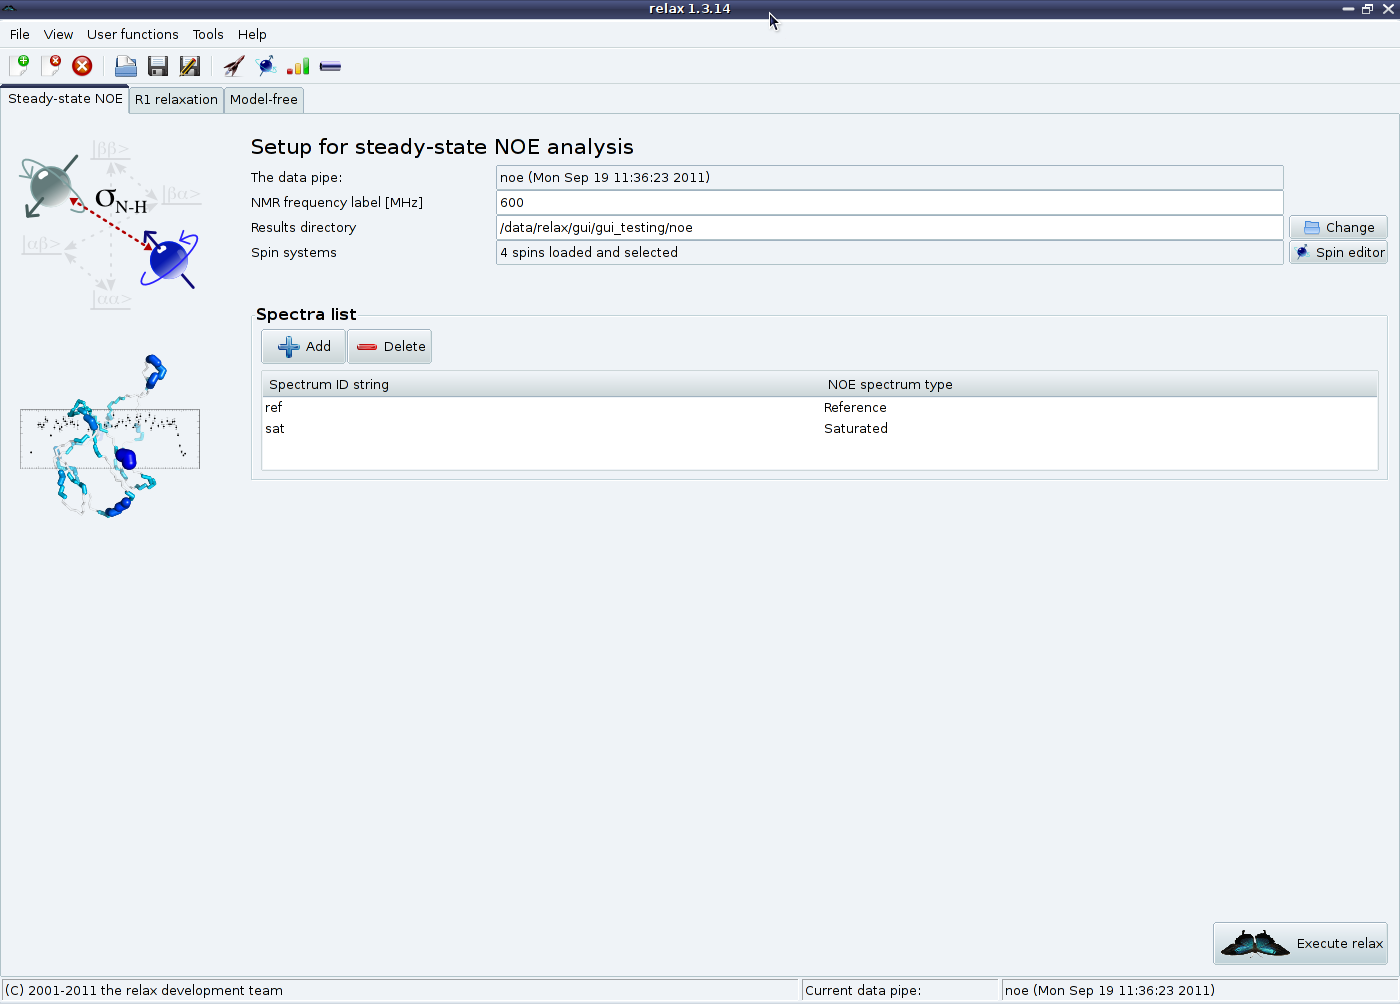
\includegraphics[width=\textwidth, bb=14 14 1065 768]{graphics/screenshots/analysis_noe}}
\caption[GUI screenshot -- NOE analysis]{Screenshot of the relax GUI interface -- the steady-state NOE analysis.}\label{fig: screenshot: NOE analysis}
\end{figure}


% The GUI.
%~~~~~~~~~

\subsection{The GUI}
\index{User interface!GUI|textbf}

% R1 analysis screenshot
\begin{figure}
\centerline{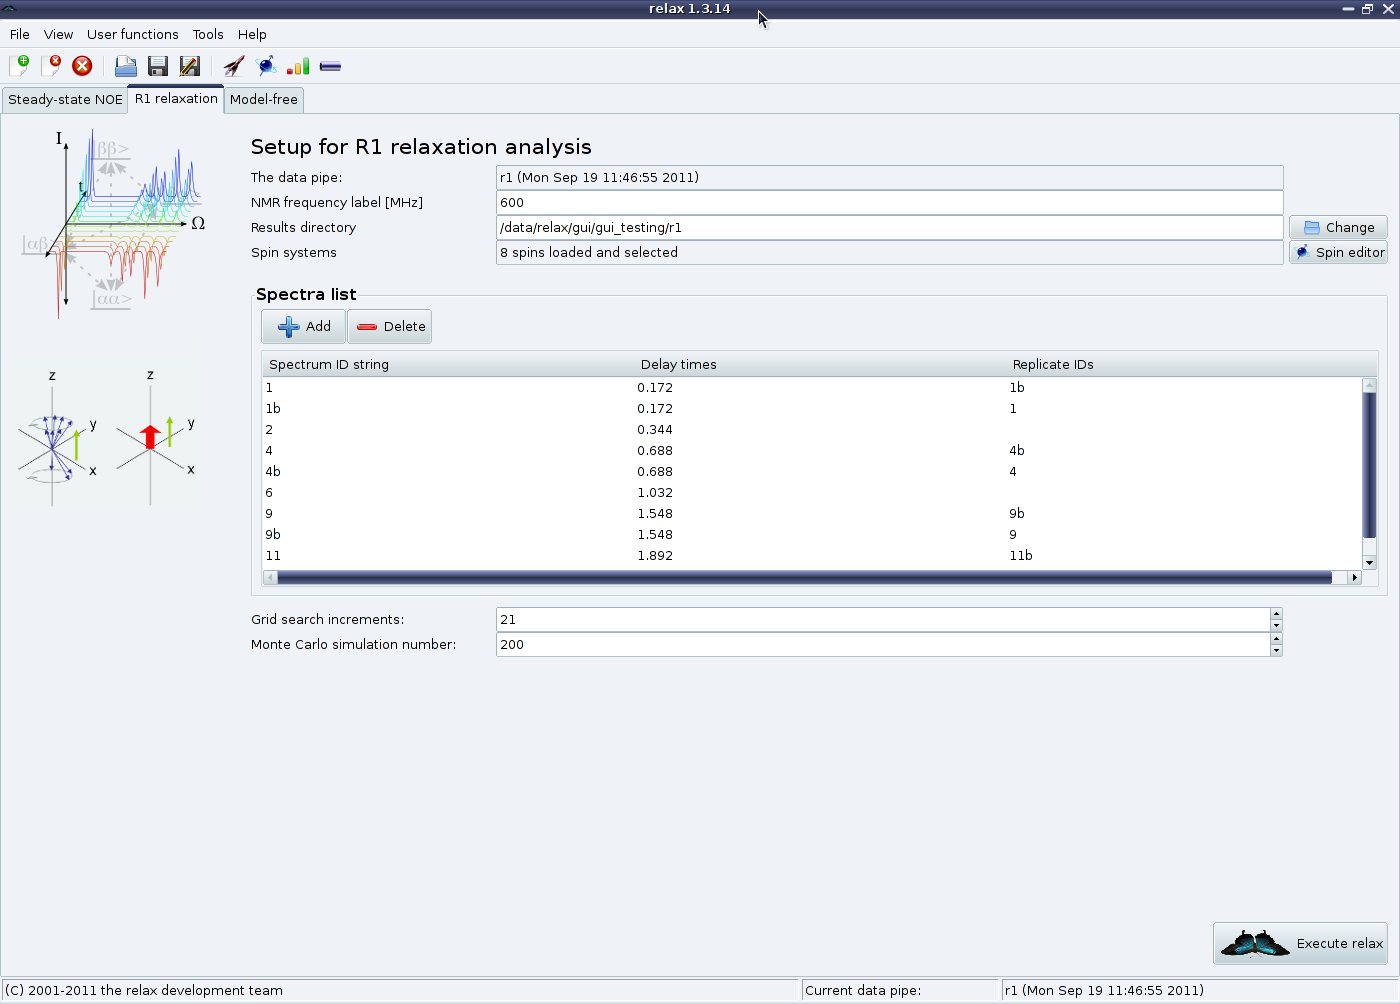
\includegraphics[width=\textwidth, bb=14 14 1065 768]{graphics/screenshots/analysis_r1}}
\caption[GUI screenshot -- $\Rone$ analysis]{Screenshot of the relax GUI interface -- the $\Rone$ analysis.}\label{fig: screenshot: R1 analysis}
\end{figure}


% R2 analysis screenshot
\begin{figure}
\centerline{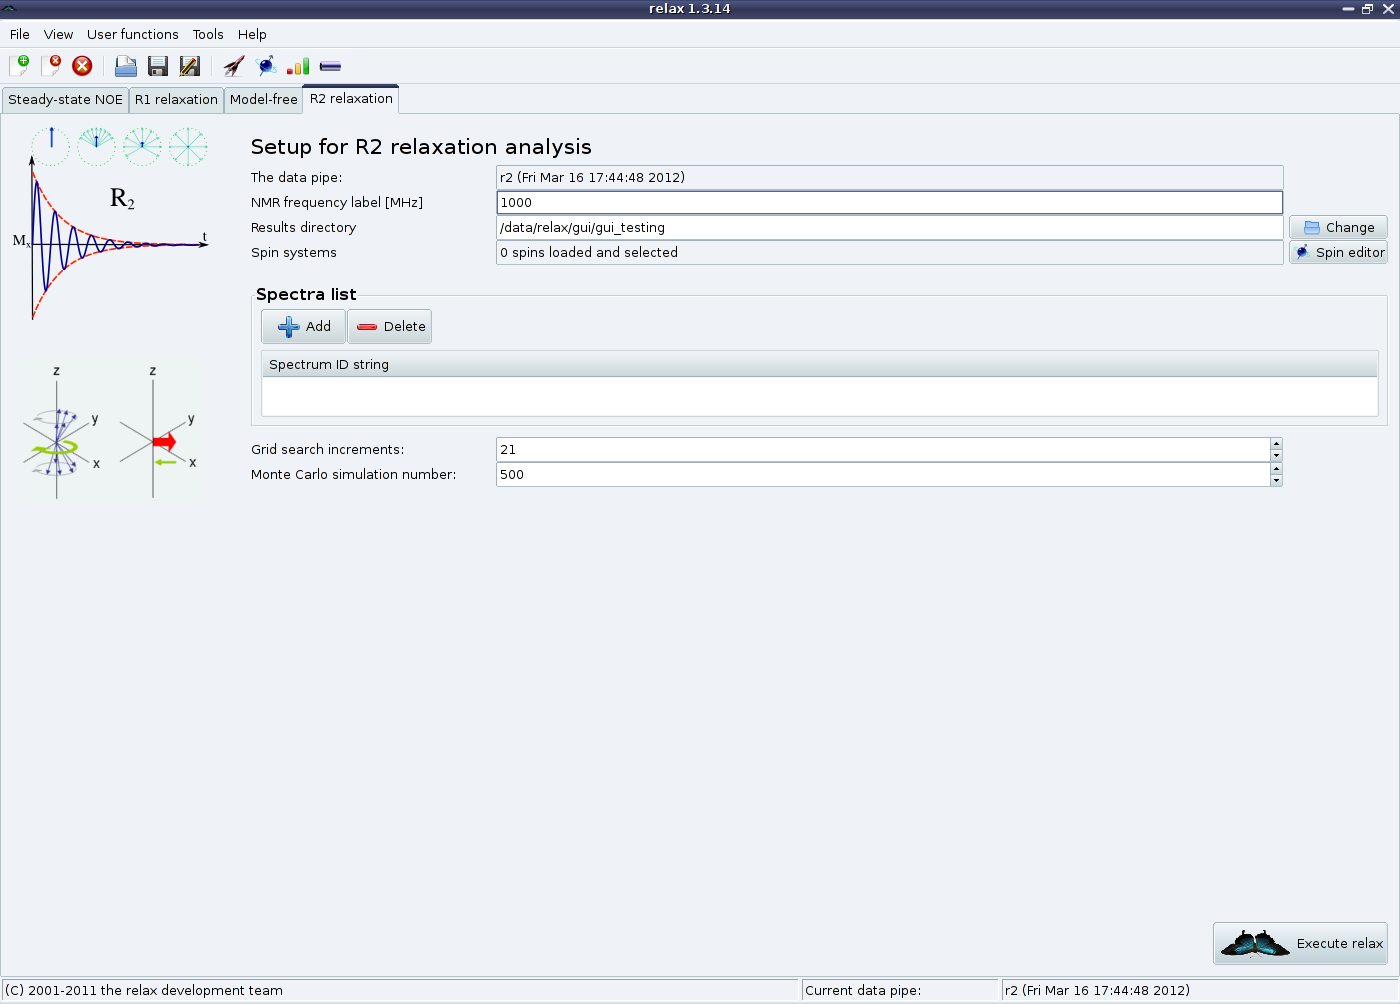
\includegraphics[width=\textwidth, bb=14 14 1065 768]{graphics/screenshots/analysis_r2}}
\caption[GUI screenshot -- $\Rtwo$ analysis]{Screenshot of the relax GUI interface -- the $\Rtwo$ analysis.}\label{fig: screenshot: R2 analysis}
\end{figure}

If the wxPython module is installed on your system, you will have access to the GUI interface of relax.  To launch relax in GUI mode, type either

\example{\$ relax -g}

or

\example{\$ relax --gui}

In most cases you will probably like to have a permanent copy of all the messages, warnings, and errors relax produces for future reference.  In such a case you could run the GUI with:

\example{\$ relax --gui --log log}

This will place all of the output into the \file{log} file.

% Model-free analysis screenshot
\begin{figure}
\centerline{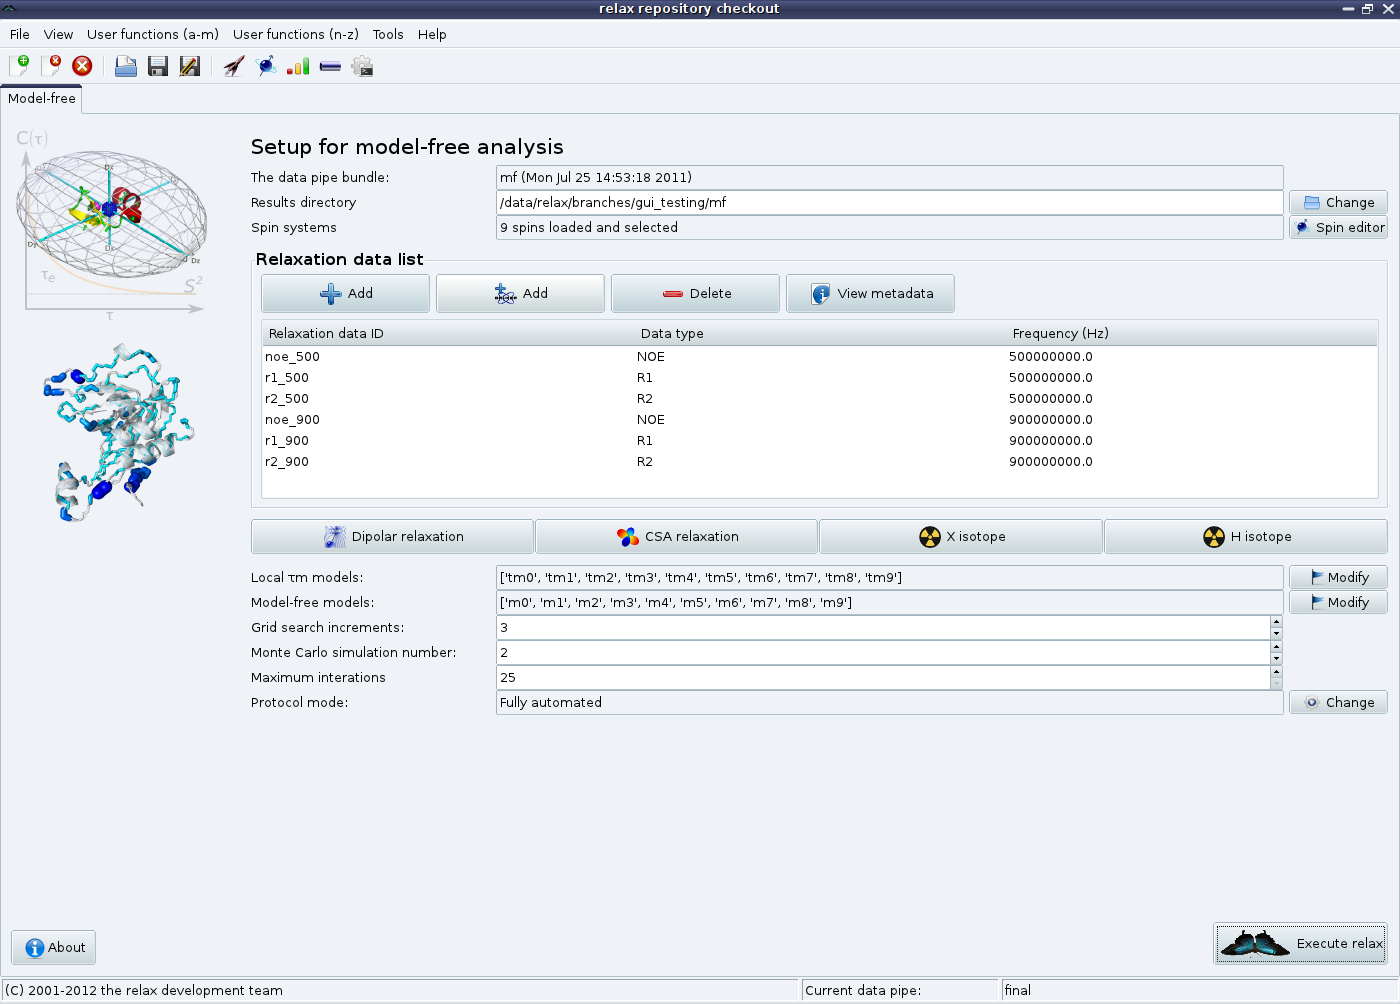
\includegraphics[width=\textwidth, bb=14 14 1065 768]{graphics/screenshots/analysis_mf}}
\caption[GUI screenshot -- Model-free analysis]{Screenshot of the relax GUI interface -- the automated model-free analysis.  The analysis is fully automated via a new model-free protocol as described in detail in Chapter~\ref{ch: model-free}.  Clicking on the \guibutton{About} button in the bottom left hand corner will give a full description of the protocol.  For using this interface or any of the modern-day model-free protocols, data from at least two magnetic field strengths must be without question collected.}\label{fig: screenshot: model-free analysis}
\end{figure}

The GUI is currently an interface to the automated analyses, providing an easy way to perform quick analyses.  The interface consists of a tab for each analysis.  By clicking on the \guimenuitemtwo{File}{New analysis} menu entry or the \guibutton{New analysis} toolbar button, the analysis wizard will appear (see Figure~\ref{fig: screenshot: analysis wizard}).  The following analyses can be set up using this wizard:

\begin{description}
\item[Steady-state NOE:]  this provides access to the steady-state NOE calculation with pseudo Monte Carlo simulations for error analysis (this falls back to bootstrapping as this is a calculation rather than optimisation).  See Figure~\ref{fig: screenshot: NOE analysis} on page~\pageref{fig: screenshot: NOE analysis}.
\item[$\Rone$ and $\Rtwo$]:  these provide easy access to optimisations and error analysis for the $\Rone$ and $\Rtwo$ relaxation rates via exponential curve-fitting (see Figures~\ref{fig: screenshot: R1 analysis} and~\ref{fig: screenshot: R2 analysis} on pages~\pageref{fig: screenshot: R1 analysis} and~\pageref{fig: screenshot: R2 analysis}).
\item[Model-free analysis]:  A fully automatic model-free protocol is provided in another tab.  This operates via the \module{dauvergne\_protocol} module which implements the protocol of \cite{dAuvergneGooley08b} (see Figure~\ref{fig: screenshot: model-free analysis} on page~\pageref{fig: screenshot: model-free analysis}).
\end{description}

A number of windows in the GUI provide user feedback or allow for the viewing and editing of data.  These include:

% relax controller screenshot
\begin{figure}
\centerline{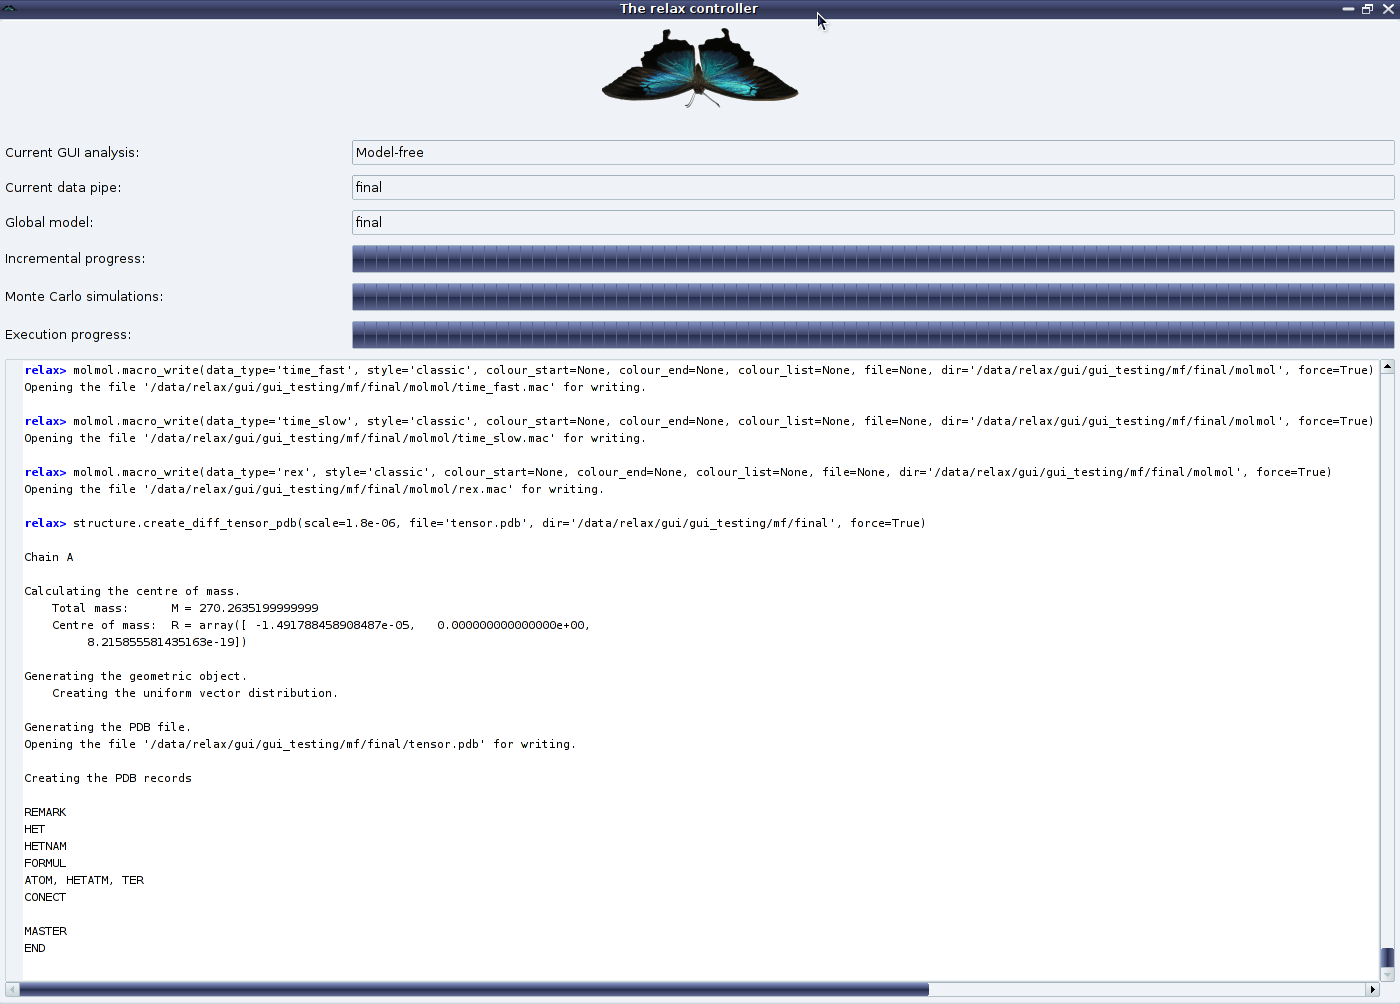
\includegraphics[width=0.9\textwidth, bb=14 14 1065 768]{graphics/screenshots/relax_controller}}
\caption[relax controller screenshot]{Screenshot of the relax GUI interface -- the relax controller window.  The purpose of the controller is for feedback.  It shows the current analysis and current data pipe, a number of progress gauges, and the relax text output.}\label{fig: screenshot: relax controller}
\end{figure}

% Spin viewer screenshot
\begin{figure}
\centerline{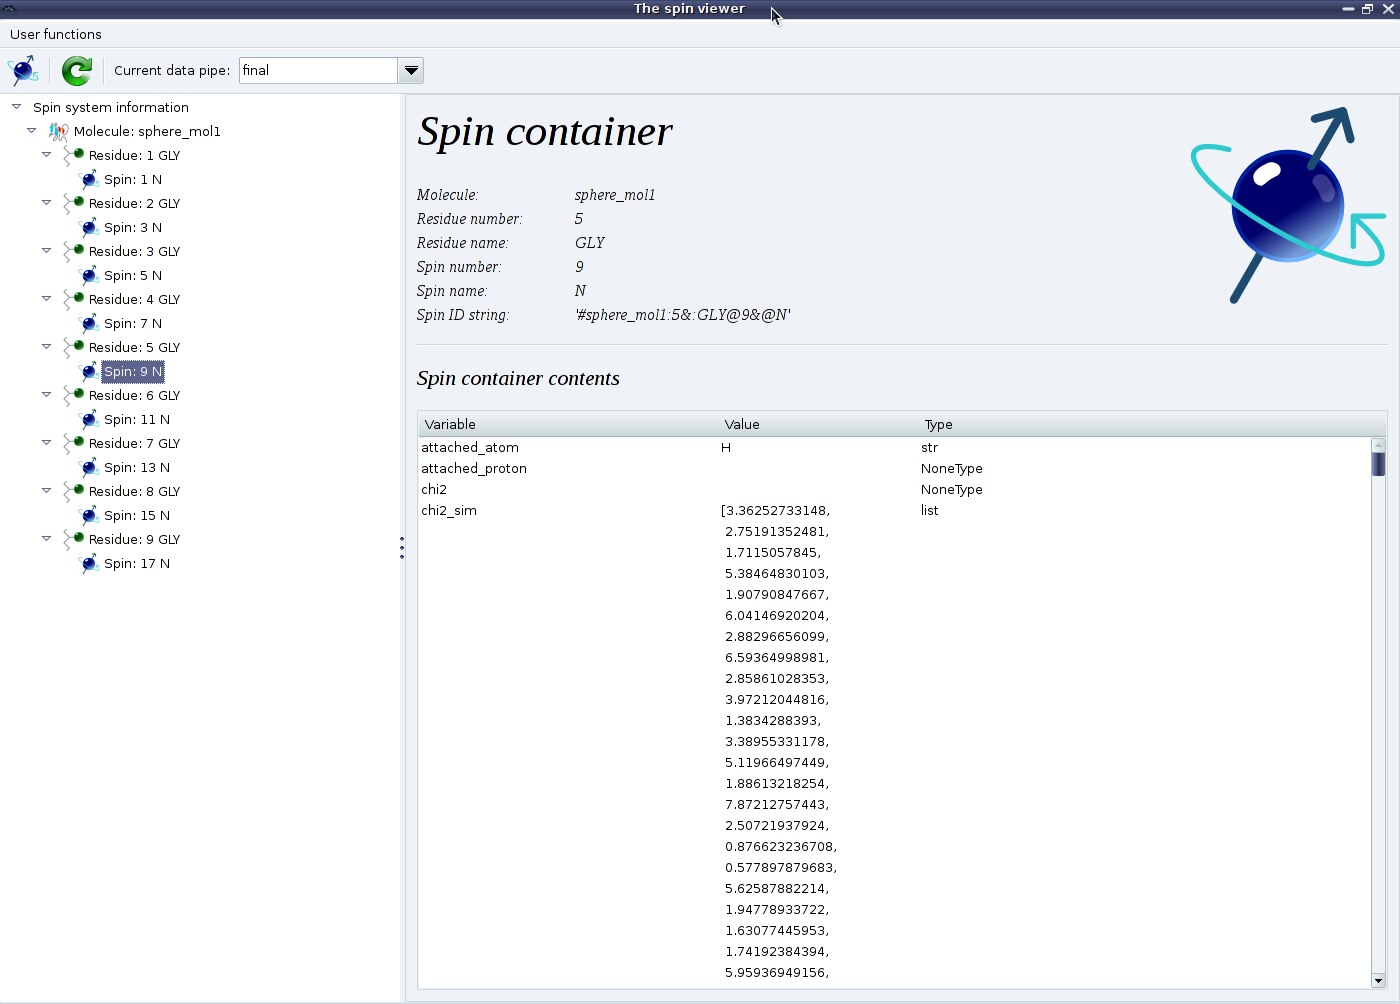
\includegraphics[width=0.9\textwidth, bb=14 14 1065 768]{graphics/screenshots/spin_viewer}}
\caption[Spin viewer window screenshot]{Screenshot of the relax GUI interface -- the spin viewer window.  This viewer is designed for easy addition and manipulation of spin systems within the relax data store.  The window is accessible via the \guimenuitemtwo{View}{Spin viewer} menu entry, typing \shortcutkey{Ctrl-T}, the spin viewer button in the toolbar, or the \guibutton{spin editor} button within the auto-analysis tabs.}\label{fig: screenshot: spin viewer}
\end{figure}

% Results viewer screenshot
\begin{figure}
\centerline{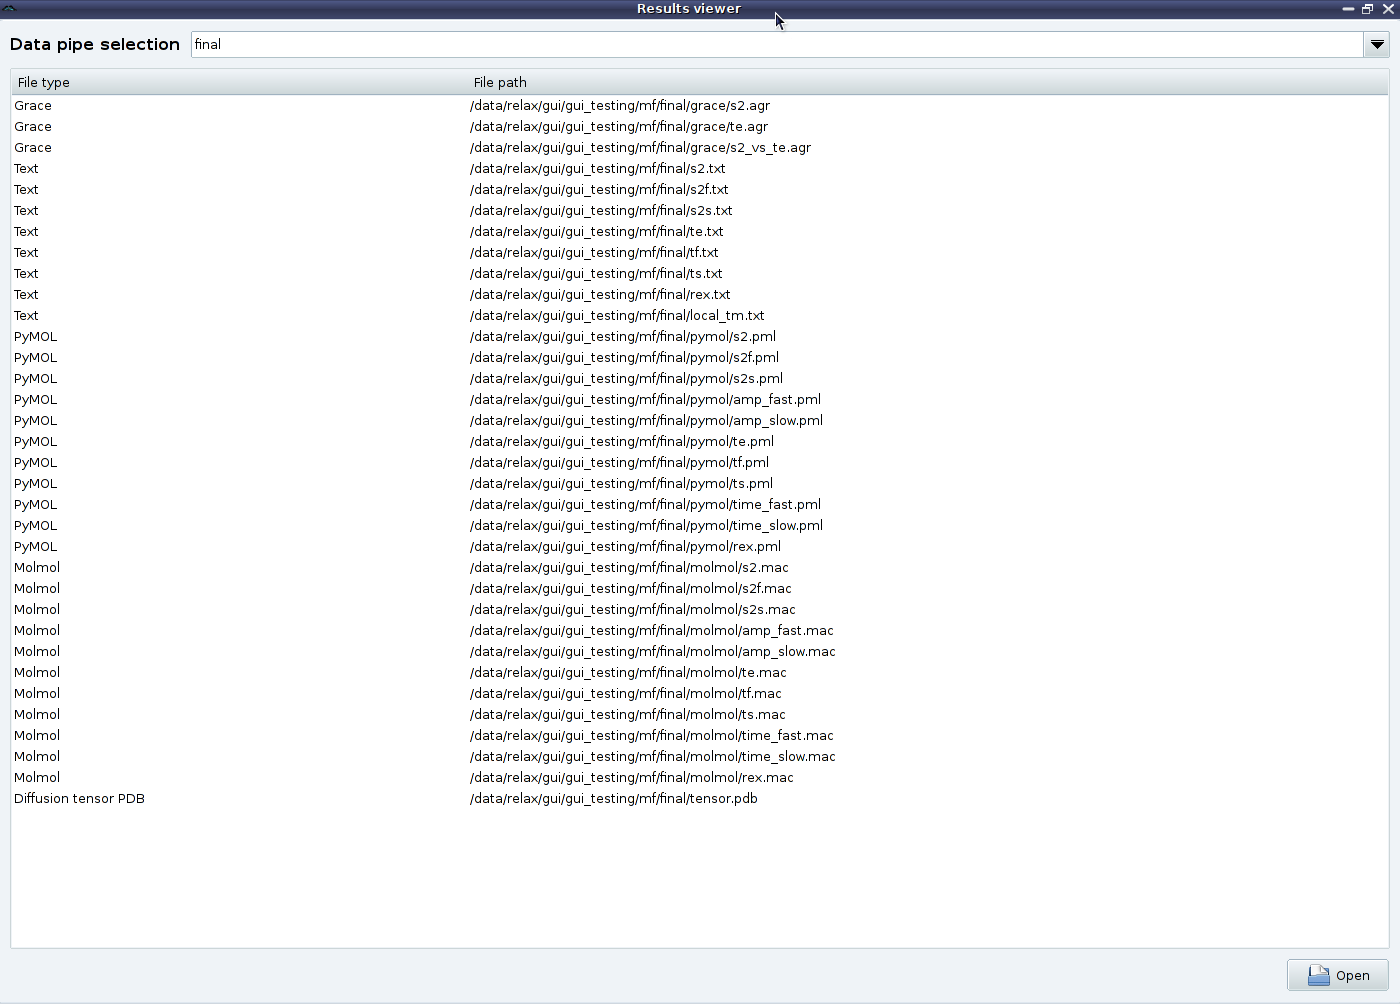
\includegraphics[width=0.9\textwidth, bb=14 14 1065 768]{graphics/screenshots/results_viewer}}
\caption[Results viewer window screenshot]{Screenshot of the relax GUI interface -- the results viewer window.  At the end of one of the automated analyses, a number of results files will be created.  This can include text files containing the results, 2D Grace plots of the results, PyMOL and MOLMOL macros plotting the results onto the structure, diffusion tensor objects for viewing in PyMOL, etc.  This window allows for easy opening of these results files.}\label{fig: screenshot: results viewer}
\end{figure}

% Pipe editor screenshot
\begin{figure}
\centerline{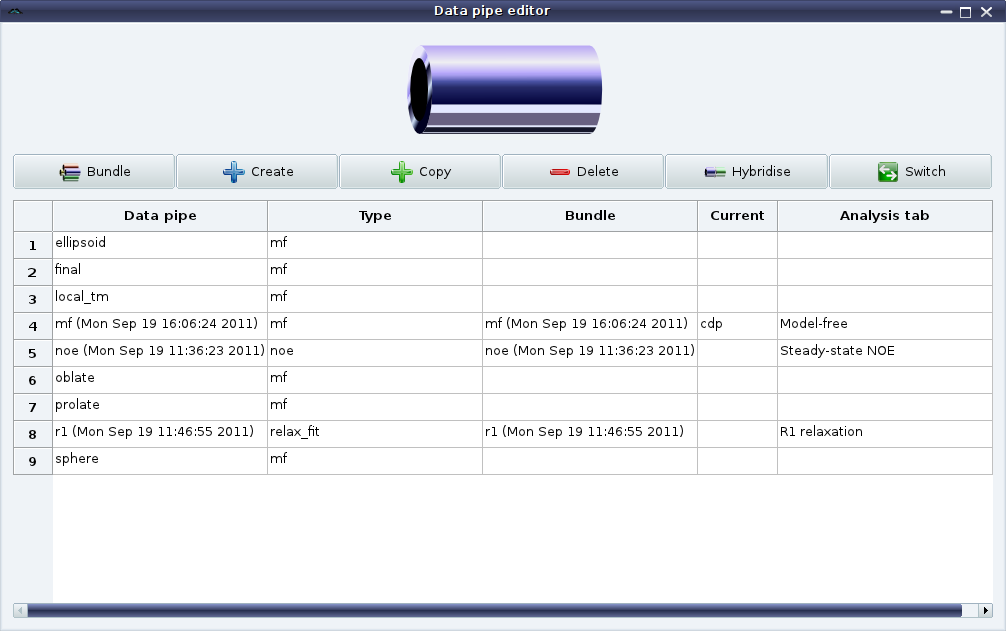
\includegraphics[width=0.9\textwidth, bb=14 14 769 488]{graphics/screenshots/pipe_editor}}
\caption[Pipe editor window screenshot]{Screenshot of the relax GUI interface -- the pipe editor window.  One analysis may consist of one or more data pipes.  And each analysis has its own unique set of data pipes.  This editor allows for the easy manipulation of data pipes for advanced users.}\label{fig: screenshot: pipe editor}
\end{figure}

% Prompt window screenshot
\begin{figure}
\centerline{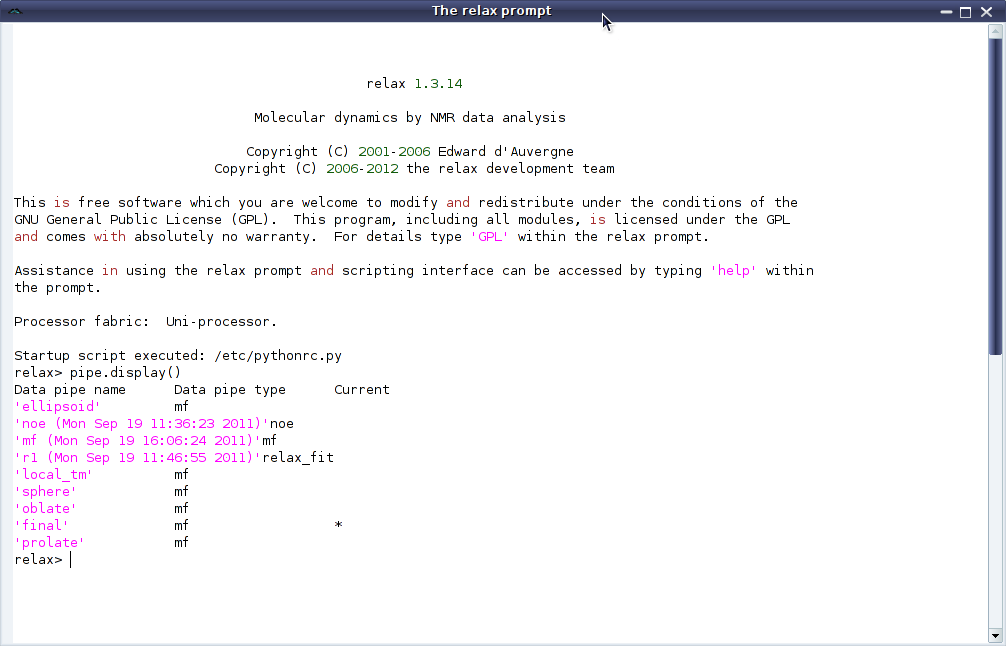
\includegraphics[width=0.8\textwidth, bb=14 14 769 499]{graphics/screenshots/relax_prompt}}
\caption[Prompt window screenshot]{Screenshot of the relax GUI interface -- the prompt window.  This window mimics relax in the prompt user interface mode, and provides the full power of the prompt/script UI modes within the GUI.}\label{fig: screenshot: prompt window}
\end{figure}


\begin{description}
\item[The relax controller]:  This window shows the progress of relax's execution and displays relax's text output for checking if the analysis has been performed correctly and has completed successfully (see Figure~\ref{fig: screenshot: relax controller}).
\item[Spin viewer window]:  This is used to load spins system information into the relax data store and to see the contents of the spin containers (see Figure~\ref{fig: screenshot: spin viewer}).
\item[Results viewer window]:  This presents a list of the results files which can be opened by double clicking for visualisation using a text editor, Grace, PyMOL, MOLMOL, etc (see Figure~\ref{fig: screenshot: results viewer}).
\item[Data pipe editor]:  This window allows for easy manipulation of the data pipes of the relax data store (see Figure~\ref{fig: screenshot: pipe editor}).
\item[The relax prompt]:  This window gives access to the relax prompt (see Figure~\ref{fig: screenshot: prompt window}).
\end{description}



% Access to the internals of relax.
%~~~~~~~~~~~~~~~~~~~~~~~~~~~~~~~~~~

\subsection{Access to the internals of relax}

To enable advanced Python\index{Python} scripting and control, many parts of relax have been designed in an object oriented fashion.  If you would like to play with internals of the program the entirety of relax is accessible by importation.  For example all data is contained within the object called the relax data store which, to be able to access it, needs be imported by typing:

\begin{lstlisting}[numbers=none]
relax> from data_store import Relax_data_store; ds = Relax_data_store()
\end{lstlisting}

The \prompt{ds} object is a dictionary type which contains the multiple data pipes.  All of relax's packages, modules, functions, and classes are also accessible by import statements.  For example to create a rotation matrix from three Euler angles in the z-y-z notation, type:

\begin{lstlisting}[numbers=none]
relax> alpha = 0.1342
relax> beta = 1.0134
relax> gamma = 2.4747
relax> from lib.geometry.rotations import euler_to_R_zyz
relax> from numpy import float64, zeros
relax> R = zeros((3,3), float64)
relax> euler_to_R_zyz(alpha, beta, gamma, R)
relax> print(R)
[[-0.494666415429033 -0.557373756841289 -0.666813041737502]
 [ 0.219125193028791 -0.822460914570202  0.524921131013452]
 [-0.84100492699311   0.113545317776532  0.528978424497956]]
relax>
\end{lstlisting}



% The multi-processor framework.
%%%%%%%%%%%%%%%%%%%%%%%%%%%%%%%%

\section{The multi-processor framework}
\index{multi-processor framework}



% Introduction.
%~~~~~~~~~~~~~~

\subsection{Introduction to the multi-processor} \label{sect: multi-processor}

Thanks to Gary Thompson's multi-processor framework, relax can be run on multi-core/multi-CPU systems or on clusters to speed up calculations.  As most analyses are relatively quick and would not benefit from the multi-processor framework, only the model-free and frame order analyses have currently been parallelised to run within this framework.  To use the multi-processor framework, the following should be installed:

\begin{description}
\item[\href{http://www.open-mpi.org/}{OpenMPI}\index{MPI!OpenMPI|textbf}:]  This is the most commonly used Message Passing Interface (MPI)\index{MPI} protocol software.  The rest of this manual will assume that this is the implementation in use.  If another implementation is used, please see the specific documentation for that software for how to set up a program to run via MPI.
\item[\href{http://mpi4py.scipy.org/}{mpi4py}\index{MPI!mpi4py|textbf}:]  This dependency is essential for running in MPI mode in relax.  If you would like to use another Python implementation to access the MPI protocol, please consider becoming a relax developer.
\end{description}



% Usage.
%~~~~~~~

\subsection{Usage of the multi-processor}

If you have access to a 256 node cluster and can run calculations on all nodes, assuming that the \file{dauvergne\_protocol.py} automated model-free analysis sample script will be used (after modification for the system under study), relax can be executed by typing:

\example{\$ mpirun -np 257 /usr/local/bin/relax --multi=`mpi4py' --tee log dauvergne\_protocol.py}

Note that the argument \prompt{-np} value is one more than the number of slaves you would like to run.  You should then see the following text in the initial relax printout:

\example{Processor fabric:  MPI 2.1 running via mpi4py with 256 slave processors \& 1 master.  Using Open MPI 1.4.3.}



% Further details.
%~~~~~~~~~~~~~~~~~

\subsection{Further details}

For a full description of the multi-processor framework and how to use it, please see Gary Thompson's official announcement on the \href{https://mail.gna.org/public/relax-devel/2007-05/msg00000.html}{relax-devel mailing list}.



% Usage of the name relax.
%%%%%%%%%%%%%%%%%%%%%%%%%%

\section{Usage of the name relax}

The program relax is so relaxed that the first letter should always be in lower case!

% Installation instructions.
%%%%%%%%%%%%%%%%%%%%%%%%%%%%

\chapter{Installation instructions}


% Dependencies.
%~~~~~~~~~~~~~~

\section{Dependencies}

The following packages need to be installed before using relax:
\begin{description}
  \item[\href{http://python.org/}{Python}\index{Python}:]  Version 2.5 or higher.
  \item[\href{http://numpy.scipy.org/}{NumPy}\index{NumPy}:]  Version 1.6 or higher.
    This package is used for most of the numerical calculations within relax.
  \item[\href{http://www.scipy.org/}{SciPy}\index{SciPy}:]  Version 0.7.1 or higher.
    This package is optional.
    It is required only for the frame order theory analyses.
  \item[\href{http://wxpython.org/}{wxPython}\index{wxPython}:]  Version 2.8 or higher.
    This package is also optional.
    It is required for the operation of the graphical user interface (GUI)\index{User interface!GUI}.
  \item[\href{http://mpi4py.scipy.org/}{mpi4py}\index{MPI!mpi4py}:]  Version 1.2 or higher.
    This optional dependency is essential for running relax in MPI multi-processor mode.
\end{description}

Older versions of these packages may work, use them at your own risk.
If, for older dependency versions, errors do occur please submit a bug report to the bug tracker\index{bug!tracker} at \href{https://gna.org/bugs/?group=relax}{https://gna.org/bugs/?group=relax}.
That way a solution may be created for the next relax release.

Note that only the official Python distribution from \href{http://python.org}{http://python.org} is supported.
If you use the Enthought Python Distribution (EPD) or other non-official distributions you may encounter problems with the relax C modules, the graphical user interface, or other issues.
These alternative distributions are to be used at your own risk.
Any issues encountered will not be considered as relax bugs.


% Installation.
%~~~~~~~~~~~~~~

\section{Installation}
\index{installation|textbf}


% The precompiled verses source distribution.
\subsection{The source releases}
\label{sect: source releases}

Two types of software packages are available for download -- the precompiled and source distribution.
Currently only relaxation curve-fitting requires compilation to function and all other features of relax will be fully functional without compilation.
If relaxation curve-fitting is required but no precompiled version of relax exists for your operating system or architecture then, if a C compiler is present, the C code can be compiled into the shared objects files \file{*.so}, \file{*.pyd} or \file{*.dylib} which are loaded as modules into relax\index{C module compilation}.
To build these modules the Scons\index{SCons|textbf} system from \href{http://scons.org/}{http://scons.org/} is required.
This software requires the Python and numpy header files installed.
Once Scons is installed type

\example{\$ scons}
\index{SCons|textbf}

in the base directory where relax has been installed and the C modules should, hopefully, compile without any problems.
Otherwise please submit a bug report to the bug tracker\index{bug!tracker} at \href{https://gna.org/bugs/?group=relax}{https://gna.org/bugs/?group=relax}.



% Installation on GNU/Linux.
\subsection{Installation on GNU/Linux}
\index{Operating system!GNU/Linux|textbf}

To install the program relax on a GNU/Linux system download either the precompiled distribution\index{distribution archive} labelled \file{relax-x.x.x.GNU-Linux.\textit{arch}.tar.bz2} matching your machine architecture or the source distribution \file{relax-x.x.x.src.tar.bz2}.
A number of installation methods are possible.
The simplest way is to switch to the user ``root'', unpack and decompress the archive within the \directory{\ossep{}usr\ossep{}local} directory by typing, for instance

\example{\$ tar jxvf relax-x.x.x.GNU-Linux.i686.tar.bz2}
\index{tar}

then create a symbolic link in \directory{\ossep{}usr\ossep{}local\ossep{}bin} by moving to that directory and typing

\example{\$ ln -s ../relax/relax .}
\index{symbolic link}

and finally possibly creating the byte-compiled Python \file{*.pyc} files to speed up the start time of relax by typing

\example{\$ python -m compileall .}

in the relax base directory.
Alternatively if the Scons system is installed, by typing as the root user

\example{\$ scons install}
\index{SCons!install|textbf}

in the relax base directory, a directory in \directory{\ossep{}usr\ossep{}local\ossep{}} called \file{relax} will be created, all the uncompressed and untarred files will be copied into this directory, a symbolic link in \directory{\ossep{}usr\ossep{}local\ossep{}bin} to the file \directory{\ossep{}usr\ossep{}local\ossep{}relax\ossep{}relax} will be created, and then finally the Python \file{*.pyc} files will be byte-compiled.
To change the installation path to a non-standard location the Scons script \file{sconstruct} in the base relax directory should be modified by changing the variable \prompt{INSTALL\osus{}PATH} to point to the desired location.



% Installation on MS Windows.
\subsection{Installation on MS Windows}
\index{Operating system!MS Windows|textbf}

In addition to the above dependencies, running relax on MS Windows requires a number of additional programs.
These include:
\begin{description}
  \item[\href{https://pypi.python.org/pypi/pyreadline}{pyreadline}\index{pyreadline}:]  Any version.
  \item[\href{http://starship.python.net/crew/theller/ctypes/}{ctypes}\index{ctypes}:]  The pyreadline package requires ctypes.
\end{description}

To install, simply download the pre-compiled binary distribution \file{relax-x.x.x.Win32.zip} or the source distribution \file{relax-x.x.x.src.zip} and extract the files to \directory{C:$\backslash$Program Files$\backslash$relax-x.x.x}.
Then add this directory to the system environment path (in Windows XP, right click on \gui{My Computer}, go to \gui{Properties}, click on the \gui{Advanced} tab, and click on the \guibutton{Environment Variables} button.
Then double click on the \gui{Path} system variable and add the text \guistring{;C:$\backslash$Program Files$\backslash$relax-x.x.x} to the end of variable value field.
The Python installation must also be located on the path (add the text \guistring{;C:$\backslash$Python27}, changing the text to point to the correct directory, to the field).
To run the program from any directory inside the Windows command prompt (or dos prompt) type:

\example{C:$\backslash$> relax}


Note that the pre-compiled binary distribution was built using a specific Python version and that that version may need to be installed for the modules to be loaded.
More details are given on the \href{http://www.nmr-relax.com/download.html}{download} webpage.


% Installation on Mac OS X.
\subsection{Installation on Mac OS X}
\index{Operating system!Mac OS X|textbf}

There are three ways of installing relax on a Mac.
These are described at \href{http://www.nmr-relax.com/download.html}{http://www.nmr-relax.com/download.html} and are the pre-compiled relax application, the Fink or the source releases.

\subsubsection{The relax application}

The stand-alone relax application requires none of the dependencies listed above to be installed.
It is a universal binary compiled for the i386, x86-64 and PPC CPU architectures (fat3) using the Mac OS X 10.5 framework.
It should therefore run on Leopard, Snow Leopard, and Lion.
This very large bundle does not require system administrator access to run.

\subsubsection{Fink}

Certain relax versions are available for Mac OS X within the Fink project.
These can be installed for Python 2.7 with the command:

\example{> fink install relax-py27}

The relax releases packaged within Fink can been browsed at \href{http://pdb.finkproject.org/pdb/browse.php?name=relax}{http://pdb.finkproject.org/pdb/browse.php?name=relax}.
If the desired version is not available, please download the relevant source package below or contact the fink project using the ``Maintainer'' email address given in the relax fink pages.

Note that when installing via fink, all the dependencies will be automatically selected and installed as well.
Although automatic, when starting from scratch that there could be well over 250 source packages that need to be compiled (to set up the full GNU compilation chain and other libraries which are then required to build Python, numpy, scipy, etc.).
This may take anywhere between 2 days to over a week (don't forget to mention this fact to your poor sys-admin).

The fink relax packages for different Python versions are \href{http://pdb.finkproject.org/pdb/package.php/relax-py27}{relax-py27}, \href{http://pdb.finkproject.org/pdb/package.php/relax-py26}{relax-py26}, \href{http://pdb.finkproject.org/pdb/package.php/relax-py25}{relax-py25} and \href{http://pdb.finkproject.org/pdb/package.php/relax-py24}{relax-py24}.

\subsubsection{Source release}

See Section~\ref{sect: source releases} on page~\pageref{sect: source releases}.


% Installation on your OS.
\subsection{Installation on your OS}

For all others systems, please use the source distribution files and the Scons software to build the C modules.



% Running a non-compiled version.
\subsection{Running a non-compiled version}

Compilation of the C code is not essential for running relax, however certain features of the program will be disabled.
Currently only the exponential curve-fitting for determining the $\Rone$ and $\Rtwo$ relaxation rates requires compilation.
To run relax without compilation install the dependencies detailed above, download the source distribution which should be named \file{relax-x.x.x.src.tar.bz2}, extract the files, and then run the file called \file{relax} in the base directory.



% Optional programs.
%~~~~~~~~~~~~~~~~~~~

\section{Optional programs}

The following is a list of programs which can be used by relax although they are not essential for normal use.


% Grace.
\subsection{Grace}
\index{software!Grace|textbf}

Grace is a program for plotting two dimensional data sets in a professional looking manner.
It is used to visualise parameter values.
It can be downloaded from \href{http://plasma-gate.weizmann.ac.il/Grace/}{http://plasma-gate.weizmann.ac.il/Grace/}.


% OpenDX.
\subsection{OpenDX}
\index{software!OpenDX|textbf}

Version 4.1.3 or compatible.
OpenDX is used for viewing the output of the space mapping function and is executed by passing the command \prompt{dx} to the command line with various options.
The program is designed for visualising multidimensional data and can be found at \href{http://www.opendx.org/}{http://www.opendx.org/}.


% Molmol.
\subsection{Molmol}
\index{software!MOLMOL|textbf}

Molmol is used for viewing the PDB structures loaded into the program and to display parameter values mapped onto the structure.


% PyMOL.
\subsection{PyMOL}
\index{software!PyMOL|textbf}

PDB structures can also be viewed using PyMOL.
This program can also be used to display geometric objects generated by relax for representing physical concepts such as the diffusion tensor and certain cone diffusion models.


% Dasha.
\subsection{Dasha}
\index{software!Dasha|textbf}

Dasha is a program used for model-free analysis of NMR relaxation data.
It can be used as an optimisation engine to replace the minimisation algorithms implemented within relax.


% Modelfree4.
\subsection{Modelfree4}
\index{software!Modelfree|textbf}

Art Palmer's Modelfree4 program is also designed for model-free analysis and can be used as an optimisation engine to replace relax's high precision minimisation algorithms.

% Open source infrastructure chapter.
%%%%%%%%%%%%%%%%%%%%%%%%%%%%%%%%%%%%%

\chapter{Open source infrastructure} \label{ch: open source}



% The relax web sites.
%~~~~~~~~~~~~~~~~~~~~~

\section{The relax web sites}
\index{web site|textbf}

The main web site for relax is \href{http://www.nmr-relax.com}{http://www.nmr-relax.com}.
From these pages general information about the program, links to the latest documentation, links to the most current software releases, and information about the mailing lists\index{mailing list} are available.
There are also Google\index{Google} search capabilities built into the pages for searching both the HTML version\index{manual!HTML} of the manual and the archives of the mailing lists\index{mailing list!archive}.

The relax web site is hosted by the Gna!\ project\index{Gna} (\href{https://gna.org/}{https://gna.org/}) which is described as ``a central point for development, distribution and maintenance of Libre Software (Free Software) projects''.
relax is a registered Gna!\ project and its primary Gna!\ web site is \href{https://gna.org/projects/relax}{https://gna.org/projects/relax}.
This site contains many more technical details than the main web site.



% The mailing lists.
%~~~~~~~~~~~~~~~~~~~

\section{The mailing lists}
\index{mailing list|textbf}

A number of mailing lists have been created covering different aspects of relax.
These include the announcement list\index{mailing list!relax-announce}, the relax users list\index{mailing list!relax-users}, the relax development list\index{mailing list!relax-devel}, and the relax committers list\index{mailing list!relax-commits}.


% relax-announce mailing list.
\subsection{relax-announce}

The relax announcement list ``relax-announce at gna.org''\index{mailing list!relax-announce} is reserved for important announcements about the program including the release of new program versions.
The amount of traffic on this list is relatively low.
If you would like to receive information about relax you can subscribe to the list by vising the information page at \href{https://mail.gna.org/listinfo/relax-announce/}{https://mail.gna.org/listinfo/relax-announce/}.
Previous announcements can be viewed at \href{https://mail.gna.org/public/relax-announce/}{https://mail.gna.org/public/relax-announce/}\index{mailing list!archive}.


% relax-users mailing list.
\subsection{relax-users}

If you would like to ask questions about relax, discuss certain features, receive help, or to communicate on any other subject related to relax the mailing list ``relax-users at gna.org''\index{mailing list!relax-users} is the place to post your message.
To subscribe to the list go to the relax-users information page at \href{https://mail.gna.org/listinfo/relax-users/}{https://mail.gna.org/listinfo/relax-users/}.
You can also browse the mailing list archives at \href{https://mail.gna.org/public/relax-users/}{https://mail.gna.org/public/relax-users/}\index{mailing list!archive}.


% relax-devel mailing list.
\subsection{relax-devel} \label{sect: relax-devel mailing list}

A second mailing list exists for posts relating to the development of relax.
The list is ``relax-devel at gna.org''\index{mailing list!relax-devel} and to subscribe go to the relax-devel information page at \href{https://mail.gna.org/listinfo/relax-devel/}{https://mail.gna.org/listinfo/relax-devel/}.
Feature requests, program design, or any other posts relating to relax's structure or code should be sent to this list instead.
The mailing list archives can be browsed at \href{https://mail.gna.org/public/relax-devel/}{https://mail.gna.org/public/relax-devel/}\index{mailing list!archive}.


% relax-commits mailing list.
\subsection{relax-commits}

One last mailing list is the relax commits list\index{mailing list!relax-commits}.
This list is reserved for automatically generated posts created by the version control software which looks after the relax source code and these web pages.
If you would like to become a developer you can subscribe to the list at relax-commits information page \href{https://mail.gna.oactuallyrg/listinfo/relax-commits/}{https://mail.gna.org/listinfo/relax-commits/}.
The list can also be browsed at \href{https://mail.gna.org/public/relax-commits/}{https://mail.gna.org/public/relax-commits/}\index{mailing list!archive}.


% Replying to a message.
\subsection{Replying to a message}

When replying to a message on these lists remember to hit `respond to all' so that the mailing list is included in the CC field.
Otherwise your message will only be sent to the original poster and not return back to the list.
Only messages to relax-users and relax-devel will be accepted.
If you are using Gmail's web based interface, please do not click on `Edit Subject' as this currently mangles the email headers, creates a new thread on the mailing list, and makes it difficult to follow the thread.



% Reporting bugs.
%~~~~~~~~~~~~~~~~

\section{Reporting bugs}\label{reporting bugs}
\index{bug|textbf}

One of the philosophies in the construction of relax is that if there is something which is not immediately obvious then that is considered a design bug\index{bug!design}.
If any flaws in relax are uncovered including general design flaws, bugs in the code, or documentation issues these can be reported within relax's bug tracker system\index{bug!tracker}.
The link to submit a bug is \href{https://gna.org/bugs/?group=relax\&func=additem}{https://gna.org/bugs/?group=relax\&func=additem} while the main page for browsing, submitting, viewing the statistics, or searching through the database is at \href{https://gna.org/bugs/?group=relax}{https://gna.org/bugs/?group=relax}.
Please do not report bugs to personal email addresses or to the mailing lists.

When reporting a bug please include as much information as possible so that the problem can be reproduced.
Include information such as the release version or the revision number if the repository sources are being used.
Also include all the steps performed in order to trigger the bug.
Attachment of files is allowed so scripts and subsets of the input data can be included.
However please do not attach large files to the report.
Prior to reporting the bug try to make sure that the problem is indeed a bug and if you have any doubts please feel free to ask on the relax-users mailing list\index{mailing list!relax-users}.
To avoid duplicates be sure that the bug has not already been submitted to the bug tracker\index{bug!tracker}.
You can search the bugs\index{bug!search} from the page \href{https://gna.org/project/search.php?group=relax}{https://gna.org/project/search.php?group=relax}.

Once the bug has been confirmed by one of the relax developers you may speed up the resolution of the problem by trying to fixing the bug yourself.
If you do wish to play with the source code and try to fix the issue see the relax development chapter of this manual on how to check out the latest sources (Chapter~\ref{ch: relax devel} on page~\pageref{ch: relax devel}), how to generate a patch (which is just the output of diff\index{diff} in the `unified' format), and the guidelines for the format of the code.



% Latest sources -- the relax repositories.
%~~~~~~~~~~~~~~~~~~~~~~~~~~~~~~~~~~~~~~~~~~

\section{Latest sources -- the relax repositories}
\index{repository|textbf}

relax's source code is kept within a version control system called Subversion\index{Subversion|textbf} (\href{http://subversion.tigris.org/}{http://subversion.tigris.org/}).
Subversion or SVN\index{SVN|textbf} allows fine control over the development of the program.
The repository contains all information about every change ever made to the program.
To learn more about the system the Subversion book\index{Subversion!book} located at \href{http://svnbook.red-bean.com/}{http://svnbook.red-bean.com/} is a good place to start.
The contents of the relax repository can be viewed on-line at \href{http://svn.gna.org/viewcvs/relax/}{http://svn.gna.org/viewcvs/relax/}.
The current sources can be downloaded using the SVN protocol by typing

\example{\$ svn co svn://svn.gna.org/svn/relax/trunk relax-trunk}
\index{Subversion!check out}

however if this does not work, try the command

\example{\$ svn co http://svn.gna.org/svn/relax/trunk relax-trunk}
\index{Subversion!check out}

to download using the HTTP protocol.
The entire relax repository is backed up daily to \href{http://svn.gna.org/daily/relax.dump.gz}{http://svn.gna.org/daily/relax.dump.gz}\index{repository!back up}.



% News.
%~~~~~~

\section{News}
\index{news|textbf}

Summaries of the latest news on relax can be found on the relax web site \href{https://gna.org/projects/relax}{https://gna.org/projects/relax}.
However more information can be found at the dedicated news page \href{https://gna.org/news/?group=relax}{https://gna.org/news/?group=relax}.



% The relax distribution archives.
%~~~~~~~~~~~~~~~~~~~~~~~~~~~~~~~~~

\section{The relax distribution archives}
\index{distribution archive}

The relax distribution archives, the files to download to install relax, can be found at \href{http://download.gna.org/relax/}{http://download.gna.org/relax/}.
If a compiled binary distribution for your architecture does not exist you are welcome to create this distribution yourself and submit it for inclusion in the relax project.
To do this a number of steps are required.
Firstly, the code to each relax release or version resides in the `tags' directory of the relax repository.
To check out version 2.1.1 for example type

\example{\$ svn co svn://svn.gna.org/svn/relax/tags/2.1.1 relax}
\index{Subversion!check out}

Again the sources are available through HTTP by typing

\example{\$ svn co http://svn.gna.org/svn/relax/tags/2.1.1 relax}
\index{Subversion!check out}

The binary distribution can then be created for your architecture by shifting to the main directory of the checked out sources and typing

\begin{exampleenv}
\$ cd relax \\
\$ scons binary\_dist
\end{exampleenv}
\index{SCons!binary distribution}

At the end SCons\index{SCons} will attempt to make a GPG signature\index{GPG!signature} for the newly created archive.
However this will fail as the current relax private GPG key\index{GPG!key} is not available for security reasons.
If the SCons command fails, excluding the GPG signing, please submit a bug report\index{bug!tracker} with as much information possible including the details described next to \href{https://gna.org/bugs/?group=relax\&func=additem}{https://gna.org/bugs/?group=relax\&func=additem} (the python and SCons version numbers may also be useful).
Once the file has been created post a message to the relax development mailing list\index{mailing list!relax-devel} describing the compilation and the creation of the archive, the relax version number, the machine architecture, operating system, and the name of the new file.
Do not attach the file though.
You will then receive a response explaining where to send the file to.
For security the archive will be thoroughly checked and if the source code is identical to that in the repository and the C modules are okay, the file will be GPG signed\index{GPG!signature} and uploaded to \href{http://download.gna.org/relax/}{http://download.gna.org/relax/}.

% The relax data model.
%%%%%%%%%%%%%%%%%%%%%%%

\chapter{The relax data model} \label{ch: data model}


% Introduction.
%%%%%%%%%%%%%%%

\section{The concept of the relax data model}

To begin to understand how to use relax, a basic comprehension of the relax data model is needed.
The data model includes the concepts of the relax data store, the data pipes, the molecule, residue and spin data structures and the interatomic data containers.
These concepts are independent of the specific analyses presented in the next chapters and are important for setting up relax.



% The data model.
%%%%%%%%%%%%%%%%%

\section{The data model}


% The relax data store.
%~~~~~~~~~~~~~~~~~~~~~~

\subsection{The relax data store}

All permanent data handled by relax is kept in a structure known as the relax data store.
This structure is initialised when relax is launched.
The data store is primarily organised into a series of objects known as data pipes, and all usage of relax revolves around the flow of information in these data pipes.


% Data pipes.
\subsubsection{Data pipes}

\begin{figure*}[h]
  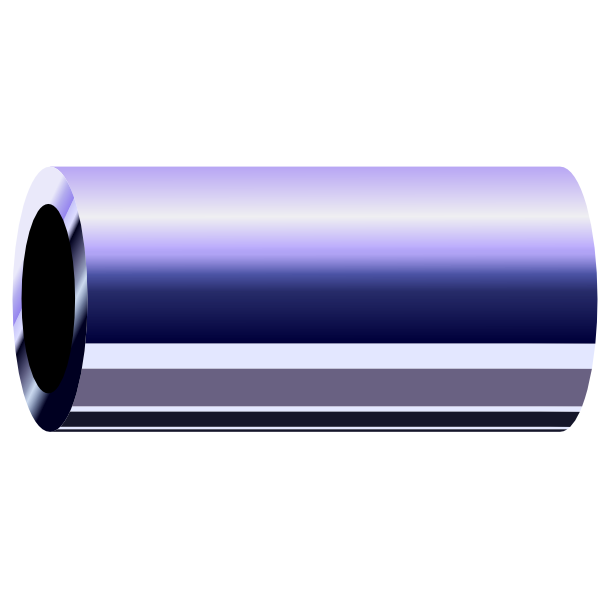
\includegraphics[width=3cm, bb=0 0 1701 1701]{graphics/misc/pipe_600x600}
\end{figure*}

The first thing one must do when relax is launched is to create a data pipe.
When using the GUI, a base data pipe will be created when opening one of the automatic analyses via the analysis selection window (see figure~\ref{fig: screenshot: analysis wizard} on page~\pageref{fig: screenshot: analysis wizard}).
This will also create a data pipe bundle for the analysis (\textit{vide infra}).
Alternatively the data pipe editor window can be used to create data pipes (see figure~\ref{fig: screenshot: pipe editor} on page~\pageref{fig: screenshot: pipe editor}).
For the prompt/scripting modes, or the \guimenuitemthree{User functions}{pipe}{create} menu entry, a data pipe can be initialised by specifying the unique name of the data pipe and the data pipe type:

\begin{lstlisting}
pipe.create(pipe_name='NOE 1200 MHz', pipe_type='noe')
\end{lstlisting}

A number of relax operations will also create data pipes by merging a group of pipes or branching pre-existing pipes.
See section~\ref{sect: the data pipe} on page~\pageref{sect: the data pipe} for additional details.

All data not associated with spin systems will be stored in the base data pipe.
This includes information such as global optimisation statistics, diffusion tensors, alignment tensors, 3D structural data, the molecule, residue and spin container data structure and the interatomic data containers.
One data pipe from the set will be defined as being the current data pipe, and all operations in relax will effect data from this pipe.
The \uf{pipe\ufsep{}switch} user function in all UI modes can be used to change which pipe is the current data pipe.
In the GUI, switching between analysis tabs will automatically switch the current data pipe to match the analysis being displayed.


% Data pipe bundles.
\subsubsection{Data pipe bundles} \label{sect: data pipe bundles}

\begin{figure*}[h]
  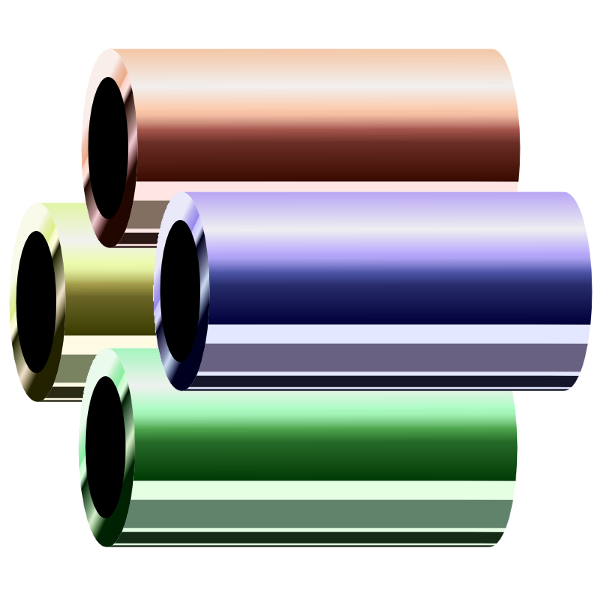
\includegraphics[width=3cm, bb=0 0 1701 1701]{graphics/misc/pipe_bundle_600x600}
\end{figure*}

Related data pipes can be grouped into a `bundle'.
For example if the data pipes ``sphere'', ``oblate spheroid'', ``prolate spheroid'', and ``ellipsoid'' preexist, these can be grouped into a bundle called ``diffusion tensors'' with the following series of user function calls:

\begin{lstlisting}
pipe.bundle(bundle='diffusion tensors', pipe='sphere')
pipe.bundle(bundle='diffusion tensors', pipe='oblate spheroid')
pipe.bundle(bundle='diffusion tensors', pipe='prolate spheroid')
pipe.bundle(bundle='diffusion tensors', pipe='ellipsoid')
\end{lstlisting}

The data pipe editor window of the GUI can also be used to bundle pipes together (see figure~\ref{fig: screenshot: pipe editor} on page~\pageref{fig: screenshot: pipe editor}).



% Molecule, residue, and spin containers.
%~~~~~~~~~~~~~~~~~~~~~~~~~~~~~~~~~~~~~~~~

\subsection{Molecule, residue, and spin containers}

Within a data pipe is the molecule, residue, and spin container data structure.
Data which is specific to a given nucleus is stored in a special spin container structure.
This includes relaxation data, model-free parameters, reduced spectral density mapping values, spin specific optimisation parameters, chemical shift tensor information, pseudo-contact shift values, etc.
The spin containers can be created from 3D structural data or a sequence file, as described in the next two sections, or manually built.



% Molecule containers.
\subsubsection{Molecule containers}

\begin{figure*}[h]
  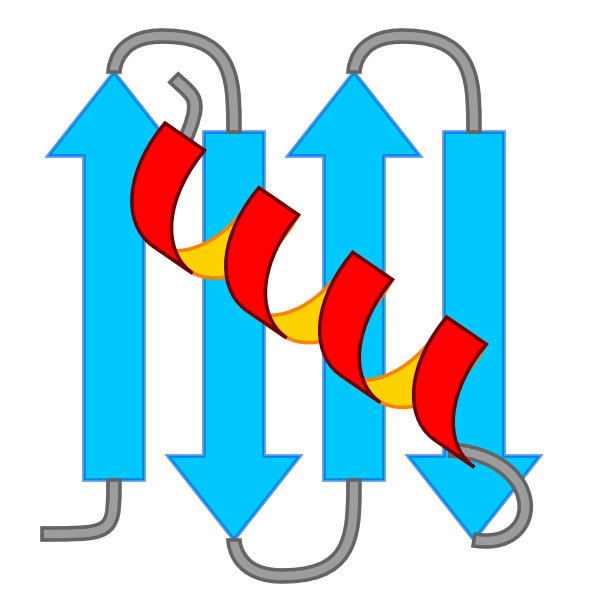
\includegraphics[width=3cm, bb=0 0 1701 1701]{graphics/misc/molecule_600x600}
\end{figure*}

The spin containers are part of a nested set of containers, and are graphically depicted in the spin viewer window of the GUI in figure~\ref{fig: screenshot: spin viewer} on page~\pageref{fig: screenshot: spin viewer}.
As can be seen from the figure, the top level holds a single molecular container.
Multiple molecular containers can be present if the study is of a molecular complex.
Using the GUI menus or the prompt/scripting mode, molecule containers can be manually created with the user function:

\begin{lstlisting}
molecule.create(mol_name='glycerol', mol_type='organic molecule')
\end{lstlisting}

In the spin viewer window of the GUI, right clicking on the \gui{Spin system information} element will pop up a menu with an entry for adding molecule containers.
Right clicking on molecule containers will show a pop up menu with an entry for permanently deleting the container.



% Residue containers.
\subsubsection{Residue containers}

\begin{figure*}[h]
  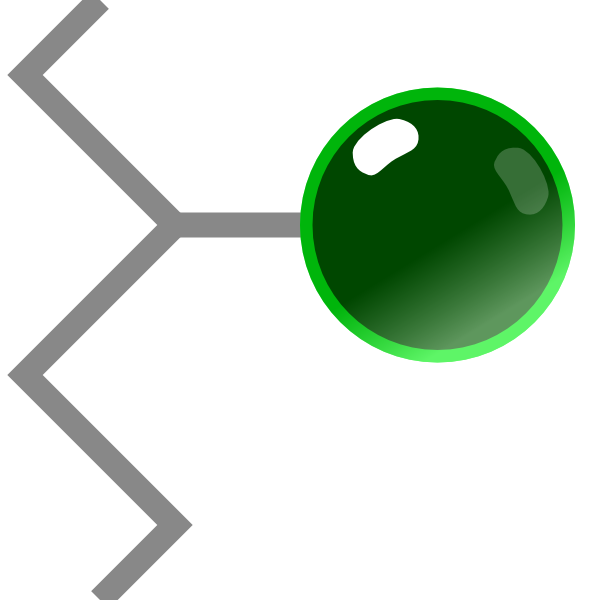
\includegraphics[width=3cm, bb=0 0 1701 1701]{graphics/misc/residue_600x600}
\end{figure*}

Nested within the molecule containers are residue containers.
These are graphically depicted in the spin viewer window (see figure~\ref{fig: screenshot: spin viewer} on page~\pageref{fig: screenshot: spin viewer}).
Each molecule container can possess multiple residues.
These require either a unique residue number or unique residue name.
For organic molecules where the residue concept is meaningless, all spin containers can be held within a single unnamed and unnumbered residue container.
Using the GUI menus or the prompt/scripting mode, residue containers can be manually created with the user function:

\begin{lstlisting}
residue.create(res_num='-5', res_name='ASP')
\end{lstlisting}

Alternatively residues can be added in the spin viewer window from the pop up menu when right clicking on molecule containers, and can be deleted via the pop up menu when right clicking on the residue to delete.



% Spin containers.
\newpage
\subsubsection{Spin containers}

\begin{figure*}[h]
  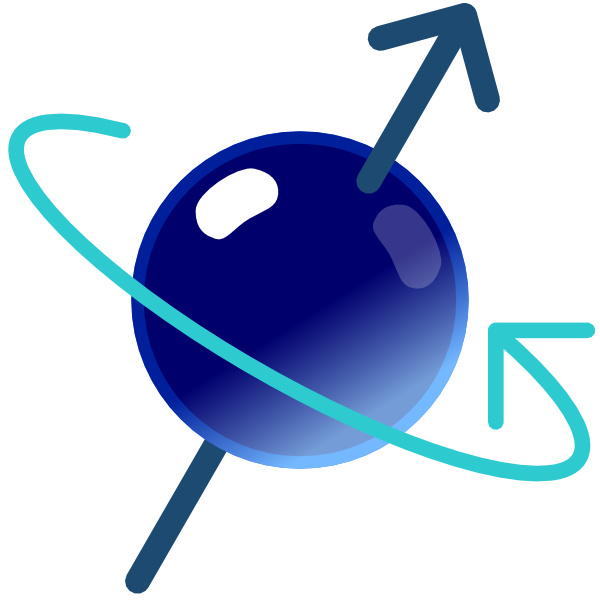
\includegraphics[width=3cm, bb=0 0 1701 1701]{graphics/misc/spin_600x600}
\end{figure*}

Spin containers are nested within a residue container (again graphically depicted in the spin viewer window in figure~\ref{fig: screenshot: spin viewer} on page~\pageref{fig: screenshot: spin viewer}).
Multiple spin containers can exist per residue.
This allows, for example, a single model-free analysis simultaneously on the backbone nitrogen spins, side-chain tryptophan indole nitrogen spins and alpha carbon spins.
Or, for example, studying the pseudocontact shifts for all nitrogen, carbon and proton spins in the molecule simultaneously.

Spin containers can be manually added via the \uf{spin\ufsep{}create} user function in the GUI or prompt/scripting mode:

\begin{lstlisting}
spin.create(spin_num='200', spin_name='NE1')
\end{lstlisting}

The spin viewer window can also be used by right clicking on residue containers.



% Spin ID strings.
\subsubsection{Spin ID strings} \label{sect: spin ID}

Spins are often identified in relax using their ID strings.
The spin ID strings follow the basic construct found in a number of other NMR software such as MOLMOL.
The identification string is composed of three components:

\begin{itemize}
\item The molecule ID token beginning with the \promptstring{\#} character,
\item The residue ID token beginning with the \promptstring{:} character,
\item The atom or spin system ID token beginning with the \promptstring{@} character.
\end{itemize}

Each token can be composed of multiple elements -- one per spin -- separated by the \promptstring{,} character and each individual element can either be a number (which must be an integer, in string format), a name, or a range of numbers separated by the \promptstring{-} character.
Negative numbers are supported.
The full ID string specification is \promptstring{\#<mol\_name> :<res\_id>[, <res\_id>[, <res\_id>, ...]] @<atom\_id>[, <atom\_id>[, <atom\_id>, ...]]}, where the token elements are \promptstring{<mol\_name>}, the name of the molecule, \promptstring{<res\_id>}, the residue identifier which can be a number, name, or range of numbers, \promptstring{<atom\_id>}, the atom or spin system identifier which can be a number, name, or range of numbers.

If one of the tokens is left out then all elements will be assumed to match.
For example if the string does not contain the \promptstring{\#} character then all molecules will match the string.
If only the molecule ID component is specified, then all spins of the molecule will match.

Regular expression can, in some instances, be used to select spins.
For example the string \promptstring{@H*} will select the protons `H', `H2' and `H98'.



% Interatomic data containers.
%%%%%%%%%%%%%%%%%%%%%%%%%%%%%%

\section{Interatomic data containers} \label{sect: interatomic container}

\begin{figure*}[h]
  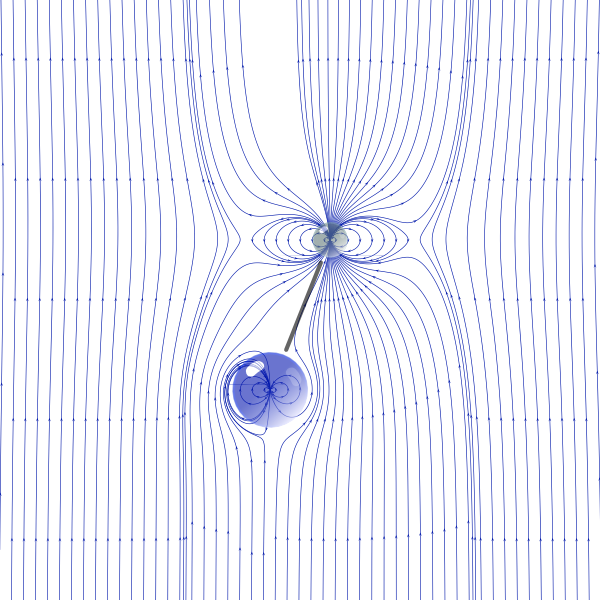
\includegraphics[width=3cm, bb=0 0 1701 1701]{graphics/wizards/dipole_pair/NH_dipole_pair_600x600}
\end{figure*}

Separate from the spin containers, yet strongly linked to them, are the interatomic data containers.
These containers are grouped together within the same data pipe as the spins they point to.
These define interactions between two spins located anywhere within the molecule, residue and spin nested data structure.
These are automatically created when reading in data defined between two spins such as RDCs and NOE distance constraints.
They can also be created using the \uf{interatom\ufsep{}define} user function:

\begin{lstlisting}
interatom.define(spin_id1=':2@N', spin_id2=':2@H')
\end{lstlisting}

As the interatomic data container concept is relatively new, how they are created and handled is likely to evolve and change in the future.



% Setup in the prompt/script UI.
%%%%%%%%%%%%%%%%%%%%%%%%%%%%%%%%

\section{Setup in the prompt/script UI}

Below are three different examples showing how to set up the relax data model for any analysis type requiring spin specific data.


% Spins from structural data.
%~~~~~~~~~~~~~~~~~~~~~~~~~~~~

\subsection{Script mode -- spins from structural data} \label{sect: script - structural data}

\begin{figure*}[h]
  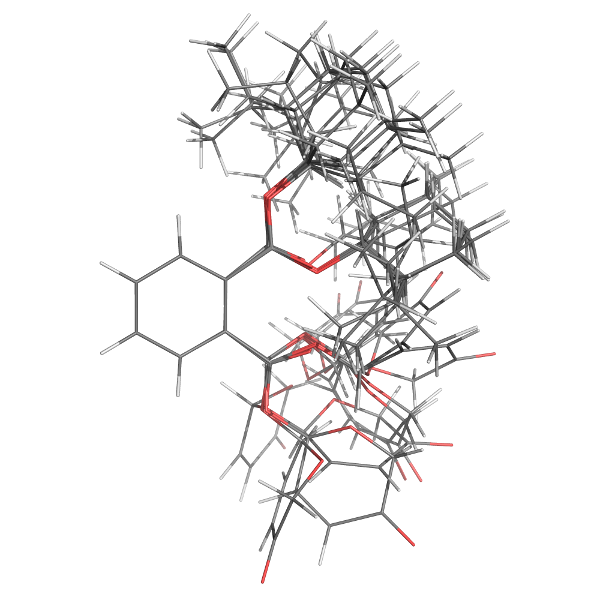
\includegraphics[width=3cm, bb=0 0 1701 1701]{graphics/misc/n_state_model/phthalic_acid_ens_600x600}
\end{figure*}

3D structural data is stored at the level of the current data pipe.
This data is completely separate from the molecule, residue and spin data structure.
However the structural data can be used to generate the spin containers.
For example for the nitrogen relaxation in a model-free analysis where both the nitrogen and proton are needed to define the magnetic dipole-dipole relaxation:

\begin{lstlisting}
# Create a data pipe.
pipe.create(pipe_name='ellipsoid', pipe_type='mf')

# Load the PDB file.
structure.read_pdb('1f3y.pdb')

# Set up the 15N and 1H backbone spins.
structure.load_spins('@N', ave_pos=True)
structure.load_spins('@H', ave_pos=True)

# Set up the 15N and 1H for the tryptophan indole ring.
structure.load_spins('@NE1', ave_pos=True)
structure.load_spins('@HE1', ave_pos=True)

# Define the spin isotopes.
spin.isotope('15N', spin_id='@N*')
spin.isotope('1H', spin_id='@H*')
\end{lstlisting}

The \uf{structure\ufsep{}read\ufus{}pdb} user function will load the structural data into the current data pipe, and the \uf{structure\ufsep{}load\ufus{}spins} user function will create the molecule, residue, and spin containers as needed.
This will also load atomic position information into the matching spin containers.
The \uf{spin\ufsep{}isotope} user function is required to define the magnetic dipole-dipole interaction and is information not present in the PDB file.

Note that if structural data from the PDB is used to generate the spin containers, then all subsequent data loaded into relax must follow the exact naming convention from the PDB file.
Automatic residue name matching (i.e. `GLY' = `Gly' = `gly' = `G') is currently not supported.



% Spins from a sequence file.
%~~~~~~~~~~~~~~~~~~~~~~~~~~~~

\subsection{Script mode -- spins from a sequence file} \label{sect: script - sequence file}

\begin{figure*}[h]
  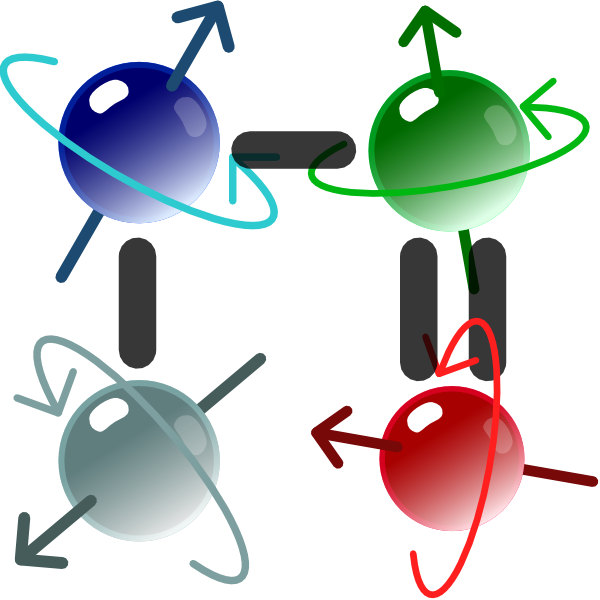
\includegraphics[width=3cm, bb=0 0 1701 1701]{graphics/misc/sequence_600x600}
\end{figure*}

Alternatively to setting up the molecule, residue, and spin containers via 3D structural data, a plain text columnar formatted file can be used.
This is useful for when no 3D structure exists for the molecule.
It also has the advantage that the residue and atom names need not conform to the PDB standard.
An example for reading sequence data is:

\begin{lstlisting}
# Create a data pipe.
pipe.create(pipe_name='R1 1200', pipe_type='relax_fit')

# Set up the 15N spins.
sequence.read(file='noe.500.out', mol_name_col=1, res_num_col=2, res_name_col=3, spin_num_col=4, spin_name_col=5)
spin.element(element='N', spin_id='@N*')
spin.isotope('15N', spin_id='@N')
\end{lstlisting}

Here the molecule, residue, and spin information is extracted from the \promptstring{noe.500.out} file which could look like:

{\scriptsize \begin{verbatim}
# mol_name          res_num  res_name  spin_num  spin_name  value             error               
Ap4Aase_new_3_mol1  1        GLY       1         N          None              None                
Ap4Aase_new_3_mol1  2        PRO       11        N          None              None                
Ap4Aase_new_3_mol1  3        LEU       28        N          None              None                
Ap4Aase_new_3_mol1  4        GLY       51        N          0.03892194698453  0.01903177024613    
Ap4Aase_new_3_mol1  5        SER       59        N          0.31240422567912  0.01859693729836    
Ap4Aase_new_3_mol1  6        MET       71        N          0.42850831873249  0.0252585632304     
Ap4Aase_new_3_mol1  7        ASP       91        N          0.53054928103134  0.02799062314416    
Ap4Aase_new_3_mol1  8        SER       104       N          0.56528429775819  0.02170612146773    
Ap4Aase_new_3_mol1  9        PRO       116       N          None              None                
Ap4Aase_new_3_mol1  40       TRP       685       N          0.65394813490548  0.03830061886537    
Ap4Aase_new_3_mol1  40       TRP       698       NE1        0.67073879732046  0.01426066343831    
\end{verbatim}} \label{verb: noe.500.out}

The file can contain columns for the molecule name, the residue name and number, and the spin name and number in any order though not all are needed.
For example for a single protein system, the molecule name, residue name and spin number are nonessential.
Or for an organic molecule, the molecule name, residue name and number and spin number could be nonessential.
The subsequent user functions in the above example are used to set up the spin containers appropriately for a model-free analysis.
These are not required in the automatic analysis of GUI as these user functions will be presented to you when adding relaxation data, or when clicking on the heteronucleus and proton buttons (\guibutton{X isotope} and \guibutton{H isotope}).

In the GUI, the creation of molecule, residue, and spin containers from a sequence file is also available via the \gui{Load spins} wizard within the spin viewer window (\textit{vide supra}).


% Manual construction.
%~~~~~~~~~~~~~~~~~~~~~

\subsection{Script mode -- manual construction} \label{sect: script - manual construction}

For the masochists out there, the full molecule, residue and spin data structure can be manually constructed.
For example:

\begin{lstlisting}
# Manually create the molecule, residue, and spin containers.
molecule.create(mol_name='Ap4Aase', mol_type='protein')
residue.create(res_num=1,  res_name='GLY')
residue.create(res_num=3,  res_name='LEU')
residue.create(res_num=96, res_name='TRP')
spin.create(res_num=1,  spin_name='N')
spin.create(res_num=3,  spin_name='N')
spin.create(res_num=96, spin_name='N')
spin.create(res_num=96, spin_name='NE1')
\end{lstlisting}

These user functions can be repeated until the full sequence has been constructed.



% Setup in the GUI.
%%%%%%%%%%%%%%%%%%%

\section{Setup in the GUI}


% The data pipe.
%~~~~~~~~~~~~~~~

\subsection{GUI mode -- setting up the data pipe} \label{sect: GUI - data pipe}

In the GUI, the most common way to create the data pipe is to initialise one of the auto-analyses via the analysis selection wizard (see Figure~\ref{fig: screenshot: analysis wizard} on page~\pageref{fig: screenshot: analysis wizard}).
The initialisation will create the appropriate starting data pipe.
Alternatively the data pipe editor can be used (see Figure~\ref{fig: screenshot: pipe editor} on page~\pageref{fig: screenshot: pipe editor}).
Or the \guimenuitemthree{User functions}{pipe}{create} menu item can be selected for graphical access to the \uf{pipe\ufsep{}create} user function.



% Spins from structural data.
%~~~~~~~~~~~~~~~~~~~~~~~~~~~~

\subsection{GUI mode -- spins from structural data} \label{sect: GUI - structural data}

For this section, the example of protein $^{15}$N relaxation data will be used to illustrate how to set up the data structures.
To manipulate the molecule, residue and spin data structures in the GUI, the most convenient option is to use the spin viewer window (see Figure~\ref{fig: screenshot: spin viewer} on page~\pageref{fig: screenshot: spin viewer}).
This window can be opened in four ways:

\begin{itemize}
\item The \guimenuitemtwo{View}{Spin viewer} menu item,
\item The \shortcutkey{Ctrl+T} key combination,
\item The spin viewer icon in the toolbar (represented by the blue spin icon),
\item The \guibutton{Spin editor} button part of the \gui{Spin systems} GUI element in the specific analysis tabs.
\end{itemize}

You will then see:

\begin{minipage}[h]{\linewidth}
  \centerline{
    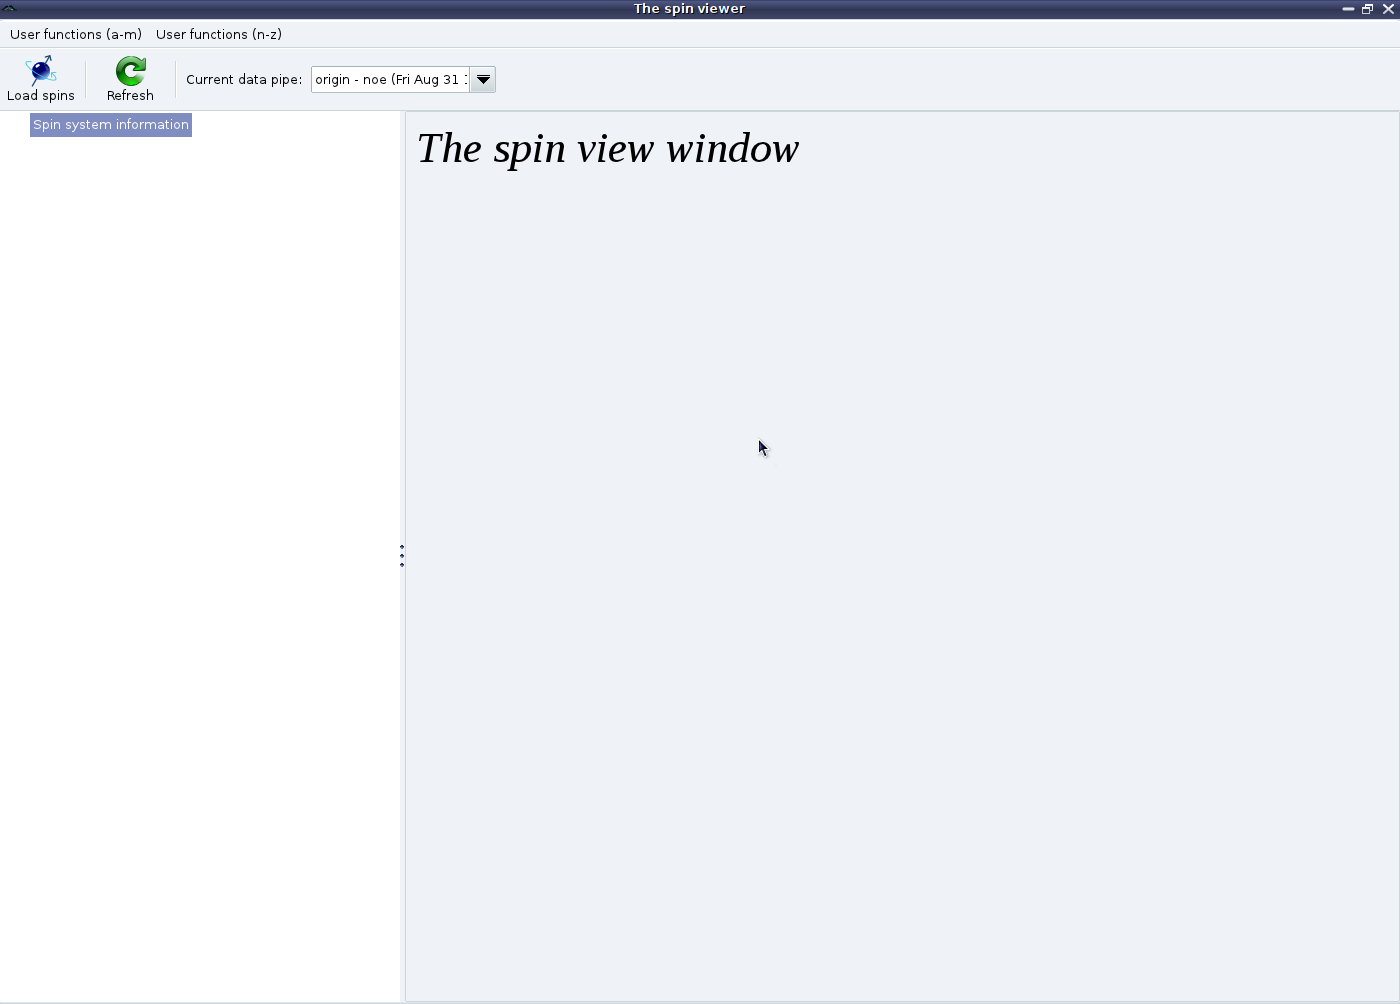
\includegraphics[
      width=0.8\textwidth,
      bb=14 14 1415 1019
    ]
    {graphics/screenshots/spin_viewer/blank}
  }
  \label{figure: spin viewer blank}
\end{minipage}

At this point, click on the \guibutton{Load spins} button (or the \guimenuitemone{Load spins} menu entry from the right click pop up menu) to launch the spin loading wizard.
A number of options will be presented to you: 

\begin{minipage}[h]{\linewidth}
  \centerline{
    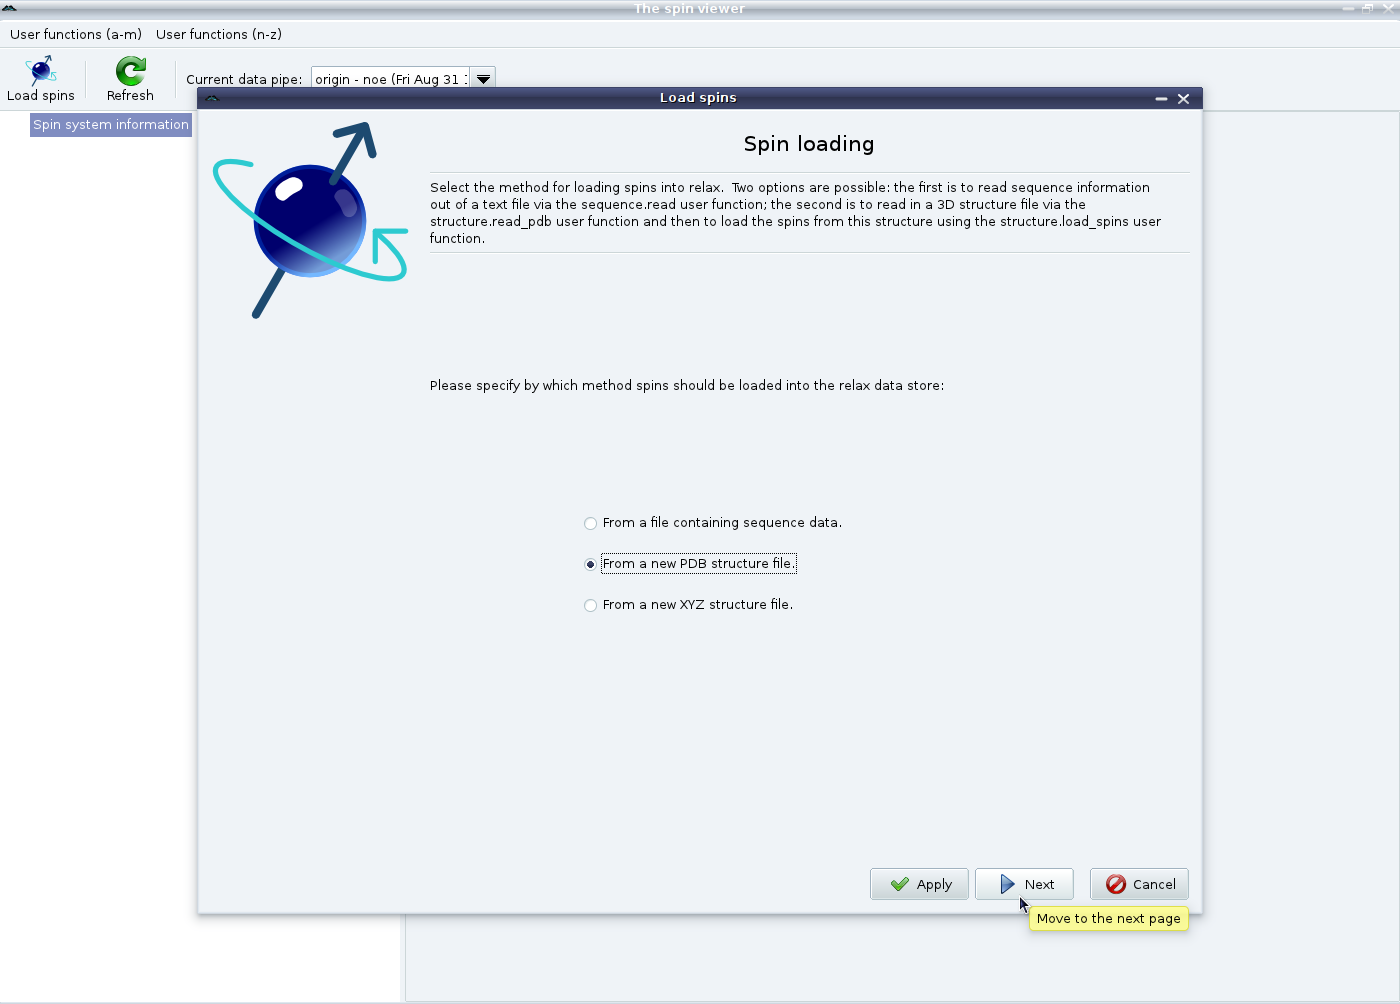
\includegraphics[
      width=0.8\textwidth,
      bb=14 14 1415 1019
    ]
    {graphics/screenshots/spin_viewer/wizard_start}
  }
  \label{figure: spin viewer wizard start}
\end{minipage}

Here the spins will be loaded from a PDB file.
If you do not have a 3D structure file, please see the next section.
After selecting \gui{From a new PDB structure file} and clicking on \guibutton{Next}, you will see:

\begin{minipage}[h]{\linewidth}
  \centerline{
    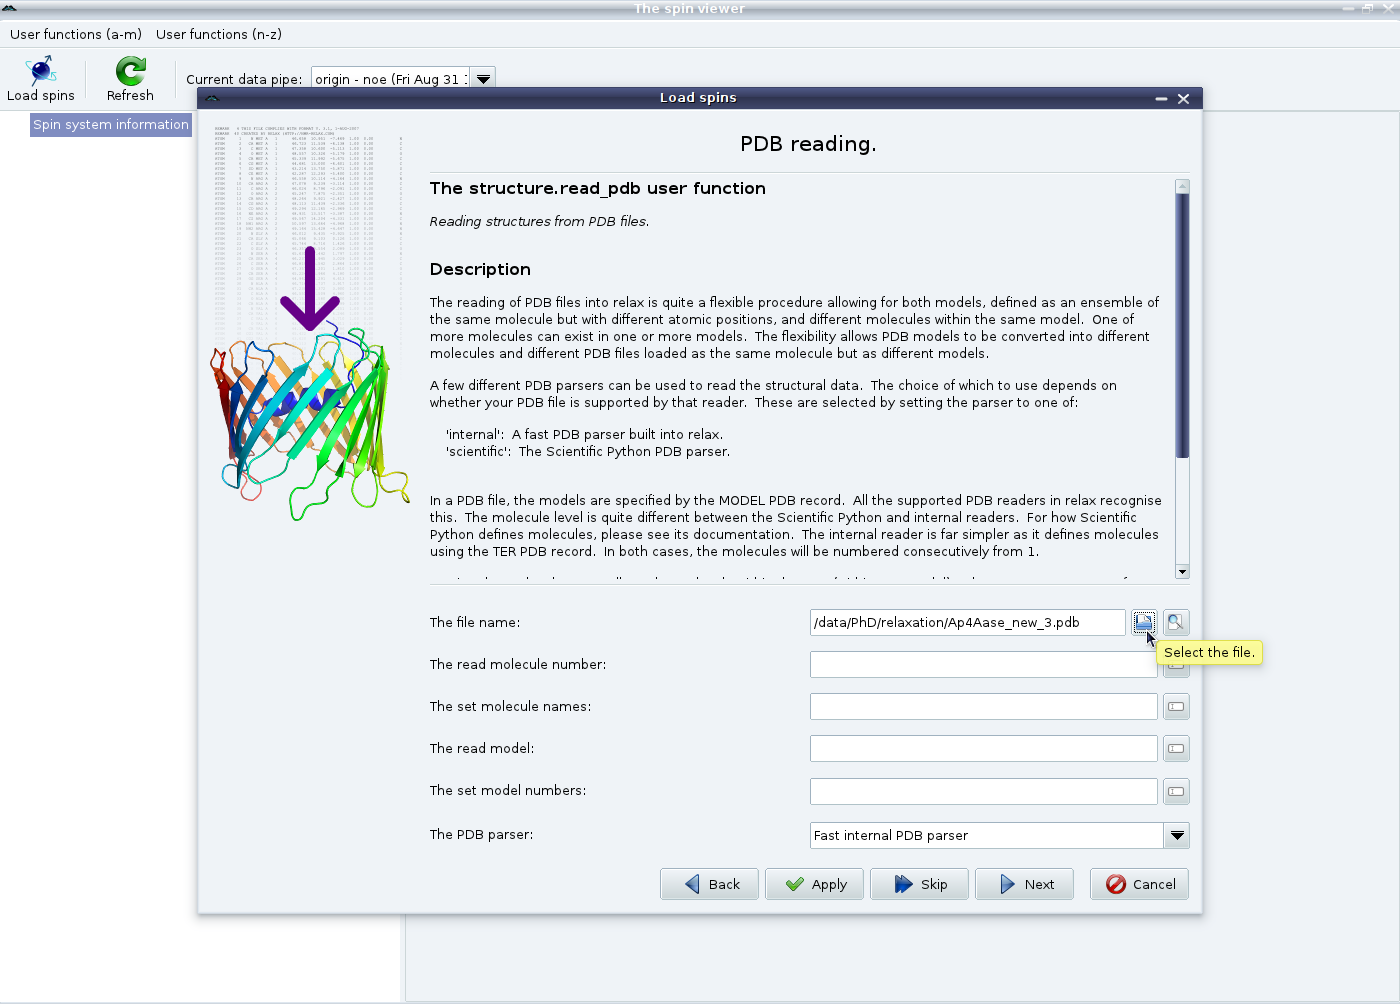
\includegraphics[
      width=0.8\textwidth,
      bb=14 14 1415 1019
    ]
    {graphics/screenshots/spin_viewer/wizard_read_pdb}
  }
\end{minipage}

Now select the PDB file you wish to use.
The other options in this screen allow you to handle NMR models and multiple molecules within a single PDB file.
These options are explained in the window.
Hovering the mouse over the options will give additional hints.
In this example, the \nth{3} model from the 1F3Y PDB file will be read and the single molecule will be named \guistring{Ap4Aase} to override the default naming of \guistring{1f3y\_mol1}.
Now click on \guibutton{Next} to bring up the spin loading page:

\begin{minipage}[h]{\linewidth}
  \centerline{
    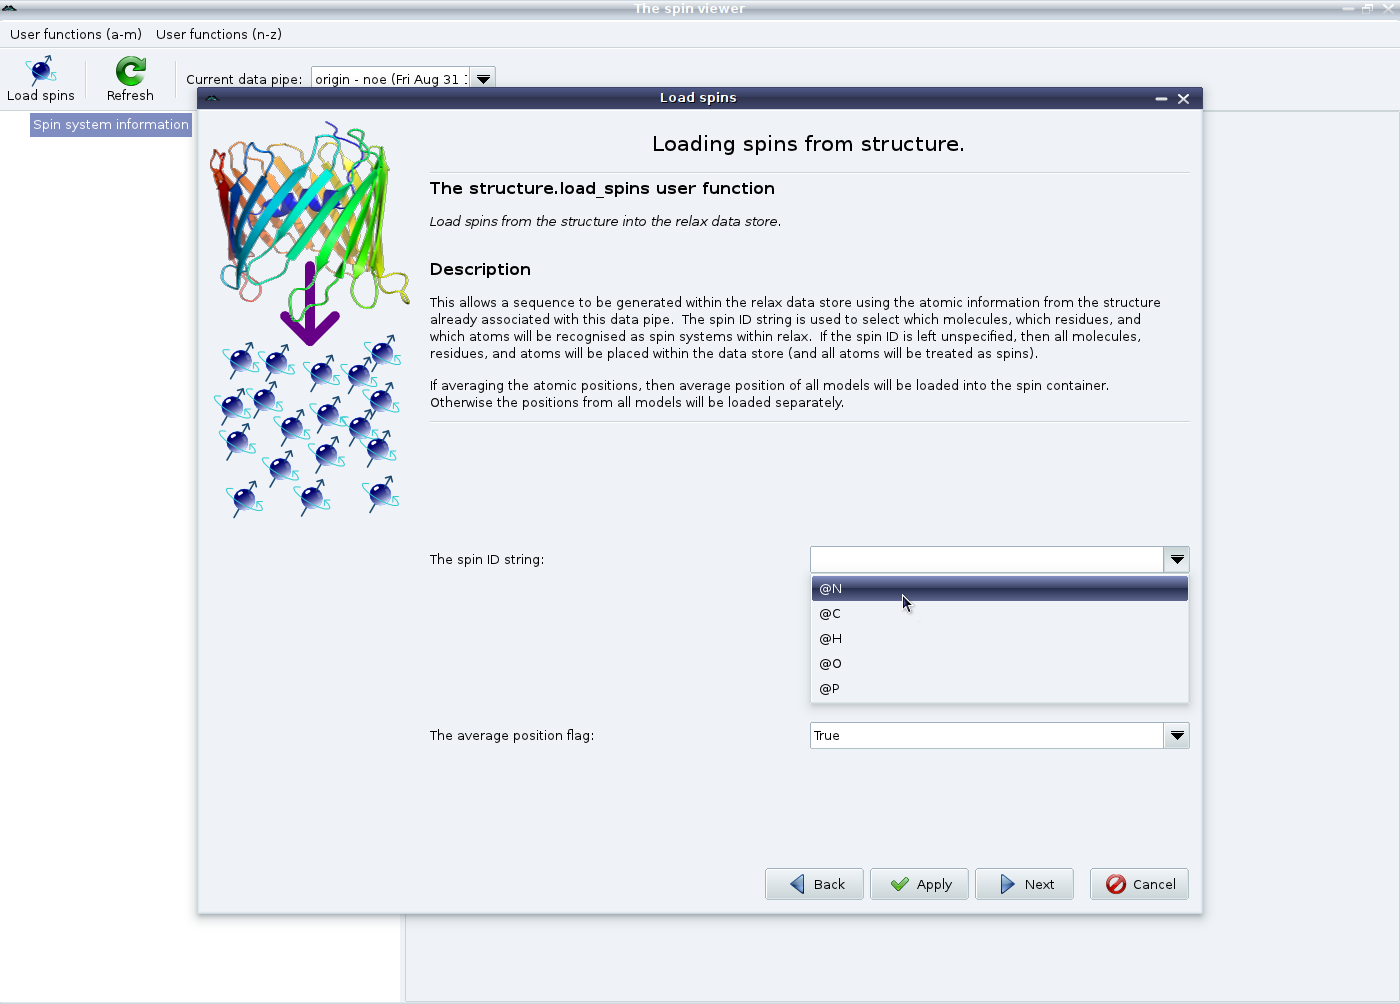
\includegraphics[
      width=0.8\textwidth,
      bb=14 14 1415 1019
    ]
    {graphics/screenshots/spin_viewer/wizard_load_spins_n}
  }
\end{minipage}

This is a bit more complicated.
In this example we are studying the backbone dynamics of $^{15}$N spins of a protein.
Therefore first set the spin ID string to \guistring{@N} (which can be selected from the pull down) and click on \guibutton{Apply} to set up the backbone spins.
Do not click on \guibutton{Next} yet.
If the current study requires the specification of the dipole-dipole interaction (for example if it involves relaxation data -- model-free analyses, consistency testing, reduced spectral density mapping; or the dipolar coupling -- the N-state model or ensemble analyses, the Frame Order theory) you will also need to load the $^1$H spins as well.
Therefore set the spin ID string to \guistring{@H} and click on \guibutton{Apply} again.


\begin{minipage}[h]{\linewidth}
  \centerline{
    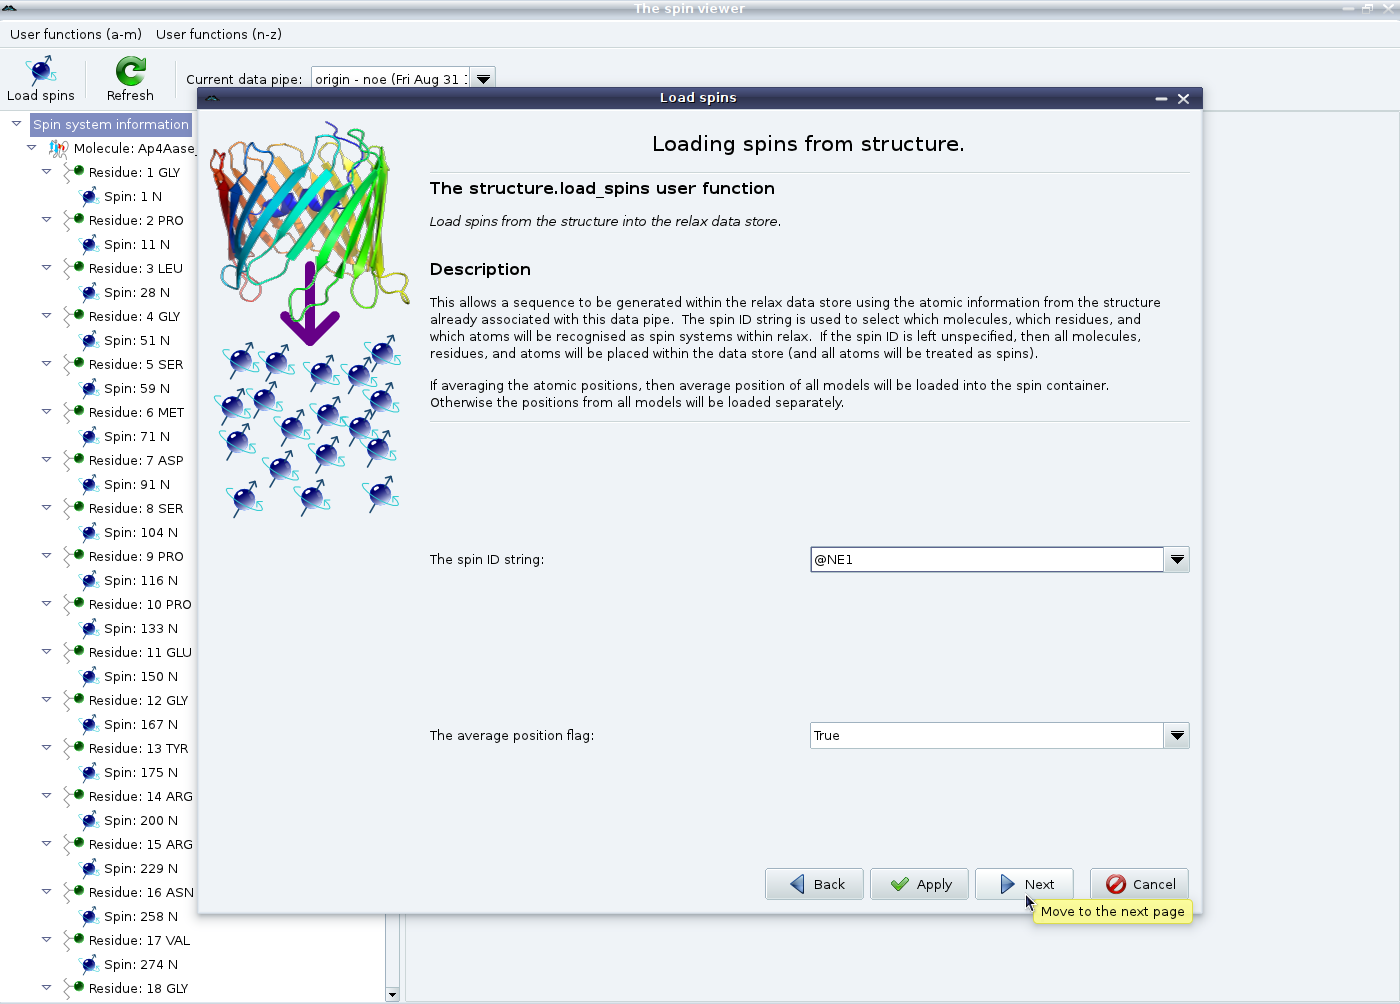
\includegraphics[
      width=0.8\textwidth,
      bb=14 14 1415 1019
    ]
    {graphics/screenshots/spin_viewer/wizard_load_spins_ne1}
  }
\end{minipage}

Now change the spin ID string to \guistring{@NE1} and then click on \guibutton{Next} (or \guibutton{Apply} if the Trp protons \guistring{@HE1} need to be loaded as well).
This will add spin containers for the tryptophan indole $^{15}$N spins.
Finally click on \guibutton{Finish} to exit the wizard:

\begin{minipage}[h]{\linewidth}
  \centerline{
    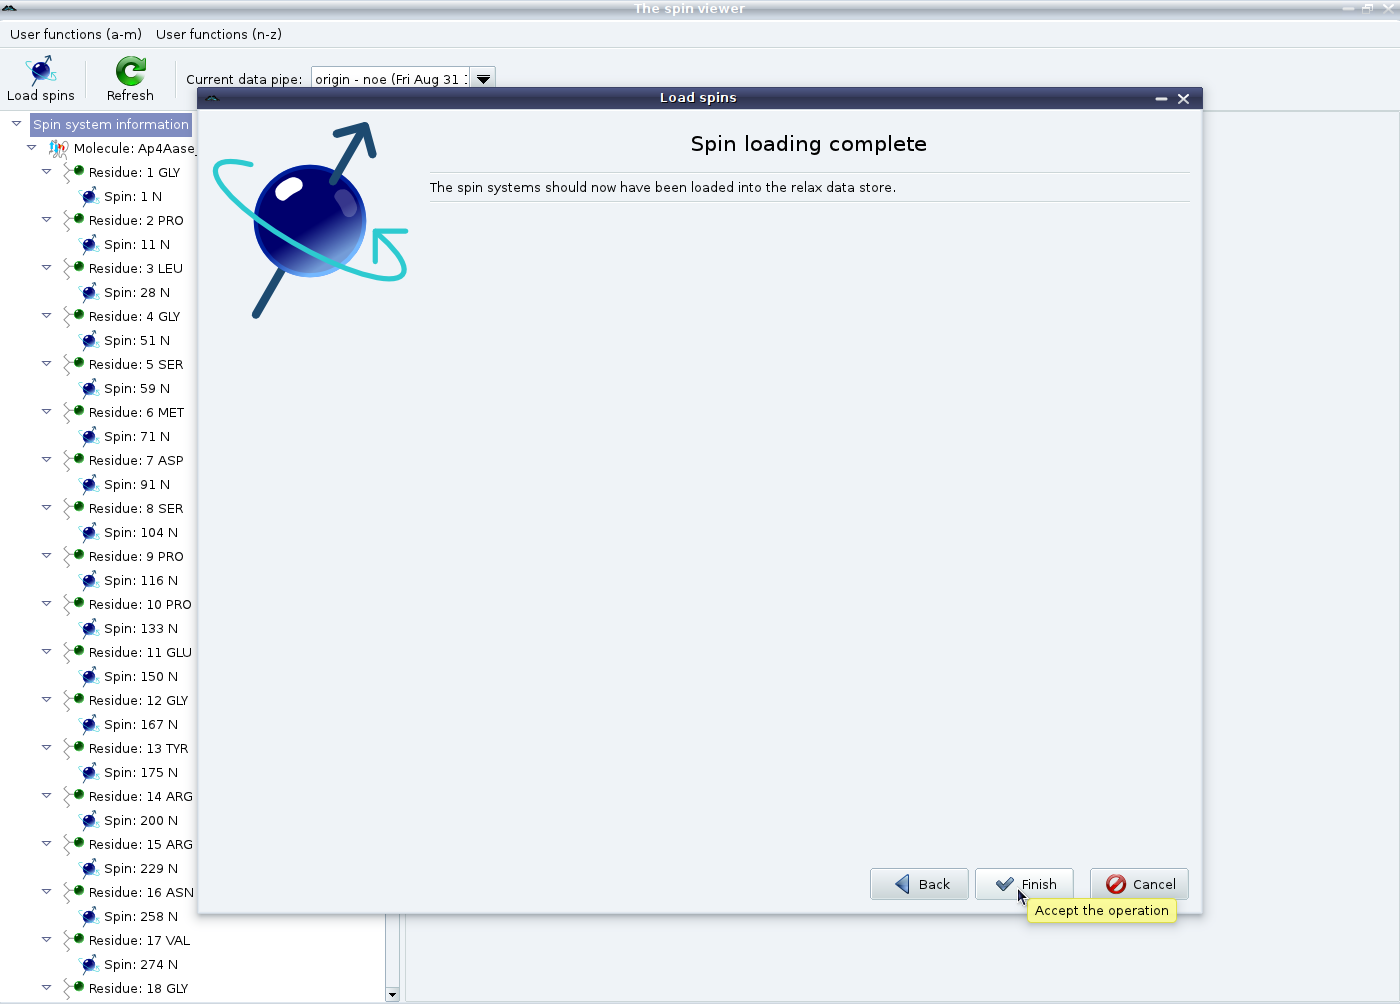
\includegraphics[
      width=0.8\textwidth,
      bb=14 14 1415 1019
    ]
    {graphics/screenshots/spin_viewer/wizard_end}
  }
\label{figure: spin viewer end}
\end{minipage}

You should now see something such as:

\begin{minipage}[h]{\linewidth}
  \centerline{
    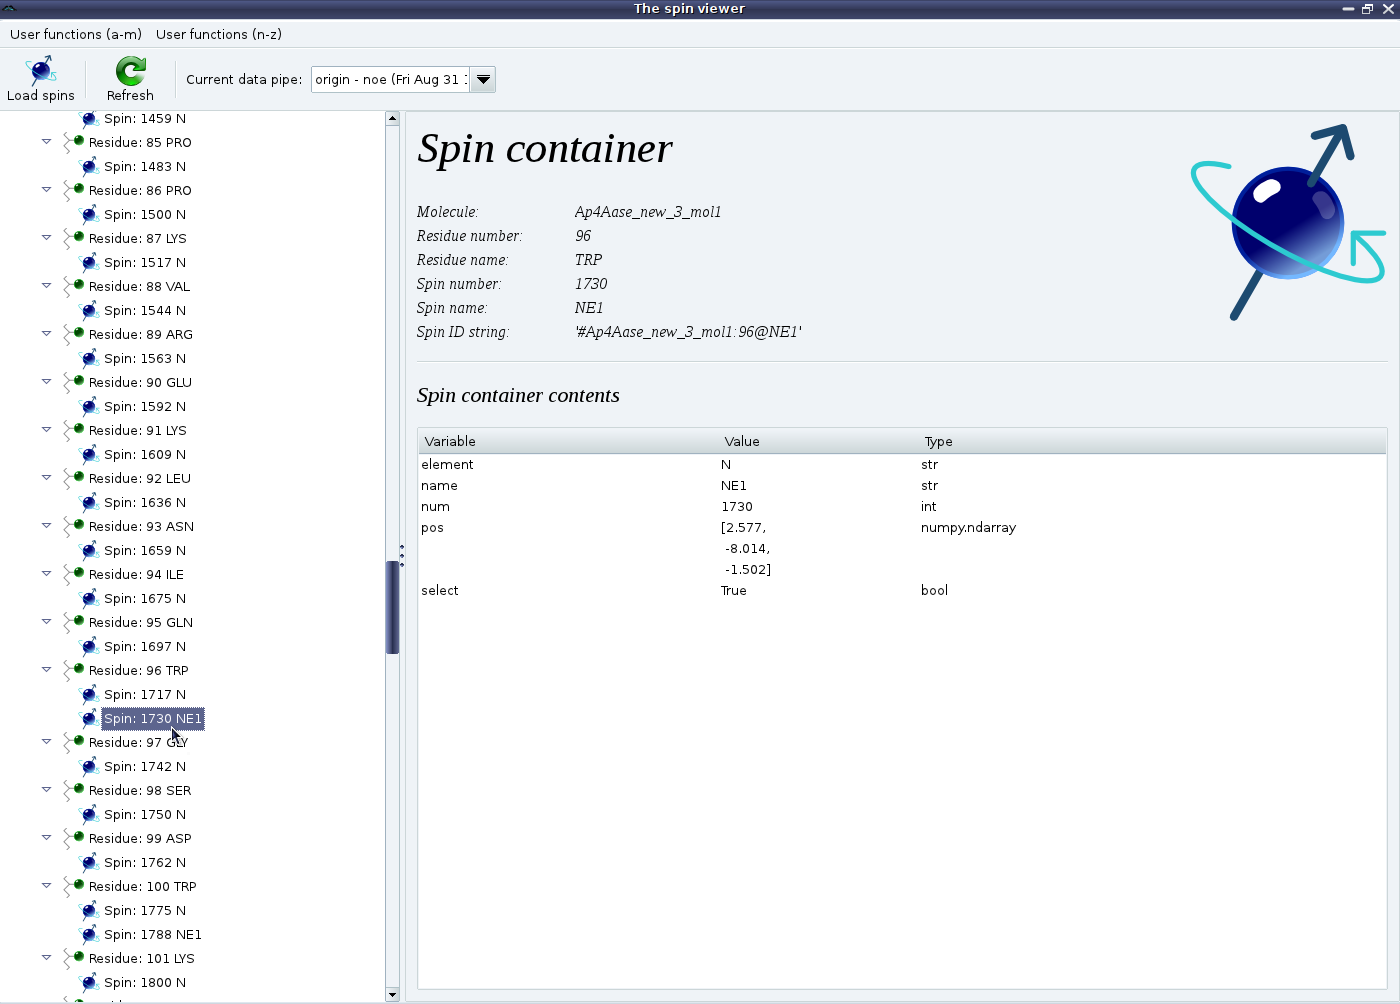
\includegraphics[
      width=0.8\textwidth,
      bb=14 14 1415 1019
    ]
    {graphics/screenshots/spin_viewer/full}
  }
\end{minipage}

If the $^1$H spins have been loaded as well, then you should see exactly twice as many spin containers as shown above.


% Spins from a sequence file.
%~~~~~~~~~~~~~~~~~~~~~~~~~~~~

\subsection{GUI mode -- spins from a sequence file} \label{sect: GUI - sequence file}

Starting from the empty spin viewer window on page~\pageref{figure: spin viewer blank}), click on the \guibutton{Load spins} button.
You will then see the spin loading wizard (see page~\pageref{figure: spin viewer wizard start}).
Select the option for reading data from a sequence file.
You should then see:

\begin{minipage}[h]{\linewidth}
  \centerline{
    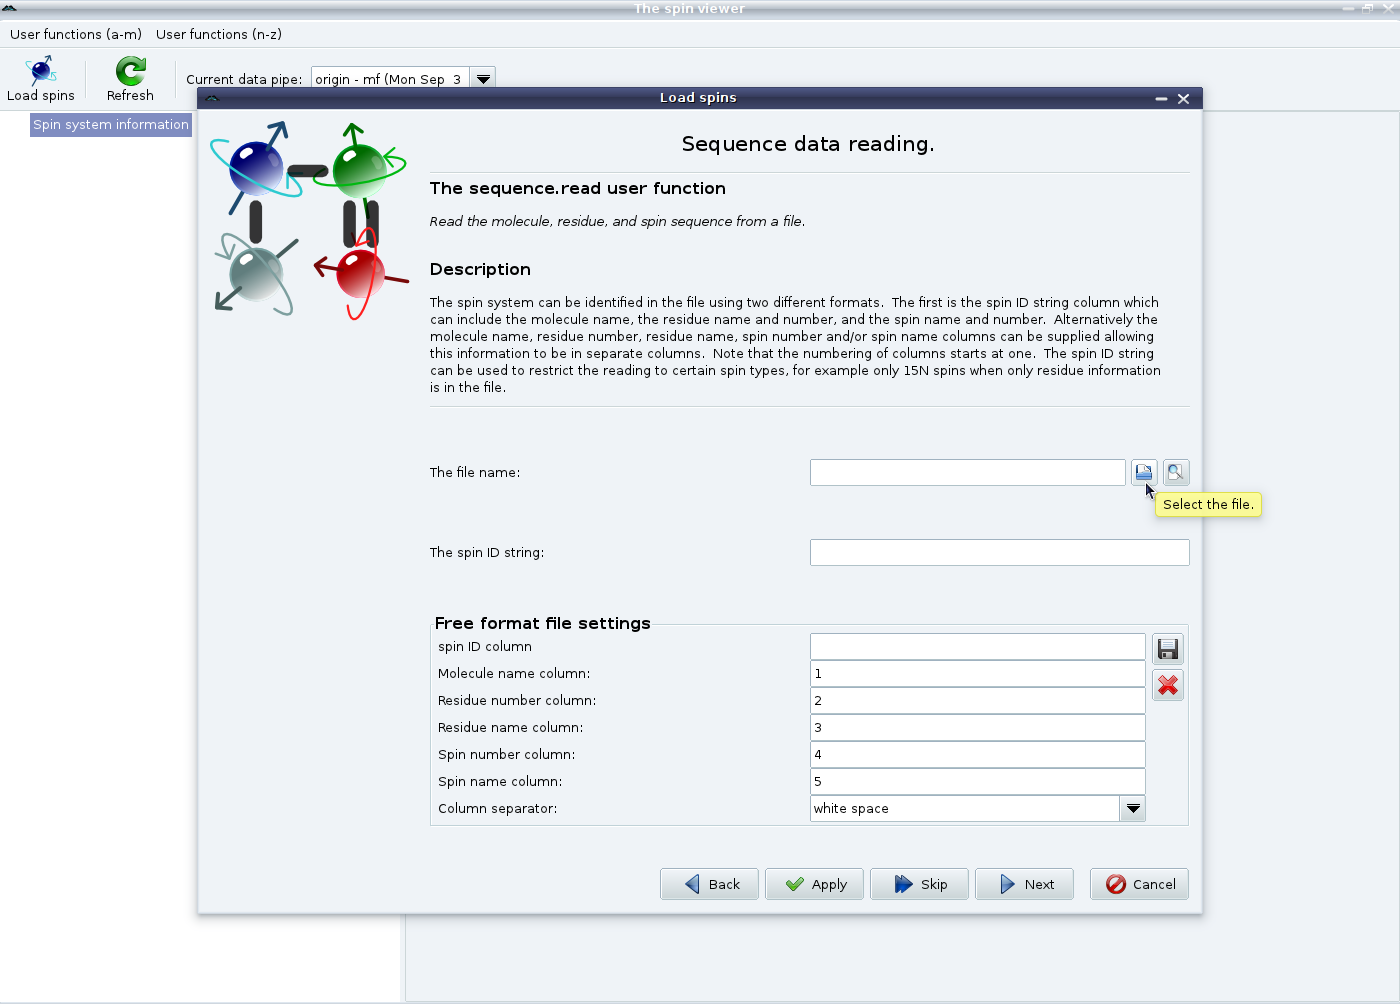
\includegraphics[
      width=0.8\textwidth,
      bb=14 14 1415 1019
    ]
    {graphics/screenshots/spin_viewer/wizard_sequence}
  }
\end{minipage}

Select the file to load and change the \gui{Free format file settings} as needed.
An example of a suitable format is given on page~\pageref{verb: noe.500.out}.
Click on \guibutton{Next} to reach the wizard ending page (see~\pageref{figure: spin viewer end}).
Finally click on \guibutton{Finish} to exit the wizard.


% Manual construction.
%~~~~~~~~~~~~~~~~~~~~~

\subsection{GUI mode -- manual construction} \label{sect: GUI - manual construction}

Just as in the prompt/script UI mode, the molecules, residues and spins can be manually added.
First add a molecule by right clicking on the \gui{Spin system information} element and selecting the relevant entry in the popup menu.
Then right click on the newly created molecule container to add residues, and right click on residue containers to add spins.


% Deselect spins.
%~~~~~~~~~~~~~~~~

\subsection{GUI mode -- deselect spins} \label{sect: GUI - deselect spins}

To deselect spins (for example if they are unresolved, overlapping peaks), click on the \guimenuitemthree{User functions}{deselect}{read} menu item from the main relax window or the spin viewer window:

\begin{minipage}[h]{\linewidth}
  \centerline{
    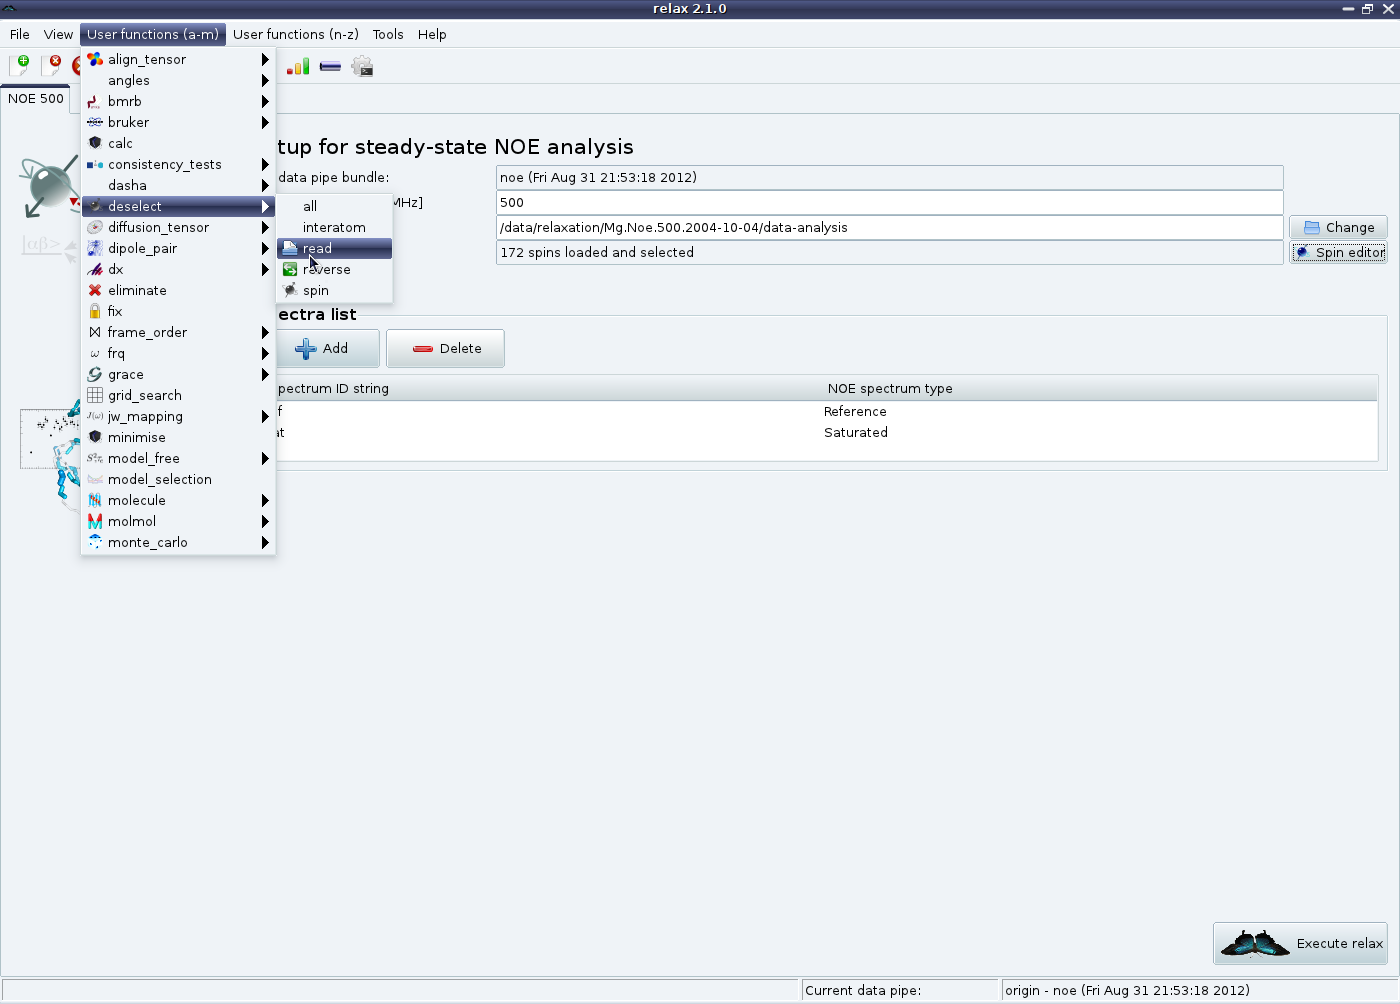
\includegraphics[
      width=0.8\textwidth,
      bb=14 14 1415 1019
    ]
    {graphics/screenshots/noe_analysis/analysis_tab3}
  }
\end{minipage}

Select the file listing the unresolved spins and change the column numbers in the \gui{Free format file settings} GUI element as needed: 

\begin{minipage}[h]{\linewidth}
  \centerline{
    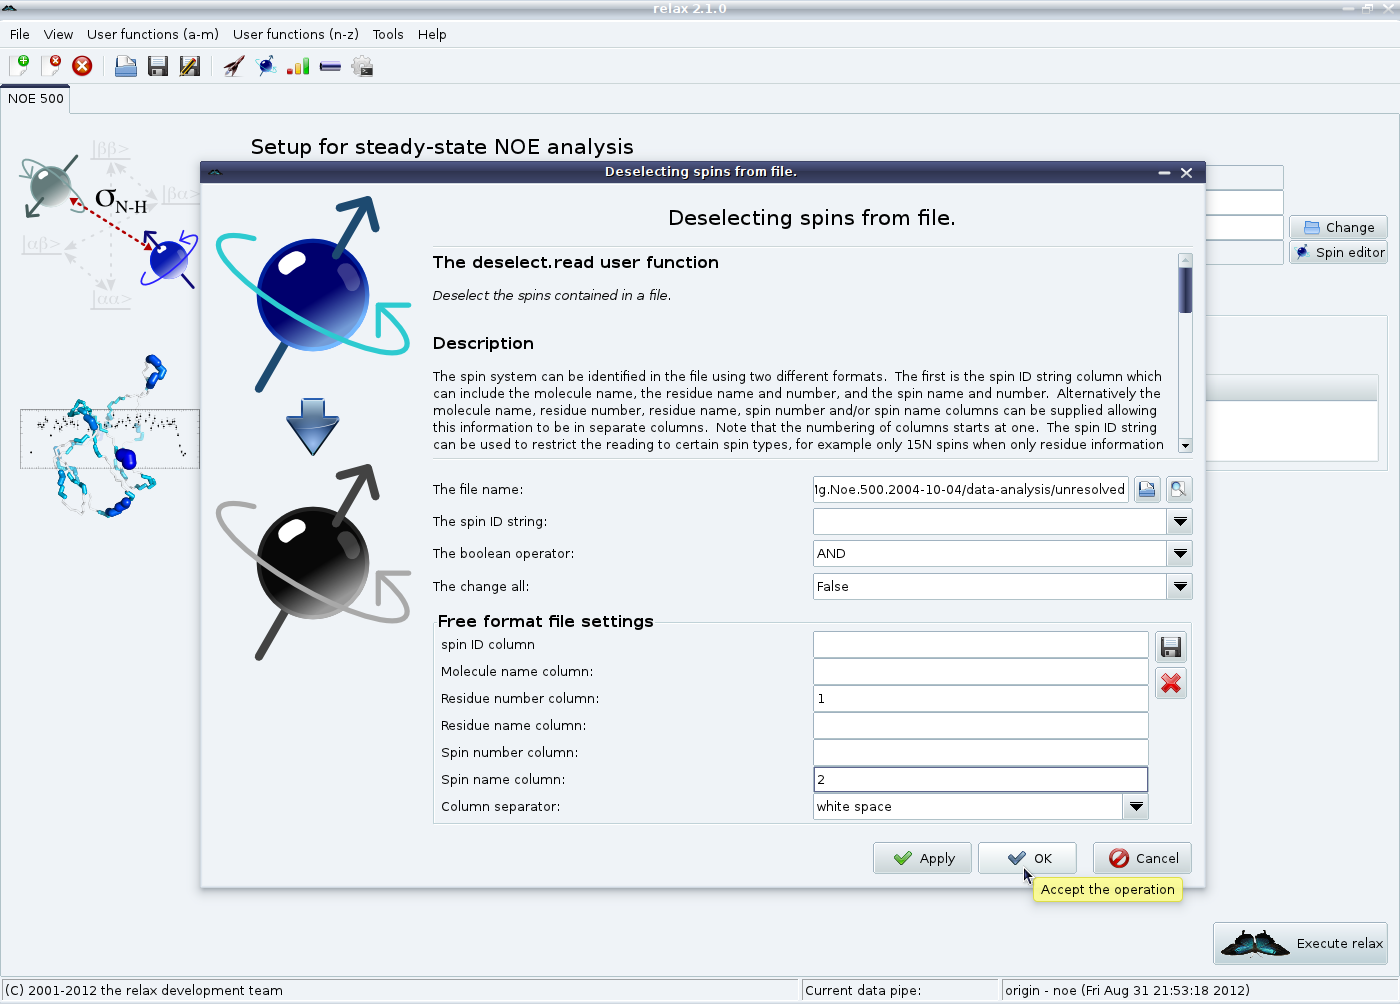
\includegraphics[
      width=0.8\textwidth,
      bb=14 14 1415 1019
    ]
    {graphics/screenshots/noe_analysis/deselect}
  }
\end{minipage}

Alternatively the spin editor window can be reopened and the spins manually deselected by right clicking on them and selecting \gui{Deselect}.
Returning to the spin editor window, you should now see certain spins coloured grey:

\begin{minipage}[h]{\linewidth}
  \centerline{
    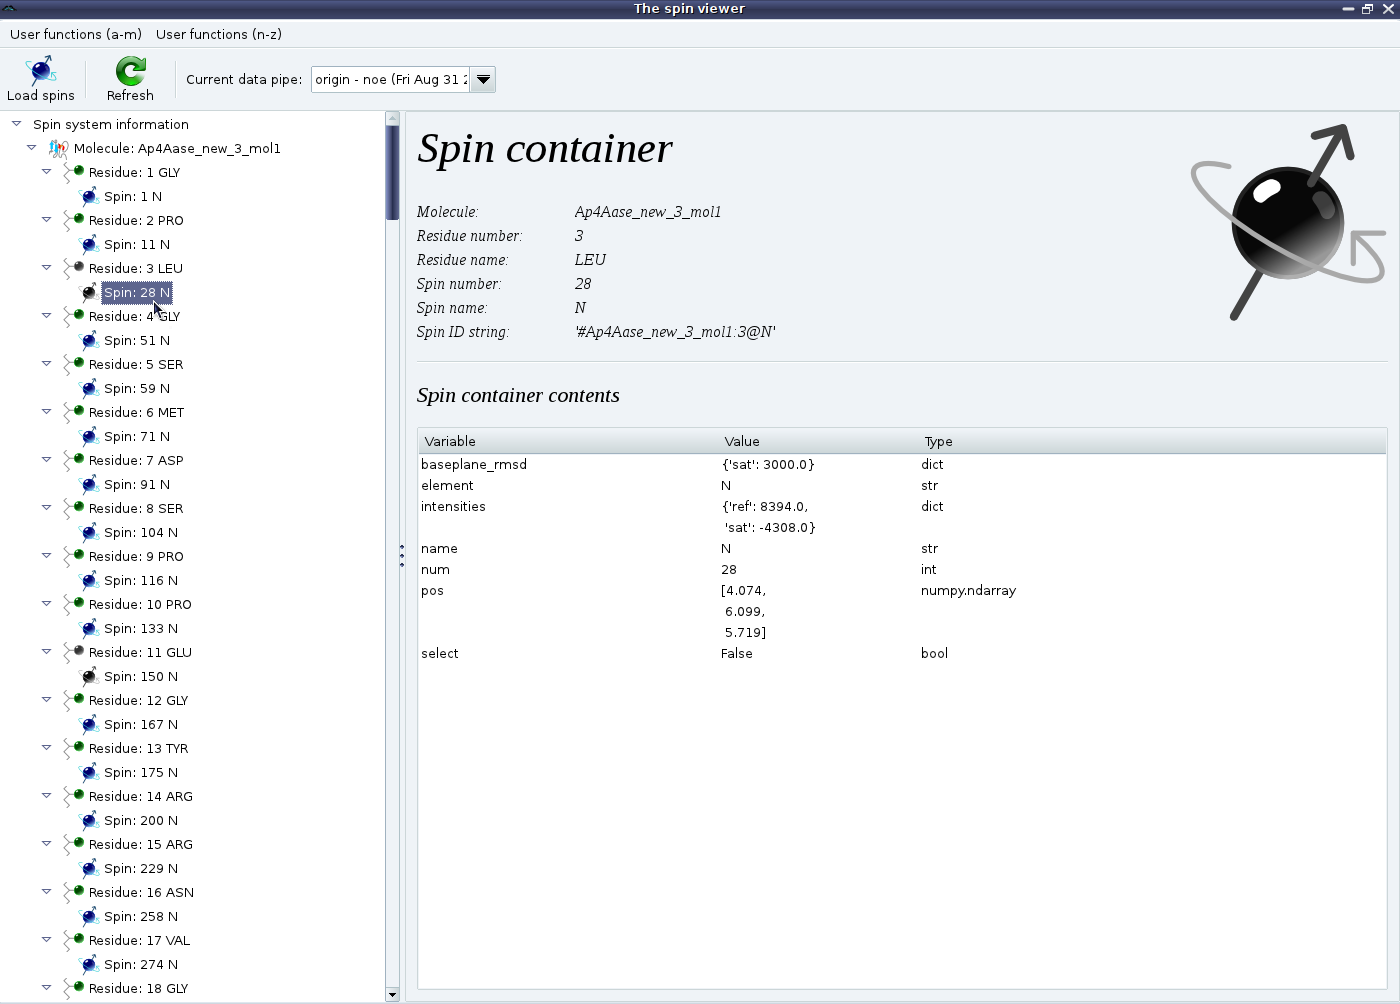
\includegraphics[
      width=0.8\textwidth,
      bb=14 14 1415 1019
    ]
    {graphics/screenshots/spin_viewer/deselect}
  }
\end{minipage}



% The next steps.
%%%%%%%%%%%%%%%%%

\section{The next steps}

This chapter presented the basics of setting up the relax data store, concepts which are needed for all analysis types built into relax.
The next chapters will introduce specific analyses types -- the steady-state NOE, $\Rone$ and $\Rtwo$ relaxation curve-fitting, and the automated full model-free analysis protocol of \citet{dAuvergneGooley07,dAuvergneGooley08b} -- which build on the ideas introduced here.

% Calculating the NOE.
%%%%%%%%%%%%%%%%%%%%%%

\chapter{Calculating the NOE} \label{ch: NOE}
\index{NOE|textbf}


\begin{figure*}[h]
  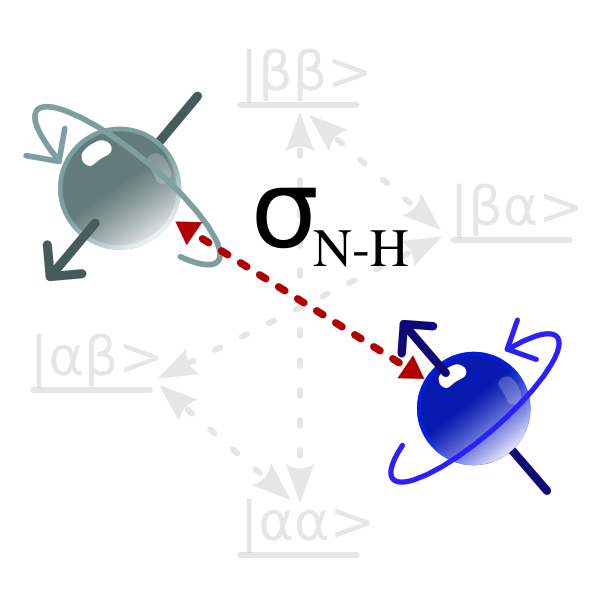
\includegraphics[width=5cm, bb=0 0 1701 1701]{graphics/analyses/noe_600x600}
\end{figure*}


% Introduction.
%%%%%%%%%%%%%%%

\section{Introduction to the steady-state NOE}

The calculation of NOE values is a straight forward and quick procedure which involves two components -- the calculation of the value itself and the calculation of the errors.
To understand the steps involved the execution of a sample NOE calculation script will be followed in detail.
Then the same operations will be presented for the perspective of the graphical user interface.



% From spectra to peak intensities.
%%%%%%%%%%%%%%%%%%%%%%%%%%%%%%%%%%%

\section{From spectra to peak intensities for the NOE}

For a set of recommendations for how to obtain the best quality relaxation rates, please see section~\ref{sect: spectra to intensities} on page~\pageref{sect: spectra to intensities}.
In summary the following are important -- temperature control (though the standard steady-state NOE single FID interleaved pulse sequences are fine), per-experiment temperature calibration, spectral processing with massive zero-filling and no baseplane rolling, and using an averaged peak list for determining the peak heights.



% Script UI.
%%%%%%%%%%%%

\section{Calculation of the NOE in the prompt/script UI mode}


% The sample script.
%~~~~~~~~~~~~~~~~~~~

\subsection{NOE script mode -- the sample script}

This sample script can be found in the \directory{sample\osus{}scripts} directory and will be used as the template for the next sections describing how to use relax.

\begin{lstlisting}
# Script for calculating NOEs.

# Create the data pipe.
pipe.create('NOE', 'noe')

# Load the sequence from a PDB file.
structure.read_pdb('Ap4Aase_new_3.pdb')
structure.load_spins(spin_id='@N')
structure.load_spins(spin_id='@NE1')

# Load the reference spectrum and saturated spectrum peak intensities.
spectrum.read_intensities(file='ref.list', spectrum_id='ref_ave')
spectrum.read_intensities(file='sat.list', spectrum_id='sat_ave')

# Set the spectrum types.
noe.spectrum_type('ref', 'ref_ave')
noe.spectrum_type('sat', 'sat_ave')

# Set the errors.
spectrum.baseplane_rmsd(error=3600, spectrum_id='ref_ave')
spectrum.baseplane_rmsd(error=3000, spectrum_id='sat_ave')

# Individual residue errors.
spectrum.baseplane_rmsd(error=122000, spectrum_type='ref', res_num=114)
spectrum.baseplane_rmsd(error=8500, spectrum_type='sat', res_num=114)

# Peak intensity error analysis.
spectrum.error_analysis()

# Deselect unresolved spins.
deselect.read(file='unresolved', res_num_col=1, spin_name_col=2)

# Calculate the NOEs.
calc()

# Save the NOEs.
value.write(param='noe', file='noe.out', force=True)

# Create Grace files.
grace.write(y_data_type='peak_intensity', file='intensities.agr', force=True)
grace.write(y_data_type='noe', file='noe.agr', force=True)

# View the Grace files.
grace.view(file='intensities.agr')
grace.view(file='noe.agr')

# Write the results.
results.write(file='results', dir=None, force=True)

# Save the program state.
state.save('save', force=True)
\end{lstlisting}



% Initialisation of the data pipe.
%~~~~~~~~~~~~~~~~~~~~~~~~~~~~~~~~~

\subsection{NOE script mode -- initialisation of the data pipe} \label{NOE initialisation}

The start of this sample script is very similar to that of the relaxation curve-fitting calculation on page~\pageref{Rx initialisation}.
The command

\begin{lstlisting}[firstnumber=3]
# Create the data pipe.
pipe.create('NOE', 'noe')
\end{lstlisting}

initialises the data pipe labelled \promptstring{NOE}.
The data pipe type is set to the NOE calculation by the argument \promptstring{noe}.


% Spin systems.
%~~~~~~~~~~~~~~

\subsection{NOE script mode -- setting up the spin systems}

The backbone amide nitrogen sequence is extracted from a PDB\index{PDB} file using the same commands as the relaxation curve-fitting script (Chapter~\ref{ch: relax-fit}.
The command

\begin{lstlisting}[firstnumber=6]
# Load the sequence from a PDB file.
structure.read_pdb('Ap4Aase_new_3.pdb')
\end{lstlisting}
\index{PDB}

will load the PDB file \file{Ap4Aase\osus{}new\osus{}3.pdb} into relax.
Then the following commands will generate both the backbone amide and tryptophan indole $^{15}$N spins

\begin{lstlisting}[firstnumber=8]
structure.load_spins(spin_id='@N')
structure.load_spins(spin_id='@NE1')
\end{lstlisting}


% Loading the data.
%~~~~~~~~~~~~~~~~~~

\subsection{NOE script mode -- loading the data}

The commands

\begin{lstlisting}[firstnumber=11]
# Load the reference spectrum and saturated spectrum peak intensities.
spectrum.read_intensities(file='ref.list', spectrum_id='ref_ave')
spectrum.read_intensities(file='sat.list', spectrum_id='sat_ave')
\end{lstlisting}

will load the peak heights\index{peak!height} of the reference and saturated NOE experiments (although the volume\index{peak!volume} could be used instead).
relax will automatically determine the format of the peak list.
Currently only Sparky\index{software!Sparky}, XEasy\index{software!XEasy}, NMRView\index{software!NMRView} and a generic columnar formatted text file are supported.

In this example, relax will determine from the file contents that these are Sparky\index{software!Sparky} peak lists (saved after typing \gui{lt}).
The first column of the file should be the Sparky assignment string and it is assumed that the 4$^{\textrm{th}}$ column contains either the peak height or peak volume (though this can be in any column -- the \prompt{int\_col} argument is used to specify where the data is).
Without specifying the \prompt{int\_method} argument, peak heights will be assumed.
See page~\pageref{uf: spectrum.read_intensities} for a description of all the \uf{spectrum\ufsep{}read\ufus{}intensities} user function arguments.
In this example, the peak list looks like:

{\footnotesize \begin{verbatim}
     Assignment         w1         w2   Data Height

        LEU3N-HN    122.454      8.397       129722
        GLY4N-HN    111.999      8.719       422375
        SER5N-HN    115.085      8.176       384180
        MET6N-HN    120.934      8.812       272100
        ASP7N-HN    122.394      8.750       174970
        SER8N-HN    113.916      7.836       218762
       GLU11N-HN    122.194      8.604        30412
       GLY12N-HN    110.525      9.028        90144
\end{verbatim}}

For subsequent usage of the data in relax, assuming a 3D structure exists, it is currently advisable to use the same residue and atom numbering as found in the PDB file.

If you have any other format you would like read by relax please send an email to the relax development mailing list\index{mailing list!relax-devel} detailing the software used, the format of the file (specifically where the residue number and peak intensity\index{peak!intensity} are located), and possibly attaching an example of the file itself.



% Setting the errors.
%~~~~~~~~~~~~~~~~~~~~

\subsection{NOE script mode -- setting the errors}

In this example the errors where measured from the base plain noise.
The Sparky\index{software!Sparky} RMSD\index{RMSD} function was used to estimate the maximal noise levels across the spectrum in regions containing no peaks.
For the reference spectrum the RMSD was approximately 3600 whereas in the saturated spectrum the RMSD was 3000.
These errors are set by the commands

\begin{lstlisting}[firstnumber=19]
# Set the errors.
spectrum.baseplane_rmsd(error=3600, spectrum_id='ref_ave')
spectrum.baseplane_rmsd(error=3000, spectrum_id='sat_ave')
\end{lstlisting}

For the residue G114, the noise levels are significantly increased compared to the rest of the protein as the peak is located close to the water signal.
The higher errors for this residue are specified by the commands

\begin{lstlisting}[firstnumber=23]
# Individual residue errors.
spectrum.baseplane_rmsd(error=122000, spectrum_type='ref', res_num=114)
spectrum.baseplane_rmsd(error=8500, spectrum_type='sat', res_num=114)
\end{lstlisting}

There are many other ways of setting the errors, for example via spectrum duplication, triplication, etc.
See the documentation for the \uf{spectrum\ufsep{}error\ufus{}analysis} user function on page~\pageref{uf: spectrum.error_analysis} for all possible options.
This user function needs to be executed at this stage to correctly set up the errors for all spin systems:

\begin{lstlisting}[firstnumber=27]
# Peak intensity error analysis.
spectrum.error_analysis()
\end{lstlisting}


% Unresolved spins.
%~~~~~~~~~~~~~~~~~~

\subsection{NOE script mode -- unresolved spins}

As the peaks of certain spins overlap to such an extent that the heights or volumes cannot be resolved, a simple text file was created called \promptstring{unresolved} in which each line consists of the residue number followed by the atom name.
By using the command

\begin{lstlisting}[firstnumber=30]
# Deselect unresolved spins.
deselect.read(name, file='unresolved', res_num_col=1, spin_name_col=2)
\end{lstlisting}

all spins in the file \promptstring{unresolved} are excluded from the analysis.



% The NOE.
%~~~~~~~~~

\subsection{NOE script mode -- the NOE calculation}

At this point the NOE can be calculated.
The user function

\begin{lstlisting}[firstnumber=33]
# Calculate the NOEs.
calc()
\end{lstlisting}

will calculate both the NOE and the errors.
The NOE value will be calculated using the formula
\begin{equation}
NOE = \frac{I_{sat}}{I_{ref}},
\end{equation}

\noindent where $I_{sat}$ is the intensity of the peak in the saturated spectrum and $I_{ref}$ is that of the reference spectrum.
The error is calculated by
\begin{equation}
\sigma_{NOE} = \sqrt{\frac{(\sigma_{sat} \cdot I_{ref})^2 + (\sigma_{ref} \cdot I_{sat})^2}{I_{ref}}},
\end{equation}

\noindent where $\sigma_{sat}$ and $\sigma_{ref}$ are the peak intensity errors in the saturated and reference spectra respectively.
To create a file of the NOEs the command

\begin{lstlisting}[firstnumber=36]
# Save the NOEs.
value.write(param='noe', file='noe.out', force=True)
\end{lstlisting}

will create a file called \file{noe.out} with the NOE values and errors.
The force flag will cause any file with the same name to be overwritten.
An example of the format of \file{noe.out} is

{\scriptsize \begin{verbatim}
# mol_name          res_num  res_name  spin_num  spin_name  value                  error                   
Ap4Aase_new_3_mol1  1        GLY       1         N          None                   None                    
Ap4Aase_new_3_mol1  2        PRO       11        N          None                   None                    
Ap4Aase_new_3_mol1  3        LEU       28        N          None                   None                    
Ap4Aase_new_3_mol1  4        GLY       51        N          -0.038921946984531344  0.019031770246176943    
Ap4Aase_new_3_mol1  5        SER       59        N          -0.312404225679127     0.018596937298386886    
Ap4Aase_new_3_mol1  6        MET       71        N          -0.42850831873249773   0.02525856323041225     
Ap4Aase_new_3_mol1  7        ASP       91        N          -0.5305492810313481    0.027990623144176396    
Ap4Aase_new_3_mol1  8        SER       104       N          -0.5652842977581912    0.021706121467731133    
Ap4Aase_new_3_mol1  9        PRO       116       N          None                   None                    
Ap4Aase_new_3_mol1  10       PRO       133       N          None                   None                    
Ap4Aase_new_3_mol1  11       GLU       150       N          None                   None                    
Ap4Aase_new_3_mol1  12       GLY       167       N          -0.7036626368123614    0.04681370194503697     
Ap4Aase_new_3_mol1  13       TYR       175       N          -0.747464566367261     0.03594640051809186     
Ap4Aase_new_3_mol1  14       ARG       200       N          -0.7524129557634996    0.04957018638401278     
\end{verbatim}}



% Viewing the results.
%~~~~~~~~~~~~~~~~~~~~~

\begin{figure}
  \centerline{
    \includegraphics[
      width=0.9\textwidth,
      bb=0 -1 826 521
    ]
    {graphics/screenshots/noe_analysis/grace}
  }
  \caption[NOE plot]{
    A Grace\index{software!Grace|textbf} plot of the NOE value and error against the residue number.
    This is an example of the output of the user function \uf{grace\ufsep{}write}.
  }
  \label{fig: NOE plot}
\end{figure}


\subsection{NOE script mode -- viewing the results}

Any two dimensional data set can be plotted in relax in conjunction with the program \href{http://plasma-gate.weizmann.ac.il/Grace/}{Grace}\index{software!Grace|textbf}.
The program is also known as Xmgrace and was previously known as ACE/gr or Xmgr.
The highly flexible relax user function \uf{grace\ufsep{}write} is capable of producing 2D plots of any x-y data sets.
The two commands

\begin{lstlisting}[firstnumber=39]
# Create Grace files.
grace.write(y_data_type='peak_intensity', file='intensities.agr', force=True)
grace.write(y_data_type='noe', file='noe.agr', force=True)
\end{lstlisting}

will create one plot of the peak intensity of the reference and saturated spectra as different graph sets in the same plot as well as one plot for the NOE and its error.
The x-axis in all three defaults to the residue number.
Returning to the sample script three Grace data files are created \file{intensities.agr} and \file{noe.agr} and placed in the default directory \directory{.\ossep{}grace}.
These can be visualised by opening the file within Grace.
However relax will do that for you with the commands

\begin{lstlisting}[firstnumber=43]
# View the Grace files.
grace.view(file='intensities.agr')
grace.view(file='noe.agr')
\end{lstlisting}

An example of the output after modifying the axes is shown in figure~\ref{fig: NOE plot}.


% GUI.
%%%%%%

\newpage
\section{The NOE auto-analysis in the GUI}

The relax graphical user interface provides access to an automated steady-state NOE analysis.
This auto-analysis operates in the same way as the sample script described earlier in this chapter.
In this example, relax will be launched with:

\example{\$ relax --log log --gui}

The \prompt{--log} command line argument will cause all of relax's text printouts to be placed into the \file{log} file which can serve as a record for later reference (the \prompt{--tee} command line argument could be used as well).


% Initialisation of the data pipe.
%~~~~~~~~~~~~~~~~~~~~~~~~~~~~~~~~~

\subsection{NOE GUI mode -- initialisation of the data pipe}

First launch the analysis selection wizard (see Figure~\ref{fig: screenshot: analysis wizard} on page \pageref{fig: screenshot: analysis wizard}).
Select the NOE analysis and, if you plan on running steady-state NOE analyses from multiple fields in one relax instance, change the name of the analysis:

\begin{minipage}[h]{\linewidth}
  \centerline{
    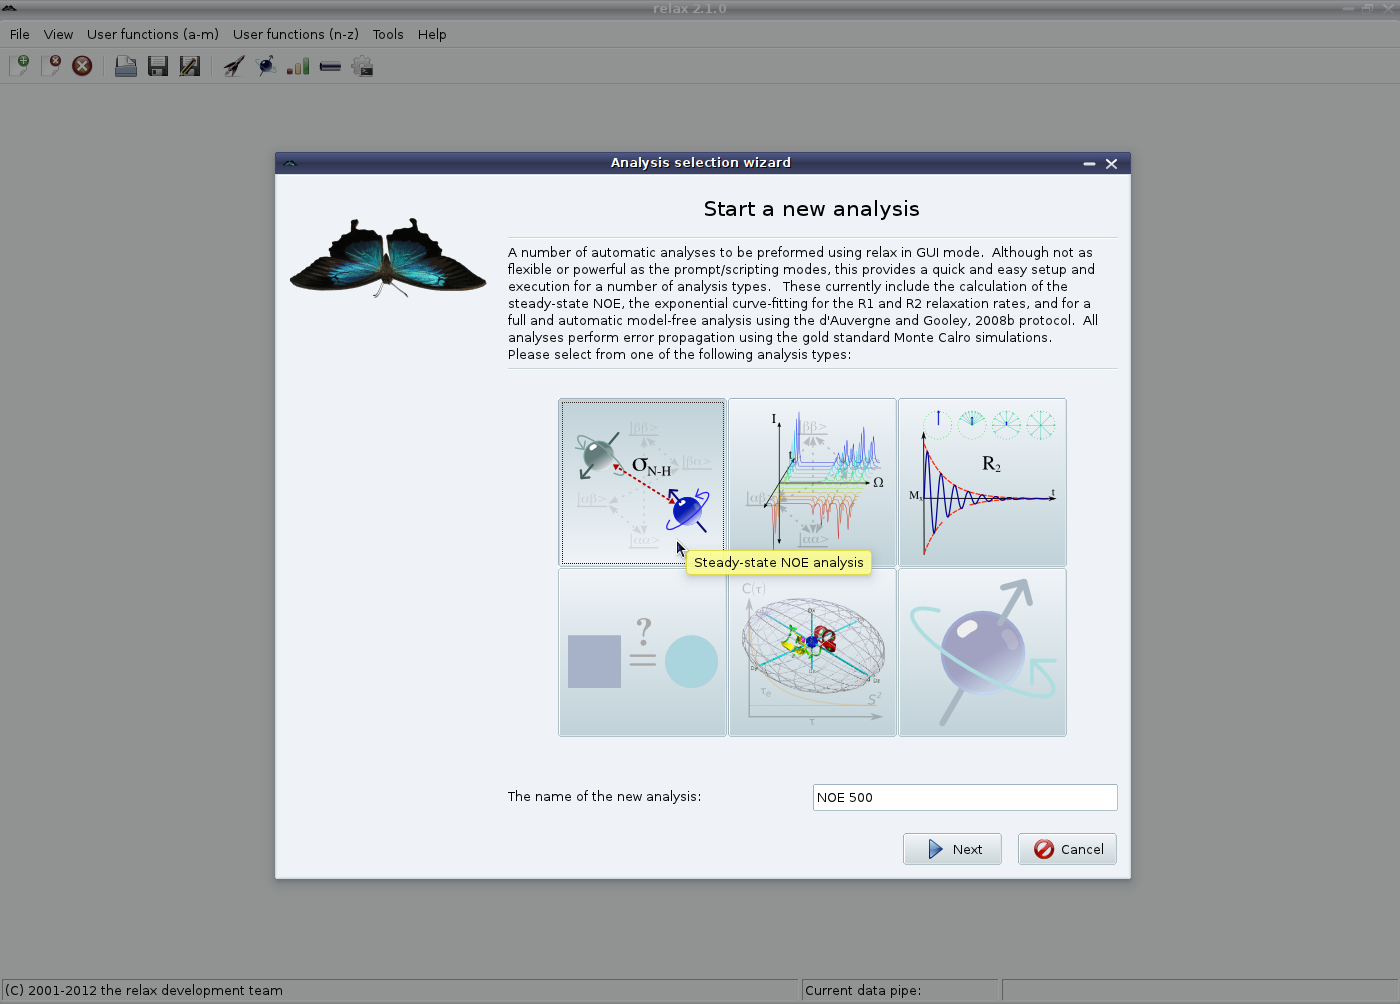
\includegraphics[
      width=0.8\textwidth,
      bb=14 14 1415 1019
    ]
    {graphics/screenshots/noe_analysis/analysis_wizard1}
  }
\end{minipage}

The second part of the wizard need not be modified, just click on \guibutton{Start} to begin.
This will create a dedicated data pipe for the analysis.
A data pipe bundle will also be created, but for the steady-state NOE will only contain a single data throughout the analysis.

\begin{minipage}[h]{\linewidth}
  \centerline{
    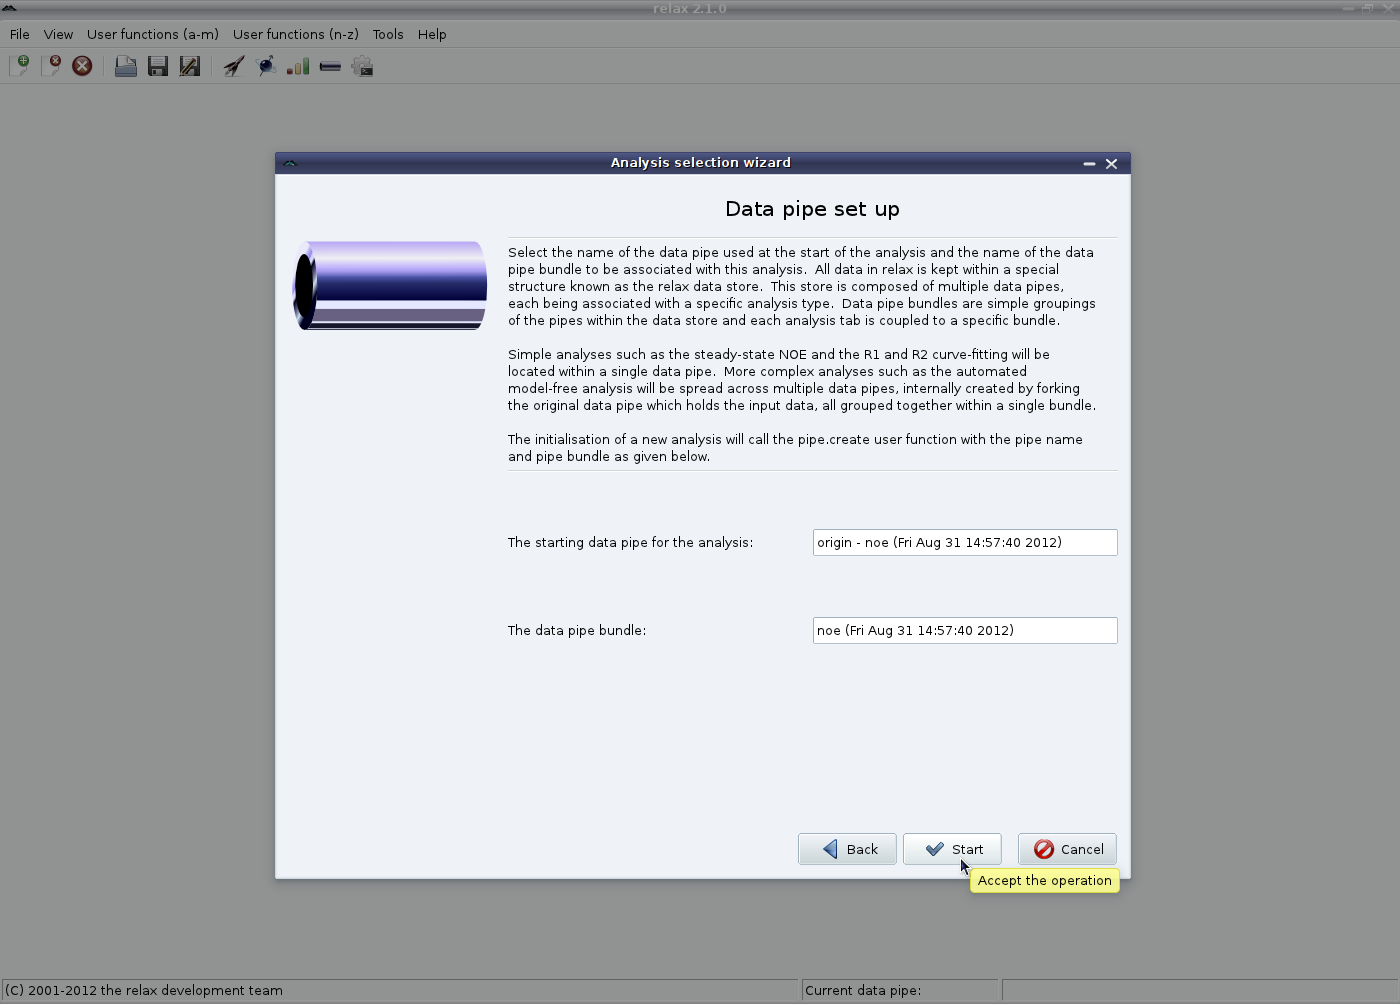
\includegraphics[
      width=0.8\textwidth,
      bb=14 14 1415 1019
    ]
    {graphics/screenshots/noe_analysis/analysis_wizard2}
  }
\end{minipage}


% General setup.
%~~~~~~~~~~~~~~~

\subsection{NOE GUI mode -- general setup}

You should then see the blank analysis tab:

\begin{minipage}[h]{\linewidth}
  \centerline{
    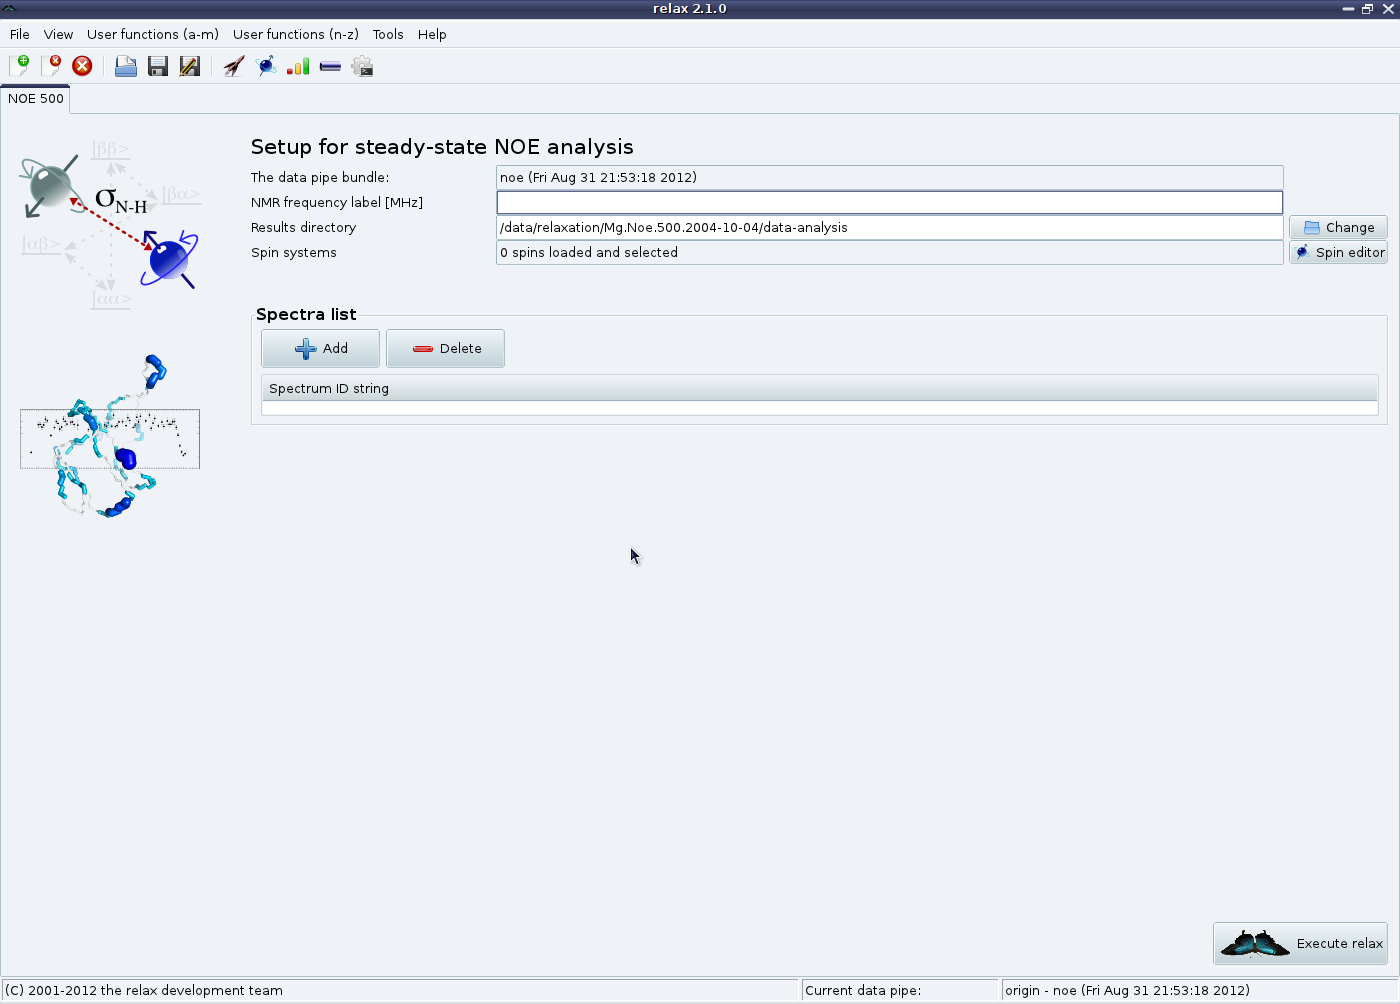
\includegraphics[
      width=0.8\textwidth,
      bb=14 14 1415 1019
    ]
    {graphics/screenshots/noe_analysis/blank}
  }
\end{minipage}

The first thing to do now is to set the NMR frequency label.
This is only used for the name of the NOE output file.
For example if you set the label to \guistring{500}, the file \file{noe.500.out} will be created at the end of the analysis.

You can also choose to change the \gui{Results directory} where all of the automatically created results files will be placed.
These two steps are unique to the GUI mode.


% Spin systems.
%~~~~~~~~~~~~~~

\subsection{NOE GUI mode -- setting up the spin systems}

Just as in the prompt and scripting UI modes, the molecule, residue and spin data structures need to be set up prior to the loading of any spin specific data.
The \gui{Spin systems} GUI element is used for this purpose.
Before any spin systems have been set up, this should say something like \gui{0 spins loaded and selected}.
To fix this, click on the \guibutton{Spin editor} button and you should then see the spin viewer window.
The next steps are fully described in section~\ref{sect: GUI - structural data} on page~\pageref{sect: GUI - structural data} for PDB files or section~\ref{sect: GUI - sequence file} on page~\pageref{sect: GUI - sequence file} for a sequence file.
The spin viewer window can now be closed.


% Unresolved spins.
%~~~~~~~~~~~~~~~~~~

\subsection{NOE GUI mode -- unresolved spins}

Using the unresolved spins file as described in the prompt/script UI sections, the same spins can be deselected at this point.
See Section~\ref{sect: GUI - deselect spins} on page~\pageref{sect: GUI - deselect spins} for the details of how to deselect the spins in the GUI.


% Loading the data.
%~~~~~~~~~~~~~~~~~~

\subsection{NOE GUI mode -- loading the data}

The next step is to load the saturated and reference NOE peak lists.
From the main NOE auto-analysis tab, click on the \guibutton{Add} button in the \gui{Spectra list} GUI element.
This will launch the NOE peak intensity loading wizard.
From the first wizard page, select the peak list file containing the reference intensities (from the averaged shift list):

\begin{minipage}[h]{\linewidth}
  \centerline{
    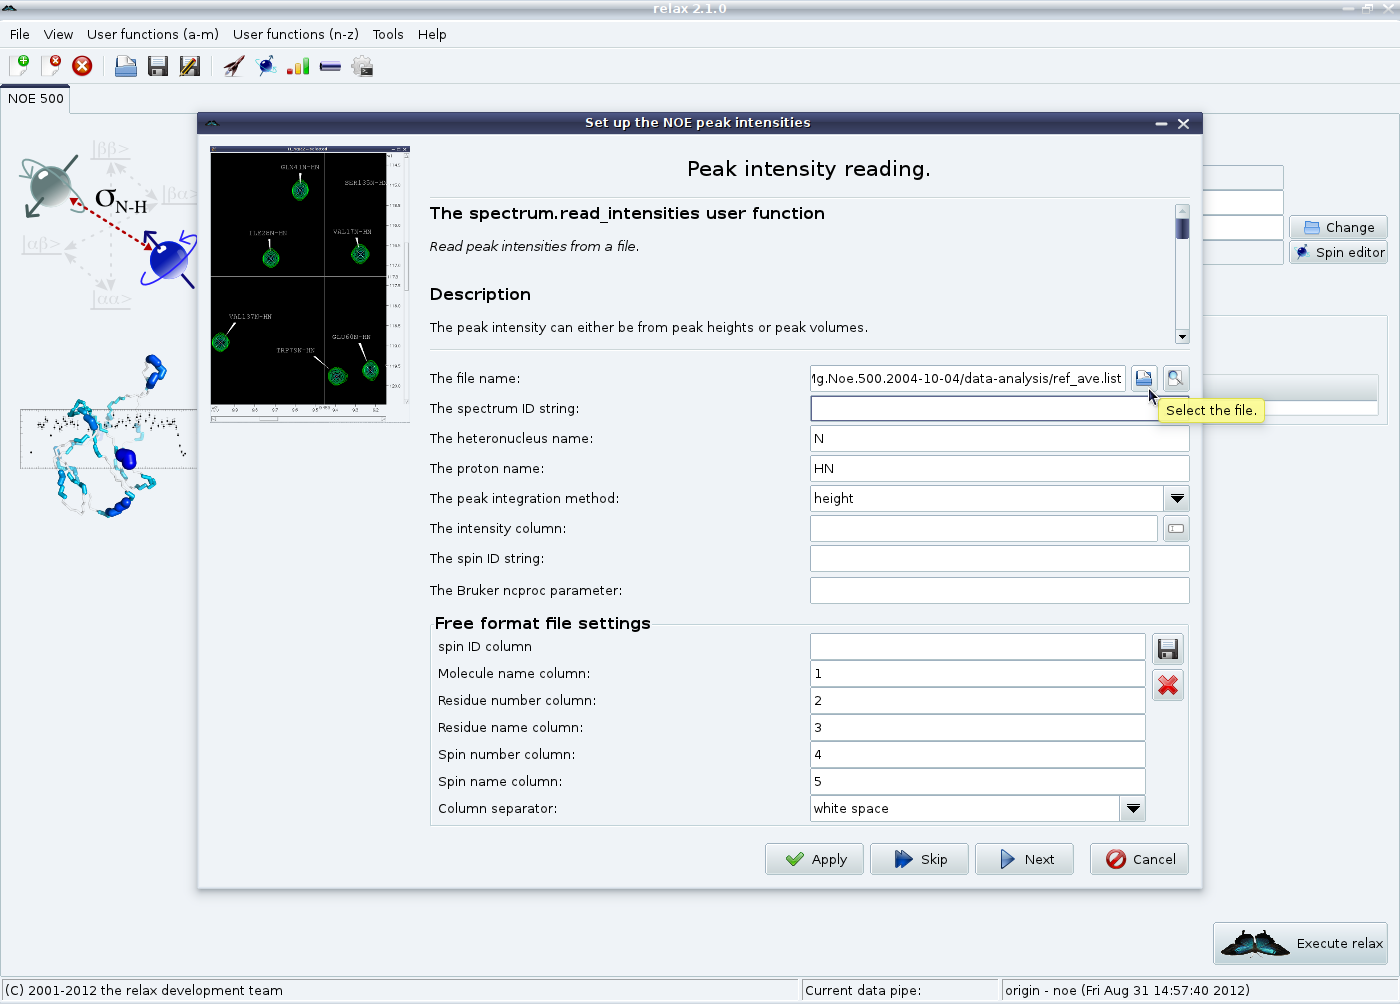
\includegraphics[
      width=0.8\textwidth,
      bb=14 14 1415 1019
    ]
    {graphics/screenshots/noe_analysis/peak_intensity1}
  }
\end{minipage}

Then set the obligatory spectrum ID string to a unique value (in this case \guistring{ref}).
The spectral dimension may need to be changed so that the peak intensities are associated with the correct atom of the pair.
In case you have forgotten the spin names or the format of the peak list next to the file name selection button is a preview button which can be used to open the peak list in the default text editor.
Set the other fields as needed.
Click on \guibutton{Next}
Note that a \prompt{RelaxWarning} will be thrown for all peak list entries which do not match a spin system within the relax data store.
This will cause the relax controller window to appear:

\begin{minipage}[h]{\linewidth}
  \centerline{
    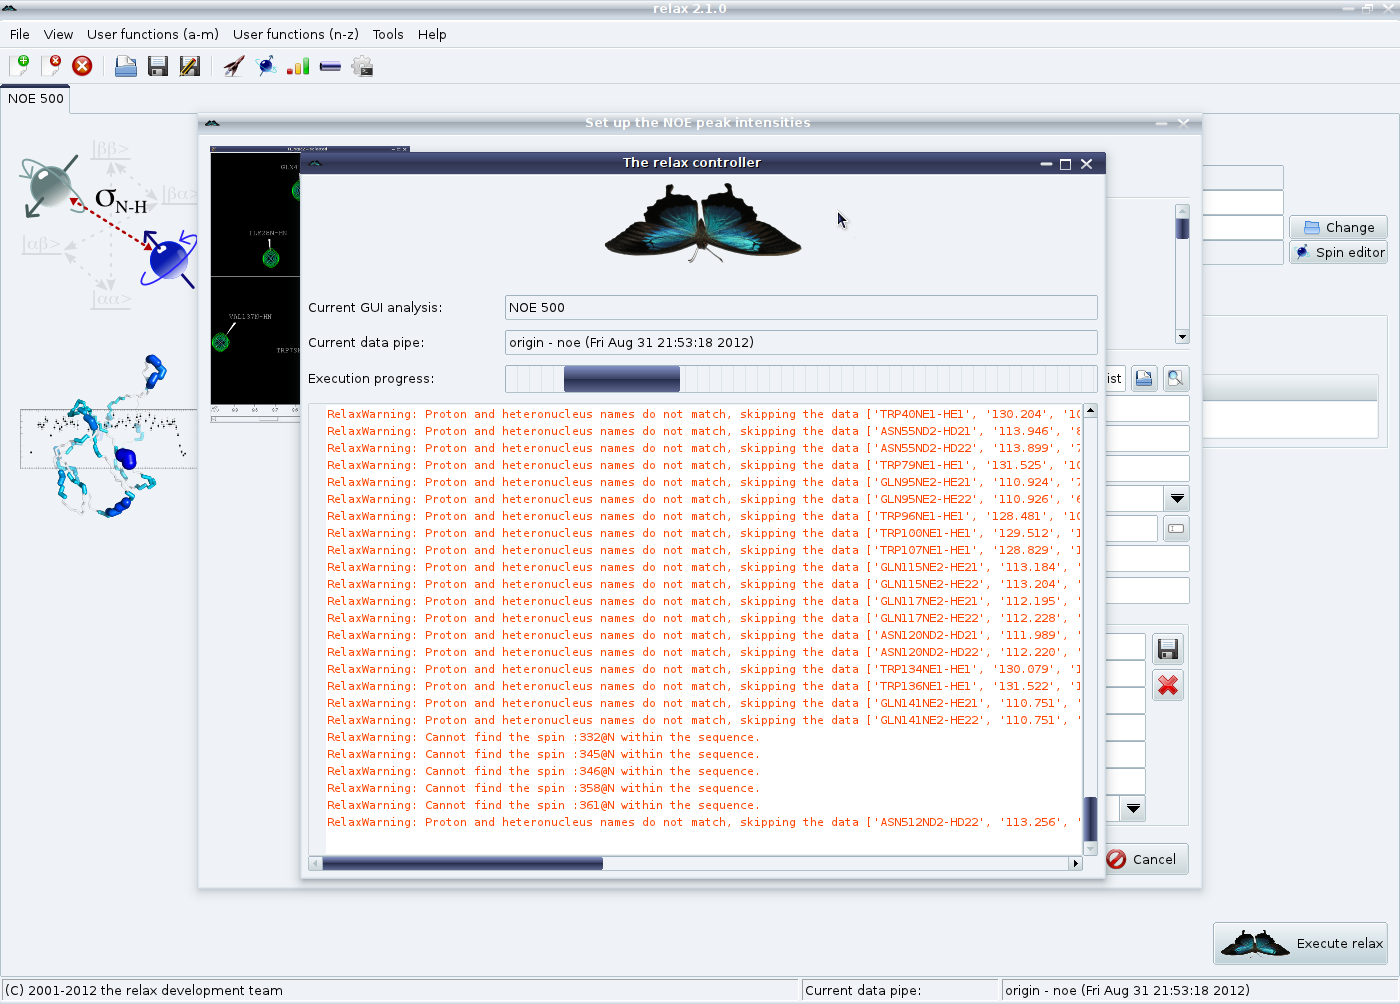
\includegraphics[
      width=0.8\textwidth,
      bb=14 14 1415 1019
    ]
    {graphics/screenshots/noe_analysis/peak_intensity2}
  }
\end{minipage}

Carefully check these warnings to be sure that the data is correctly loaded and, if everything is fine, the relax controller window can be closed.
If the dimension has been wrongly specified or some other setting is incorrect a \prompt{RelaxError} might appear saying that no data was loaded -- you will then need to fix the settings and click on \guibutton{Apply} again.
The error type page should now appear.

\begin{minipage}[h]{\linewidth}
  \centerline{
    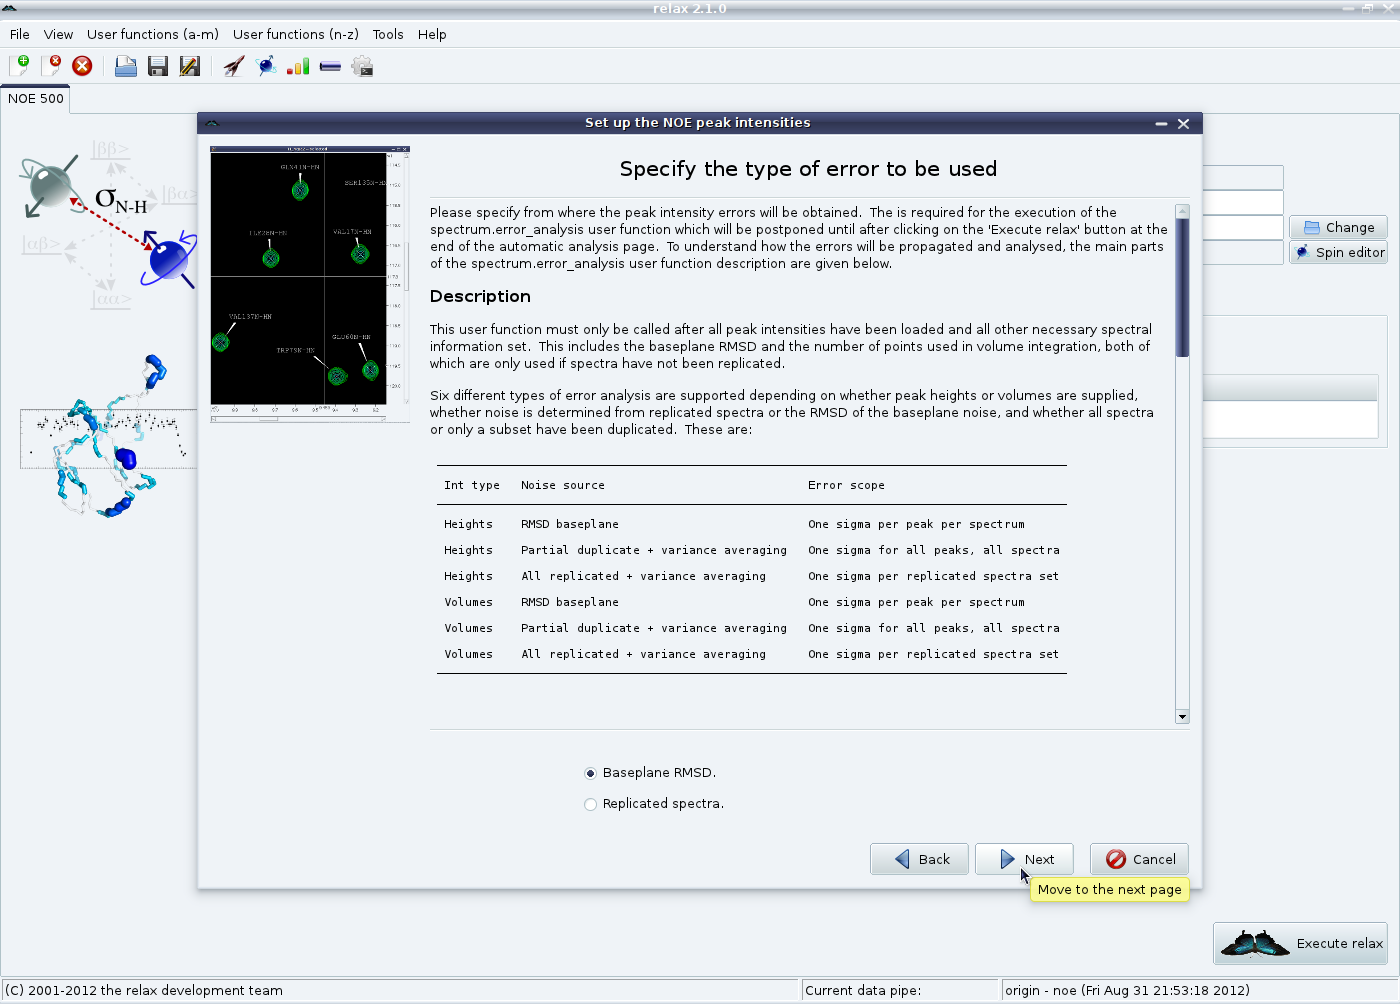
\includegraphics[
      width=0.8\textwidth,
      bb=14 14 1415 1019
    ]
    {graphics/screenshots/noe_analysis/peak_intensity4}
  }
\end{minipage}

Please read the description in this window very carefully to know what to do next.
In this example, we will choose \gui{Baseplane RMSD}.
For this specific example, Sparky's \guimenuitemthree{Extensions}{Spectrum}{Spectrum baseplane RMSD} option in the \gui{F1} selection mode was used to measure empty regions of the spectrum (mainly in the random coil region) to determine an average RMSD of approximately 3600.
Set the value and click on \guibutton{Apply}.

\begin{minipage}[h]{\linewidth}
  \centerline{
    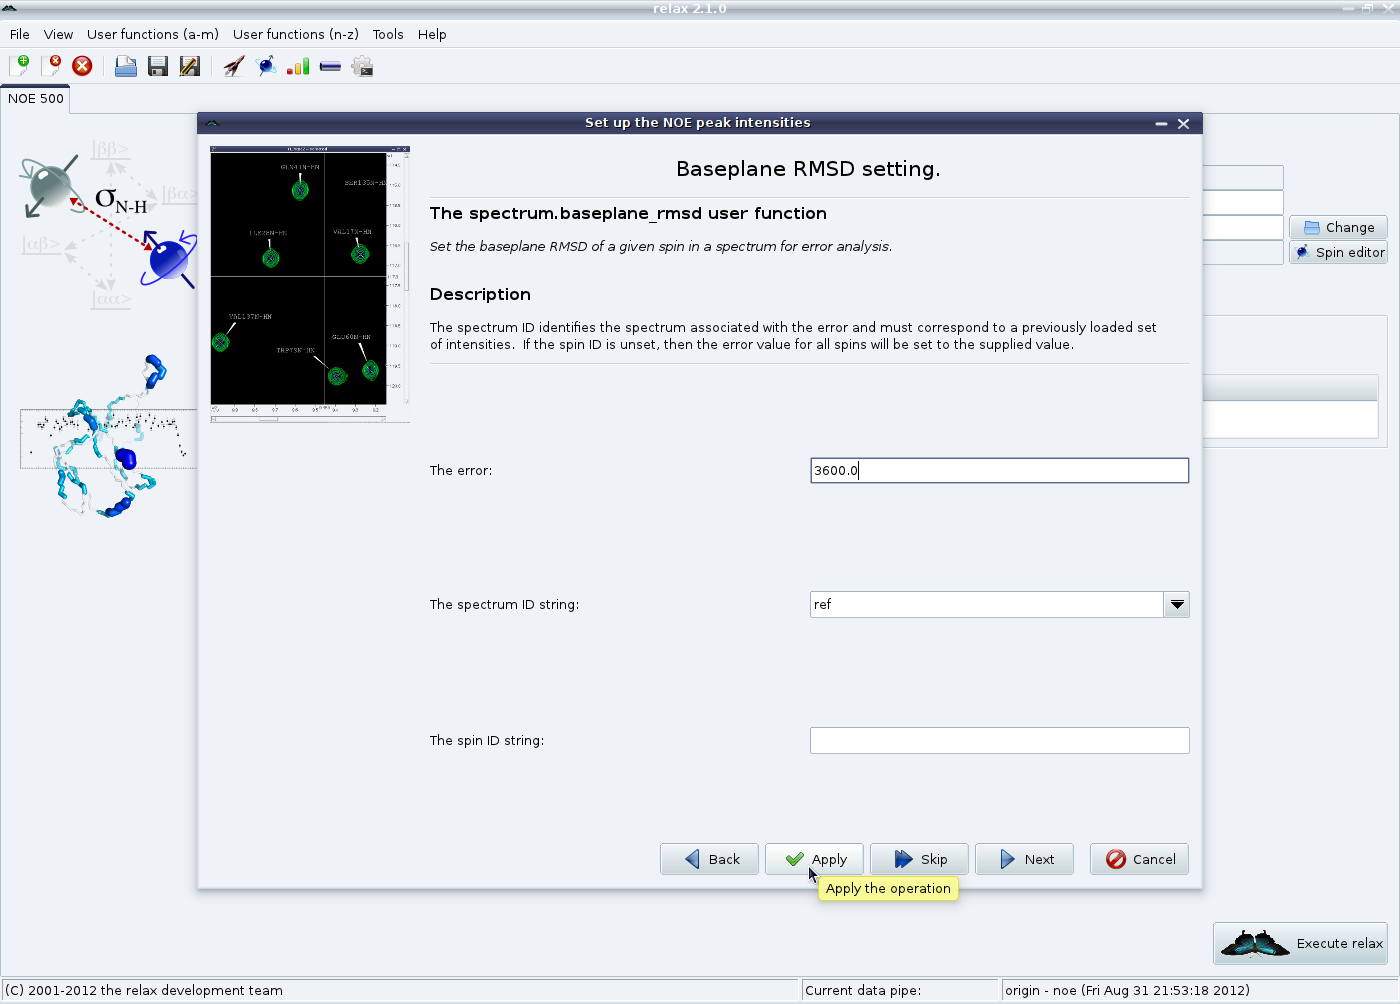
\includegraphics[
      width=0.8\textwidth,
      bb=14 14 1415 1019
    ]
    {graphics/screenshots/noe_analysis/peak_intensity5}
  }
\end{minipage}

As glycine 114 is located close to the noise signal, its error was much higher at 122000.
Individual spin errors can be set via the spin ID string (see section~\ref{sect: spin ID} on page~\pageref{sect: spin ID} for information about spin IDs):

\begin{minipage}[h]{\linewidth}
  \centerline{
    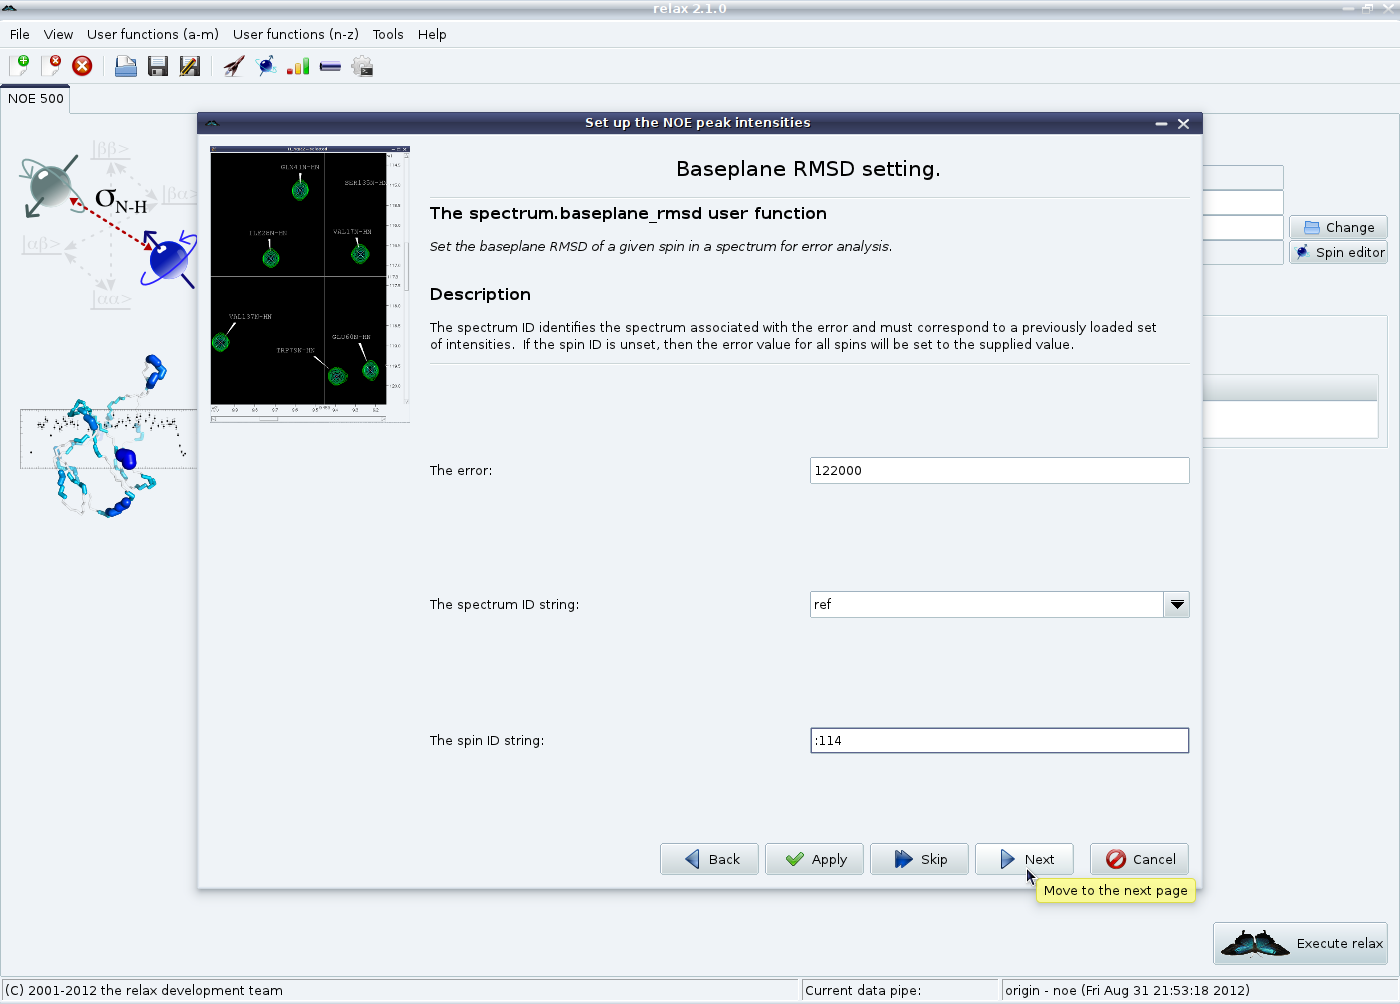
\includegraphics[
      width=0.8\textwidth,
      bb=14 14 1415 1019
    ]
    {graphics/screenshots/noe_analysis/peak_intensity6}
  }
\end{minipage}

Finally select which type of spectrum this is and click on \guibutton{Finish}:

\begin{minipage}[h]{\linewidth}
  \centerline{
    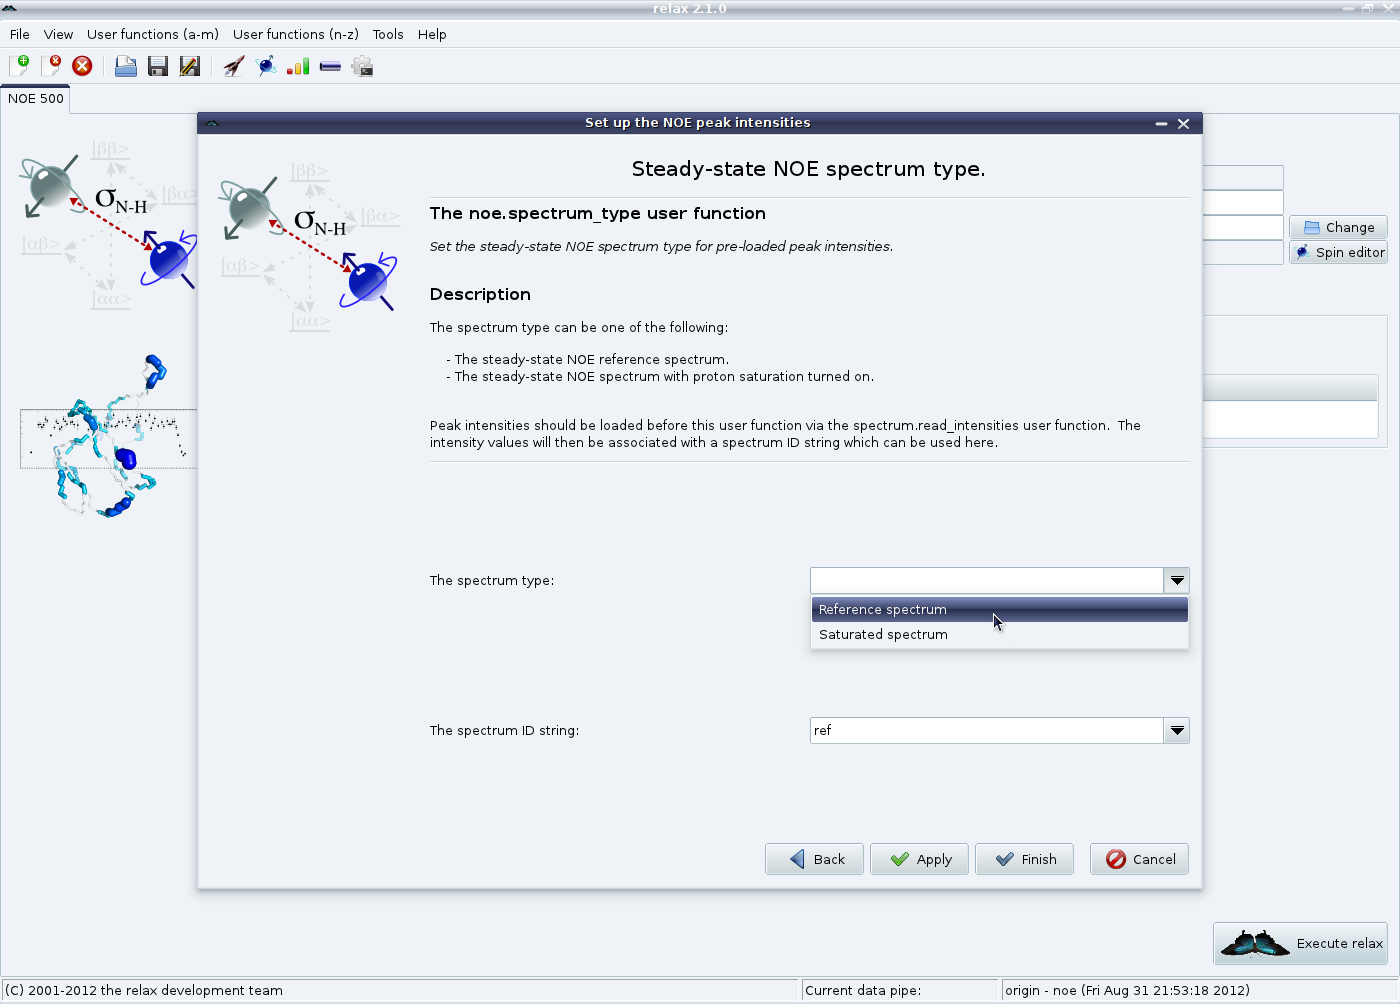
\includegraphics[
      width=0.8\textwidth,
      bb=14 14 1415 1019
    ]
    {graphics/screenshots/noe_analysis/peak_intensity7}
  }
\end{minipage}

The entire procedure should be repeated for the saturated spectrum (or you may have worked out that both can be loaded simultaneously by using the \guibutton{Apply} button more often).
For this example, the spectrum ID was set to \guistring{sat} and the baseplane RMSD to 3000 for all spins (except for G114 which had an error of 8500).

The NOE analysis tab should now look like:

\begin{minipage}[h]{\linewidth}
  \centerline{
    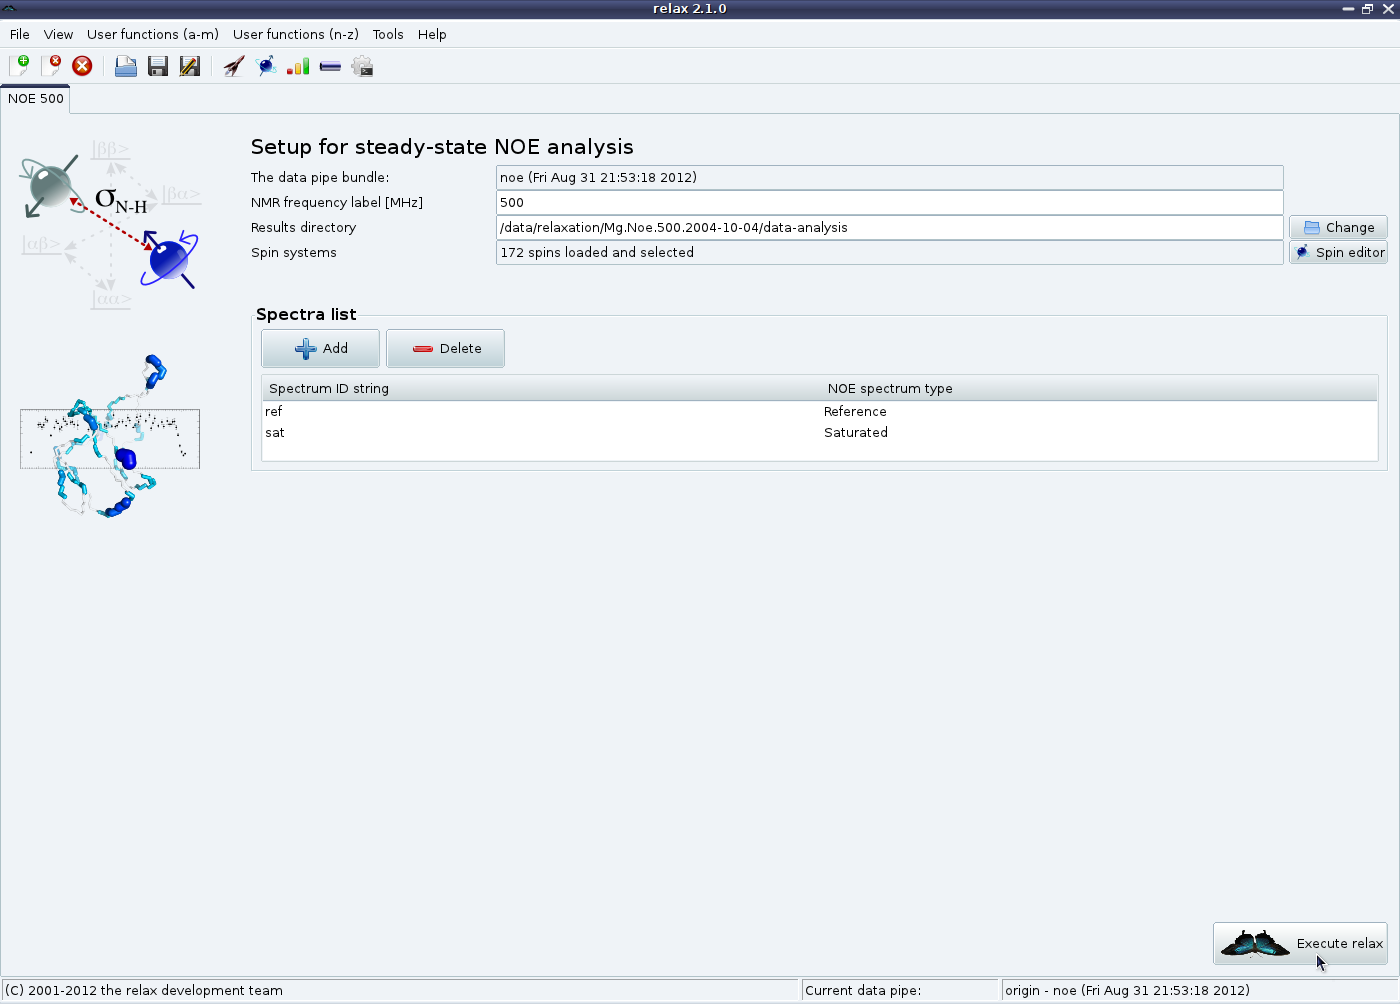
\includegraphics[
      width=0.8\textwidth,
      bb=14 14 1415 1019
    ]
    {graphics/screenshots/noe_analysis/analysis_tab2}
  }
\end{minipage}


% The NOE.
%~~~~~~~~~

\subsection{NOE GUI mode -- the NOE calculation}

Now that everything is set up, simply click on \guibutton{Execute relax} in the NOE analysis tab.
The relax controller window will appear displaying many messages.
These should all be checked very carefully to make sure that everything has executed as you expected.
The \gui{Results viewer} window will also appear:

\begin{minipage}[h]{\linewidth}
  \centerline{
    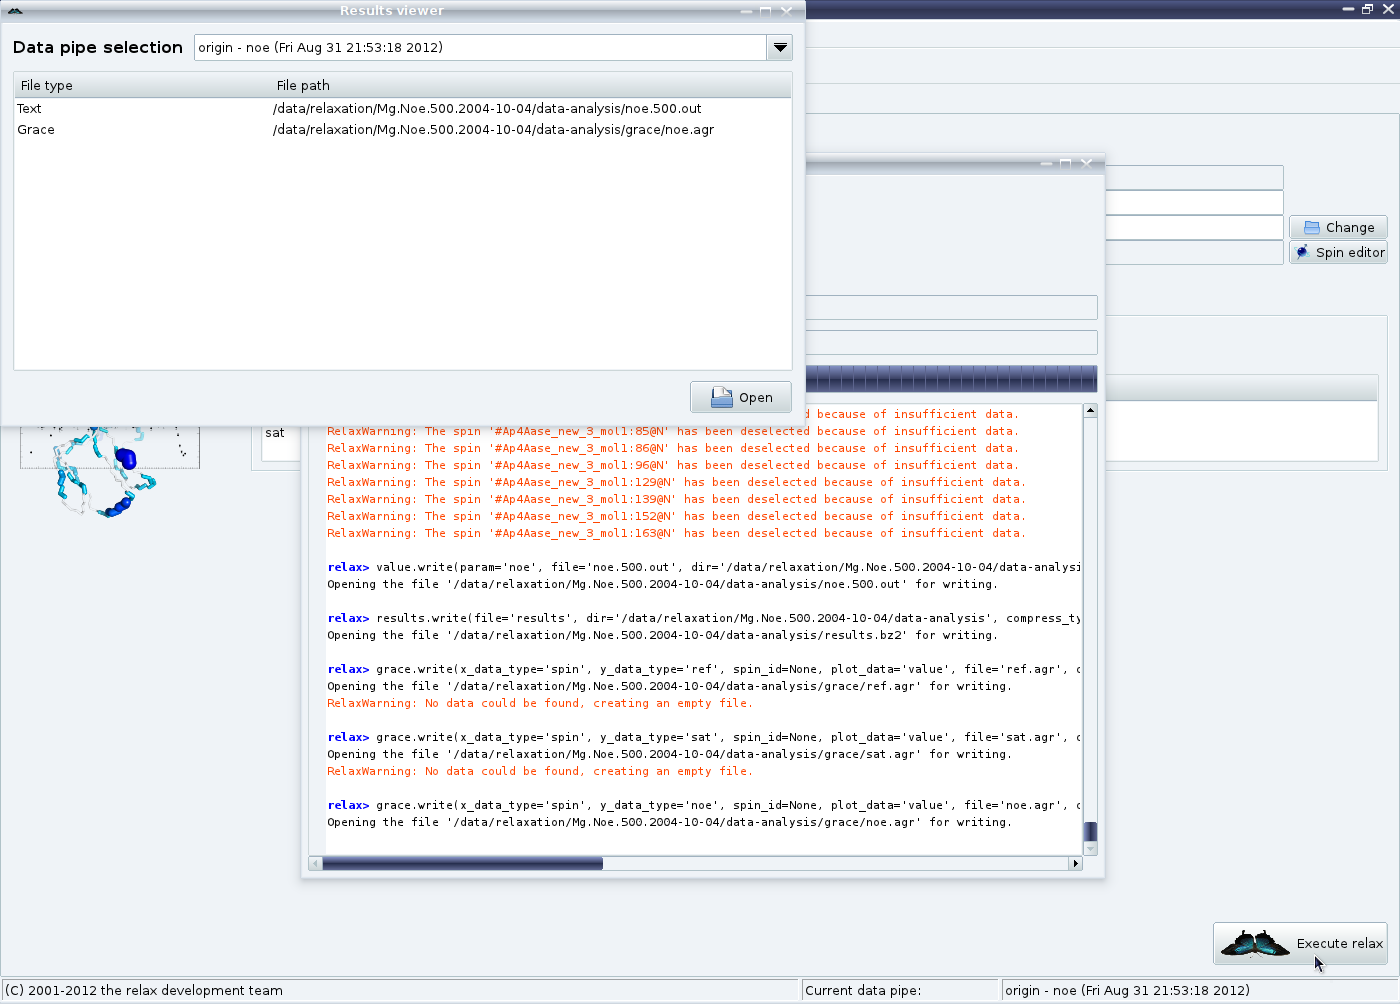
\includegraphics[
      width=0.8\textwidth,
      bb=14 14 1415 1019
    ]
    {graphics/screenshots/noe_analysis/fin}
  }
\end{minipage}

The results viewer window can be used to launch a text editor to see the NOE values and error or Grace to visualise the results (see Figure~\ref{fig: NOE plot} on page~\pageref{fig: NOE plot}).

As a last step, the relax state can be saved (via the \guimenuitemone{File} menu) and relax closed.
Take one last look at the \file{noe.out} log file to be certain that there are no strange warnings or errors.

% Relaxation curve-fitting.
%%%%%%%%%%%%%%%%%%%%%%%%%%%

\chapter[Relaxation curve-fitting]{The $\Rone$ and $\Rtwo$ relaxation rates -- relaxation curve-fitting} \label{ch: relax-fit}
\index{relaxation curve-fitting|textbf}


\begin{figure*}[h]
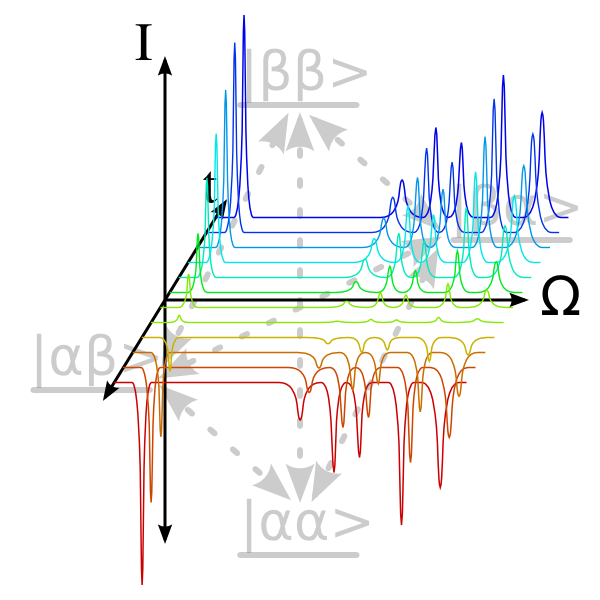
\includegraphics[width=5cm, bb=0 0 1701 1701]{graphics/analyses/r1_600x600} \hfill 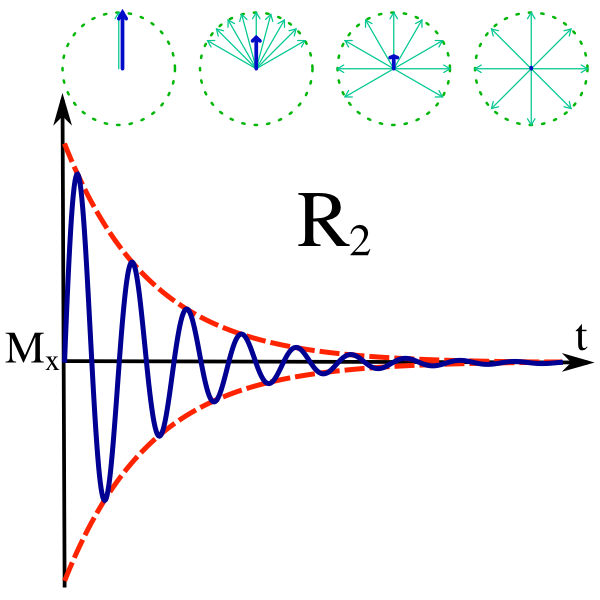
\includegraphics[width=5cm, bb=0 0 1701 1701]{graphics/analyses/r2_600x600}
\end{figure*}


% Introduction.
%%%%%%%%%%%%%%%

\section{Introduction to relaxation curve-fitting}

The fitting of exponentials to relaxation curves (relaxation curve-fitting or as used throughout this chapter abbreviated simply as relax-fit) involves a number of steps including the loading of data, the calculation of both the average peak intensity\index{peak!intensity} across replicated spectra and the standard deviations\index{standard deviation} of those peak intensities, selection of the experiment type, optimisation of the parameters of the exponential curves during the fit for each observed spin, Monte Carlo simulations\index{Monte Carlo simulation} to find the parameter errors, and saving and viewing the results.  To simplify the process a sample script will be followed step by step as was done with the NOE calculation.



% From spectra to peak intensities.
%%%%%%%%%%%%%%%%%%%%%%%%%%%%%%%%%%%

\section{From spectra to peak intensities for the relaxation rates} \label{sect: spectra to intensities}

The following subsections simply contain advice on how to go from the recorded FIDs to the peak lists ready to be input into relax.  This need not be followed -- it is simply a set of recommendations for obtaining the highest quality relaxation rates.


% Temperature control and calibration.
%~~~~~~~~~~~~~~~~~~~~~~~~~~~~~~~~~~~~~

\subsection{Temperature control and calibration} \label{sect: temperature control and calibration}


\includegraphics[bb=0 0 18 18]{/data/relax/relax-trunk/graphics/oxygen_icons/128x128/status/weather-clear}

Before starting with the spectral processing, it should be noted that proper temperature control and calibration are essential for relaxation data.  Small temperature changes can have an effect on the viscosity and hence global tumbling of the molecule being studied and, as the molecular diffusion tensor is the major contributor to relaxation, any non-consistent data will likely lead to artificial motions appearing in subsequent model-free analyses.

Per-experiment temperature calibration is essential and the technique used will need to be specified for BMRB data deposition.  Note that the standard MeOH/ethylene glycol calibration of a spectrometer is of no use when you are running experiments which pump in large amounts of power into the probe head.  Although the R1 experiment should be about the same temperature as a HSQC and hence be close to the standard MeOH/ethylene glycol spectrometer calibration, the R2 CPMG or spin lock and, to a lesser extent, the NOE pre-saturation pump a lot more power into the probe head.  The power differences can either cause the temperature in the sample to be too high or too low.  This is unpredictable as the thermometer used by the VT unit is next to the coils in the probe head and not inside the NMR sample.  So the VT unit tries to control the temperature inside the probe head rather than in the NMR sample.  However between the thermometer and the sample is the water of the sample, the glass of the NMR tube, the air gap where the VT unit controls air flow and the outside components of the probe head protecting the electronics.  If the sample, the probe head or the VT unit is changed, this will have a different affect on the per-experiment temperature.  The VT unit responds differently under different conditions and may sometimes over or under compensate by a couple of degrees.  Therefore each relaxation data set from each spectrometer requires a per-experiment calibration.

Explicit temperature control techniques are also essential for relaxation data collection.  Again the technique used will be asked for by relax for BMRB data deposition.  A number of factors can cause significant temperature fluctuations between individual relaxation experiments.  This includes the daily temperature cycle of the room housing the spectrometer, different amounts of power for the individual experiments, etc.  The best methods for eliminating such problems are single scan interleaving and temperature compensation block.  Single scan interleaving is the most powerful technique for averaging the temperature fluctuations not only across different experiments, but also across the entire measurement time.  The application of off-resonance temperature compensation blocks at the start of the experiment is useful for the R2 and will normalise the temperature between the individual experiments, but single scan or single fid interleaving is nevertheless required for normalising the temperature across the entire measurement.


% Spectral processing.
%~~~~~~~~~~~~~~~~~~~~~

\subsection{Spectral processing}

For the best measurement of peak heights across the myriad of NMR spectral analysis softwares, it is recommend to zero fill a lot -- 8k to 16k would give the best results.  This does not increase the information content of the spectrum or decrease the errors, it simply interpolates.  Even if the NMR spectral software performs 3-point quadratic interpolation between the highest points to determine the peak height, the additional free interpolation will make the estimation more accurate.

Additionally, care must be taken to properly scale the first point as this can cause a baseline roll which will affect peak heights.  A very useful description comes directly from the \href{http://spin.niddk.nih.gov/NMRPipe/doc1/}{NMRPipe manual}:

\begin{quotation}
Depending on the delay, the first point of the FID should be adjusted before Fourier Transform.  The first point scaling factor is selected by the window function argument \prompt{-c}.

If the required first order phase P1 for the given dimension is 0.0, the first point scaling factor should be 0.5.  This is because the discrete Fourier transform does the equivalent of counting the point at t=0 twice.  If the first point is not scaled properly in this case, ridge-line baseline offsets in the spectrum will result.

In all other cases (P1 is not zero), this scale factor should be 1.0. This is because the first point of the FID no longer corresponds to t=0, and so it shouldn't be scaled. If the scale factor is not set correctly, it will introduce a baseline distortion which is either zero-order or sinusoidal, depending on what first-order phase is required. When possible, it is best to set up experiments with either exactly 0, 1/2, or 1-point delay.  There are several reasons:

\begin{itemize}
\item Phase correction values can be determined easily.
\item If the delay is not a multiple of 1/2 point, the phase of folded peaks will be distorted.
\item The Hilbert transform (HT) is used, sometimes automatically, to reconstruct previously deleted imaginary data for interactive rephasing or inverse processing. But, the HT can only reconstruct imaginary data perfectly if the phase is a multiple of 1/2 point.
\item Data with P1 = 360 have the first point t=0 missing (i.e. 1 point delay). Since the first point of the FID corresponds to the sum of points in the corresponding spectrum, this missing first point can be ``restored'' by adding a constant to the phased spectrum.  This can be done conveniently by automated zero-order baseline correction, as shown in table~\ref{table: NMRPipe -c}.

\begin{table}
\begin{center}
\caption{Summary, First Point Scaling and Phase Correction}
\begin{tabular}{llll}
\toprule
Delay & P1 & FID & Spectrum\\
\midrule
0   point &   0 & Scale -c 0.5 \\
1/2 point & 180 & Scale -c 1.0 & Folded peaks have opposite sign \\
1   point & 360 & Scale -c 1.0 & Use ``POLY -auto -ord 0'' \\
\bottomrule
\label{table: NMRPipe -c}
\end{tabular}
\end{center}
\end{table}

\end{itemize}
\end{quotation}


Here is an example NMRPipe script designed for optimal relaxation rate extraction:

\begin{exampleenv}
\#!/bin/csh \\
 \\
setenv FILEROOT \$1 \\
set PHASE=81.4 \\
 \\
echo "\textbackslash n\# Fourier Transform (nmrPipe fid/*.fid to ft/*.dat)" \\
echo "\# t2 phase is set to \$PHASE" \\
echo "\# t1 phase is set to 0.0\textbackslash n" \\
 \\
nmrPipe -in fid/\$FILEROOT.fid \ \\
| nmrPipe -fn SOL \ \\
| nmrPipe -fn GM -g1 15 -g2 20 -c 0.5 \ \\
| nmrPipe -fn ZF -size 8192 \ \\
| nmrPipe -fn FT -auto \ \\
| nmrPipe -fn PS -p0 \$PHASE -p1 0.0 -di -verb \ \\
| nmrPipe -fn EXT -left -sw \ \\
| nmrPipe -fn TP \ \\
| nmrPipe -fn SP -off 0.5 -end 0.98 -pow 2 -c 0.5 \ \\
| nmrPipe -fn ZF -size 8192 \ \\
| nmrPipe -fn FT -auto \ \\
| nmrPipe -fn PS -p0 0.0 -p1 0.0 -di -verb \ \\
| nmrPipe -fn REV \ \\
| nmrPipe -fn TP \ \\
| nmrPipe -out ft/\$FILEROOT.dat -ov
\end{exampleenv}


% Measuring peak intensities.
%~~~~~~~~~~~~~~~~~~~~~~~~~~~~

\subsection{Measuring peak intensities}

For the measurement of peak intensities, again care must be taken.  A read of the paper:

\begin{itemize}
\item \bibentry{Viles01}
\end{itemize}

is highly recommended.  Despite the recommendations in the discussion of this paper, a different methodology using peak heights can be used to solve the same problems.  This will be discussed in a paper which is currently in preparation from the Gooley group.  The steps involved are:

\begin{itemize}
\item For the first spectrum in the time series, shift the peak list to the tops of the peaks (for example using \gui{pc} in Sparky on subsets of peaks).
\item Copy this \nth{1} spectrum list onto all spectra, shifting the peaks to the top as in the previous step.
\item When the peak disappears into the noise, leave it at its current position and do not type \gui{pc} or equivalent.  This will add weight to the first point in the subsequent step.
\item Once all spectra are shifted, calculate an average peak list.
\item Copy this average peak list onto fresh copies of all spectra.
\item Measure peak heights using this averaged peak list.
\end{itemize}

This will produce the most accurate peak intensity measurements until better, more robust peak shape integration comes along.  This is a special technique which is designed to minimise the white-noise bias talked about in the \citet{Viles01} paper.  As the noise often decreases with the decrease in total spectral power, using the tops of the peaks means that you are actually measuring the real peak height plus positive noise in all cases.  This non-constant additional positive noise contribution can result in a double exponential in the measured data.  The technique above eliminates this as you then measure close to real peak height with the addition of white noise centred at zero -- it is both negative and positive to equal amounts -- rather than the peak high with noise contribution strongly biased towards the positive.  Where the peaks disappear, you then are measuring the pure baseplane noise.  This is fine as these white-noise data points centred at zero will help in the subsequent exponential fit in relax. 

If using Sparky then, to be sure that the peak heights are properly updated, for each spectrum type \gui{pa} to select all peaks, \gui{ph} to update all selected peak heights, \gui{lt} to show the spectrum peaks window, make sure \gui{data height} is selected in the options, and then save the peak list.



% Script UI.
%%%%%%%%%%%%
\section{Relaxation curve-fitting in the prompt/script UI mode}


% The sample script.
%~~~~~~~~~~~~~~~~~~~

\subsection{Relax-fit script mode -- the sample script}

The following is a verbatim copy of the contents of the \file{sample\_scripts/relax\_fit.py} file.  If your copy of the sample script is different than that below, please send an email to the relax-devel mailing list\index{mailing list!relax-devel} to tell the relax developers that the manual is out of date (see section~\ref{sect: relax-devel mailing list} on page~\pageref{sect: relax-devel mailing list}).  You will need to first copy this script to a dedicated analysis directory containing peak lists, a PDB file and a file listing unresolved spin systems, and then modify its contents to suit your specific analysis.  The script contents are:

\begin{exampleenv}
\# Script for relaxation curve-fitting. \\
 \\
\# Create the `rx' data pipe. \\
pipe.create(`rx', `relax\_fit') \\
 \\
\# Load the backbone amide 15N spins from a PDB file. \\
structure.read\_pdb(`Ap4Aase\_new\_3.pdb') \\
structure.load\_spins(spin\_id=`@N') \\
 \\
\# Spectrum names. \\
names = [ \\
\hspace*{4ex} `T2\_ncyc1\_ave', \\
\hspace*{4ex} `T2\_ncyc1b\_ave', \\
\hspace*{4ex} `T2\_ncyc2\_ave', \\
\hspace*{4ex} `T2\_ncyc4\_ave', \\
\hspace*{4ex} `T2\_ncyc4b\_ave', \\
\hspace*{4ex} `T2\_ncyc6\_ave', \\
\hspace*{4ex} `T2\_ncyc9\_ave', \\
\hspace*{4ex} `T2\_ncyc9b\_ave', \\
\hspace*{4ex} `T2\_ncyc11\_ave', \\
\hspace*{4ex} `T2\_ncyc11b\_ave' \\
] \\
 \\
\# Relaxation times (in seconds). \\
times = [ \\
\hspace*{4ex} 0.0176, \\
\hspace*{4ex} 0.0176, \\
\hspace*{4ex} 0.0352, \\
\hspace*{4ex} 0.0704, \\
\hspace*{4ex} 0.0704, \\
\hspace*{4ex} 0.1056, \\
\hspace*{4ex} 0.1584, \\
\hspace*{4ex} 0.1584, \\
\hspace*{4ex} 0.1936, \\
\hspace*{4ex} 0.1936 \\
] \\
 \\
\# Loop over the spectra. \\
for i in xrange(len(names)): \\
\hspace*{4ex} \# Load the peak intensities. \\
\hspace*{4ex} spectrum.read\_intensities(file=names[i]+`.list', dir=data\_path, spectrum\_id=names[i], int\_method=`height') \\
 \\
\hspace*{4ex} \# Set the relaxation times. \\
\hspace*{4ex} relax\_fit.relax\_time(time=times[i], spectrum\_id=names[i]) \\
 \\
\# Specify the duplicated spectra. \\
spectrum.replicated(spectrum\_ids=[`T2\_ncyc1\_ave', `T2\_ncyc1b\_ave']) \\
spectrum.replicated(spectrum\_ids=[`T2\_ncyc4\_ave', `T2\_ncyc4b\_ave']) \\
spectrum.replicated(spectrum\_ids=[`T2\_ncyc9\_ave', `T2\_ncyc9b\_ave']) \\
spectrum.replicated(spectrum\_ids=[`T2\_ncyc11\_ave', `T2\_ncyc11b\_ave']) \\
 \\
\# Peak intensity error analysis. \\
spectrum.error\_analysis() \\
 \\
\# Deselect unresolved spins. \\
deselect.read(file=`unresolved', mol\_name\_col=1, res\_num\_col=2, res\_name\_col=3, spin\_num\_col=4, spin\_name\_col=5) \\
 \\
\# Set the relaxation curve type. \\
relax\_fit.select\_model(`exp') \\
 \\
\# Grid search. \\
grid\_search(inc=11) \\
 \\
\# Minimise. \\
minimise(`simplex', scaling=False, constraints=False) \\
 \\
\# Monte Carlo simulations. \\
monte\_carlo.setup(number=500) \\
monte\_carlo.create\_data() \\
monte\_carlo.initial\_values() \\
minimise(`simplex', scaling=False, constraints=False) \\
monte\_carlo.error\_analysis() \\
 \\
\# Save the relaxation rates. \\
value.write(param=`rx', file=`rx.out', force=True) \\
 \\
\# Save the results. \\
results.write(file=`results', force=True) \\
 \\
\# Create Grace plots of the data. \\
grace.write(y\_data\_type=`chi2', file=`chi2.agr', force=True)    \# Minimised chi-squared value. \\
grace.write(y\_data\_type=`i0', file=`i0.agr', force=True)    \# Initial peak intensity. \\
grace.write(y\_data\_type=`rx', file=`rx.agr', force=True)    \# Relaxation rate. \\
grace.write(x\_data\_type=`relax\_times', y\_data\_type=`intensities', file=`intensities.agr', force=True)    \# Average peak intensities. \\
grace.write(x\_data\_type=`relax\_times', y\_data\_type=`intensities', norm=True, file=`intensities\_norm.agr', force=True)    \# Average peak intensities (normalised). \\
 \\
\# Display the Grace plots. \\
grace.view(file=`chi2.agr') \\
grace.view(file=`i0.agr') \\
grace.view(file=`rx.agr') \\
grace.view(file=`intensities.agr') \\
grace.view(file=`intensities\_norm.agr') \\
 \\
\# Save the program state. \\
state.save(`rx.save', force=True)
\end{exampleenv}

The next sections will break this script down into its logical components and explain how these parts will be interpreted by relax.  To execute this script, please see section~\ref{sect: scripting} on page~\pageref{sect: scripting} for details.


% Initialisation of the data pipe.
%~~~~~~~~~~~~~~~~~~~~~~~~~~~~~~~~~

\subsection{Relax-fit script mode -- initialisation of the data pipe} \label{Rx initialisation}

The data pipe is simply created by the command

\example{pipe.create(`rx', `relax\_fit')}

This user function will then create a relaxation exponential curve-fitting specific data pipe labelled \promptstring{rx}.  The second argument sets the pipe type to that of the relaxation curve-fitting.  Setting the pipe type is important so that the program knows which user functions are compatible with the data pipe, for example in the steady-state NOE analysis the function \uf{minimise} (see page~\pageref{uf: minimise}) is meaningless as the NOE values are calculated directly rather than optimised.


% Spin systems.
%~~~~~~~~~~~~~~

\subsection{Relax-fit script mode -- setting up the spin systems}

The first thing which need to be completed prior to any spin specific command is to generate the molecule, residue and spin data structures for storing the spin specific data.  In the sample script above this is generated from a PDB file, however a plain text file with the sequence information can be used instead (see the \uf{sequence.read} user function on page~\pageref{uf: sequence.read} for more details).  In the case of the sample script, the command

\example{structure.read\_pdb(name, `Ap4Aase\_new\_3.pdb')}
\index{PDB}

will load the PDB file \file{Ap4Aase\_new\_3.pdb} into relax.  Then 

\begin{exampleenv}
structure.load\_spins(spin\_id=`@N') \\
structure.load\_spins(spin\_id=`@NE1')
\end{exampleenv}

will generate the molecule, residue, and spin sequence for the current data pipe.  In this situation there will be a single spin system per residue generated corresponding to the backbone amide nitrogens as well as $^{15}$N spins set up for the tryptophan indole nitrogens.  Although the 3D coordinates have been loaded into the program from the PDB file, this structural information serves no purpose when calculating $\Rone$ and $\Rtwo$ values.


% Loading the data.
%~~~~~~~~~~~~~~~~~~

\subsection{Relax-fit script mode -- loading the data}

To load the peak intensities\index{peak!intensity} into relax the user function \uf{spectrum.read\_intensities} is executed.  Important keyword arguments to this command are the file name and directory, the spectrum identification string and the relaxation time period of the experiment in seconds.  By default the file format will be automatically detected.  Currently Sparky\index{software!Sparky}, XEasy\index{software!XEasy}, NMRView\index{software!NMRView}, and generic columnar formatted peak lists are supported.  To be able to import any other type of format please send an email to the relax development mailing list\index{mailing list!relax-devel} with the details of the format.  Adding support for new formats is trivial.  The following series of commands -- an expansion of the \prompt{for} loop in the sample script -- will load peak intensities from six different relaxation periods, four of which have been duplicated, from Sparky peak lists with the peak heights in the 10$^\textrm{th}$ column.

\begin{exampleenv}
spectrum.read\_intensities(`T2\_ncyc1.list',   spectrum\_id=`1',   relax\_time=0.0176, int\_col=10) \\
spectrum.read\_intensities(`T2\_ncyc1b.list',  spectrum\_id=`1b',  relax\_time=0.0176, int\_col=10) \\
spectrum.read\_intensities(`T2\_ncyc2.list',   spectrum\_id=`2',   relax\_time=0.0352, int\_col=10) \\
spectrum.read\_intensities(`T2\_ncyc4.list',   spectrum\_id=`4',   relax\_time=0.0704, int\_col=10) \\
spectrum.read\_intensities(`T2\_ncyc4b.list',  spectrum\_id=`4b',  relax\_time=0.0704, int\_col=10) \\
spectrum.read\_intensities(`T2\_ncyc6.list',   spectrum\_id=`6',   relax\_time=0.1056, int\_col=10) \\
spectrum.read\_intensities(`T2\_ncyc9.list',   spectrum\_id=`9',   relax\_time=0.1584, int\_col=10) \\
spectrum.read\_intensities(`T2\_ncyc9b.list',  spectrum\_id=`9b',  relax\_time=0.1584, int\_col=10) \\
spectrum.read\_intensities(`T2\_ncyc11.list',  spectrum\_id=`11',  relax\_time=0.1936, int\_col=10) \\
spectrum.read\_intensities(`T2\_ncyc11b.list', spectrum\_id=`11b', relax\_time=0.1936, int\_col=10) \\
 \\
spectrum.replicated(spectrum\_ids=[`T2\_ncyc1\_ave', `T2\_ncyc1b\_ave']) \\
spectrum.replicated(spectrum\_ids=[`T2\_ncyc4\_ave', `T2\_ncyc4b\_ave']) \\
spectrum.replicated(spectrum\_ids=[`T2\_ncyc9\_ave', `T2\_ncyc9b\_ave']) \\
spectrum.replicated(spectrum\_ids=[`T2\_ncyc11\_ave', `T2\_ncyc11b\_ave'])
\end{exampleenv}

Note that the relaxation time period should be calculated directly from the pulse sequence (as the sum of delays and pulses for the peroid), as the estimated time may not match the real time.   For the Sparky peak lists, by default relax assumes that the intensity value is in the 4$^\textrm{th}$ column.  A typical file looks like:

{\scriptsize \begin{verbatim}
     Assignment         w1         w2   Data Height

        LEU3N-HN    122.454      8.397       129722
        GLY4N-HN    111.999      8.719       422375
        SER5N-HN    115.085      8.176       384180
        MET6N-HN    120.934      8.812       272100
        ASP7N-HN    122.394      8.750       174970
        SER8N-HN    113.916      7.836       218762
       GLU11N-HN    122.194      8.604        30412
       GLY12N-HN    110.525      9.028        90144
\end{verbatim}}

By supplying the \keyword{int\_col} argument to the \uf{spectrum.read\_intensities} user function, this can be changed.  A typical XEasy file will look like:

{\scriptsize \begin{verbatim}
 No.  Color    w1      w2     ass. in w1     ass. in w2    Volume     Vol. Err.  Method  Comment

   2    2    10.014 134.221   HN  21 LEU      N  21 LEU    7.919e+03  0.00e+00     m
   3    2    10.481 132.592  HE1  79 TRP    NE1  79 TRP    1.532e+04  0.00e+00     m
  17    2     9.882 129.041   HN 110 PHE      N 110 PHE    9.962e+03  0.00e+00     m
  18    2     8.757 128.278   HN  52 ASP      N  52 ASP    2.041e+04  0.00e+00     m
  19    2    10.086 128.297   HN  69 SER      N  69 SER    9.305e+03  0.00e+00     m
  20    3     9.111 127.707   HN  15 ARG      N  15 ARG    9.714e+03  0.00e+00     m
\end{verbatim}}

where the peak height is in the \prompt{Volume} column.  And for an NMRView file:

{\tiny \begin{verbatim}
label dataset sw sf
H1 N15
cNTnC_noe0.nv
2505.63354492 1369.33557129
499.875 50.658000946
H1.L H1.P H1.W H1.B H1.E H1.J H1.U N15.L N15.P N15.W N15.B N15.E N15.J N15.U vol int stat comment flag0
0 {70.HN} 10.75274 0.02954 0.05379 ++ 0.0 {} {70.N} 116.37241 0.23155 0.35387 ++ 0.0 {} -6.88333129883 -0.1694 0 {} 0
1 {72.HN} 9.67752 0.03308 0.05448 ++ 0.0 {} {72.N} 126.41302 0.27417 0.37217 ++ 0.0 {} -5.49038267136 -0.1142 0 {} 0
2 {} 8.4532 0.02331 0.05439 ++ 0.0 {} {} 122.20137 0.38205 0.33221 ++ 0.0 {} -2.58034267191 -0.1320 0 {} 0
\end{verbatim}}


% The rest of the setup.
%~~~~~~~~~~~~~~~~~~~~~~~

\subsection{Relax-fit script mode -- the rest of the setup} \label{sect: Rx setup fin}

Once all the peak intensity data has been loaded a few calculations are required prior to optimisation.  Firstly the peak intensities for individual spins needs to be averaged across replicated spectra.  The peak intensity errors also have to be calculated using the standard deviation formula.  These two operations are executed by the user function

\example{spectrum.error\_analysis()}

Any spins which cannot be resolved due to peak overlap were included in a file called \file{unresolved}.  This file can consist of optional columns of the molecule name, the residue name and number, and the spin name and number.  The matching spins are excluded from the analysis by the user function

\example{deselect.read(file=`unresolved', mol\_name\_col=1, res\_num\_col=2, res\_name\_col=3, spin\_num\_col=4, spin\_name\_col=5)}

Finally the experiment type is specified by the command

\example{relax\_fit.select\_model(`exp')}

The argument \promptstring{exp} sets the relaxation curve to a two parameter \{$\mathrm{R}_x$, $I_0$\} exponential which decays to zero.  The formula of this function is
\begin{equation}
 I(t) = I_0 e^{-\mathrm{R}_x \cdot t},
\end{equation}

\noindent where $I(t)$ is the peak intensity at any time point $t$, $I_0$ is the initial intensity, and $\mathrm{R}_x$ is the relaxation rate (either the $\Rone$ or $\Rtwo$).  Changing the user function argument to \promptstring{inv} will select the inversion recovery experiment.  This curve consists of three paremeters \{$\Rone$, $I_0$, $I_{\infty}$\} and does not decay to zero.  The formula is
\begin{equation}
 I(t) = I_{\infty} - I_0 e^{-\Rone \cdot t}.
\end{equation}



% Optimisation.
%~~~~~~~~~~~~~~

\subsection{Relax-fit script mode -- optimisation of exponential curves}

Now that everything has been setup minimision can be used to optimise the parameter values.  Firstly a grid search is applied to find a rough starting position for the subsequent optimisation algorithm.  Eleven increments per dimension of the model (in this case the two dimensions \{$\mathrm{R}_x$, $I_0$\}) is sufficient.  The user function for executing the grid search is

\example{grid\_search(inc=11)}

The next step is to select one of the minimisation algorithms to optimise the model parameters.  Currently for relaxation curve-fitting only simplex minimisation is supported.  This is because the relaxation curve-fitting C module is incomplete only implementing the chi-squared function.  The chi-squared gradient (the vector of first partial derivatives) and chi-squared Hessian (the matrix of second partial derivatives) are not yet implemented in the C modules and hence optimisation algorithms which only employ function calls are supported.  Simplex minimisation is the only technique in relax which fits this criteron.  In addition constraints cannot be used as the constraint algorithm is dependent on gradient calls.  Therefore the minimisation command for relaxation curve-fitting is forced to be

\example{minimise(`simplex', constraints=False)}



% Error analysis.
%~~~~~~~~~~~~~~~~

\subsection{Relax-fit script mode -- error analysis}

Only one technique adequately estimates parameter errors when the parameter values where found by optimisation -- Monte Carlo simulations\index{Monte Carlo simulation}.  In relax this can be implemented by using a series of functions from the \uf{monte\_carlo} user function class.  Firstly the number of simulations needs to be set

\example{monte\_carlo.setup(number=500)}

For each simulation, randomised relaxation curves will be fit using exactly the same methodology as the original exponential curves.  These randomised curves are created by back calculation from the fitted model parameter values and then each point on the curve randomised using the error values set earlier in the script

\example{monte\_carlo.create\_data()}

As a grid search for each simulation would be too computationally expensive, the starting point for optimisation for each simulation can be set to the position of the optimised parameter values of the model

\example{monte\_carlo.initial\_values()}

Then exactly the same optimisation as was used for the model can be performed

\example{minimise(`simplex', constraints=False)}

The parameter errors are then determined as the standard deviation of the optimised parameter values of the simulations

\example{monte\_carlo.error\_analysis()}


% Finishing off.
%~~~~~~~~~~~~~~~

\subsection{Relax-fit script mode -- finishing off}

To finish off, the script first saves the relaxation rates together with their errors in a simple text file

\example{value.write(param=`rx', file=`rx.out', force=True)}

Grace plots are created and viewed

\begin{exampleenv}
grace.write(y\_data\_type=`chi2', file=`chi2.agr', force=True) \\
grace.write(y\_data\_type=`i0', file=`i0.agr', force=True) \\
grace.write(y\_data\_type=`rx', file=`rx.agr', force=True) \\
grace.write(x\_data\_type=`relax\_times', y\_data\_type=`intensities', file=`intensities.agr', force=True) \\
grace.write(x\_data\_type=`relax\_times', y\_data\_type=`intensities', norm=True, file=`intensities\_norm.agr', force=True) \\
grace.view(file=`chi2.agr') \\
grace.view(file=`i0.agr') \\
grace.view(file=`rx.agr') \\
grace.view(file=`intensities.agr') \\
grace.view(file=`intensities\_norm.agr')
\end{exampleenv}

and finally the program state is saved for future reference

\example{state.save(file=`rx.save', force=True)}



% GUI.
%%%%%%

\newpage
\section{The relaxation curve-fitting auto-analysis in the GUI}

The $\Rone$ and $\Rtwo$ relaxation rates can be calculated using the relax GUI (see Figures~\ref{fig: screenshot: R1 analysis} and~\ref{fig: screenshot: R2 analysis}).  These auto-analyses can be selected using the analysis selection wizard (Figure~\ref{fig: screenshot: analysis wizard} on page~\pageref{fig: screenshot: analysis wizard}).  Just as with the steady-state NOE in the next chapter, these auto-analyses are very similar in spirit to the sample script described in this chapter, though the Grace 2D visualisation is more advanced.  If you have read this chapter, the usage of these analyses should be self explanatory.

As in the script/prompt UI section above, the example of protein $^{15}$N $\Rone$ relaxation analysis will be performed in the following sections.  To keep track of all the messages relax produces for future reference, you can run the relax GUI with the following command line arguments:

\example{\$ relax --log log --gui}

The messages will then appear both in the relax controller window (see Figure~\ref{fig: screenshot: relax controller} on page~\pageref{fig: screenshot: relax controller}) and in the \file{log} file.


% Initialisation of the data pipe.
%~~~~~~~~~~~~~~~~~~~~~~~~~~~~~~~~~

\subsection{Relax-fit GUI mode -- initialisation of the data pipe}

To begin the analysis, launch the analysis selection wizard (see Figure~\ref{fig: screenshot: analysis wizard} on page \pageref{fig: screenshot: analysis wizard}).  Select either the $\Rone$ or $\Rtwo$ analyses, and change the name of the analysis if you plan on running multiple analyses from different field strengths in one relax instance.

\begin{minipage}[h]{\linewidth}
\centerline{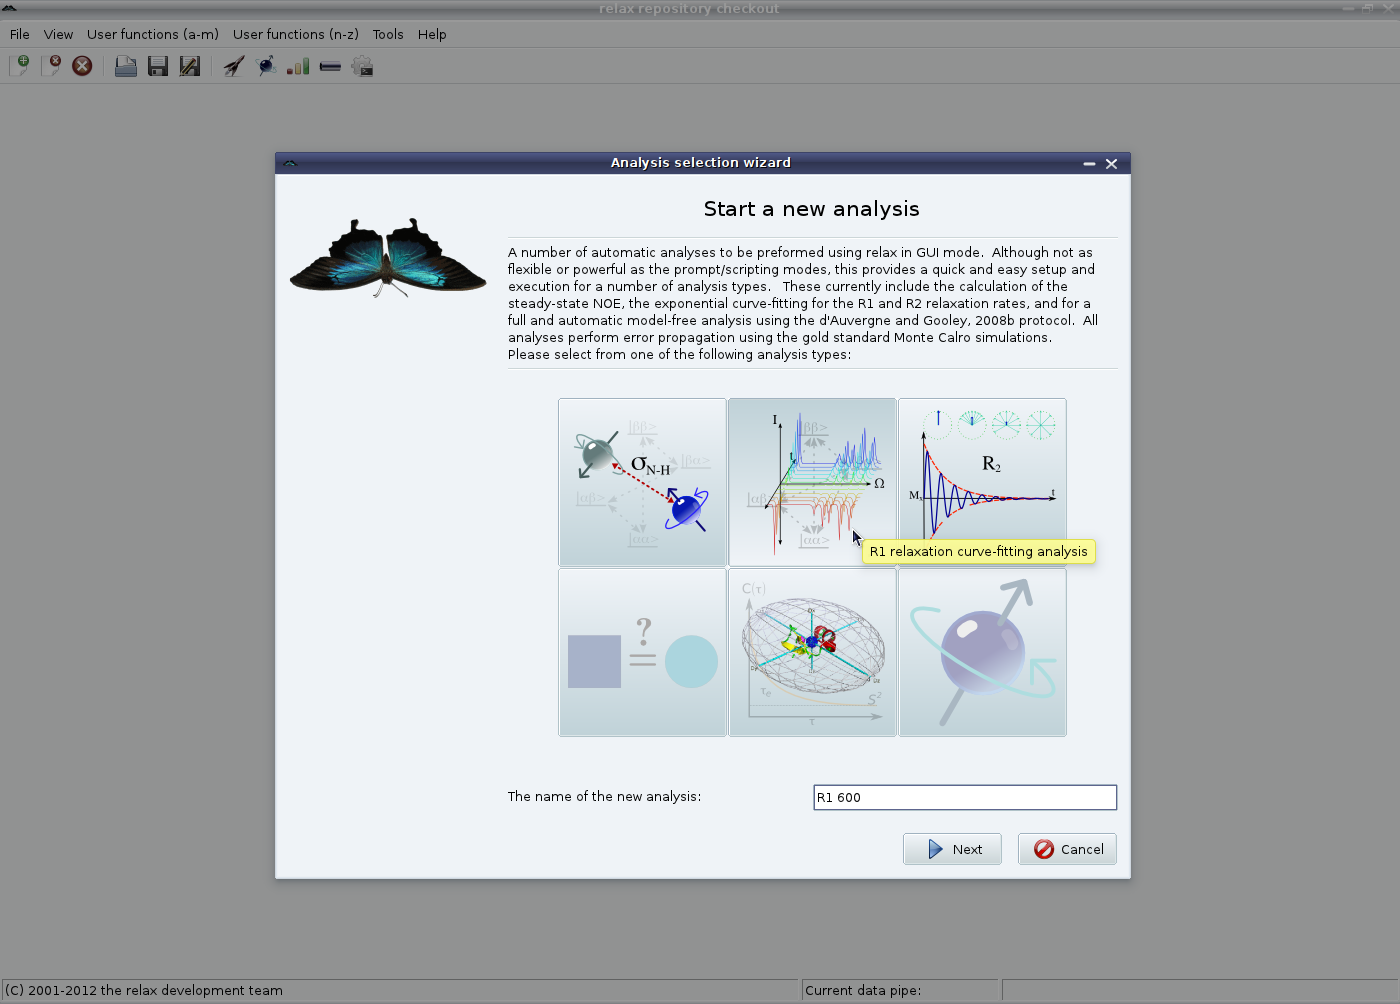
\includegraphics[width=0.8\textwidth, bb=14 14 1415 1019]{graphics/screenshots/r1_analysis/analysis_wizard1}}
\end{minipage}

Then click on the \guibutton{Next} button.  On the second page click on \guibutton{Start} to commence the analysis -- this second part of the wizard does not need to be changed.  For the $\Rone$ and $\Rtwo$ analyses in the GUI, a data pipe bundle containing only a single data pipe for that analysis will be created.  This data pipe bundle can be safely ignored.

\begin{minipage}[h]{\linewidth}
\centerline{\includegraphics[width=0.8\textwidth, bb=14 14 1415 1019]{graphics/screenshots/r1_analysis/analysis_wizard2}}
\end{minipage}


% General setup.
%~~~~~~~~~~~~~~~

\subsection{Relax-fit GUI mode -- general setup}

You will now be presented with a blank analysis tab:

\begin{minipage}[h]{\linewidth}
\centerline{\includegraphics[width=0.8\textwidth, bb=14 14 1415 1019]{graphics/screenshots/r1_analysis/blank}}
\end{minipage}

Here there are two things unique to the GUI which need to be preformed:

\begin{description}
\item[NMR frequency label:]  First set the NMR frequency label.  This is only used for the name of the output file.  For example if you set the label to \guistring{1200}, the file \file{r1.1200.out} will be created at the end of the analysis.
\item[Results directory:]  All of the automatically created results and Grace files will be placed into this directory.  The \gui{Results directory} can now be changed.
\end{description}


% Spin systems.
%~~~~~~~~~~~~~~

\subsection{Relax-fit GUI mode -- setting up the spin systems}

As the relaxation data is at the level of the spins, the molecule, residue and spin data structures need to be set up.  In the $\Rone$ and $\Rtwo$ GUI analysis tabs, there is a special \gui{Spin systems} GUI element designed for this.  This will initially say \gui{0 spins loaded and selected}.  Click on the \guibutton{Spin editor} button to launch the spin viewer window.  The steps for setting up the spin containers using PDB files are described in section~\ref{sect: GUI - structural data} on page~\pageref{sect: GUI - structural data} or for sequence files in section~\ref{sect: GUI - sequence file} on page~\pageref{sect: GUI - sequence file}.


% Unresolved spins.
%~~~~~~~~~~~~~~~~~~

\subsection{Relax-fit GUI mode -- unresolved spins}

As in the prompt/script UI section~\ref{sect: Rx setup fin}, the spins can be deselected at this point using the same \file{unresolved} file.  This is described in detail in section~\ref{sect: GUI - deselect spins} on page~\pageref{sect: GUI - deselect spins}.



% Loading the data.
%~~~~~~~~~~~~~~~~~~

\subsection{Relax-fit GUI mode -- loading the data}

At this stage, the peak intensity data needs to be loaded.  In both the $\Rone$ and $\Rtwo$ analysis tabs is a \gui{Spectra list} GUI element.  Click on the \guibutton{Add} button to launch the peak intensity loading wizard:

\begin{minipage}[h]{\linewidth}
\centerline{\includegraphics[width=0.8\textwidth, bb=14 14 1415 1019]{graphics/screenshots/r1_analysis/peak_intensity_bb_peaks}}
\end{minipage}

In this example, a Sparky peak list containing the peak heights determined from the averaged chemical shift positions for all spectra will be loaded.  Set the spectrum ID string to a unique value.  Change the heteronucleus and proton names to those of the $^{15}$N backbone assignments in the peak lists, in this case \gui{N} and \gui{NH}.

To load the tryptophan indole $^{15}$N spins as well, first click on \guibutton{Apply} rather than \guibutton{Next}.  This will most likely cause a \prompt{RelaxWarning} message to appear for all peak list elements which do not match the atom names given:

\begin{minipage}[h]{\linewidth}
\centerline{\includegraphics[width=0.8\textwidth, bb=14 14 1415 1019]{graphics/screenshots/r1_analysis/peak_intensity_warnings}}
\end{minipage}

These messages must be carefully checked to be sure that the correct data has been loaded.  A \prompt{RelaxError} might be thrown if the peak list is corrupted or if the atom names have been incorrectly given.  In this case, check the message, fix the problem, and click on \guibutton{Apply} again.

For the the tryptophan indole $^{15}$N spins, change the heteronucleus and proton names to \gui{NE1} and \gui{HE1} respectively (or to whatever you have named these in your assignments).  Then click on \guibutton{Next}:

\begin{minipage}[h]{\linewidth}
\centerline{\includegraphics[width=0.8\textwidth, bb=14 14 1415 1019]{graphics/screenshots/r1_analysis/peak_intensity_trp_peaks}}
\end{minipage}

Again check the messages in the relax controller window which will appear.  You should now see the error type page:

\begin{minipage}[h]{\linewidth}
\centerline{\includegraphics[width=0.8\textwidth, bb=14 14 1415 1019]{graphics/screenshots/r1_analysis/peak_intensity_err_type}}
\end{minipage}

The description for this wizard page should be very carefully read -- it will tell you about all of the error analysis options available and how these are implemented in relax.  For the protein relaxation example, replicated spectra have been collected.  Therefore the option \gui{Replicated spectra} will be chosen.  The \gui{Baseplane RMSD} option is documented in the NOE chapter.  After clicking on \guibutton{Next} you will see:

\begin{minipage}[h]{\linewidth}
\centerline{\includegraphics[width=0.8\textwidth, bb=14 14 1415 1019]{graphics/screenshots/r1_analysis/peak_intensity_replicates1}}
\end{minipage}

For the first of the duplicate spectra, or any spectrum without a duplicate, you can click on the \guibutton{Skip} button.  If this is the second spectrum you have loaded from a duplicated set, select the two replicated spectra and then click on \guibutton{Next}:

\begin{minipage}[h]{\linewidth}
\centerline{\includegraphics[width=0.8\textwidth, bb=14 14 1415 1019]{graphics/screenshots/r1_analysis/peak_intensity_replicates2}}
\end{minipage}

Finally set the relaxation time period for this experiment in seconds:

\begin{minipage}[h]{\linewidth}
\centerline{\includegraphics[width=0.8\textwidth, bb=14 14 1415 1019]{graphics/screenshots/r1_analysis/peak_intensity_times}}
\end{minipage}

All delays and pulse lengths in the pulse sequence should be carefully checked to be sure that the time is exactly what you would expect -- the estimated time may not match the real time.  To set the time and close the wizard, click on the \guibutton{Finish} button.

This procedure should be repeated for every experiment you have collected (you could, as an alternative, load all at the same time using the \guibutton{Apply} button at each stage).  In the end you should see something such as:

\begin{minipage}[h]{\linewidth}
\centerline{\includegraphics[width=0.8\textwidth, bb=14 14 1415 1019]{graphics/screenshots/r1_analysis/analysis_tab_full}}
\end{minipage}


% Optimisation and error analysis.
%~~~~~~~~~~~~~~~~~~~~~~~~~~~~~~~~~

\subsection{Relax-fit GUI mode -- optimisation and error analysis}

Back in the main $\Rone$ analysis tab, the grid search increments and number of Monte Carlo simulations can be changed.  The default values of 21 grid search increments and 500 MC simulations are optimal -- lower values are not recommended.  To perform the optimisation and error analysis, click on the \guibutton{Execute relax} button.  The relax controller will open to show you the progress of the optimisation and simulations:

\begin{minipage}[h]{\linewidth}
\centerline{\includegraphics[width=0.8\textwidth, bb=14 14 1415 1019]{graphics/screenshots/r1_analysis/mc_sim}}
\end{minipage}

Once finished, the \gui{Results viewer} window will also appear:

\begin{minipage}[h]{\linewidth}
\centerline{\includegraphics[width=0.8\textwidth, bb=14 14 1415 1019]{graphics/screenshots/r1_analysis/fin}}
\end{minipage}

This window can be used to open the text files in the default text editor for your operating system or the 2D Grace plots in \prompt{xmgrace} if available on your system.



% Final checks.
%%%%%%%%%%%%%%%

\section{Final checks of the curve-fitting}

To be sure that the data has been properly collected and that no instrumentation or pulse sequence timing errors have occurred, it is essential to carefully check the \file{intensities.agr} and \file{intensities\_norm.agr} 2D Grace\index{software!Grace|textbf} files.  These are plots of the decay curves for each spin system analysed, and any non-exponential behaviour should be clearly visible (see Figure~\ref{fig: screenshot: xmgrace peak intensities}).  If Xmgrace or a compatible program is not available for your operating system, the Grace files contain text representations of the curves at the end which can opened, edited and visualised in any another 2D graphing software package.
 
% Xmgrace screenshot
\begin{figure}
\centerline{\includegraphics[width=\textwidth, bb=14 14 923 724]{graphics/screenshots/xmgrace_peak_intensities}}
\caption[Peak intensity 2D plot xmgrace screenshot]{Screenshot of the 2D peak intensity plots for the exponential relaxation curves in Xmgrace.}\label{fig: screenshot: xmgrace peak intensities}
\end{figure}

Note that errors resulting in systematic bias in the data -- for example if temperature control (single-scan interleaving or temperature compensation blocks) or per-experiment/per-spectrometer temperature calibration on MeOH or ethylene glycol have not been performed -- will not be detected by looking at the decay curves.  See section~\ref{sect: temperature control and calibration} or the \uf{relax\_data.temp\_calibration} user function documentation on page~\pageref{uf: relax_data.temp_calibration} and the \uf{relax\_data.temp\_control} user function documentation on page~\pageref{uf: relax_data.temp_control} for more details.

% Model-free analysis.
%%%%%%%%%%%%%%%%%%%%%%

\chapter{Model-free analysis}
\label{ch: model-free}
\index{model-free analysis|textbf}



% Theory.
%%%%%%%%%

\section{Theory}



% The chi-squared function.
\begin{latexonly}
    \subsection{The chi-squared function -- $\chi^2(\theta)$}
\end{latexonly}
\begin{htmlonly}
    \subsection{The chi-squared function -- $chi^2(theta)$}
\begin{htmlonly}

\index{chi-squared|textbf}

For the minimisation\index{minimisation} of the model-free models a chain of calculations, each based on a different theory, is required.  At the highest level the equation which is actually minimised is the chi-squared function
\begin{equation} \label{eq: chi-squared}
 \chi^2(\theta) = \sum_{i=1}^n \frac{(\Ri - \Ri(\theta))^2}{\sigma_i^2},
\end{equation}

\noindent where the index $i$ is the summation index ranging over all the experimentally collected relaxation data of all spins used in the analysis; $\Ri$ belongs to the relaxation data set R for an individual spin, a collection of spins, or the entire macromolecule and includes the $\Rone$, $\Rtwo$, and NOE data at all field strengths; $\Ri(\theta)$ is the back-calculated relaxation value belonging to the set R$(\theta)$; $\theta$ is the model parameter vector which when minimised is denoted by $\hat\theta$; and $\sigma_i$ is the experimental error.

The significance of the chi-squared equation~\eqref{eq: chi-squared} is that the function returns a single value which is then minimised by the optimisation algorithm to find the model-free parameter values of the given model.



% The transformed relaxation equations.
\begin{latexonly}
    \subsection{The transformed relaxation equations -- $\Ri(\theta)$}
\end{latexonly}
\begin{htmlonly}
    \subsection{The transformed relaxation equations -- R$_i(theta)$}
\end{htmlonly}

The chi-squared equation is itself dependent on the relaxation equations through the back-calculated relaxation data R$(\theta)$.  Letting the relaxation values of the set R$(\theta)$ be the $\Rone(\theta)$, $\Rtwo(\theta)$, and NOE$(\theta)$ an additional layer of abstraction can be used to simplify the calculation of the gradients and Hessians.  This involves decomposing the NOE equation into the cross relaxation rate constant $\crossrate(\theta)$ and the auto relaxation rate $\Rone(\theta)$.  Taking equation~\eqref{eq: NOE} below the transformed relaxation equations are
\begin{subequations}
\begin{align}
    \Rone(\theta) &= \Rone'(\theta), \\
    \Rtwo(\theta) &= \Rtwo'(\theta), \\
    \mathrm{NOE}(\theta)  &= 1 + \frac{\gH}{\gX} \frac{\crossrate(\theta)}{\Rone(\theta)}.
\end{align}
\end{subequations}

\noindent whereas the relaxation equations are the $\Rone(\theta)$, $\Rtwo(\theta)$, $\crossrate(\theta)$.



% The relaxation equations.
\begin{latexonly}
    \subsection{The relaxation equations -- $\Ri'(\theta)$}
\end{latexonly}
\begin{htmlonly}
    \subsection{The relaxation equations -- R$_i$ $prime(theta)$}
\end{htmlonly}

The relaxation values of the set R$'(\theta)$ include the spin-lattice\index{relaxation rate!spin-lattice}, spin-spin\index{relaxation rate!spin-spin}, and cross-relaxation rates\index{relaxation rate!cross rate} at all field strengths.  These rates are respectively \citep{Abragam61}
\begin{subequations}
\begin{align}
    \Rone(\theta) &= d \Big( J(\omega_H - \omega_X) + 3J(\omega_X) + 6J(\omega_H + \omega_X) \Big) + cJ(\omega_X),     \label{eq: R1} \\
    \Rtwo(\theta) &= \frac{d}{2} \Big( 4J(0) + J(\omega_H - \omega_X) + 3J(\omega_X) + 6J(\omega_H)                    \nonumber \\
        & \quad + 6J(\omega_H + \omega_X) \Big) + \frac{c}{6} \Big( 4J(0) + 3J(\omega_X) \Big) + R_{ex},              \label{eq: R2} \\  
    \crossrate(\theta) &= d \Big( 6J(\omega_H + \omega_X) - J(\omega_H - \omega_X) \Big),                              \label{eq: sigma_NOE}
\end{align}
\end{subequations}

\noindent where $J(\omega)$ is the power spectral density function and $R_{ex}$ is the relaxation due to chemical exchange.  The dipolar and CSA constants are defined in SI units as
\begin{gather}
 d = \frac{1}{4} \left(\frac{\mu_0}{4\pi}\right)^2 \frac{(\gH \gX \hbar)^2}{\langle r^6 \rangle}, \label{eq: dipolar constant} \\
 c = \frac{(\omega_H \Delta\sigma)^2}{3}, \label{eq: CSA constant}
\end{gather}

\noindent where $\mu_0$ is the permeability of free space, $\gH$ and $\gX$ are the gyromagnetic ratios of the $H$ and $X$ spins respectively, $\hbar$ is Plank's constant divided by $2\pi$, $r$ is the bond length, and $\Delta\sigma$ is the chemical shift anisotropy measured in ppm.  The cross-relaxation rate $\crossrate$\index{relaxation rate!cross-relaxation|textbf} is related to the steady state NOE by the equation
\begin{equation} \label{eq: NOE}
 \mathrm{NOE}(\theta) = 1 + \frac{\gH}{\gX} \frac{\crossrate(\theta)}{\Rone(\theta)}.
\end{equation}



% The spectral density functions.
\begin{latexonly}
    \subsection{The spectral density functions -- $J(\omega)$}
\end{latexonly}
\begin{htmlonly}
    \subsection{The spectral density functions -- $J(omega)$}
\end{htmlonly}

The relaxation equations are themselves dependent on the calculation of the spectral density values $J(\omega)$.  Within model-free analysis these are modelled by the original model-free formula \citep{LipariSzabo82a, LipariSzabo82b}
\begin{equation} \label{eq: J(w) model-free generic}
    J(\omega) = \frac{2}{5} \sum_{i=-k}^k c_i \cdot \tau_i \Bigg(
        \frac{S^2}{1 + (\omega \tau_i)^2}
        + \frac{(1 - S^2)(\tau_e + \tau_i)\tau_e}{(\tau_e + \tau_i)^2 + (\omega \tau_e \tau_i)^2}
    \Bigg),
\end{equation}

\noindent where $S^2$ is the square of the Lipari and Szabo generalised order parameter and $\tau_e$ is the effective correlation time.  The order parameter reflects the amplitude of the motion and the correlation time in an indication of the time scale of that motion.  The theory was extended by \citet{Clore90a} by the modelling of two independent internal motions using the equation
\begin{multline} \label{eq: J(w) model-free ext generic}
    J(\omega) = \frac{2}{5} \sum_{i=-k}^k c_i \cdot \tau_i \Bigg(
        \frac{S^2}{1 + (\omega \tau_i)^2}
        + \frac{(1 - S^2_f)(\tau_f + \tau_i)\tau_f}{(\tau_f + \tau_i)^2 + (\omega \tau_f \tau_i)^2}       \\
        + \frac{(S^2_f - S^2)(\tau_s + \tau_i)\tau_s}{(\tau_s + \tau_i)^2 + (\omega \tau_s \tau_i)^2}
    \Bigg).
\end{multline}

\noindent where $S^2_f$ and $\tau_f$ are the amplitude and timescale of the faster of the two motions whereas $S^2_s$ and $\tau_s$ are those of the slower motion.  $S^2_f$ and $S^2_s$ are related by the formula $S^2 = S^2_f \cdot S^2_s$.



% Brownian rotational diffusion.
\subsection{Brownian rotational diffusion}

\index{diffusion!Brownian|textbf}
In equations~\eqref{eq: J(w) model-free generic} and~\eqref{eq: J(w) model-free ext generic} the generic Brownian diffusion NMR correlation function presented in \citet{dAuvergne06} has been used.  This function is
\begin{equation} \label{eq: C(tau) generic}
    C(\tau) = \frac{1}{5} \sum_{i=-k}^k c_i \cdot e^{-\tau/\tau_i},
\end{equation}

\noindent where the summation index $i$ ranges over the number of exponential terms within the correlation function.  This equation is generic in that it can describe the diffusion\index{diffusion} of an ellipsoid, a spheroid, or a sphere.



% Diffusion as an ellipsoid.
\subsubsection{Diffusion as an ellipsoid}
\index{diffusion!ellipsoid (asymmetric)|textbf}

For the ellipsoid defined by the parameter set \{$\Diff_{iso}$, $\Diff_a$, $\Diff_r$, $\alpha$, $\beta$, $\gamma$\} the variable $k$ is equal to two and therefore the index $i \in \{-2, -1, 0, 1, 2\}$.  The geometric parameters \{$\Diff_{iso}$, $\Diff_a$, $\Diff_r$\} are defined as
\begin{subequations}
\begin{align}
    & \Diff_{iso} = \tfrac{1}{3} (\Diff_x + \Diff_y + \Diff_z ),   \label{eq: Diso ellipsoid def} \\
    & \Diff_a = \Diff_z - \tfrac{1}{2}(\Diff_x + \Diff_y),         \label{eq: Da ellipsoid def} \\
    & \Diff_r = \frac{\Diff_y - \Diff_x}{2\Diff_a},                \label{eq: Dr ellipsoid def}
\end{align}
\end{subequations}

\noindent and are constrained by
\begin{subequations}
\begin{align}
    0 & < \Diff_{iso} < \infty,                                                    \label{eq: Diso lim} \\
    0 & \le \Diff_a < \frac{\Diff_{iso}}{\tfrac{1}{3} + \Diff_r} \le 3\Diff_{iso}, \label{eq: Da lim} \\
    0 & \le \Diff_r \le 1.                                                         \label{eq: Dr lim}
\end{align}
\end{subequations}

\noindent The orientational parameters \{$\alpha$, $\beta$, $\gamma$\} are the Euler angles using the z-y-z rotation notation.


The five weights $c_i$ are defined as
\begin{subequations}
\begin{align}
    c_{-2} &= \tfrac{1}{4}(d - e),     \label{eq: ellipsoid c-2} \\
    c_{-1} &= 3\delta_y^2\delta_z^2,   \label{eq: ellipsoid c-1} \\
    c_{0}  &= 3\delta_x^2\delta_z^2,   \label{eq: ellipsoid c0} \\
    c_{1}  &= 3\delta_x^2\delta_y^2,   \label{eq: ellipsoid c1} \\
    c_{2}  &= \tfrac{1}{4}(d + e),     \label{eq: ellipsoid c2}
\end{align}
\end{subequations}

\noindent where
\begin{align}
    d &= 3 \left( \delta_x^4 + \delta_y^4 + \delta_z^4 \right) - 1, \label{eq: ellipsoid d} \\
    e &= \frac{1}{\mathfrak{R}} \bigg[ (1 + 3\Diff_r) \left(\delta_x^4 + 2\delta_y^2\delta_z^2\right)
        + (1 - 3\Diff_r) \left(\delta_y^4 + 2\delta_x^2\delta_z^2\right) - 2 \left(\delta_z^4 + 2\delta_x^2\delta_y^2\right) \bigg], \label{eq: ellipsoid e}
\end{align}

\noindent and where
\begin{equation}
    \mathfrak{R} = \sqrt{1 + 3\Diff_r^2}.
\end{equation}


The five correlation times $\tau_i$ are
\begin{subequations}
\begin{align}
    1/\tau_{-2} &= 6 \Diff_{iso} - 2\Diff_a\mathfrak{R},   \label{eq: ellipsoid tau-2} \\
    1/\tau_{-1} &= 6 \Diff_{iso} - \Diff_a (1 + 3\Diff_r), \label{eq: ellipsoid tau-1} \\
    1/\tau_{0}  &= 6 \Diff_{iso} - \Diff_a (1 - 3\Diff_r), \label{eq: ellipsoid tau0} \\
    1/\tau_{1}  &= 6 \Diff_{iso} + 2\Diff_a,               \label{eq: ellipsoid tau1} \\
    1/\tau_{2}  &= 6 \Diff_{iso} + 2\Diff_a\mathfrak{R}.   \label{eq: ellipsoid tau2}
\end{align}
\end{subequations}



% Diffusion as a spheroid.
\subsubsection{Diffusion as a spheroid}
\index{diffusion!spheroid (axially symmetric)|textbf}

The variable $k$ is equal to one in the case of the spheroid\index{diffusion!spheroid (axially symmetric)|textbf} defined by the parameter set \{$\Diff_{iso}$, $\Diff_a$, $\theta$, $\phi$\}, hence $i \in \{-1, 0, 1\}$.  The geometric parameters \{$\Diff_{iso}$, $\Diff_a$\} are defined as
\begin{subequations}
\begin{align}
    & \Diff_{iso} = \tfrac{1}{3} (\Diff_\Par + 2\Diff_\Per),   \label{eq: Diso spheroid def} \\
    & \Diff_a = \Diff_\Par - \Diff_\Per.                       \label{eq: Da spheroid def}
\end{align}
\end{subequations}

\noindent and are constrained by
\begin{subequations}
\begin{gather}
    0 < \Diff_{iso} < \infty, \\
    -\tfrac{3}{2} \Diff_{iso} < \Diff_a < 3\Diff_{iso}.
\end{gather}
\end{subequations}

\noindent The orientational parameters \{$\theta$, $\phi$\} are the spherical angles defining the orientation of the major axis of the diffusion frame within the lab frame.


The three weights $c_i$ are
\begin{subequations}
\begin{align}
    c_{-1} &= \tfrac{1}{4}(3\delta_z^2 - 1)^2, \label{eq: spheroid c-1} \\
    c_{0}  &= 3\delta_z^2(1 - \delta_z^2),     \label{eq: spheroid c0} \\
    c_{1}  &= \tfrac{3}{4}(\delta_z^2 - 1)^2.  \label{eq: spheroid c1}
\end{align}
\end{subequations}

The five correlation times $\tau_i$ are
\begin{subequations}
\begin{align}
    1/\tau_{-1} &= 6\Diff_{iso} - 2\Diff_a,    \label{eq: spheroid tau-1} \\
    1/\tau_{0}  &= 6\Diff_{iso} - \Diff_a,     \label{eq: spheroid tau0} \\
    1/\tau_{1}  &= 6\Diff_{iso} + 2\Diff_a.    \label{eq: spheroid tau1}
\end{align}
\end{subequations}



% Diffusion as a sphere.
\subsubsection{Diffusion as a sphere}
\index{diffusion!sphere (isotropic)|textbf}

In the situation of a molecule diffusing as a sphere\index{diffusion!sphere (isotropic)|textbf} either described by the single parameter $\tau_m$ or $\Diff_{iso}$, the variable $k$ is equal to zero.  Therefore $i \in \{0\}$.  The single weight $c_0$ is equal to one and the single correlation time $\tau_0$ is equivalent to the global tumbling time $\tau_m$ given by
\begin{equation} \label{eq: sphere tau0}
    1/\tau_m = 6\Diff_{iso}.
\end{equation}

\noindent This is diffusion equation presented in \citet{Bloembergen48}.


% The model-free models.
%~~~~~~~~~~~~~~~~~~~~~~~

\subsection{The model-free models}

Extending the list of models given in \citet{Mandel95, Fushman97, Orekhov99b, Korzhnev01, Zhuravleva04}, the models built into relax include
\begin{subequations}
\renewcommand{\theequation}{\theparentequation .\arabic{equation}}
\addtocounter{equation}{-1}
\begin{align}
 m0 &= \{\},                                   \label{model: m0} \\
 m1 &= \{S^2\},                                \label{model: m1} \\
 m2 &= \{S^2, \tau_e\},                        \label{model: m2} \\
 m3 &= \{S^2, R_{ex}\},                        \label{model: m3} \\
 m4 &= \{S^2, \tau_e, R_{ex}\},                \label{model: m4} \\
 m5 &= \{S^2, S^2_f, \tau_s\},                 \label{model: m5} \\
 m6 &= \{S^2, \tau_f, S^2_f, \tau_s\},         \label{model: m6} \\
 m7 &= \{S^2, S^2_f, \tau_s, R_{ex}\},         \label{model: m7} \\
 m8 &= \{S^2, \tau_f, S^2_f, \tau_s, R_{ex}\}, \label{model: m8} \\
 m9 &= \{R_{ex}\}.                             \label{model: m9}
\end{align}
\end{subequations}

\noindent The parameter $R_{ex}$ is scaled quadratically with field strength in these models as it is assumed to be fast.  In the set theory notation, the model-free model for the spin system $i$ is represented by the symbol $\Mfset_i$.  Through the addition of the local $\tau_m$ to each of these models, only the component of Brownian rotational diffusion experienced by the spin system is probed.  These models, represented in set notation by the symbol $\Localset_i$, are
\begin{subequations}
\renewcommand{\theequation}{\theparentequation .\arabic{equation}}
\addtocounter{equation}{-1}
\begin{align}
 tm0 &= \{\tau_m\},                                     \label{model: tm0} \\
 tm1 &= \{\tau_m, S^2\},                                \label{model: tm1} \\
 tm2 &= \{\tau_m, S^2, \tau_e\},                        \label{model: tm2} \\
 tm3 &= \{\tau_m, S^2, R_{ex}\},                        \label{model: tm3} \\
 tm4 &= \{\tau_m, S^2, \tau_e, R_{ex}\},                \label{model: tm4} \\
 tm5 &= \{\tau_m, S^2, S^2_f, \tau_s\},                 \label{model: tm5} \\
 tm6 &= \{\tau_m, S^2, \tau_f, S^2_f, \tau_s\},         \label{model: tm6} \\
 tm7 &= \{\tau_m, S^2, S^2_f, \tau_s, R_{ex}\},         \label{model: tm7} \\
 tm8 &= \{\tau_m, S^2, \tau_f, S^2_f, \tau_s, R_{ex}\}, \label{model: tm8} \\
 tm9 &= \{\tau_m, R_{ex}\}.                             \label{model: tm9}
\end{align}
\end{subequations}




% Model-free optimisation theory.
%~~~~~~~~~~~~~~~~~~~~~~~~~~~~~~~~

\subsection{Model-free optimisation theory}


% The model-free space.
\subsubsection{The model-free space}

The optimisation of the parameters of an arbitrary model is dependent on a function $f$ which takes the current parameter values $\theta \in \mathbb{R}^n$ and returns a single real value $f(\theta) \in \mathbb{R}$ corresponding to position $\theta$ in the $n$-dimensional space.  For it is that single value which is minimised as
\begin{equation}
 \hat\theta = \arg \min_\theta f(\theta),
\end{equation}

\noindent where $\hat\theta$ is the parameter vector which is equal to the argument which minimises the function $f(\theta)$.  In model-free analysis $f(\theta)$ is the chi-squared\index{chi-squared|textbf} equation
\begin{equation} \label{eq: chi2}
 \chi^2(\theta) = \sum_{i=1}^n \frac{(\Ri - \Ri(\theta))^2}{\sigma_i^2},
\end{equation}

\noindent where $i$ is the summation index, $\Ri$ is the experimental relaxation data which belongs to the data set R and includes the $\Rone$, $\Rtwo$, and NOE values at all field strengths, $\Ri(\theta)$ is the back calculated relaxation data belonging to the set R$(\theta)$, and $\sigma_i$ is the experimental error.  For the optimisation of the model-free parameters while the diffusion tensor is held fixed, the summation index ranges over the relaxation data of an individual spin.  If the diffusion parameters are optimised simultaneously with the model-free parameters the summation index ranges over all relaxation data of all selected spins of the macromolecule.

Given the current parameter values the model-free function provided to the algorithm will calculate the value of the model-free spectral density function $J(\omega)$ at the five frequencies which induce NMR relaxation by using Equations~\eqref{eq: J(w) model-free generic} and \eqref{eq: J(w) model-free ext generic}.  The theoretical $\Rone$, $\Rtwo$, and NOE values are then back-calculated using Equations~\eqref{eq: R1}, \eqref{eq: R2}, \eqref{eq: sigma_NOE}, and \eqref{eq: NOE}.  Finally, the chi-squared\index{chi-squared} value is calculated using Equation~\eqref{eq: chi2}.


% Topology of the space.
\subsubsection{Topology of the space}

The problem of finding the minimum is complicated by the fact that optimisation algorithms are blind to the curvature of the complete space.  Instead they rely on topological information about the current and, sometimes, the previous parameter positions in the space.  The techniques use this information to walk iteratively downhill to the minimum.  Very few optimisation algorithms rely solely on the function value, conceptually the height of the space, at the current position.  Most techniques also utilise the gradient at the current position.  Although symbolically complex in the case of model-free analysis, the gradient can simply be calculated as the vector of first partial derivatives of the chi-squared\index{chi-squared} equation with respect to each model-free parameter.  The gradient is supplied as a second function to the algorithm which is then utilised in diverse ways by different optimisation techniques.  The function value together with the gradient can be combined to construct a linear or planar description of the space at the current parameter position by first-order Taylor series approximation
\begin{equation} \label{eq: linear model}
 f(\theta_k + x) \approx f_k  +  x^T \nabla f_k,
\end{equation}

\noindent where $f_k$ is the function value at the current parameter position $\theta_k$, $\nabla f_k$ is the gradient at the same position, and $x$ is an arbitrary vector.  By accumulating information from previous parameter positions a more comprehensive geometric description of the curvature of the space can be exploited by the algorithm for more efficient optimisation.

The best and most comprehensive description of the space is given by the quadratic approximation of the topology which is generated from the combination of the function value, the gradient, and the Hessian.  From the second-order Taylor series expansion the quadratic model of the space is
\begin{equation} \label{eq: quadratic model}
 f(\theta_k + x) \approx f_k  +  x^T \nabla f_k  +  \tfrac{1}{2} x^T \nabla^2 f_k x,
\end{equation}

\noindent where $\nabla^2 f_k$ is the Hessian, which is the symmetric matrix of second partial derivatives of the function, at the position $\theta_k$.  As the Hessian is computationally expensive a number of optimisation algorithms try to approximate it.

To produce the gradient and Hessian required for model-free optimisation a large chain of first and second partial derivatives needs to be calculated.  Firstly the partial derivatives of the spectral density functions \eqref{eq: J(w) model-free generic} and \eqref{eq: J(w) model-free ext generic} are necessary.  Then the partial derivatives of the relaxation equations~\eqref{eq: R1} to~\eqref{eq: sigma_NOE} followed by the NOE equation~\eqref{eq: NOE} are needed.  Finally the partial derivative of the chi-squared\index{chi-squared} formula~\eqref{eq: chi2} is required.  These first and second partial derivatives, as well as those of the components of the Brownian diffusion correlation function for non-isotropic tumbling, are presented in Chapter~\ref{ch: values, gradients, and Hessians}.



% Optimisation algorithms.
\subsubsection{Optimisation algorithms}

Prior to minimisation, all optimisation algorithms investigated require a starting position within the model-free space.  This initial parameter vector is found by employing a coarse grid search -- chi-squared\index{chi-squared} values at regular positions spanning the space are calculated and the grid point with the lowest value becomes the starting position.  The grid search itself is an optimisation technique.  As it is computationally expensive the number of grid points needs to be kept to a minimum.  Hence the initial parameter values are a rough and imprecise approximation of the local minimum.  Due to the complexity of the curvature of the model-free space, the grid point with the lowest chi-squared\index{chi-squared} value may in fact be on the opposite side of the space to the local minimum.

Once the starting position has been determined by the grid search the optimisation algorithm can be executed.  The number of algorithms developed within the mathematical field of optimisation is considerable.  They can nevertheless be grouped into one of a small number of major categories based on the fundamental principles of the technique.  These include the line search methods, the trust region methods, and the conjugate gradient methods.  For more details on the algorithms described below see \citet{NocedalWright99}.



% Line search methods.
\subsubsection{Line search methods}

The defining characteristic of a line search algorithm is to choose a search direction $p_k$ and then to find the minimum along that vector starting from $\theta_k$ \citep{NocedalWright99}.  The distance travelled along $p_k$ is the step length $\alpha_k$ and the parameter values for the next iteration are
\begin{equation}
 \theta_{k+1} = \theta_k + \alpha_k p_k.
\end{equation}

\noindent  The line search algorithm determines the search direction $p_k$ whereas the value of $\alpha_k$ is found using an auxiliary step-length selection algorithm.

One of the simplest line search methods is the steepest descent\index{minimisation algorithm!steepest descent|textbf} algorithm.  The search direction is simply the negative gradient, $p_k = -\nabla f_k$, and hence the direction of maximal descent is always followed.  This method is inefficient -- the linear rate of convergence requires many iterations of the algorithm to reach the minimum and it is susceptible to being trapped on saddle points within the space.

The coordinate descent\index{minimisation algorithm!coordinate descent|textbf} algorithms are a simplistic group of line search methods whereby the search directions alternate between vectors parallel to the parameter axes.  For the back-and-forth coordinate descent the search directions cycle in one direction and then back again.  For example for a three parameter model the search directions cycle $\theta_1, \theta_2, \theta_3, \theta_2, \theta_1, \theta_2, \hdots$, which means that each parameter of the model is optimised one by one.  The method becomes less efficient when approaching the minimum as the step length $\alpha_k$ continually decreases (ibid.).

The quasi-Newton methods begin with an initial guess of the Hessian and update it at each iteration using the function value and gradient.  Therefore the benefits of using the quadratic model of \eqref{eq: quadratic model} are obtained without calculating the computationally expensive Hessian.  The Hessian approximation $B_k$ is updated using various formulae, the most common being the BFGS\index{minimisation algorithm!BFGS|textbf} formula \citep{Broyden70,Fletcher70,Goldfarb70,Shanno70}.  The search direction is given by the equation $p_k = -B_k^{-1} \nabla f_k$.  The quasi-Newton algorithms can attain a superlinear rate of convergence, being superior to the steepest descent or coordinate descent methods.

The most powerful line search method when close to the minimum is the Newton\index{minimisation algorithm!Newton|textbf} search direction
\begin{equation} \label{eq: Newton dir}
 p_k = - \nabla^2 f_k^{-1} \nabla f_k.
\end{equation}

\noindent This direction is obtained from the derivative of \eqref{eq: quadratic model} which is assumed to be zero at the minimum of the quadratic model.  The vector $p_k$ points from the current position to the exact minimum of the quadratic model of the space.  The rate of convergence is quadratic, being superior to both linear and superlinear convergence.  The technique is computationally expensive due to the calculation of the Hessian.  It is also susceptible to failure when optimisation commences from distant positions in the space as the Hessian may not be positive definite and hence not convex, a condition required for the search direction both to point downhill and to be reasonably oriented.  In these cases the quadratic model is a poor description of the space.

A practical Newton algorithm which is robust for distant starting points is the Newton conjugate gradient method (Newton-CG\index{minimisation algorithm!Newton-CG|textbf}).  This line search method, which is also called the truncated Newton algorithm, finds an approximate solution to Equation~\eqref{eq: Newton dir} by using a conjugate gradient (CG) sub-algorithm.  Retaining the performance of the pure Newton algorithm, the CG sub-algorithm guarantees that the search direction is always downhill as the method terminates when negative curvature is encountered.  This algorithm is similar to the Newton-Raphson-CG algorithm implemented within Dasha\index{software!Dasha}.  Newton optimisation is sometimes also known as the Newton-Raphson algorithm and, as documented in the source code, the Newton algorithm in Dasha is coupled to a conjugate gradient algorithm.  The auxiliary ste\mbox{p-l}ength selection algorithm in Dasha\index{software!Dasha} is undocumented and may not be employed.

Once the search direction has been determined by the above algorithms the minimum along that direction needs to be determined.  Not to be confused with the methodology for determining the search direction $p_k$, the line search itself is performed by an auxiliary step-length selection algorithm to find the value $\alpha_k$.  A number of step-length selection methods can be used to find a minimum along the line $\theta_k + \alpha_k p_k$, although only two will be investigated.  The first is the backtracking line search of \citet{NocedalWright99}.  This method is inexact -- it takes a starting step length $\alpha_k$ and decreases the value until a sufficient decrease in the function is found.  The second is the line search method of \citet{MoreThuente94}.  Designed to be robust, the MT algorithm finds the exact minimum along the search direction and guarantees sufficient decrease.



% Trust region methods.
\subsubsection{Trust region methods}

In the trust region class of algorithms the curvature of the space is modelled quadratically by \eqref{eq: quadratic model}.  This model is assumed to be reliable only within a region of trust defined by the inequality $\lVert p \rVert \leqslant \Delta_k$ where $p$ is the step taken by the algorithm and $\Delta_k$ is the radius of the $n$-dimensional sphere of trust \citep{NocedalWright99}.  The solution sought for each iteration of the algorithm is
\begin{equation} \label{eq: trust region}
 \min_{p \in \mathbb{R}^n} m_k(p) = f_k  +  p^{T} \nabla f_k  +  \tfrac{1}{2} p^{T} B_k p,  \qquad \textrm{s.t. } \lVert p \rVert \leqslant \Delta_k,
\end{equation}

\noindent where $m_k(p)$ is the quadratic model, $B_k$ is a positive definite matrix which can be the true Hessian as in the Newton model or an approximation such as the BFGS\index{minimisation algorithm!BFGS} matrix, and $\lVert p \rVert$ is the Euclidean norm of $p$.  The trust region radius $\Delta_k$ is modified dynamically during optimisation -- if the quadratic model is found to be a poor representation of the space the radius is decreased whereas if the quadratic model is found to be reasonable the radius is increased to allow larger, more efficient steps to be taken.

The Cauchy point\index{minimisation algorithm!Cauchy point|textbf} algorithm is similar in concept to the steepest descent\index{minimisation algorithm!steepest descent} line search algorithm.  The Cauchy point is the point lying on the gradient which minimises the quadratic model subject to the step being within the trust region.  By iteratively finding the Cauchy point the local minimum can be found.  The convergence of the technique is inefficient, being similar to that of the steepest descent algorithm.

In changing the trust region radius the exact solutions to \eqref{eq: trust region} map out a curved trajectory which starts parallel to the gradient for small radii.  The end of the trajectory, which occurs for radii greater than the step length, is the bottom of the quadratic model.  The dogleg\index{minimisation algorithm!dogleg|textbf} algorithm attempts to follow a similar path by first finding the minimum along the gradient and then finding the minimum along a trajectory from the current point to the bottom of the quadratic model.  The minimum along the second path is either the trust region boundary or the quadratic solution.  The matrix $B_k$ of \eqref{eq: trust region} can be the BFGS matrix, the unmodified Hessian, or a Hessian modified to be positive definite.

Another trust region algorithm is Steihaug's\index{minimisation algorithm!CG-Steihaug|textbf} modified conjugate gradient approach \citep{Steihaug83}.  For each step $k$ an iterative technique is used which is almost identical to the standard conjugate gradient procedure except for two additional termination conditions.  The first is if the next step is outside the trust region, the second is if a direction of zero or negative curvature is encountered.

An almost exact solution to \eqref{eq: trust region} can be found using an algorithm described in \citet{NocedalWright99}.  This exact trust region\index{minimisation algorithm!exact trust region|textbf} algorithm aims to precisely find the minimum of the quadratic model $m_k$ of the space within the trust region $\Delta_k$.  Any matrix $B_k$ can be used to construct the quadratic model.  However, the technique is computationally expensive.



% Conjugate gradient methods.
\subsubsection{Conjugate gradient methods}

The conjugate gradient algorithm (CG) was originally designed as a mathematical technique for solving a large system of linear equations \citet{HestenesStiefel52}, but was later adapted to solving nonlinear optimisation problems \citep{FletcherReeves64}.  The technique loops over a set of directions $p_0$, $p_1$, $\hdots$, $p_n$ which are all conjugate to the Hessian \citep{NocedalWright99}, a property defined as
\begin{equation}
 p_i^T \nabla^2 f_k p_j = 0,  \qquad \textrm{for all } i \ne j.
\end{equation}

\noindent By performing line searches over all directions $p_j$ the solution to the quadratic model \eqref{eq: quadratic model} of the position $\theta_k$ will be found in $n$ or less iterations of the CG algorithm where $n$ is the total number of parameters in the model.  The technique performs well on large problems with many parameters as no matrices are calculated or stored.  The algorithms perform better than the steepest descent method and preconditioning of the system is used to improve optimisation.  A number of preconditioned techniques will be investigated including the Fletcher-Reeves\index{minimisation algorithm!Fletcher-Reeves|textbf} algorithm which was the original conjugate gradient optimisation technique \citep{FletcherReeves64}, the Polak-Ribi\`ere\index{minimisation algorithm!Polak-Ribi\`ere|textbf} method \citep{PolakRibiere69}, a modified Polak-Ribi\`ere method called the Polak-Ribi\`ere +\index{minimisation algorithm!Polak-Ribi\`ere~+|textbf} method \citep{NocedalWright99}, and the Hestenes-Stiefel\index{minimisation algorithm!Hestenes-Stiefel|textbf} algorithm which originates from a formula in \citet{HestenesStiefel52}.  As a line search is performed to find the minimum along each conjugate direction both the backtracking and Mor\'e and Thuente auxiliary step-length selection algorithms will be tested with the CG algorithms.



% Hessian modifications.
\subsubsection{Hessian modifications}

The Newton search direction, used in both the line search and trust region methods, is dependent on the Hessian being positive definite for the quadratic model to be convex so that the search direction points sufficiently downhill.  This is not always the case as saddle points and other non-quadratic features of the space can be problematic.  Two classes of algorithms can be used to handle this situation.  The first involves using the conjugate gradient method as a sub-algorithm for solving the Newton problem for the step $k$.  The Newton-CG\index{minimisation algorithm!Newton-CG} line search algorithm described above is one such example.  The second class involves modifying the Hessian prior to, or at the same time as, finding the Newton step to guarantee that the replacement matrix $B_k$ is positive definite.  The convexity of $B_k$ is ensured by its eigenvalues all being positive.  The performance of two of these methods within the model-free space will be investigated.

The first modification uses the Cholesky factorisation of the matrix $B_k$, initialised to the true Hessian, to test for convexity (Algorithm 6.3 of \citet{NocedalWright99}).  If factorisation fails the matrix is not positive definite and a constant $\tau_k$ times the identity matrix $I$ is then added to $B_k$.  The constant originates from the Robbins norm of the Hessian $\lVert \nabla^2 f_k \rVert_F$ and is steadily increased until the factorisation is successful.  The resultant Cholesky lower triangular matrix $L$ can then be used to find the approximate Newton direction.  If $\tau_k$ is too large the convergence of this technique can approach that of the steepest descent\index{minimisation algorithm!steepest descent} algorithm.

The second method is the Gill, Murray, and Wright (GMW) algorithm \citep{GMW81} which modifies the Hessian during the execution of the Cholesky factorisation $\nabla^2 f_k = LIL^T$, where $L$ is a lower triangular matrix and $D$ is a diagonal matrix.  Only a single factorisation is required.  As rows and columns are interchanged during the algorithm the technique may be slow for large problems such as the optimisation of the model-free parameters of all spins together with the diffusion tensor parameters.  The rate of convergence of the technique is quadratic.



% Other methods.
\subsubsection{Other methods}

Two other optimisation algorithms which cannot be classified within line search, trust region, or conjugate gradient categories will also be investigated.  The first is the well known simplex\index{minimisation algorithm!simplex|textbf} optimisation algorithm.  The technique is often used as the only the function value is employed and hence the derivation of the gradient and Hessian can be avoided.  The simplex is created as an $n$-dimensional geometric object with $n+1$ vertices.  The first vertex is the starting position.  Each of the other $n$ vertices are created by shifting the starting position by a small amount parallel to one of unit vectors defining the coordinate system of the space.  Four simple rules are used to move the simplex through the space: reflection, extension, contraction, and a shrinkage of the entire simplex.  The result of these movements is that the simplex moves in an ameoboid-like fashion downhill, shrinking to pass through tight gaps and expanding to quickly move through non-convoluted space, eventually finding the minimum.

Key to these four movements is the pivot point, the centre of the face created by the $n$ vertices with the lowest function values.  The first movement is a reflection -- the vertex with the greatest function value is reflected through the pivot point on the opposite face of the simplex.  If the function value at this new position is less than all others the simplex is allowed to extend -- the point is moved along the line to twice the distance between the current position and the pivot point.  Otherwise if the function value is greater than the second highest value but less than the highest value, the reflected simplex is contracted.  The reflected point is moved to be closer to the simplex, its position being half way between the reflected position and the pivot point.  Otherwise if the function value at the reflected point is greater than all other vertices, then the original simplex is contracted -- the highest vertex is moved to a position half way between the current position and the pivot point.  Finally if none of these four movements yield an improvement, then the simplex is shrunk halfway towards the vertex with the lowest function value.

The other algorithm is the commonly used Levenberg-Marquardt\index{minimisation algorithm!Levenberg-Marquardt|textbf} algorithm \citep{Levenberg44,Marquardt63} which is implemented in Modelfree4\index{software!Modelfree}, Dasha\index{software!Dasha}, and Tensor2\index{software!Tensor}.  This technique is designed for least-squares problems to which the chi-squared\index{chi-squared} equation \eqref{eq: chi2} belongs.  The key to the algorithm is the replacement of the Hessian with the Levenberg-Marquardt matrix $J^T J + \lambda I$, where $J$ is the Jacobian of the system calculated as the matrix of partial derivatives of the residuals, $\lambda > 0$ is a factor related to the trust-region radius, and $I$ is the identity matrix.  The algorithm is conceptually allied to the trust region methods and its performance varies finely between that of the steepest descent and the pure Newton step.  When far from the minimum $\lambda$ is large and the algorithm takes steps close to the gradient; when in vicinity of the minimum $\lambda$ heads towards zero and the steps taken approximate the Newton direction.  Hence the algorithm avoids the problems of the Newton\index{minimisation algorithm!Newton} algorithm when non-convex curvature is encountered and approximates the Newton step in convex regions of the space.



% Constraint algorithms.
\subsubsection{Constraint algorithms}

To guarantee that the minimum will still be reached the implementation of constraints limiting the parameter values together with optimisation algorithms is not a triviality.  For this to occur the space and its boundaries must remain smooth thereby allowing the algorithm to move along the boundary to either find the minimum along the limit or to slide along the limit and then move back into the centre of the constrained space once the curvature allows it.  One of the most powerful approaches is the Method of Multipliers \citep{NocedalWright99}, also known as the Augmented Lagrangian.  Instead of a single optimisation the algorithm is iterative with each iteration consisting of an independent unconstrained minimisation on a sequentially modified space.  When inside the limits the function value is unchanged but when outside a penalty, which is proportional to the distance outside the limit, is added to the function value.  This penalty, which is based on the Lagrange multipliers, is smooth and hence the gradient and Hessian are continuous at and beyond the constraints.  For each iteration of the Method of Multipliers the penalty is increased until it becomes impossible for the parameter vector to be in violation of the limits.  This approach allows the parameter vector $\theta$ outside the limits yet the successive iterations ensure that the final results will not be in violation of the constraint.

For inequality constraints, each iteration of the Method of Multipliers attempts to solve the quadratic sub-problem
\begin{equation} \label{eq: Augmented Lagrangian}
    \min_\theta \mathfrak{L}_A(\theta, \lambda^k; \mu_k) \stackrel{\mathrm{def}}{=} f(\theta) + \sum_{i \in \mathfrak{I}} \Psi(c_i(\theta), \lambda_i^k; \mu_k),
\end{equation}

\noindent where the function $\Psi$ is defined as
\begin{equation}
    \Psi(c_i(\theta), \lambda^k; \mu_k) = \begin{cases}
        -\lambda^k c_i(\theta) + \frac{1}{2\mu_k} c_i^2(\theta) & \textrm{if } c_i(\theta) - \mu_k \lambda^k \leqslant 0, \\
        -\frac{\mu_k}{2} (\lambda^k)^2 & \textrm{otherwise}.
    \end{cases}
\end{equation}

\noindent  In \eqref{eq: Augmented Lagrangian}, $\theta$ is the parameter vector; $\mathfrak{L}_A$ is the Augmented Lagrangian function; $k$ is the current iteration of the Method of Multipliers; $\lambda^k$ are the Lagrange multipliers which are positive factors such that, at the minimum $\hat\theta$, $\nabla f(\hat\theta) = \lambda_i \nabla c_i(\hat\theta)$; $\mu_k > 0$ is the penalty parameter which decreases to zero as $k \to \infty$; $\mathfrak{I}$ is the set of inequality constraints; and $c_i(\theta)$ is an individual constraint value.  The Lagrange multipliers are updated using the formula
\begin{equation}
    \lambda_i^{k+1} = \max(\lambda_i^k - c_i(\theta)/\mu_k, 0), \qquad \textrm{for all } i \in \mathfrak{I}.
\end{equation}

The gradient of the Augmented Lagrangian is
\begin{equation}
    \nabla \mathfrak{L}_A(\theta, \lambda^k; \mu_k) = 
        \nabla f(\theta)
        - \sum_{i \in \mathfrak{I} | c_i(\theta) \leqslant \mu_k \lambda_i^k}
            \left( \lambda_i^k - \frac{c_i(\theta)}{\mu_k} \right) \nabla c_i(\theta),
\end{equation}

\noindent and the Hessian is
\begin{equation}
    \nabla^2 \mathfrak{L}_A(\theta, \lambda^k; \mu_k) = 
        \nabla^2 f(\theta)
        + \sum_{i \in \mathfrak{I} | c_i(\theta) \leqslant \mu_k \lambda_i^k}
            \left[
                \frac{1}{\mu_k} \nabla c_i^2(\theta)
                - \left( \lambda_i^k - \frac{c_i(\theta)}{\mu_k} \right) \nabla^2 c_i(\theta)
            \right].
\end{equation}

The Augmented Lagrangian algorithm can accept any set of three arbitrary constraint functions $c(\theta)$, $\nabla c(\theta)$, and $\nabla^2 c(\theta)$.  When given the current parameter values $c(\theta)$ returns a vector of constraint values whereby each position corresponds to one of the model parameters.  The constraint is defined as $c_i \geqslant 0$.  The function $\nabla c(\theta)$ returns the matrix of constraint gradients and $\nabla^2 c(\theta)$ is the constraint Hessian function which should return the 3D matrix of constraint Hessians.

A more specific set of constraints accepted by the Method of Multipliers are bound constraints.  These are defined by the function
\begin{equation}
    l \leqslant \theta \leqslant u,
\end{equation}

\noindent where $l$ and $u$ are the vectors of lower and upper bounds respectively and $\theta$ is the parameter vector.  For example for model-free model $m4$ to place lower and upper bounds on the order parameter and lower bounds on the correlation time and chemical exchange parameters, the vectors are
\begin{equation}
    \begin{pmatrix}
        0 \\
        0 \\
        0 \\
    \end{pmatrix}
    \leqslant
    \begin{pmatrix}
        S^2 \\
        \tau_e \\
        R_{ex} \\
    \end{pmatrix}
    \leqslant
    \begin{pmatrix}
        1 \\
        \infty \\
        \infty \\
    \end{pmatrix}.
\end{equation}

The default setting in the program relax\index{software!relax} is to use linear constraints which are defined as
\begin{equation} \label{eq: linear constraint}
    A \cdot \theta \geqslant b,
\end{equation}

\noindent where $A$ is an $m \times n$ matrix where the rows are the transposed vectors $a_i$ of length $n$; the elements of $a_i$ are the coefficients of the model parameters; $\theta$ is the vector of model parameters of dimension $n$; $b$ is the vector of scalars of dimension $m$; $m$ is the number of constraints; and $n$ is the number of model parameters.  For model-free analysis, linear constraints are the most useful type of constraint as the correlation time $\tau_f$ can be restricted to being less than $\tau_s$ by using the inequality $\tau_s - \tau_f \geqslant 0$.

In rearranging \eqref{eq: linear constraint} the linear constraint function $c(\theta)$ returns the vector $A \cdot \theta - b$.  Because of the linearity of the constraints the gradient and Hessian are greatly simplified.  The gradient $\nabla c(\theta)$ is simply the matrix $A$ and the Hessian $\nabla^2 c(\theta)$ is zero.  For the parameters specific to individual spins the linear constraints in the notation of \eqref{eq: linear constraint} are
\begin{equation}
    \begin{pmatrix}
        1 & 0 & 0 & 0 & 0 & 0 & 0 & 0 & 0 \\
        1 & 0 & 0 & 0 & 0 & 0 & 0 & 0 & 0 \\
        0 & 1 & 0 & 0 & 0 & 0 & 0 & 0 & 0 \\
        0 &-1 & 0 & 0 & 0 & 0 & 0 & 0 & 0 \\
        0 & 0 & 1 & 0 & 0 & 0 & 0 & 0 & 0 \\
        0 & 0 &-1 & 0 & 0 & 0 & 0 & 0 & 0 \\
        1 & 1 & 0 & 0 & 0 & 0 & 0 & 0 & 0 \\
        1 & 0 & 1 & 0 & 0 & 0 & 0 & 0 & 0 \\
        0 & 0 & 0 & 1 & 0 & 0 & 0 & 0 & 0 \\
        0 & 0 & 0 & 0 & 1 & 0 & 0 & 0 & 0 \\
        0 & 0 & 0 & 0 & 0 & 1 & 0 & 0 & 0 \\
        0 & 0 & 0 & 0 &-1 & 1 & 0 & 0 & 0 \\
        0 & 0 & 0 & 0 & 0 & 0 & 1 & 0 & 0 \\
        0 & 0 & 0 & 0 & 0 & 0 & 0 & 1 & 0 \\
        0 & 0 & 0 & 0 & 0 & 0 & 0 &-1 & 0 \\
        0 & 0 & 0 & 0 & 0 & 0 & 0 & 0 & 1 \\
        0 & 0 & 0 & 0 & 0 & 0 & 0 & 0 &-1 \\
    \end{pmatrix}
    \cdot
    \begin{pmatrix}
        S^2 \\
        S^2_f \\
        S^2_s \\
        \tau_e \\
        \tau_f \\
        \tau_s \\
        R_{ex} \\
         r \\
        CSA \\
    \end{pmatrix}
    \geqslant
    \begin{pmatrix}
        0 \\
        -1 \\
        0 \\
        -1 \\
        0 \\
        -1 \\
        0 \\
        0 \\
        0 \\
        0 \\
        0 \\
        0 \\
        0 \\
        0.9e^{-10} \\
        2e^{-10} \\
        300e^{-6} \\
        0 \\
    \end{pmatrix}.
\end{equation}

\noindent  Through the isolation of each individual element, the constraints can be see to be equivalent to
\begin{subequations}
\begin{gather} 
    0 \leqslant S^2 \leqslant 1, \\
    0 \leqslant S^2_f \leqslant 1, \\
    0 \leqslant S^2_s \leqslant 1, \\
    S^2 \leqslant S^2_f, \\
    S^2 \leqslant S^2_s, \\
    \tau_e \geqslant 0, \\
    \tau_f \geqslant 0, \\
    \tau_s \geqslant 0, \\
    \tau_s \geqslant 0, \\
    \tau_f \leqslant \tau_s, \\
    R_{ex} \geqslant 0, \\
    0.9e^{-10} \leqslant r \leqslant 2e^{-10}, \\
    -300e^{-6} \leqslant CSA \leqslant 0.
\end{gather} 
\end{subequations}

To prevent the computationally expensive optimisation of failed models in which the internal correlation times minimise to infinity \citep{dAuvergneGooley06}, the constraint $\tau_e, \tau_f, \tau_s \leqslant 2\tau_m$ was implemented.  When the global correlation time is fixed the constraints in the matrix notation of \eqref{eq: linear constraint} are
\begin{equation}
    \begin{pmatrix}
        -1 &  0 &  0 \\
         0 & -1 &  0 \\
         0 &  0 & -1 \\
    \end{pmatrix}
    \cdot
    \begin{pmatrix}
        \tau_e \\
        \tau_f \\
        \tau_s \\
    \end{pmatrix}
    \geqslant
    \begin{pmatrix}
        -2\tau_m \\
        -2\tau_m \\
        -2\tau_m \\
    \end{pmatrix}.
\end{equation}

\noindent  However when the global correlation time $\tau_m$ is one of the parameters being optimised the constraints become
\begin{equation}
    \begin{pmatrix}
        2 & -1 &  0 &  0 \\
        2 &  0 & -1 &  0 \\
        2 &  0 &  0 & -1 \\
    \end{pmatrix}
    \cdot
    \begin{pmatrix}
        \tau_m \\
        \tau_e \\
        \tau_f \\
        \tau_s \\
    \end{pmatrix}
    \geqslant
    \begin{pmatrix}
        0 \\
        0 \\
        0 \\
    \end{pmatrix}.
\end{equation}

For the parameters of the diffusion tensor the constraints utilised are
\begin{subequations}
\begin{gather} 
    0 \leqslant \tau_m \leqslant 200.0e^{-9}, \\
    \Diff_a \geqslant 0, \\
    0 \leqslant \Diff_r \leqslant 1,
\end{gather} 
\end{subequations}

\noindent  which in the matrix notation of \eqref{eq: linear constraint} become
\begin{equation}
    \begin{pmatrix}
         1 &  0 &  0 \\
        -1 &  0 &  0 \\
         0 &  1 &  0 \\
         0 &  0 &  1 \\
         0 &  0 & -1 \\
    \end{pmatrix}
    \cdot
    \begin{pmatrix}
        \tau_m \\
        \Diff_a \\
        \Diff_r \\
    \end{pmatrix}
    \geqslant
    \begin{pmatrix}
        0 \\
        -200.0e^{-9} \\
        0 \\
        0 \\
        -1 \\
    \end{pmatrix}.
\end{equation}

\noindent  The upper limit of 200~ns on $\tau_m$ prevents the parameter from heading towards infinity when model failure occurs (see \citet{dAuvergneGooley06}).  This can significantly decrease the computation time.  To isolate the prolate spheroid\index{diffusion!spheroid (axially symmetric)} the constraint
\begin{equation}
    \begin{pmatrix}
         1 \\
    \end{pmatrix}
    \cdot
    \begin{pmatrix}
        \Diff_a \\
    \end{pmatrix}
    \geqslant
    \begin{pmatrix}
        0 \\
    \end{pmatrix},
\end{equation}

\noindent is used whereas to isolate the oblate spheroid\index{diffusion!spheroid (axially symmetric)} the constraint used is
\begin{equation}
    \begin{pmatrix}
         -1 \\
    \end{pmatrix}
    \cdot
    \begin{pmatrix}
        \Diff_a \\
    \end{pmatrix}
    \geqslant
    \begin{pmatrix}
        0 \\
    \end{pmatrix}.
\end{equation}

Dependent on the model optimised, the matrix $A$ and vector $b$ are constructed from combinations of the above linear constraints.




% Diagonal scaling.
\subsubsection{Diagonal scaling} \label{sect: diagonal scaling}

Model scaling can have a significant effect on the optimisation algorithm -- a poorly scaled model can cause certain techniques to fail.  When two parameters of the model lie on very different numeric scales the model is said to be poorly scaled.  For example in model-free analysis the order of magnitude of the order parameters is one whereas for the internal correlation times the order of magnitude is between $1e^{-12}$ to $1e^{-8}$.  Most effected are the trust region algorithms -- the multidimensional sphere of trust will either be completely ineffective against the correlation time parameters or severely restrict optimisation in the order parameter dimensions.  In model-free analysis the significant scaling disparity can even cause failure of optimisation due to amplified effects of machine precision.  Therefore the model parameters need to be scaled.

This can be done by supplying the optimisation algorithm with the scaled rather than unscaled parameters.  When the chi-squared\index{chi-squared} function, gradient\index{chi-squared gradient}, and Hessian\index{chi-squared Hessian} are called the vector is then premultiplied with a diagonal matrix in which the diagonal elements are the scaling factors.  For the model-free analysis the scaling factor of one was used for the order parameter and a scaling factor of $1e^{-12}$ was used for the correlation times.  The $R_{ex}$ parameter was scaled to be the chemical exchange rate of the first field strength.  The scaling matrix for the parameters \{$S^2$, $S^2_f$, $S^2_s$, $\tau_e$, $\tau_f$, $\tau_s$, $R_{ex}$, $r$, $CSA$\} of individual spins is
\begin{equation}
    \begin{pmatrix}
        1 &  0 &  0 &  0 &  0 &  0 &  0 &  0 &  0 \\
        0 &  1 &  0 &  0 &  0 &  0 &  0 &  0 &  0 \\
        0 &  0 &  1 &  0 &  0 &  0 &  0 &  0 &  0 \\
        0 &  0 &  0 &  1e^{-12} &  0 &  0 &  0 &  0 &  0 \\
        0 &  0 &  0 &  0 &  1e^{-12} &  0 &  0 &  0 &  0 \\
        0 &  0 &  0 &  0 &  0 &  1e^{-12} &  0 &  0 &  0 \\
        0 &  0 &  0 &  0 &  0 &  0 &  (2\pi \omega_H)^{-2} &  0 &  0 \\
        0 &  0 &  0 &  0 &  0 &  0 &  0 &  1e^{-10} &  0 \\
        0 &  0 &  0 &  0 &  0 &  0 &  0 &  0 &  1e^{-4} \\
    \end{pmatrix}.
\end{equation}

\noindent  For the ellipsoidal\index{diffusion!ellipsoid (asymmetric)} diffusion parameters \{$\tau_m$, $\Diff_a$, $\Diff_r$, $\alpha$, $\beta$, $\gamma$\} the scaling matrix is
\begin{equation}
    \begin{pmatrix}
        1e^{-12} &  0 &  0 &  0 &  0 &  0 \\
        0 &  1e^7 &  0 &  0 &  0 &  0 \\
        0 &  0 &  1 &  0 &  0 &  0 \\
        0 &  0 &  0 &  1 &  0 &  0 \\
        0 &  0 &  0 &  0 &  1 &  0 \\
        0 &  0 &  0 &  0 &  0 &  1 \\
    \end{pmatrix}.
\end{equation}

\noindent  For the spheroidal\index{diffusion!spheroid (axially symmetric)} diffusion parameters \{$\tau_m$, $\Diff_a$, $\theta$, $\phi$\} the scaling matrix is
\begin{equation}
    \begin{pmatrix}
        1e^{-12} &  0 &  0 &  0 \\
        0 &  1e^7 &  0 &  0 \\
        0 &  0 &  1 &  0 \\
        0 &  0 &  0 &  1 \\
    \end{pmatrix}.
\end{equation}




% Optimisation of a single model-free model.
%%%%%%%%%%%%%%%%%%%%%%%%%%%%%%%%%%%%%%%%%%%%

\section{Optimisation of a single model-free model}\label{sect: single mf model}


% The sample script.
%~~~~~~~~~~~~~~~~~~~

\subsection{The sample script}

The sample script which demonstrates the optimisation of model-free model $m4$ which consists of the parameters \{$S^2$, $\tau_e$, $R_{ex}$\} is \texttt{`model\_free/single\_model.py'}.  The text of the script is:

\begin{exampleenv}
\# Script for model-free analysis. \\
 \\
\# Create the data pipe. \\
name = `m4' \\
pipe.create(name, `mf') \\
 \\
\# Set up the 15N spins. \\
sequence.read(`noe.500.out', res\_num\_col=1, res\_name\_col=2) \\
spin.name(`N') \\
spin.element(element=`N', spin\_id=`@N') \\
spin.isotope(`15N', spin\_id=`@N') \\
 \\
\# Load the relaxation data. \\
relax\_data.read(ri\_id=`R1\_600',  ri\_type=`R1',  frq=600.0*1e6, file=`r1.600.out', res\_num\_col=1, data\_col=3, error\_col=4) \\
relax\_data.read(ri\_id=`R2\_600',  ri\_type=`R2',  frq=600.0*1e6, file=`r2.600.out', res\_num\_col=1, data\_col=3, error\_col=4) \\
relax\_data.read(ri\_id=`NOE\_600', ri\_type=`NOE', frq=600.0*1e6, file=`noe.600.out', res\_num\_col=1, data\_col=3, error\_col=4) \\
relax\_data.read(ri\_id=`R1\_500',  ri\_type=`R1',  frq=500.0*1e6, file=`r1.500.out', res\_num\_col=1, data\_col=3, error\_col=4) \\
relax\_data.read(ri\_id=`R2\_500',  ri\_type=`R2',  frq=500.0*1e6, file=`r2.500.out', res\_num\_col=1, data\_col=3, error\_col=4) \\
relax\_data.read(ri\_id=`NOE\_500', ri\_type=`NOE', frq=500.0*1e6, file=`noe.500.out', res\_num\_col=1, data\_col=3, error\_col=4) \\
 \\
\# Initialise the diffusion tensor. \\
diffusion\_tensor.init(10e-9, fixed=True) \\
 \\
\# Create all attached protons. \\
sequence.attach\_protons() \\
 \\
\# Define the magnetic dipole-dipole relaxation interaction. \\
dipole\_pair.define(spin\_id1=`@N', spin\_id2=`@H', direct\_bond=True) \\
dipole\_pair.set\_dist(spin\_id1=`@N', spin\_id2=`@H', ave\_dist=1.02 * 1e-10) \\
\#dipole\_pair.unit\_vectors() \\
 \\
\# Define the CSA relaxation interaction. \\
value.set(-172 * 1e-6, `csa') \\
 \\
\# Select the model-free model. \\
model\_free.select\_model(model=name) \\
 \\
\# Grid search. \\
grid\_search(inc=11) \\
 \\
\# Minimise. \\
minimise(`newton') \\
 \\
\# Monte Carlo simulations. \\
monte\_carlo.setup(number=100) \\
monte\_carlo.create\_data() \\
monte\_carlo.initial\_values() \\
minimise(`newton') \\
eliminate() \\
monte\_carlo.error\_analysis() \\
 \\
\# Finish. \\
results.write(file=`results', force=True) \\
state.save(`save', force=True)
\end{exampleenv}


% The explanation.
%~~~~~~~~~~~~~~~~~

\subsection{Explanation}

The above script consists of three major sections:

\begin{description}
\item[Loading of data] Firstly a data pipe called `m4' is created to hold all of the analysis data.  Then the $^{15}$N spin system data consisting of molecule, residue, and spin information is loaded into relax from the columns of the `noe.500.out' file, assuming that only residue numbers and names are present and are in the first and second columns respectively.  The options of this \texttt{sequence.read} user function allow the molecule name, residue number, residue name, spin number, or spin name columns to be specified if desired.  The $^{15}$N spin is then set up using the `spin' user functions.  The next part is to load all of the relaxation data, to set up the initial diffusion tensor, create the $^1$H spins required for the magnetic dipole-dipole interaction, and to set up the magnetic dipole-dipole and CSA relaxation mechanisms.  Finally the model-free model `m4' is chosen.
\item[Optimisation] The optimisation of model-free models requires an initial grid search to find a position close to the minimum, followed by the high precision Newton optimisation together with the Method of Multipliers constraint algorithm \citep{dAuvergneGooley08a}.  Errors are propagated from the relaxation data to the model-free parameters via Monte Carlo simulations which is a multi-step process in relax (designed for flexibility and to teach how the simulations are constructed and carried out).
\item[Data output] The last stage consists of writing out the XML formatted results file which contains all of the data in the current data pipe, as well as the XML formatted save file which contains not only the current data pipe data but all of the relax data store data.  Both files can be loaded back into relax later on.
\end{description}



% Optimisation of all model-free models.
%%%%%%%%%%%%%%%%%%%%%%%%%%%%%%%%%%%%%%%%

\section{Optimisation of all model-free models}


% The sample script.
%~~~~~~~~~~~~~~~~~~~

\subsection{The sample script}

The sample script which demonstrates the optimisation of all model-free models from $m0$ to $m9$ of individual spins is \texttt{`model\_free/mf\_multimodel.py'}.  The important parts of the script are:

\begin{exampleenv}
\# Set the data pipe names (also the names of preset model-free models). \\
pipes = [`m0', `m1', `m2', `m3', `m4', `m5', `m6', `m7', `m8', `m9'] \\
 \\
\# Loop over the pipes. \\
for name in pipes: \\
\hspace*{4ex} \# Create the data pipe. \\
\hspace*{4ex} pipe.create(name, `mf') \\
 \\
\hspace*{4ex} \# Set up the 15N spins. \\
\hspace*{4ex} sequence.read(`noe.500.out', res\_num\_col=1) \\
\hspace*{4ex} spin.name(`N') \\
\hspace*{4ex} spin.element(element=`N', spin\_id=`@N') \\
\hspace*{4ex} spin.isotope(`15N', spin\_id=`@N') \\
 \\
\hspace*{4ex} \# Load a PDB file. \\
\hspace*{4ex} structure.read\_pdb(`example.pdb') \\
 \\
\hspace*{4ex} \# Load the relaxation data. \\
\hspace*{4ex} relax\_data.read(ri\_id=`R1\_600',  ri\_type=`R1',  frq=600.0*1e6, file=`r1.600.out', res\_num\_col=1, data\_col=3, error\_col=4) \\
\hspace*{4ex} relax\_data.read(ri\_id=`R2\_600',  ri\_type=`R2',  frq=600.0*1e6, file=`r2.600.out', res\_num\_col=1, data\_col=3, error\_col=4) \\
\hspace*{4ex} relax\_data.read(ri\_id=`NOE\_600', ri\_type=`NOE', frq=600.0*1e6, file=`noe.600.out', res\_num\_col=1, data\_col=3, error\_col=4) \\
\hspace*{4ex} relax\_data.read(ri\_id=`R1\_500',  ri\_type=`R1',  frq=500.0*1e6, file=`r1.500.out', res\_num\_col=1, data\_col=3, error\_col=4) \\
\hspace*{4ex} relax\_data.read(ri\_id=`R2\_500',  ri\_type=`R2',  frq=500.0*1e6, file=`r2.500.out', res\_num\_col=1, data\_col=3, error\_col=4) \\
\hspace*{4ex} relax\_data.read(ri\_id=`NOE\_500', ri\_type=`NOE', frq=500.0*1e6, file=`noe.500.out', res\_num\_col=1, data\_col=3, error\_col=4) \\
 \\
\hspace*{4ex} \# Set up the diffusion tensor. \\
\hspace*{4ex} diffusion\_tensor.init(1e-8, fixed=True) \\
 \\
\hspace*{4ex} \# Generate the 1H spins for the magnetic dipole-dipole relaxation interaction. \\
\hspace*{4ex} sequence.attach\_protons() \\
 \\
\hspace*{4ex} \# Define the magnetic dipole-dipole relaxation interaction. \\
\hspace*{4ex} dipole\_pair.define(spin\_id1=`@N', spin\_id2=`@H', direct\_bond=True) \\
\hspace*{4ex} dipole\_pair.set\_dist(spin\_id1=`@N', spin\_id2=`@H', ave\_dist=1.02 * 1e-10) \\
\hspace*{4ex} structure.get\_pos(`@N') \\
\hspace*{4ex} structure.get\_pos(`@H') \\
\hspace*{4ex} dipole\_pair.unit\_vectors() \\
 \\
\hspace*{4ex} \# Define the chemical shift relaxation interaction. \\
\hspace*{4ex} value.set(-172 * 1e-6, `csa', spin\_id=`@N') \\
 \\
\hspace*{4ex} \# Select the model-free model. \\
\hspace*{4ex} model\_free.select\_model(model=name) \\
 \\
\hspace*{4ex} \# Minimise. \\
\hspace*{4ex} grid\_search(inc=11) \\
\hspace*{4ex} minimise(`newton') \\
 \\
\hspace*{4ex} \# Write the results. \\
\hspace*{4ex} results.write(file=`results', force=True) \\
 \\
\# Save the program state. \\
state.save(`save', force=True)
\end{exampleenv}


% The explanation.
%~~~~~~~~~~~~~~~~~

\subsection{Explanation}

The above script is very similar in spirit to the previous single model script in section~\ref{sect: single mf model} on page~\pageref{sect: single mf model}.  The major difference is that this script loops over all of the model-free models, saving all of the results in the \texttt{`save.bz2'} file.



% Model-free model selection.
%%%%%%%%%%%%%%%%%%%%%%%%%%%%%

\section{Model-free model selection}


% The sample script.
%~~~~~~~~~~~~~~~~~~~

\subsection{The sample script}

The sample script which demonstrates both model-free model elimination and model-free model selection between models from $m0$ to $m9$ is \texttt{`model\_free/modsel.py'}.  The text of the script is:

\begin{exampleenv}
\# Set the data pipe names. \\
pipes = [`m0', `m1', `m2', `m3', `m4', `m5', `m6', `m7', `m8', `m9'] \\
 \\
\# Loop over the data pipe names. \\
for name in pipes: \\
\hspace*{4ex} print ``$\backslash$n$\backslash$n\# '' + name + `` \#'' \\
 \\
\hspace*{4ex} \# Create the data pipe. \\
\hspace*{4ex} pipe.create(name, `mf') \\
 \\
\hspace*{4ex} \# Reload precalculated results from the file `m1/results', etc. \\
\hspace*{4ex} results.read(file=`results', dir=name) \\
 \\
\# Model elimination. \\
eliminate() \\
 \\
\# Model selection. \\
model\_selection(method=`AIC', modsel\_pipe=`aic') \\
 \\
\# Write the results. \\
state.save(`save', force=True) \\
results.write(file=`results', force=True)
\end{exampleenv}


% The explanation.
%~~~~~~~~~~~~~~~~~

\subsection{Explanation}

This script is designed to be used in conjunction with the \texttt{`model\_free/mf\_multimodel.py'} script in the previous section.  It will load all of the results files from the previous script and then perform the following:

\begin{description}
\item[Model-free model elimination]  The optimisation of model-free models performed by the previous script will fail for certain data sets together with certain models.  To ensure that these models are never selected, they are removed from the analysis (see \citet{dAuvergneGooley06}).
\item[Model-free model selection]  The AIC model selection as described in \citet{dAuvergneGooley03} will be used to determine which model-free model best describes the relaxation data.
\item[Data output]  Finally both a save state and result file will be created.
\end{description}

These three sample scripts describe the basic components of model-free analysis.  However a full analysis requires the construction of a much more complex iterative procedure.  The following sections will describe both the original diffusion seeded approaches as well as the new model-free protocol built into relax.


% The methodology of Mandel et al., 1995.
%%%%%%%%%%%%%%%%%%%%%%%%%%%%%%%%%%%%%%%%%

\section{The methodology of Mandel et al., 1995}
\label{sect: Mandel 1995}

% Mandel et al., 1995 figure.
\begin{figure}
\centerline{\includegraphics[width=0.8\textwidth, bb=0 0 436 539]{images/model_free/mandel95.eps.gz}}
\caption[A schematic of the model-free optimisation protocol of Mandel et al., 1995]{A schematic of the model-free optimisation protocol of \citet{Mandel95}.  This specific protocol is for single field strength data.  The initial diffusion tensor estimate is calculated using the $\Rtwo/\Rone$ ratio.  The diffusion parameters of $\Diffset$ are held constant while model-free models $m1$ to $m5$ (\ref{model: m1}--\ref{model: m5}) of the set $\Mfset_i$ for each spin $i$ are optimised and 500 Monte Carlo simulations executed.  Using a web of ANOVA statistical tests, specifically $\chi^2$ and F-tests, a step-up hypothesis testing model selection procedure is used to choose the best model-free model.  These steps are repeated for all spins of the molecule.  The global model $\Space$, the union of $\Diffset$ and all $\Mfset_i$, is then optimised.  These steps are repeated until convergence of the global model.  The iterative process is repeated for both isotropic diffusion (sphere) and anisotropic diffusion (spheroid).} \label{fig: Mandel et al.}
\end{figure}

By presenting a systematic methodology for obtaining a consistent model-free description of the dynamics of the system, the manuscript of \citet{Mandel95} revolutionised the application of model-free analysis.  The full protocol is presented in Figure~\ref{fig: Mandel et al.}.

All of the data analysis techniques required for this protocol can be implemented within relax.  The chi-squared distributions required for the chi-squared tests are constructed by Modelfree4 from the Monte Carlo simulations.  If the optimisation algorithms and Monte Carlo simulations built into relax are utilised, then the relax script will need to construct the chi-squared distributions from the results as this is not yet coded into relax.  The specific step-up hypothesis testing model selection of \citet{Mandel95} is available through the \texttt{model\_selection} user function.  Coding the rest of the protocol into a script should be straightforward.

To implement this analysis, a number of scripts would need to be written.  There is no sample script in relax for performing this analysis.  The simple sample scripts from above would need to be extended.  For example a starting script for determining the initial diffusion tensor estimates based on the R1/R2 ratio of \citet{Kay89} would have to be written.  The tensor from this script could then be feed into the \texttt{`model\_free/mf\_multimodel.py'} script, followed by the \texttt{`model\_free/modsel.py'} script, and then a third script written to optimise the diffusion tensor.  A master script could be written first run the initial diffusion tensor script, then to iteratively execute the last three scripts until convergence, and finally to select the best diffusion model (see Figure~\ref{fig: Mandel et al.}).  Alternatively, these could all be combined into one super script.



% The diffusion seeded paradigm.
%%%%%%%%%%%%%%%%%%%%%%%%%%%%%%%%

\section{The diffusion seeded paradigm}
\label{sect: diffusion seeded paradigm}

Ever since the original Lipari and Szabo papers \citep{LipariSzabo82a, LipariSzabo82b}, the question of how to obtain the model-free description of the system has followed the route in which the diffusion tensor is initially estimated.  Using this rough estimate, the model-free models are optimised for each spin system $i$, the best model selected, and then the global model $\Space$ of the diffusion model $\Diffset$ with each model-free model $\Mfset_i$ is optimised.  This procedure is then repeated using the diffusion tensor parameters of $\Space$ as the initial input.  Finally the global model is selected.  The full protocol, when combined with AIC model selection \citep{dAuvergneGooley03}, is illustrated in Figure~\ref{fig: init diff estimate}.


% The diffusion seeded paradigm figure.
\begin{figure}
\centerline{\includegraphics[width=0.8\textwidth, bb=0 0 437 523]{images/model_free/init_diff_est.eps.gz}}
\caption[Model-free analysis using the diffusion seeded paradigm]{A schematic of model-free analysis using the diffusion seeded paradigm -- the initial diffusion tensor estimate -- together with AIC model selection and model elimination.  The initial estimates of the parameters of $\Diffset$ are held constant while model-free models $m0$ to $m9$ (\ref{model: m0}--\ref{model: m9}) of the set $\Mfset_i$ for each spin system $i$ are optimised, model elimination applied to remove failed models, and AIC model selection used to determine the best model.  The global model $\Space$, the union of $\Diffset$ and all $\Mfset_i$, is then optimised.  These steps are repeated until convergence of the global model.  The entire iterative process is repeated for each of the Brownian diffusion models.  Finally AIC model selection is used to determine the best description of the dynamics of the molecule by selecting between the global models $\Space$ including the sphere, oblate spheroid, prolate spheroid, and ellipsoid.  Once the solution has been found, Monte Carlo simulations can be utilised for error analysis.} \label{fig: init diff estimate}
\end{figure}

Again this protocol is not implemented in the relax sample scripts.  This would have to be implemented in exactly the same manner as described in the previous section, but using the AIC model selection build into relax.  Constructing this set of scripts, or a single master script, would be much easier than the \citet{Mandel95} protocol as Modelfree4 would not need to be used, and the handling of F-tests and chi-squared tests is avoided.


% The new model-free optimisations protocol.
%%%%%%%%%%%%%%%%%%%%%%%%%%%%%%%%%%%%%%%%%%%%

\section{The new model-free optimisation protocol}
\label{sect: new model-free protocol}

% The model-free models.
%~~~~~~~~~~~~~~~~~~~~~~~

\subsection{The model-free models}

The study of the dynamics of a macromolecule using model-free analysis to interpret the $\Rone$ and $\Rtwo$ relaxation rates together with the steady-state heteronuclear NOE brings two distinct, yet linked physical theories into play.  The Brownian rotational diffusion of the molecule is the major contributor to relaxation.  Although having less of an influence on relaxation the internal dynamics of individual nuclei within the molecule is nevertheless significant.  The model-free description of the internal motion and the global diffusion of the entire molecule are theories which are linked due to their dependence on the same relaxation data.  The model-free models for individual spin system constructed from the original and extended model-free theories \citep{LipariSzabo82a, LipariSzabo82b, Clore90a} are assembled using parametric restrictions, the dropping of insignificant parameters, and the addition of the chemical exchange parameter $R_{ex}$.  Labelled as $m0$ to $m9$ (Models~\ref{model: m0}--\ref{model: m9} on page \pageref{model: m9}) these models are an extended list of those in \citep{Fushman97, Orekhov99b, Korzhnev01, Zhuravleva04}.



% The diffusion tensor.
%~~~~~~~~~~~~~~~~~~~~~~

\subsection{The diffusion tensor}


% The ellipsoid.
\subsubsection{The ellipsoid}
\index{diffusion!ellipsoid (asymmetric)|textbf}

The most general form of Brownian rotational diffusion of macromolecules is the diffusion of an ellipsoid, a diffusion also labelled as asymmetric or fully anisotropic.  This diffusion tensor can be fully specified by the geometric parameters $\Diff_x$, $\Diff_y$, and $\Diff_z$, the eigenvalues of the tensor, as well as three orientational parameters, the Euler angles\index{Euler angles} $\alpha$, $\beta$, and $\gamma$.  The diffusion equation for an ellipsoid was derived using the reasoning of \citet{Einstein05} in the two papers of \citet{Perrin34} and \citet{Perrin36}.  Following this, \citet{Favro60} unknowingly derived the same equations as presented in \citet{Perrin36} using a pseudo quantum mechanical approach.  Borrowing heavily from \citet{Perrin36}, \citet{Woessner62} derived the correlation function relevant for NMR relaxation of a bond vector rigidly attached to an ellipsoid.  However these equations are not fully simplified and the parameter set \{$\Diff_x$, $\Diff_y$, $\Diff_z$, $\alpha$, $\beta$, $\gamma$\}, the eigenvalues and Euler angles\index{Euler angles} defining the tensor, is not optimally constructed for minimisation.  A parameter shift to the set \{$\Diff_{iso}$, $\Diff_a$, $\Diff_r$, $\alpha$, $\beta$, $\gamma$\}, whereby the three geometric parameters are respectively the isotropic, anisotropic, and rhombic components of the diffusion tensor, drastically simplifies optimisation and is how the diffusion tensor is implemented within relax.


% The spheroid.
\subsubsection{The spheroid}
\index{diffusion!spheroid (axially symmetric)|textbf}

When two of the eigenvalues of the diffusion tensor are equal the molecule diffuses as a spheroid.  This is also called axially symmetric anisotropic diffusion and can be described by the two geometric parameters $\Diff_{iso}$ and $\Diff_a$ together with the polar angle $\theta$ and azimuthal angle $\phi$ which define the unique axis of the diffusion tensor.  Two classes of spheroid can be distinguished dependent on the relative values of the eigenvalues -- the prolate and oblate spheroids.  By using parametric constraints, both tensor types can be optimised within relax.


% The sphere.
\subsubsection{The sphere}
\index{diffusion!sphere (isotropic)|textbf}

The simplest form of diffusion occurs when all three eigenvalues are equal and the molecule diffuses as a sphere.  This isotropic rotation can be characterised by the single parameter $\Diff_{iso}$ which is related to the global correlation time by the formula $1/\tau_m = 6\Diff_{iso}$ \citep{Bloembergen48}.


% The local tm model-free models.
\begin{latexonly}
    \subsubsection{The local $\tau_m$ model-free models}
\end{latexonly}
\begin{htmlonly}
    \subsubsection{The local $tau_m$ model-free models}
\end{htmlonly}

Not only can the diffusion tensor be optimised as a global model affecting all spins of the molecule but a set of model-free models can be constructed in which each spin is assumed to diffuse independently.  In these models a single local $\tau_m$ parameter approximates the true, multiexponential description of the Brownian rotational diffusion of the molecule.  Each spin of the macromolecule is treated independently.  Another set of model-free models which include the local $\tau_m$ parameter can be created and include $tm0$ to $tm9$ (Models~\ref{model: tm0}--\ref{model: tm9} on page \pageref{model: tm0}).  These are simply models $m0$ to $m9$ with the local $\tau_m$ parameter added.  These models are an extension of the ideas introduced in \citet{Barbato92} and \citet{Schurr94} whereby the model $tm2$, the original Lipari and Szabo model-free equation with a local $\tau_m$ parameter, is optimised to avoid issues with inaccurate diffusion tensor approximations.


% Determination of the diffusion tensor from the local tm parameter.
\begin{latexonly}
    \subsubsection{Determination of the diffusion tensor from the local $\tau_m$ parameter}
\end{latexonly}
\begin{htmlonly}
    \subsubsection{Determination of the diffusion tensor from the local $tau_m$ parameter}
\end{htmlonly}

In \citet{Bruschweiler95} and further investigated in \citet{Lee97}, a methodology for determining the diffusion tensor from the local $\tau_m$ parameter together with the orientation of the XH bond represented by the unit vector $\mu_i$ was presented.  A local $\tau_m$ value was obtained for each spin $i$ by optimising model $tm2$.  The $\tau_{m,i}$ values were approximated using the quadric model
\begin{equation} \label{eq: quadric}
 (6 \tau_{m,i})^{-1} = \mu_i^T Q \mu_i,
\end{equation}

\noindent where the eigenvalues of the matrix $Q$ are defined as $Q_x = (\Diff_y + \Diff_z)/2$, $Q_y = (\Diff_x + \Diff_z)/2$, and $Q_z = (\Diff_x + \Diff_y)/2$.  The diffusion tensor is then found by linear least-squares fitting.



% The universal solution.
%~~~~~~~~~~~~~~~~~~~~~~~~

\begin{latexonly}
    \subsection{The universal solution $\Univset$}
\end{latexonly}
\begin{htmlonly}
    \subsection{The universal solution $U$}
\end{htmlonly}

The complex model-free problem, in which the motions of each spin are both mathematically and statistically dependent on the diffusion tensor and vice versa, was formulated using set theory in \citet{dAuvergneGooley07}.  This paper is important for understanding the entire concept of the new protocol in relax and for truly grasping the complexity of the model-free problem.  The solution $\widehat\Univset$ to the model-free problem was derived as an element of the universal set $\Univset$, the union of the diverse model-free parameter spaces $\Space$.  Each set $\Space$ was constructed from the union of the model-free models $\Mfset$ for all spins and the diffusion parameter set $\Diffset$.  A single parameter loss on a single spin shifts optimisation to a different space $\Space$.  Ever since the seminal work of \citet{Kay89} the model-free problem has been tackled by first finding an initial estimate of the diffusion tensor and then determining the model-free dynamics of the system (see Sections~\ref{sect: Mandel 1995} on page~\pageref{sect: Mandel 1995} and~\ref{sect: diffusion seeded paradigm} on page~\pageref{sect: diffusion seeded paradigm}).  This diffusion seeded paradigm is now highly evolved and much theory has emerged to improve this path to the solution $\widehat\Univset$.  The technique can, at times, suffer from a number of issues including the two minima problem of the spheroid diffusion tensor parameter space, the appearance of artificial chemical exchange \citep{Tjandra96}, the appearance of artificial nanosecond motions \citep{Schurr94}, and the hiding of internal nanosecond motions caused by the violation of the rigidity assumption \citep{Orekhov95b, Orekhov99b, Orekhov99a}.



% Model-free analysis in reverse.
%~~~~~~~~~~~~~~~~~~~~~~~~~~~~~~~~

\subsection{Model-free analysis in reverse}

% New model-free optimisation protocol figure.
\begin{figure}
\centerline{\includegraphics[width=0.8\textwidth, bb=0 0 461 697]{images/model_free/new_protocol.eps.gz}}
\caption[A schematic of the new model-free optimisation protocol]{A schematic of the new model-free optimisation protocol.  Initially models $tm0$ to $tm9$ (\ref{model: tm0}--\ref{model: tm9}) of the set $\Localset_i$ for each spin system $i$ are optimised, model elimination used to remove failed models, and AIC model selection used to pick the best model.  Once all the $\Localset_i$ have been determined for the system the the local $\tau_m$ parameter is removed, the model-free parameters are held fixed, and the global diffusion parameters of $\Diffset$ are optimised.  These parameters are used as input for the central part of the schematic which follows the same procedure as that of Figure~\ref{fig: init diff estimate}.  Convergence is however precisely defined as identical models $\Space$, identical $\chi^2$ values, and identical parameters $\theta$ between two iterations.  The universal solution $\widehat\Univset$, the best description of the dynamics of the molecule, is determined using AIC model selection to select between the local $\tau_m$ models for all spins, the sphere, oblate spheroid, prolate spheroid, ellipsoid, and possibly hybrid models whereby multiple diffusion tensors have been applied to different parts of the molecule.} \label{fig: new protocol}
\end{figure}


A different approach was proposed in \citet{dAuvergneGooley08b} for finding the universal solution $\widehat\Univset$ of the extremely complex, convoluted model-free optimisation and modelling problem \citep{dAuvergneGooley07}, defined as
\begin{equation} \label{eq: universal solution}
 \widehat\Univset = \hat\theta \in \left\{ \Space: \min_{\hat\theta \in \Univset} \KL(\hat\theta) \right\},
  \text{\quad s.t. }
  \hat\theta = \arg \min \left\{\chi^2(\theta): \theta \in \Space \right\}.
\end{equation}

\noindent This notation says that the minimised parameter vector within the space $\Space$ which minimises the common Kullback-Leibler discrepancy\index{discrepancy!Kullback-Leibler} $\KL$ is selected from the universal set $\Univset$ as the universal solution $\widehat\Univset$.  The discrepancy of \citet{KullbackLeibler51} is a measure of how well the model fits the data, in this case how well the global model $\Space$ of the diffusion tensor together with the model-free models of all residues fits the relaxation data.  This selection is subject to the condition that $\hat\theta$ is the argument or specific parameter vector which minimises the chi-squared\index{chi-squared} function $\chi^2(\theta)$ such that $\theta$ is an element of the space $\Space$.  Whereas the minimisation of the continuous chi-squared\index{chi-squared} function within the single space $\Space$ belongs to the mathematical field of optimisation \citep{NocedalWright99}, the selection of the universe $\Space$ which minimises the discrepancy\index{discrepancy} belongs to the statistical field of model selection \citep{Akaike73,Schwarz78,LinhartZucchini86,Zucchini00,dAuvergneGooley03}.

This new model-free optimisation protocol incorporates the ideas of the local $\tau_m$ model-free model \citep{Barbato92, Schurr94} and the optimisation of the diffusion tensor using information from these models, analogously to the linear least-squares fitting of the quadric model \citep{Bruschweiler95, Lee97}.  The protocol also follows the lead of the model-free optimisation protocol presented in \citet{Butterwick04} whereby the diffusion seeded paradigm was reversed.  Rather than starting with an initial estimation of the global diffusion tensor from the set $\Diffset$ the protocol starts with the model-free parameters from $\Mfset$.

The first step of the \citet{Butterwick04} protocol is the reduced spectral density mapping of \citet{Farrow95}.  As $R_{ex}$ has been eliminated from the analysis, three model-free models corresponding to $tm1$, $tm2$, and $tm5$ (Models~\ref{model: tm1}, \ref{model: tm2}, and \ref{model: tm5} on page~\pageref{model: tm1}) are employed.  The model-free parameters are optimised using the reduced spectral density values and the best model is selected using F-tests.  The spherical, spheroidal, and ellipsoidal diffusion tensors are obtained by linear least-squares fitting of the quadric model of Equation~\eqref{eq: quadric} using the local $\tau_m$ values \citep{Bruschweiler95, Lee97}.  The best diffusion model is selected via F-tests and refined by iterative elimination of spins systems with high chi-squared values.  This tensor is used to calculate local $\tau_m$ values for each spin system, approximating the multiexponential sum of the Brownian rotational diffusion correlation function with a single exponential, using the quadric model of Equation~\eqref{eq: quadric}.  In the final step of the protocol these $\tau_m$ values are fixed and $m1$, $m2$, and $m5$ (Models~\ref{model: m1}, \ref{model: m2}, and \ref{model: m5} on page~\pageref{model: m1}) are optimised and the best model-free model selected using F-tests.

The new model-free protocol built into relax utilises the core foundation of the \citet{Butterwick04} protocol yet its divergent implementation is designed to solve the universal equation of \citet{dAuvergneGooley07} to find $\widehat\Univset$ (Equation~\ref{eq: universal solution}).  Models $tm0$ to $tm9$ (\ref{model: tm0}--\ref{model: tm9} on page \pageref{model: tm0}) in which no global diffusion parameters exist are employed to significantly collapse the complexity of the problem.  Model-free minimisation \citep{dAuvergneGooley08a}, model elimination \citep{dAuvergneGooley06}, and then AIC\index{model selection!AIC} model selection \citep{Akaike73, dAuvergneGooley03} can be carried out in the absence of the influence of global parameters.  By removing the local $\tau_m$ parameter and holding the model-free parameter values constant these models can then be used to optimise the diffusion parameters of $\Diffset$.  Model-free optimisation, model elimination, AIC model selection, and optimisation of the global model $\Space$ is iterated until convergence.  The iterations allow for sliding between different universes $\Space$ to enable the collapse of model complexity, to refine the diffusion tensor, and to find the solution within the universal set $\Univset$.  The last step is the AIC model selection between the different diffusion models.  Because the AIC criterion approximates the Kullback-Leibler discrepancy \citep{KullbackLeibler51}, central to the universal solution of Equation~\eqref{eq: universal solution}, it was chosen for all three model selection steps over BIC model selection \citep{Schwarz78, dAuvergneGooley03, Chen04}.  The new protocol avoids the problem of under-fitting\index{under-fitting} whereby artificial motions appear, avoids the problems involved in finding the initial diffusion tensor within $\Diffset$, and avoids the problem of hidden internal nanosecond motions and the inability to slide between universes to get to $\widehat\Univset$ (see \citet{dAuvergneGooley07} for more details).  The full protocol is summarised in Figure~\ref{fig: new protocol}.



% The sample script.
%~~~~~~~~~~~~~~~~~~~

\subsection{The sample script}

The sample script for performing this new analysis is \texttt{`model\_free/dauvergne\_protocol.py'}.  The full script is given below as the docstring at the start explains the practical implementation of the protocol:

\begin{exampleenv}
"""Script for black-box model-free analysis. \\
 \\
This script is designed for those who appreciate black-boxes or those who appreciate complex code.  Importantly data at multiple magnetic field strengths is essential for this analysis.  The script will need to be heavily tailored to the molecule in question by changing the variables just below this documentation.  If you would like to change how model-free analysis is performed, the code in the class Main can be changed as needed.  For a description of object-oriented coding in python using classes, functions/methods, self, etc., see the python tutorial. \\
 \\
If you have obtained this script without the program relax, please visit http://www.nmr-relax.com. \\
 \\
 \\
References \\
========== \\
 \\
The model-free optimisation methodology herein is that of: \\
 \\
    d'Auvergne, E. J. and Gooley, P. R. (2008b). Optimisation of NMR dynamic models II. A new methodology for the dual optimisation of the model-free parameters and the Brownian rotational diffusion tensor. J. Biomol. NMR, 40(2), 121-133 \\
 \\
Other references for features of this script include model-free model selection using Akaike's Information Criterion: \\
 \\
    d'Auvergne, E. J. and Gooley, P. R. (2003). The use of model selection in the model-free analysis of protein dynamics. J. Biomol. NMR, 25(1), 25-39. \\
 \\
The elimination of failed model-free models and Monte Carlo simulations: \\
 \\
    d'Auvergne, E. J. and Gooley, P. R. (2006). Model-free model elimination: A new step in the model-free dynamic analysis of NMR relaxation data. J. Biomol. NMR, 35(2), 117-135. \\
 \\
Significant model-free optimisation improvements: \\
 \\
    d'Auvergne, E. J. and Gooley, P. R. (2008a). Optimisation of NMR dynamic models I. Minimisation algorithms and their performance within the model-free and Brownian rotational diffusion spaces. J. Biomol. NMR, 40(2), 107-109. \\
 \\
Rather than searching for the lowest chi-squared value, this script searches for the model with the lowest AIC criterion.  This complex multi-universe, multi-dimensional search is formulated using set theory as the universal solution: \\
 \\
    d'Auvergne, E. J. and Gooley, P. R. (2007). Set theory formulation of the model-free problem and the diffusion seeded model-free paradigm. 3(7), 483-494. \\
 \\
The basic three references for the original and extended model-free theories are: \\
 \\
    Lipari, G. and Szabo, A. (1982a). Model-free approach to the interpretation of nuclear magnetic-resonance relaxation in macromolecules I. Theory and range of validity. J. Am. Chem. Soc., 104(17), 4546-4559. \\
 \\
    Lipari, G. and Szabo, A. (1982b). Model-free approach to the interpretation of nuclear magnetic-resonance relaxation in macromolecules II. Analysis of experimental results. J. Am. Chem. Soc., 104(17), 4559-4570. \\
 \\
    Clore, G. M., Szabo, A., Bax, A., Kay, L. E., Driscoll, P. C., and Gronenborn, A.M. (1990). Deviations from the simple 2-parameter model-free approach to the interpretation of N-15 nuclear magnetic-relaxation of proteins. J. Am. Chem. Soc., 112(12), 4989-4991. \\
 \\
 \\
How to use this script \\
====================== \\
 \\
The value of the variable DIFF\_MODEL will determine the behaviour of this script.  The five diffusion models used in this script are: \\
 \\
    Model I   (MI)   - Local tm. \\
    Model II  (MII)  - Sphere. \\
    Model III (MIII) - Prolate spheroid. \\
    Model IV  (MIV)  - Oblate spheroid. \\
    Model V   (MV)   - Ellipsoid. \\
 \\
Model I must be optimised prior to any of the other diffusion models, while the Models II to V can be optimised in any order.  To select the various models, set the variable DIFF\_MODEL to the following strings: \\
 \\
    MI   - `local\_tm' \\
    MII  - `sphere' \\
    MIII - `prolate' \\
    MIV  - `oblate' \\
    MV   - `ellipsoid' \\
 \\
This approach has the advantage of eliminating the need for an initial estimate of a global diffusion tensor and removing all the problems associated with the initial estimate. \\
 \\
It is important that the number of parameters in a model does not exceed the number of relaxation data sets for that spin.  If this is the case, the list of models in the MF\_MODELS and LOCAL\_TM\_MODELS variables will need to be trimmed. \\
 \\
 \\
Model I - Local tm \\
~~~~~~~~~~~~~~~~~~ \\
 \\
This will optimise the diffusion model whereby all spin of the molecule have a local tm value, i.e. there is no global diffusion tensor.  This model needs to be optimised prior to optimising any of the other diffusion models.  Each spin is fitted to the multiple model-free models separately, where the parameter tm is included in each model. \\
 \\
AIC model selection is used to select the models for each spin. \\
 \\
 \\
Model II - Sphere \\
~~~~~~~~~~~~~~~~~ \\
 \\
This will optimise the isotropic diffusion model.  Multiple steps are required, an initial optimisation of the diffusion tensor, followed by a repetitive optimisation until convergence of the diffusion tensor.  Each of these steps requires this script to be rerun. For the initial optimisation, which will be placed in the directory `./sphere/init/', the following steps are used: \\
 \\
The model-free models and parameter values for each spin are set to those of diffusion model MI. \\
 \\
The local tm parameter is removed from the models. \\
 \\
The model-free parameters are fixed and a global spherical diffusion tensor is minimised. \\
 \\
 \\
For the repetitive optimisation, each minimisation is named from `round\_1' onwards.  The initial `round\_1' optimisation will extract the diffusion tensor from the results file in `./sphere/init/', and the results will be placed in the directory `./sphere/round\_1/'.  Each successive round will take the diffusion tensor from the previous round.  The following steps are used: \\
 \\
The global diffusion tensor is fixed and the multiple model-free models are fitted to each spin. \\
 \\
AIC model selection is used to select the models for each spin. \\
 \\
All model-free and diffusion parameters are allowed to vary and a global optimisation of all parameters is carried out. \\
 \\
 \\
Model III - Prolate spheroid \\
~~~~~~~~~~~~~~~~~~~~~~~~~~~~ \\
 \\
The methods used are identical to those of diffusion model MII, except that an axially symmetric diffusion tensor with Da >= 0 is used.  The base directory containing all the results is `./prolate/'. \\
 \\
 \\
Model IV - Oblate spheroid \\
~~~~~~~~~~~~~~~~~~~~~~~~~~ \\
 \\
The methods used are identical to those of diffusion model MII, except that an axially symmetric diffusion tensor with Da <= 0 is used.  The base directory containing all the results is `./oblate/'. \\
 \\
 \\
Model V - Ellipsoid \\
~~~~~~~~~~~~~~~~~~~ \\
 \\
The methods used are identical to those of diffusion model MII, except that a fully anisotropic diffusion tensor is used (also known as rhombic or asymmetric diffusion).  The base directory is `./ellipsoid/'. \\
 \\
 \\
 \\
Final run \\
~~~~~~~~~ \\
 \\
Once all the diffusion models have converged, the final run can be executed.  This is done by setting the variable DIFF\_MODEL to `final'.  This consists of two steps, diffusion tensor model selection, and Monte Carlo simulations.  Firstly AIC model selection is used to select between the diffusion tensor models.  Monte Carlo simulations are then run solely on this selected diffusion model.  Minimisation of the model is bypassed as it is assumed that the model is already fully optimised (if this is not the case the final run is not yet appropriate). \\
 \\
The final black-box model-free results will be placed in the file `final/results'. \\
""" \\
 \\
\# Python module imports. \\
from time import asctime, localtime \\
 \\
\# relax module imports. \\
from auto\_analyses.dauvergne\_protocol import dAuvergne\_protocol \\
 \\
 \\
\# Analysis variables. \\
\#\#\#\#\#\#\#\#\#\#\#\#\#\#\#\#\#\#\#\#\# \\
 \\
\# The diffusion model. \\
DIFF\_MODEL = `local\_tm' \\
 \\
\# The model-free models.  Do not change these unless absolutely necessary, the protocol is likely to fail if these are changed. \\
MF\_MODELS = [`m0', `m1', `m2', `m3', `m4', `m5', `m6', `m7', `m8', `m9'] \\
LOCAL\_TM\_MODELS = [`tm0', `tm1', `tm2', `tm3', `tm4', `tm5', `tm6', `tm7', `tm8', `tm9'] \\
 \\
\# The grid search size (the number of increments per dimension). \\
GRID\_INC = 11 \\
 \\
\# The optimisation technique. \\
MIN\_ALGOR = `newton' \\
 \\
\# The number of Monte Carlo simulations to be used for error analysis at the end of the analysis. \\
MC\_NUM = 500 \\
 \\
\# Automatic looping over all rounds until convergence (must be a boolean value of True or False). \\
CONV\_LOOP = True \\
 \\
 \\
 \\
\# Set up the data pipe. \\
\#\#\#\#\#\#\#\#\#\#\#\#\#\#\#\#\#\#\#\#\#\#\# \\
 \\
\# The following sequence of user function calls can be changed as needed. \\
 \\
\# Create the data pipe. \\
name = ``mf (\%s)'' \% asctime(localtime()) \\
pipe.create(name, `mf') \\
 \\
\# Load the PDB file. \\
structure.read\_pdb(`1f3y.pdb') \\
 \\
\# Set up the 15N and 1H spins. \\
structure.load\_spins(`@N', ave\_pos=True) \\
structure.load\_spins(`@H', ave\_pos=True) \\
spin.isotope(`15N', spin\_id=`@N') \\
spin.isotope(`1H', spin\_id=`@H') \\
 \\
\# Set up the 15N spins (alternative to the structure-based approach). \\
\#sequence.read(file=`noe.500.out', dir=None, mol\_name\_col=None, res\_num\_col=1, res\_name\_col=2, spin\_num\_col=None, spin\_name\_col=None) \\
\#spin.name(`N') \\
\#spin.element(element=`N', spin\_id=`@N') \\
\#spin.isotope(`15N', spin\_id=`@N') \\
 \\
\# Generate the 1H spins for the magnetic dipole-dipole relaxation interaction (alternative to the structure-based approach). \\
\#sequence.attach\_protons() \\
 \\
\# Load the relaxation data. \\
relax\_data.read(ri\_id=`R1\_600',  ri\_type=`R1',  frq=599.719*1e6, file=`r1.600.out',  mol\_name\_col=None, res\_num\_col=1, res\_name\_col=2, spin\_num\_col=None, spin\_name\_col=None, data\_col=3, error\_col=4) \\
relax\_data.read(ri\_id=`R2\_600',  ri\_type=`R2',  frq=599.719*1e6, file=`r2.600.out',  mol\_name\_col=None, res\_num\_col=1, res\_name\_col=2, spin\_num\_col=None, spin\_name\_col=None, data\_col=3, error\_col=4) \\
relax\_data.read(ri\_id=`NOE\_600', ri\_type=`NOE', frq=599.719*1e6, file=`noe.600.out', mol\_name\_col=None, res\_num\_col=1, res\_name\_col=2, spin\_num\_col=None, spin\_name\_col=None, data\_col=3, error\_col=4) \\
relax\_data.read(ri\_id=`R1\_500',  ri\_type=`R1',  frq=500.208*1e6, file=`r1.500.out',  mol\_name\_col=None, res\_num\_col=1, res\_name\_col=2, spin\_num\_col=None, spin\_name\_col=None, data\_col=3, error\_col=4) \\
relax\_data.read(ri\_id=`R2\_500',  ri\_type=`R2',  frq=500.208*1e6, file=`r2.500.out',  mol\_name\_col=None, res\_num\_col=1, res\_name\_col=2, spin\_num\_col=None, spin\_name\_col=None, data\_col=3, error\_col=4) \\
relax\_data.read(ri\_id=`NOE\_500', ri\_type=`NOE', frq=500.208*1e6, file=`noe.500.out', mol\_name\_col=None, res\_num\_col=1, res\_name\_col=2, spin\_num\_col=None, spin\_name\_col=None, data\_col=3, error\_col=4) \\
 \\
\# Deselect spins to be excluded (including unresolved and specifically excluded spins). \\
deselect.read(file=`unresolved', dir=None, spin\_id\_col=None, mol\_name\_col=None, res\_num\_col=1, res\_name\_col=None, spin\_num\_col=None, spin\_name\_col=None, sep=None, spin\_id=None, boolean=`AND', change\_all=False) \\
deselect.read(file=`exclude', spin\_id\_col=1) \\
 \\
\# Define the magnetic dipole-dipole relaxation interaction. \\
dipole\_pair.define(spin\_id1=`@N', spin\_id2=`@H', direct\_bond=True) \\
dipole\_pair.set\_dist(spin\_id1=`@N', spin\_id2=`@H', ave\_dist=1.02 * 1e-10) \\
dipole\_pair.unit\_vectors() \\
 \\
\# Define the chemical shift relaxation interaction. \\
value.set(-172 * 1e-6, `csa', spin\_id=`@N') \\
 \\
 \\
 \\
\# Execution. \\
\#\#\#\#\#\#\#\#\#\#\#\# \\
 \\
\# Do not change! \\
dAuvergne\_protocol(pipe\_name=name, diff\_model=DIFF\_MODEL, mf\_models=MF\_MODELS, local\_tm\_models=LOCAL\_TM\_MODELS, grid\_inc=GRID\_INC, min\_algor=MIN\_ALGOR, mc\_sim\_num=MC\_NUM, conv\_loop=CONV\_LOOP) \\
\end{exampleenv}


% The explanation.
%~~~~~~~~~~~~~~~~~

\subsection{Explanation}

The initialisation of data in this script is almost identical to that of the sample script for a single model-free model in section~\ref{sect: single mf model} on page~\pageref{sect: single mf model}.  Once the data is set up, then the data pipe as well as a number of user defined variables are passed into the \texttt{`dAuvergne\_protocol'} class.  This script needs to be executed multiple times for each of the diffusion models.

For a full analysis of a protein system, the analysis may require between one to two weeks to complete.  The analysis is performed as described in the previous sections and summarised in Figure~\ref{fig: new protocol}.  If you are curious, the implementation is within a very large relax script found at \texttt{`auto\_analyses/dauvergne\_protocol.py'} (which must never be changed).  This auto-analyses script hides all of the complexity of the analysis from the sample script.



% GUI.
%%%%%%

\section{The GUI auto-analysis}

% Model-free analysis screenshot
\begin{figure}
\centerline{\includegraphics[width=\textwidth, bb=14 14 1065 768]{graphics/screenshots/analysis_mf.eps.gz}}
\caption[GUI screenshot -- Model-free analysis]{Screenshot of the relax GUI interface -- the automated model-free analysis.  The analysis is fully automated via a new model-free protocol as described in detail in Chapter~\ref{ch: model-free}.  Clicking on the `About' button in the bottom left hand corner will give a full description of the protocol.  For using this interface or any of the modern-day model-free protocols, data from at least two magnetic field strengths must be without question collected.}\label{fig: screenshot: model-free analysis}
\end{figure}

From the analysis wizard (Figure~\ref{fig: screenshot: analysis wizard} on page~\pageref{fig: screenshot: analysis wizard}), the automated model-free analysis can be selected.  This analysis will use the new model-free protocol described in Section~\ref{sect: new model-free protocol} on page~\pageref{sect: new model-free protocol}.  Once the analysis is initialised, the screen should look like Figure~\ref{fig: screenshot: model-free analysis}.  The `About' button in the bottom left will bring up a window with the same description as given in the sample script.  After reading this chapter, the use of this GUI analysis should be self explanatory (if not, then please consider filing a bug report at \href{https://gna.org/bugs/?func=additem\&group=relax}{https://gna.org/bugs/?func=additem\&group=relax} or a support request at \href{https://gna.org/support/?func=additem\&group=relax}{https://gna.org/support/?func=additem\&group=relax}).  The GUI is designed to be robust -- you should be able to set up all the input data and parameters in any order, with relax giving warning is something is missing.  The analysis will only execute once everything is correctly set up.  If this is not the case, rather than starting the analysis, clicking on the `Execute relax' button will warn about the incorrect set up, describing what the problem is.

If the `Protocol mode' field is left to the `Fully automated' setting then, after clicking on `Execute relax', the calculation can be left for one to two weeks to complete.  It is highly recommended to check the log messages in the relax controller window, at least at the start of the analysis, to make sure that all the data is being read correctly and everything is set up as desired.  All warnings should be carefully checked as these can indicate a fatal problem.  If you would like to log all the messages into a file, relax can be run with:

\example{\$ relax -g --log my.log}

Note that the size of this log file could end up being in the gigabyte range for a model-free analysis.  To speed up the calculations, if you have access to multiple cores and/or hyper-threading, the GUI can be run using Gary Thompson's multi-processor framework.  For example on a dual-CPU with dual-core system, four calculations can be run simultaneously.  In this case, the GUI can be launched with:

\example{\$ mpirun -np 5 /usr/local/bin/relax --multi=`mpi4py' --gui}

This assumes that OpenMPI and the Python mpi4py module have been installed on your system.  If this is successful, you should only see a single relax GUI window (and not five windows) and in the relax controller, you should see text similar to:

\example{Processor fabric:  MPI 2.1 running via mpi4py with 4 slave processors \& 1 master.  Using Open MPI 1.4.3.}

If you are using a different MPI implementation, please see the documentation of that implementation to see how to launch a program in MPI mode.

Upon completion of the analysis, the save and results files for the final result will be located in the \texttt{`final'} directory within the selected results directory.  The results files will consist of text files for each of the spin specific model-free parameters, 2D Grace plots of the model-free parameters, PyMOL and MOLMOL macros for superimposing the model-free parameter values onto the 3D structure of the molecule, and a PDB representation of the final diffusion tensor.  Further visualisations of the results are possible via the \texttt{`User functions'} menu entry.  For example to generate a 2D plot of order parameters for one of the other diffusion tensor results, the pipe editor window can be used to switch data pipes to the other diffusion models and then the \texttt{`User functions->grace->write'} menu item can be selected to create the plot.

% Reduced spectral density mapping.
%%%%%%%%%%%%%%%%%%%%%%%%%%%%%%%%%%%

\chapter{Reduced spectral density mapping}
\index{reduced spectral density mapping|textbf}

\textbf{\textit{Please write me!}}

Until this chapter is written please look at the sample script \texttt{`jw\_mapping.py'}.

% Values, gradients, and Hessians.
%%%%%%%%%%%%%%%%%%%%%%%%%%%%%%%%%%

\chapter{Optimisation of relaxation data -- values, gradients, and Hessians} \label{ch: values, gradients, and Hessians}



% Introduction.
%%%%%%%%%%%%%%%

\section{Introduction to the mathematics behind the optimisation of relaxation data}


A word of warning before reading this chapter, the topics covered here are quite advanced and are not necessary for understanding how to either use relax or to implement any of the data analysis techniques present within relax.  The material of this chapter is intended as an in-depth explanation of the mathematics involved in the optimisation of the parameters of the model-free models, or any theory involving relaxation data.  As such it contains the chi-squared equation, relaxation equations, spectral density functions, and diffusion tensor equations as well as their gradients (the vector of first partial derivatives) and Hessians (the matrix of second partial derivatives).  All these equations are used in the optimisation of model-free models $m0$ to $m9$; models $tm0$ to $tm9$; the ellipsoidal, spheroidal, and spherical diffusion tensors; and the combination of the diffusion tensor and the model-free models.  They also apply to all other theories involving the base $\Rone$, $\Rtwo$, and steady-state NOE relaxation rates.



% The four parameter combinations.
%%%%%%%%%%%%%%%%%%%%%%%%%%%%%%%%%%

\section{The four parameter combinations}

In model-free analysis four different combinations of parameters can be optimised, each of which requires a different approach to the construction of the chi-squared value, gradient, and Hessian.  These categories depend on whether the model-free parameter set $\Mfset$, the diffusion tensor parameter set $\Diffset$, or both sets are simultaneously optimised.  The addition of the local $\tau_m$ parameter to the model-free set $\Mfset$ creates a fourth parameter combination.




% Optimisation of the model-free models.
%~~~~~~~~~~~~~~~~~~~~~~~~~~~~~~~~~~~~~~~

\subsection{Optimisation of the model-free models}

This is the simplest category as it involves solely the optimisation of the model-free parameters of an individual residue while the diffusion tensor parameters are held constant.  The model-free parameters belong to the set $\Mfset_i$ of the residue $i$.  The models include $m0$ to $m9$ and the dimensionality is low with
\begin{equation}
    \dim \Mfset_i = k \leqslant 5
\end{equation}

\noindent for the most complex model $m8 = \{S^2, \tau_f, S^2_f, \tau_s, R_{ex}\}$.  The relaxation data of a single residue is used to build the chi-squared value, gradient, and Hessian.


% Optimisation of the local tm models.
%~~~~~~~~~~~~~~~~~~~~~~~~~~~~~~~~~~~~~

\begin{latexonly}
    \subsection{Optimisation of the local $\tau_m$ models}
\end{latexonly}
\begin{htmlonly}
    \subsection{Optimisation of the local $tau_m$ models}
\end{htmlonly}

The addition of the local $\tau_m$ parameter to the set $\Mfset_i$ creates a new set of models which will be labelled $\Localset_i$.  These include models $tm0$ to $tm9$.  The local $\tau_m$ parameter is the single member of the set $\Diffset_i$ and in set notation
\begin{equation}
    \Localset_i = \Diffset_i \cup \Mfset_i.
\end{equation}

Although the Brownian rotational diffusion parameter local $\tau_m$ is optimised, this category is residue specific.  As such the complexity of the optimisation is lower than the next two categories.  It is slightly greater than the optimisation of the set $\Mfset_i$ as
\begin{equation}
    \dim \Localset_i = 1 + k \leqslant 6,
\end{equation}

\noindent where $k$ is the number of model-free parameters.



% Optimisation of the diffusion tensor parameters.
%~~~~~~~~~~~~~~~~~~~~~~~~~~~~~~~~~~~~~~~~~~~~~~~~~

\subsection{Optimisation of the diffusion tensor parameters}

The parameters of the Brownian rotational diffusion tensor belong to the set $\Diffset$.  This set is the union of the geometric parameters $\Diffgeoset = \{\Diff_{iso}, \Diff_a, \Diff_r\}$ and the orientational parameters $\Difforiset$,
\begin{equation}
    \Diffset = \Diffgeoset \cup \Difforiset.
\end{equation}

\noindent When diffusion is spherical solely the geometric parameter $\Diff_{iso}$ is optimised.  When the molecule diffuses as a spheroid the geometric parameters $\Diff_{iso}$ and $\Diff_a$ and the orientational parameters $\theta$ (the polar angle) and $\phi$ (the azimuthal angle) are optimised.  If the molecule diffuses as an ellipsoid the geometric parameters $\Diff_{iso}$, $\Diff_a$, and $\Diff_r$ are optimised together with the Euler angles $\alpha$, $\beta$, and $\gamma$.

This category is defined as the optimisation of solely the parameters of $\Diffset$.  The model-free parameters of $\Mfset$ are held constant.  As all selected residues of the macromolecule are involved in the optimisation, this category is global and can be more complex than the optimisation of $\Mfset_i$ or $\Localset_i$.  The dimensionality of the problem nevertheless low with
\begin{equation}
    \dim \Diffset = 1, \qquad \dim \Diffset = 4, \qquad \dim \Diffset = 6,
\end{equation}

\noindent for the diffusion as a sphere, spheroid, and ellipsoid respectively.



% Optimisation of the global model.
%~~~~~~~~~~~~~~~~~~~~~~~~~~~~~~~~~~

\subsection{Optimisation of the global model}

The global model is defined as
\begin{equation}
    \Space = \Diffset \cup \left( \bigcup_{i=1}^l \Mfset_i \right),
\end{equation}

\noindent where $i$ is the residue index and $l$ is the total number of residues used in the analysis.  This is the most complex of the four categories as both diffusion tensor parameters and model-free parameters of all selected residues are optimised simultaneously.  The dimensionality of the model $\Space$ is much greater than the other categories and is equal to
\begin{equation}
    \dim \Space = \dim \Diffset + \sum_{i=1}^l k_i \leqslant 6 + 5l,
\end{equation}

\noindent where $k_i$ is the number of model-free parameters for the residue $i$ and is equal to $\dim \Mfset_i$, the number six corresponds to the maximum dimensionality of $\Diffset$, and the number five corresponds to the maximum dimensionality of $\Mfset_i$.




% Construction of the values, gradients, and Hessians.
%%%%%%%%%%%%%%%%%%%%%%%%%%%%%%%%%%%%%%%%%%%%%%%%%%%%%%

\section{Construction of the values, gradients, and Hessians}


% The sum of chi-squared values.
%~~~~~~~~~~~~~~~~~~~~~~~~~~~~~~~

\subsection{The sum of chi-squared values}

For the single residue models of $\Mfset_i$ and $\Localset_i$ the chi-squared value $\chi^2_i$ which is optimised is simply Equation~\eqref{eq: maths: chi-squared} on page \pageref{eq: maths: chi-squared} in which the relaxation data is that of residue $i$.  However for the global models $\Diffset$ and $\Space$ in which all selected residues are involved the optimised chi-squared value is the sum of those for each residue,
\begin{equation}
    \chi^2 = \sum^l_{i=1} \chi^2_i,
\end{equation}

\noindent where $i$ is the residue index and $l$ is the total number of residues used in the analysis.  This is equivalent to Equation~\eqref{eq: maths: chi-squared} when the index $i$ ranges over the relaxation data of all selected residues.



% Construction of the gradient.
%~~~~~~~~~~~~~~~~~~~~~~~~~~~~~~

\subsection{Construction of the gradient}

% Gradient construction figure.
\begin{figure}
\centerline{\includegraphics[width=0.9\textwidth, bb=143 399 494 777]{images/gradient}}
\caption[The construction of the model-free gradient.]{The construction of the model-free gradient $\nabla \chi^2$ for the global model $\Space$.  For each residue $i$ a different vector $\nabla \chi^2_i$ is constructed.  The first element of the vector represented by the symbol $\partial \Diffset$ (the orange block) is the sub-vector of chi-squared partial derivatives with respect to each of the diffusion tensor parameters $\Diffset_j$.  The rest of the elements, grouped into blocks for each residue denoted by the symbol $\partial \Mfset_i$, are the sub-vectors of chi-squared partial derivatives with respect to each of the model-free parameters $\Mfset_i^j$.  For the residue dependent vector $\nabla \chi^2_i$ the partial derivatives with respect to the model-free parameters of $\Mfset_j$ where $i \ne j$ are zero.  These blocks are left uncoloured.  The complete gradient of $\Space$ is the sum of the vectors $\nabla \chi^2_i$.}\label{fig: gradient construction}
\end{figure}

The construction of the gradient is significantly different for the models $\Mfset_i$, $\Localset_i$, $\Diffset$, and $\Space$.  In Figure~\ref{fig: gradient construction} the construction of the chi-squared gradient $\nabla \chi^2$ for the global model $\Space$ is demonstrated.  In this case
\begin{equation} \label{eq: spaceset gradient}
    \nabla \chi^2 = \sum_{i=1}^l \nabla \chi^2_i,
\end{equation}

\noindent where $\nabla \chi^2_i$ is the vector of partial derivatives of the chi-squared equation $\chi^2_i$ for the residue $i$.  The length of this vector is
\begin{equation}
    \lVert \nabla \chi^2_i \rVert = \dim \Space,
\end{equation}

\noindent with each position of the vector $j$ equal to $\frac{\partial \chi^2_i}{\partial \theta_j}$ where each $\theta_j$ is a parameter of the model.

The construction of the gradient $\nabla \chi^2$ for the model $\Diffset$ is simply a subset of that of $\Space$.  This is demonstrated in Figure~\ref{fig: gradient construction} by simply taking the component of the gradient $\nabla \chi^2_i$ denoted by the symbol $\partial \Diffset$ (the orange blocks) and summing these for all residues.  This sum is given by \eqref{eq: spaceset gradient} and
\begin{equation}
    \lVert \nabla \chi^2_i \rVert = \dim \Diffset.
\end{equation}

For the parameter set $\Localset_i$, which consists of the local $\tau_m$ parameter and the model-free parameters of a single residue, the gradient $\nabla \chi^2_i$ for the residue $i$ is simply the combination of the single orange block and single yellow block of the index $i$ (Figure~\ref{fig: gradient construction}).

The model-free parameter set $\Mfset_i$ is even simpler.  In Figure~\ref{fig: gradient construction} the gradient $\nabla \chi^2_i$ is simply the vector denoted by the single yellow block for the residue $i$.



% Construction of the Hessian.
%~~~~~~~~~~~~~~~~~~~~~~~~~~~~~

\subsection{Construction of the Hessian}

% Hessian kite figure.
\begin{figure}
\centerline{\includegraphics[width=0.8\textwidth, bb=61 11 585 789]{images/kite}}
\caption[The model-free Hessian kite.]{The model-free Hessian kite -- a demonstration of the construction of the model-free Hessian $\nabla^2 \chi^2$ for the global model $\Space$.  For each residue $i$ a different matrix $\nabla^2 \chi^2_i$ is constructed.  The first element of the matrix represented by the two symbols $\partial \Diffset$ (the red block) is the sub-matrix of chi-squared second partial derivatives with respect to the diffusion tensor parameters $\Diffset_j$ and $\Diffset_k$.  The orange blocks are the sub-matrices of chi-squared second partial derivatives with respect to the diffusion parameter $\Diffset_j$ and the model-free parameter $\Mfset_i^k$.  The yellow blocks are the sub-matrices of chi-squared second partial derivatives with respect to the model-free parameters $\Mfset_i^j$ and $\Mfset_i^k$.  For the residue dependent matrix $\nabla^2 \chi^2_i$ the second partial derivatives with respect to the model-free parameters $\Mfset_l^j$ and $\Mfset_l^k$ where $i \ne l$ are zero.  In addition, the second partial derivatives with respect to the model-free parameters $\Mfset_i^j$ and $\Mfset_l^k$ where $i \ne l$ are also zero.  These blocks of sub-matrices are left uncoloured.  The complete Hessian of $\Space$ is the sum of the matrices $\nabla^2 \chi^2_i$.}\label{fig: Hessian kite}
\end{figure}

The construction of the Hessian for the models $\Mfset_i$, $\Localset_i$, $\Diffset$, and $\Space$ is very similar to the procedure used for the gradient.  The chi-squared Hessian for the global models $\Diffset$ and $\Space$ is
\begin{equation} \label{eq: spaceset Hessian}
    \nabla^2 \chi^2 = \sum_{i=1}^l \nabla^2 \chi^2_i.
\end{equation}

\noindent Figure~\ref{fig: Hessian kite} demonstrates the construction of the full Hessian for the model $\Space$.  The Hessian for the model $\Diffset$ is the sum of all the red blocks.  The Hessian for the model $\Localset_i$ is the combination of the single red block for residue $i$, the two orange blocks representing the sub-matrices of chi-squared second partial derivatives with respect to the diffusion parameter $\Diffset_j$ and the model-free parameter $\Mfset_i^k$, and the single yellow block for that residue.  The Hessian for the model-free model $\Mfset_i$ is simply the sub-matrix for the residue $i$ coloured yellow.



% The value, gradient, and Hessian dependency chain.
%%%%%%%%%%%%%%%%%%%%%%%%%%%%%%%%%%%%%%%%%%%%%%%%%%%%

\section{The value, gradient, and Hessian dependency chain}

The dependency chain which was outlined in the model-free chapter -- that the chi-squared function is dependent on the transformed relaxation equations which are dependent on the relaxation equations which themselves are dependent on the spectral density functions -- combine with the values, gradients, and Hessians to create a complex web of dependencies.  The relationship between all the values, gradients, and Hessians are outlined in Figure~\ref{fig: dependencies}.

% Dependency figure.
\begin{figure}
\centerline{\includegraphics[width=0.8\textwidth, bb=14 14 226 110]{images/dependencies}}
\caption[$\chi^2$ dependencies of the values, gradients, and Hessians.]{Dependencies between the $\chi^2$, transformed relaxation, relaxation, and spectral density equations, gradients, and Hessians.}\label{fig: dependencies}
\end{figure}



% The chi-squared value, gradient, and Hessian.
%%%%%%%%%%%%%%%%%%%%%%%%%%%%%%%%%%%%%%%%%%%%%%%

\begin{latexonly}
    \section{The $\chi^2$ value, gradient, and Hessian}
\end{latexonly}
\begin{htmlonly}
    \section{The chi-squared value, gradient, and Hessian}
\end{htmlonly}

% The chi-squared value.
\begin{latexonly}
    \subsection{The $\chi^2$ value}
\end{latexonly}
\begin{htmlonly}
    \subsection{The chi-squared value}
\end{htmlonly}

The $\chi^2$ value is defined as
\begin{equation} \label{eq: maths: chi-squared}
 \chi^2(\theta) = \sum_{i=1}^n \frac{(\Ri - \Ri(\theta))^2}{\sigma_i^2},
\end{equation}

\noindent where the summation index $i$ ranges over all the relaxation data of all residues used in the analysis.



% The chi-squared gradient.
\begin{latexonly}
    \subsection{The $\chi^2$ gradient}
\end{latexonly}
\begin{htmlonly}
    \subsection{The chi-squared gradient}
\end{htmlonly}

The $\chi^2$ gradient in vector notation is
\begin{equation}
 \nabla \chi^2(\theta) = 2 \sum_{i=1}^n \frac{(\Ri - \Ri(\theta))^2}{\sigma_i^2} \nabla \Ri(\theta).
\end{equation}



% The chi-squared Hessian.
\begin{latexonly}
    \subsection{The $\chi^2$ Hessian}
\end{latexonly}
\begin{htmlonly}
    \subsection{The chi-squared Hessian}
\end{htmlonly}

The $\chi^2$ Hessian in vector notation is
\begin{equation}
 \nabla^2 \chi^2(\theta) = 2 \sum_{i=1}^n \frac{1}{\sigma_i^2} \left(\nabla \Ri(\theta) \cdot \nabla \Ri(\theta)^T - (\Ri - \Ri(\theta)) \nabla^2 \Ri(\theta) \right).
\end{equation}



% The Ri values, gradients, and Hessians.
%%%%%%%%%%%%%%%%%%%%%%%%%%%%%%%%%%%%%%%%%

\newpage
\begin{latexonly}
    \section{The $\Ri(\theta)$ values, gradients, and Hessians}
\end{latexonly}
\begin{htmlonly}
    \section{The R$_i(theta)$ values, gradients, and Hessians}
\end{htmlonly}


% The Ri values.
\begin{latexonly}
    \subsection{The $\Ri(\theta)$ values}
\end{latexonly}
\begin{htmlonly}
    \subsection{The R$_i(theta)$ values}
\end{htmlonly}

The $\Ri(\theta)$ values are given by
\begin{subequations}
\begin{align}
    \Rone(\theta) & = \Rone'(\theta), \label{eq: Ri trans: R1} \\
    \Rtwo(\theta) & = \Rtwo'(\theta), \label{eq: Ri trans: R2} \\
    \mathrm{NOE}(\theta) & = 1 + \frac{\gH}{\gX} \frac{\crossrate(\theta)}{\Rone(\theta)}. \label{eq: Ri trans: NOE}
\end{align}
\end{subequations}


% The Ri gradients.
\begin{latexonly}
    \subsection{The $\Ri(\theta)$ gradients}
\end{latexonly}
\begin{htmlonly}
    \subsection{The R$_i(theta)$ gradients}
\end{htmlonly}

The $\Ri(\theta)$ gradients in vector notation are
\begin{subequations}
\begin{align}
    \nabla \Rone(\theta) & = \nabla \Rone'(\theta), \label{eq: Ri trans: dR1} \\
    \nabla \Rtwo(\theta) & = \nabla \Rtwo'(\theta), \label{eq: Ri trans: dR2} \\
    \nabla \mathrm{NOE}(\theta) & = \frac{\gH}{\gX} \frac{1}{\Rone(\theta)^2} \Big(
        \Rone(\theta) \nabla \crossrate(\theta) - \crossrate(\theta) \nabla \Rone(\theta)
    \Big). \label{eq: Ri trans: dNOE}
\end{align}
\end{subequations}


% The Ri Hessians.
\begin{latexonly}
    \subsection{The $\Ri(\theta)$ Hessians}
\end{latexonly}
\begin{htmlonly}
    \subsection{The R$_i(theta)$ Hessians}
\end{htmlonly}

The $\Ri(\theta)$ Hessians in vector notation are
\begin{subequations}
\begin{align}
    \nabla^2 \Rone(\theta) & = \nabla^2 \Rone'(\theta), \label{eq: Ri trans: d2R1} \\
    \nabla^2 \Rtwo(\theta) & = \nabla^2 \Rtwo'(\theta), \label{eq: Ri trans: d2R2} \\
    \nabla^2 \mathrm{NOE}(\theta) & = \frac{\gH}{\gX} \frac{1}{\Rone(\theta)^3} \bigg[
        \crossrate(\theta) \Big( 2 \nabla \Rone(\theta) \cdot \nabla \Rone(\theta)^T - \Rone(\theta) \nabla^2 \Rone(\theta) \Big) \nonumber\\
        & \quad - \Rone(\theta) \Big( \nabla \crossrate(\theta) \cdot \nabla \Rone(\theta)^T - \Rone(\theta) \nabla^2 \crossrate(\theta) \Big)
    \bigg]. \label{eq: Ri trans: d2NOE}
\end{align}
\end{subequations}



% Ri' values, gradients, and Hessians.
%%%%%%%%%%%%%%%%%%%%%%%%%%%%%%%%%%%%%%

\newpage
\begin{latexonly}
    \section{$\Ri'(\theta)$ values, gradients, and Hessians}
\end{latexonly}
\begin{htmlonly}
    \section{R$_i$ $prime(theta)$ values, gradients, and Hessians}
\end{htmlonly}

The partial and second partial derivatives of the relaxation equations of the set R$'(\theta)$ are different for each parameter of the vector $\theta$.  The vector representation of the gradient $\nabla \textrm{R}_i'(\theta)$ and the matrix representation of the Hessian $\nabla^2 \textrm{R}_i'(\theta)$ can be reconstructed from the individual elements presented in the next section.


% Components.
%~~~~~~~~~~~~

\begin{latexonly}
    \subsection{Components of the $\Ri'(\theta)$ equations}
\end{latexonly}
\begin{htmlonly}
    \subsection{Components of the R$_i$ $prime(theta)$ equations}
\end{htmlonly}


To simplify the calculations of the gradients and Hessians the $\Ri'(\theta)$ equations have been broken down into a number of components.  These include the dipolar and CSA constants as well as the dipolar and CSA spectral density terms for each of the three transformed relaxation data types \{$\Rone$, $\Rtwo$, $\crossrate$\}.  The segregation of these components simplifies the maths as many partial derivatives of the components are zero.


% Dipolar comps.
\subsubsection{Dipolar constant}

The dipolar constant is defined as
\begin{equation}
    d = \frac{1}{4} \left(\frac{\mu_0}{4\pi}\right)^2 \frac{\left( \gH \gX \hbar \right)^2}{<r^6>}. \label{eq: Ri': d}
\end{equation}

\noindent This component of the relaxation equations is independent of the parameter of the spectral density function $\theta_j$, the chemical exchange parameter $\rho_{ex}$, and the CSA parameter $\Delta\sigma$.  Therefore the partial and second partial derivatives with respect to these parameters is zero.  Only the derivative with respect to the bond length $r$ is non-zero being
\begin{equation}
    d' \equiv \frac{\mathrm{d} d}{\mathrm{d} r} = - \frac{3}{2} \left(\frac{\mu_0}{4\pi}\right)^2 \frac{\left( \gH \gX \hbar \right)^2}{<r^7>}. \label{eq: Ri': d'}
\end{equation}

\noindent The second derivative with respect to the bond length is
\begin{equation}
    d'' \equiv \frac{\mathrm{d}^2 d}{\mathrm{d} r^2} = \frac{21}{2} \left(\frac{\mu_0}{4\pi}\right)^2 \frac{\left( \gH \gX \hbar \right)^2}{<r^8>}. \label{eq: Ri': d"}
\end{equation}


% CSA comps.
\subsubsection{CSA constant}

The CSA constant is defined as
\begin{equation}
    c = \frac{\left(\omega_X \cdot \Delta\sigma \right)^2}{3}. \label{eq: Ri': c}
\end{equation}

\noindent The partial derivative of this component with respect to all parameters but the CSA parameter $\Delta\sigma$ is zero.  This derivative is
\begin{equation}
    c' \equiv \frac{\mathrm{d} c}{\mathrm{d} \Delta\sigma} = \frac{2 \omega_X^2 \cdot \Delta\sigma}{3}. \label{eq: Ri': c'}
\end{equation}

\noindent The CSA constant second derivative with respect to $\Delta\sigma$ is
\begin{equation}
    c'' \equiv \frac{\mathrm{d}^2 c}{\mathrm{d} \Delta\sigma^2} = \frac{2 \omega_X^2}{3}. \label{eq: Ri': c"}
\end{equation}


% Rex comps.
\subsubsection{$R_{ex}$ constant}

The $R_{ex}$ constant is defined as
\begin{equation}
    R_{ex} = \rho_{ex} (2 \pi \omega_H)^2 . \label{eq: Ri': Rex}
\end{equation}

\noindent The partial derivative of this component with respect to all parameters but the chemical exchange parameter $\rho_{ex}$ is zero.  This derivative is
\begin{equation}
    R_{ex}' \equiv \frac{\mathrm{d} R_{ex}}{\mathrm{d} \rho_{ex}} = (2 \pi \omega_H)^2. \label{eq: Ri': Rex'}
\end{equation}

\noindent The $R_{ex}$ constant second derivative with respect to $\rho_{ex}$ is
\begin{equation}
    R_{ex}'' \equiv \frac{\mathrm{d}^2 R_{ex}}{\mathrm{d} \rho_{ex}^2} = 0. \label{eq: Ri': Rex"}
\end{equation}


% R1 dip Spectral density terms.
\subsubsection{Spectral density terms of the $\Rone$ dipolar component}

For the dipolar component of the $\Rone$ equation~\eqref{eq: R1} on page~\pageref{eq: R1} the spectral density terms are
\begin{equation}
    J_d^{\Rone} = J(\omega_H - \omega_X) + 3J(\omega_X) + 6J(\omega_H + \omega_X).  \label{eq: J terms: JR1d}
\end{equation}

\noindent The partial derivative of these terms with respect to the spectral density function parameter $\theta_j$ is
\begin{equation}
    {J_d^{\Rone}}' \equiv \frac{\partial J_d^{\Rone}}{\partial \theta_j}
        = \frac{\partial J(\omega_H - \omega_X)}{\partial \theta_j}
        + 3 \frac{\partial J(\omega_X)}{\partial \theta_j}
        + 6 \frac{\partial J(\omega_H + \omega_X)}{\partial \theta_j}.  \label{eq: J terms: JR1d'}
\end{equation}

\noindent The second partial derivative with respect to the spectral density function parameters $\theta_j$ and $\theta_k$ is
\begin{equation}
    {J_d^{\Rone}}'' \equiv \frac{\partial^2 J_d^{\Rone}}{\partial \theta_j \cdot \partial \theta_k}
        = \frac{\partial^2 J(\omega_H - \omega_X)}{\partial \theta_j \cdot \partial \theta_k}
        + 3 \frac{\partial^2 J(\omega_X)}{\partial \theta_j \cdot \partial \theta_k}
        + 6 \frac{\partial^2 J(\omega_H + \omega_X)}{\partial \theta_j \cdot \partial \theta_k}.  \label{eq: J terms: JR1d"}
\end{equation}


% R1 CSA Spectral density terms.
\subsubsection{Spectral density terms of the $\Rone$ CSA component}

For the CSA component of the $\Rone$ equation~\eqref{eq: R1} on page~\pageref{eq: R1} the spectral density terms are
\begin{equation}
    J_c^{\Rone} = J(\omega_X).  \label{eq: J terms: JR1c}
\end{equation}

\noindent The partial derivative of these terms with respect to the spectral density function parameter $\theta_j$ is
\begin{equation}
    {J_c^{\Rone}}' \equiv \frac{\partial J_c^{\Rone}}{\partial \theta_j}
        = \frac{\partial J(\omega_X)}{\partial \theta_j}.  \label{eq: J terms: JR1c'}
\end{equation}

\noindent The second partial derivative with respect to the spectral density function parameters $\theta_j$ and $\theta_k$ is
\begin{equation}
    {J_c^{\Rone}}'' \equiv \frac{\partial^2 J_c^{\Rone}}{\partial \theta_j . \partial \theta_k}
        = \frac{\partial^2 J(\omega_X)}{\partial \theta_j \cdot \partial \theta_k}.  \label{eq: J terms: JR1c"}
\end{equation}


% R2 dip Spectral density terms.
\subsubsection{Spectral density terms of the $\Rtwo$ dipolar component}

For the dipolar component of the $\Rtwo$ equation~\eqref{eq: R2} on page~\pageref{eq: R2} the spectral density terms are
\begin{equation}
    J_d^{\Rtwo} = 4J(0) + J(\omega_H - \omega_X) + 3J(\omega_X) + 6J(\omega_H) + 6J(\omega_H + \omega_X).  \label{eq: J terms: JR2d}
\end{equation}

\noindent The partial derivative of these terms with respect to the spectral density function parameter $\theta_j$ is
\begin{equation}
    {J_d^{\Rtwo}}' \equiv \frac{\partial J_d^{\Rtwo}}{\partial \theta_j}
        = 4 \frac{\partial J(0)}{\partial \theta_j}
        + \frac{\partial J(\omega_H - \omega_X)}{\partial \theta_j}
        + 3 \frac{\partial J(\omega_X)}{\partial \theta_j}
        + 6 \frac{\partial J(\omega_H)}{\partial \theta_j}
        + 6 \frac{\partial J(\omega_H + \omega_X)}{\partial \theta_j}.  \label{eq: J terms: JR2d'}
\end{equation}

\noindent The second partial derivative with respect to the spectral density function parameters $\theta_j$ and $\theta_k$ is
\begin{multline}
    {J_d^{\Rtwo}}'' \equiv \frac{\partial^2 J_d^{\Rtwo}}{\partial \theta_j \cdot \partial \theta_k}
        = 4 \frac{\partial^2 J(0)}{\partial \theta_j \cdot \partial \theta_k}
        + \frac{\partial^2 J(\omega_H - \omega_X)}{\partial \theta_j \cdot \partial \theta_k}
        + 3 \frac{\partial^2 J(\omega_X)}{\partial \theta_j \cdot \partial \theta_k} \\
        + 6 \frac{\partial^2 J(\omega_H)}{\partial \theta_j \cdot \partial \theta_k}
        + 6 \frac{\partial^2 J(\omega_H + \omega_X)}{\partial \theta_j \cdot \partial \theta_k}.  \label{eq: J terms: JR2d"}
\end{multline}


% R2 CSA Spectral density terms.
\subsubsection{Spectral density terms of the $\Rtwo$ CSA component}

For the CSA component of the $\Rtwo$ equation~\eqref{eq: R2} on page~\pageref{eq: R2} the spectral density terms are
\begin{equation}
    J_c^{\Rtwo} = 4J(0) + 3J(\omega_X).  \label{eq: J terms: JR2c}
\end{equation}

\noindent The partial derivative of these terms with respect to the spectral density function parameter $\theta_j$ is
\begin{equation}
    {J_c^{\Rtwo}}' \equiv \frac{\partial J_c^{\Rtwo}}{\partial \theta_j}
        = 4 \frac{\partial J(0)}{\partial \theta_j}
        + 3 \frac{\partial J(\omega_X)}{\partial \theta_j}.  \label{eq: J terms: JR2c'}
\end{equation}

\noindent The second partial derivative with respect to the spectral density function parameters $\theta_j$ and $\theta_k$ is
\begin{equation}
    {J_c^{\Rtwo}}'' \equiv \frac{\partial^2 J_c^{\Rtwo}}{\partial \theta_j \cdot \partial \theta_k}
        = 4 \frac{\partial^2 J(0)}{\partial \theta_j \cdot \partial \theta_k}
        + 3 \frac{\partial^2 J(\omega_X)}{\partial \theta_j \cdot \partial \theta_k}.  \label{eq: J terms: JR2c"}
\end{equation}


% Sigma_NOE dip Spectral density terms.
\begin{latexonly}
    \subsubsection{Spectral density terms of the $\crossrate$ dipolar component}
\end{latexonly}
\begin{htmlonly}
    \subsubsection{Spectral density terms of the $sigma_{NOE}$ dipolar component}
\end{htmlonly}

For the dipolar component of the $\crossrate$ equation~\eqref{eq: sigma_NOE} on page~\pageref{eq: sigma_NOE} the spectral density terms are
\begin{equation}
    J_d^{\crossrate} = 6J(\omega_H + \omega_X) - J(\omega_H - \omega_X).  \label{eq: J terms: JsigmaNOEd}
\end{equation}

\noindent The partial derivative of these terms with respect to the spectral density function parameter $\theta_j$ is
\begin{equation}
    {J_d^{\crossrate}}' \equiv \frac{\partial J_d^{\crossrate}}{\partial \theta_j}
        = 6 \frac{\partial J(\omega_H + \omega_X)}{\partial \theta_j}
          - \frac{\partial J(\omega_H - \omega_X)}{\partial \theta_j}.  \label{eq: J terms: JsigmaNOEd'}
\end{equation}

\noindent The second partial derivative with respect to the spectral density function parameters $\theta_j$ and $\theta_k$ is
\begin{equation}
    {J_d^{\crossrate}}'' \equiv \frac{\partial^2 J_d^{\crossrate}}{\partial \theta_j \cdot \partial \theta_k}
        = 6 \frac{\partial^2 J(\omega_H + \omega_X)}{\partial \theta_j \cdot \partial \theta_k}
          - \frac{\partial^2 J(\omega_H - \omega_X)}{\partial \theta_j \cdot \partial \theta_k}.  \label{eq: J terms: JsigmaNOEd"}
\end{equation}



% Ri' values.
%~~~~~~~~~~~~

\begin{latexonly}
    \subsection{$\Ri'(\theta)$ values}
\end{latexonly}
\begin{htmlonly}
    \subsection{R$_i$ $prime(theta)$ values}
\end{htmlonly}

Using the components of the relaxation equations defined above the three relaxation equations can be re-expressed as
\begin{subequations}
\begin{align}
    \Rone(\theta) & = d J_d^{\Rone} + c J_c^{\Rone},                          \label{eq: Ri': R1} \\
    \Rtwo(\theta) & = \frac{d}{2} J_d^{\Rtwo} + \frac{c}{6} J_c^{\Rtwo},      \label{eq: Ri': R2} \\
    \crossrate(\theta) & = d J_d^{\crossrate}.                          \label{eq: Ri': sigmaNOE}
\end{align}
\end{subequations}



% Ri' gradients.
%~~~~~~~~~~~~~~~

\begin{latexonly}
    \subsection{$\Ri'(\theta)$ gradients}
\end{latexonly}
\begin{htmlonly}
    \subsection{R$_i$ $prime(theta)$ gradients}
\end{htmlonly}

A different partial derivative exists for the spectral density function parameter $\theta_j$, the chemical exchange parameter $\rho_{ex}$, CSA parameter $\Delta\sigma$, and bond length parameter $r$.  In model-free analysis the spectral density parameters include both the parameters of the diffusion tensor and the parameters of the various model-free models.


% Spectral density function parameter.
\begin{latexonly}
    \subsubsection{$\theta_j$ partial derivative}
\end{latexonly}
\begin{htmlonly}
    \subsubsection{$theta_j$ partial derivative}
\end{htmlonly}

The partial derivatives of the relaxation equations with respect to the spectral density function parameter $\theta_j$ are
\begin{subequations}
\begin{align}
    \frac{\partial \Rone(\theta)}{\partial \theta_j} &= d {J_d^{\Rone}}' + c {J_c^{\Rone}}',                      \label{eq: Ri': dR1/dmf} \\
    \frac{\partial \Rtwo(\theta)}{\partial \theta_j} &= \frac{d}{2} {J_d^{\Rtwo}}' + \frac{c}{6} {J_c^{\Rtwo}}',  \label{eq: Ri': dR2/dmf} \\
    \frac{\partial \crossrate(\theta)}{\partial \theta_j} &= d {J_d^{\crossrate}}'.                         \label{eq: Ri': dsigmaNOE/dmf}
\end{align}
\end{subequations}


% Chemical exchange parameter.
\begin{latexonly}
    \subsubsection{$\rho_{ex}$ partial derivative}
\end{latexonly}
\begin{htmlonly}
    \subsubsection{$rho_{ex}$ partial derivative}
\end{htmlonly}

The partial derivatives of the relaxation equations with respect to the chemical exchange parameter $\rho_{ex}$ are
\begin{subequations}
\begin{align}
    \frac{\partial \Rone(\theta)}{\partial \rho_{ex}} &= 0,          \label{eq: Ri': dR1/dRex} \\
    \frac{\partial \Rtwo(\theta)}{\partial \rho_{ex}} &= (2 \pi \omega_H)^2,          \label{eq: Ri': dR2/dRex} \\
    \frac{\partial \crossrate(\theta)}{\partial \rho_{ex}} &= 0.   \label{eq: Ri': dsigmaNOE/dRex}
\end{align}
\end{subequations}


% CSA parameter.
\begin{latexonly}
    \subsubsection{$\Delta\sigma$ partial derivative}
\end{latexonly}
\begin{htmlonly}
    \subsubsection{$D_{sigma}$ partial derivative}
\end{htmlonly}

The partial derivatives of the relaxation equations with respect to the CSA parameter $\Delta\sigma$ are
\begin{subequations}
\begin{align}
    \frac{\partial \Rone(\theta)}{\partial \Delta\sigma} &= c' J_c^{\Rone},             \label{eq: Ri': dR1/dCSA} \\
    \frac{\partial \Rtwo(\theta)}{\partial \Delta\sigma} &= \frac{c'}{6} J_c^{\Rtwo},   \label{eq: Ri': dR2/dCSA} \\
    \frac{\partial \crossrate(\theta)}{\partial \Delta\sigma} &= 0.                 \label{eq: Ri': dsigmaNOE/dCSA}
\end{align}
\end{subequations}


% Bond length parameter.
\subsubsection{$r$ partial derivative}

The partial derivatives of the relaxation equations with respect to the bond length parameter $r$ are
\begin{subequations}
\begin{align}
    \frac{\partial \Rone(\theta)}{\partial r} &= d' J_d^{\Rone},                \label{eq: Ri': dR1/dr} \\
    \frac{\partial \Rtwo(\theta)}{\partial r} &= \frac{d'}{2} J_d^{\Rtwo},      \label{eq: Ri': dR2/dr} \\
    \frac{\partial \crossrate(\theta)}{\partial r} &= d' J_d^{\crossrate}.  \label{eq: Ri': dsigmaNOE/dr}
\end{align}
\end{subequations}



% Ri' Hessians.
%~~~~~~~~~~~~~~

\begin{latexonly}
    \subsection{$\Ri'(\theta)$ Hessians}
\end{latexonly}
\begin{htmlonly}
    \subsection{R$_i$ $prime(theta)$ Hessians}
\end{htmlonly}

Again different second partial derivatives with respect to the spectral density function parameters $\theta_j$ and $\theta_k$, the chemical exchange parameter $\rho_{ex}$, CSA parameter $\Delta\sigma$, and bond length parameter $r$.  These second partial derivatives are the components of the $\Ri'(\theta)$ Hessian matrices.


% Spectral density function parameter -- Spectral density function parameter.
\begin{latexonly}
    \subsubsection{$\theta_j$ -- $\theta_k$ partial derivative}
\end{latexonly}
\begin{htmlonly}
    \subsubsection{$theta_j$ -- $theta_k$ partial derivative}
\end{htmlonly}

The second partial derivatives of the relaxation equations with respect to the spectral density function parameters $\theta_j$ and $\theta_k$ are
\begin{subequations}
\begin{align}
    \frac{\partial^2 \Rone(\theta)}{\partial \theta_j \cdot \partial \theta_k} &= d {J_d^{\Rone}}'' + c {J_c^{\Rone}}'',                      \label{eq: Ri': d2R1/dmfj.dmfk} \\
    \frac{\partial^2 \Rtwo(\theta)}{\partial \theta_j \cdot \partial \theta_k} &= \frac{d}{2} {J_d^{\Rtwo}}'' + \frac{c}{6} {J_c^{\Rtwo}}'',  \label{eq: Ri': d2R2/dmfj.dmfk} \\
    \frac{\partial^2 \crossrate(\theta)}{\partial \theta_j \cdot \partial \theta_k} &= d {J_d^{\crossrate}}''.                          \label{eq: Ri': d2sigmaNOE/dmfj.dmfk}
\end{align}
\end{subequations}


% Spectral density function parameter -- Chemical exchange parameter.
\begin{latexonly}
    \subsubsection{$\theta_j$ -- $\rho_{ex}$ partial derivative}
\end{latexonly}
\begin{htmlonly}
    \subsubsection{$theta_j$ -- $rho_{ex}$ partial derivative}
\end{htmlonly}

The second partial derivatives of the relaxation equations with respect to the spectral density function parameter $\theta_j$ and the chemical exchange parameter $\rho_{ex}$ are
\begin{subequations}
\begin{align}
    \frac{\partial^2 \Rone(\theta)}{\partial \theta_j \cdot \partial \rho_{ex}} &= 0,        \label{eq: Ri': d2R1/dmfj.dRex} \\
    \frac{\partial^2 \Rtwo(\theta)}{\partial \theta_j \cdot \partial \rho_{ex}} &= 0,        \label{eq: Ri': d2R2/dmfj.dRex} \\
    \frac{\partial^2 \crossrate(\theta)}{\partial \theta_j \cdot \partial \rho_{ex}} &= 0. \label{eq: Ri': d2sigmaNOE/dmfj.dRex}
\end{align}
\end{subequations}


% Spectral density function parameter -- CSA parameter.
\begin{latexonly}
    \subsubsection{$\theta_j$ -- $\Delta\sigma$ partial derivative}
\end{latexonly}
\begin{htmlonly}
    \subsubsection{$theta_j$ -- $D_{sigma}$ partial derivative}
\end{htmlonly}

The second partial derivatives of the relaxation equations with respect to the spectral density function parameter $\theta_j$ and the CSA parameter $\Delta\sigma$ are
\begin{subequations}
\begin{align}
    \frac{\partial^2 \Rone(\theta)}{\partial \theta_j \cdot \partial \Delta\sigma} &= c' {J_c^{\Rone}}',            \label{eq: Ri': d2R1/dmfj.dCSA} \\
    \frac{\partial^2 \Rtwo(\theta)}{\partial \theta_j \cdot \partial \Delta\sigma} &= \frac{c'}{6} {J_c^{\Rtwo}}',  \label{eq: Ri': d2R2/dmfj.dCSA} \\
    \frac{\partial^2 \crossrate(\theta)}{\partial \theta_j \cdot \partial \Delta\sigma} &= 0.                   \label{eq: Ri': d2sigmaNOE/dmfj.dCSA}
\end{align}
\end{subequations}


% Spectral density function parameter -- Bond length parameter.
\begin{latexonly}
    \subsubsection{$\theta_j$ -- $r$ partial derivative}
\end{latexonly}
\begin{htmlonly}
    \subsubsection{$theta_j$ -- $r$ partial derivative}
\end{htmlonly}

The second partial derivatives of the relaxation equations with respect to the spectral density function parameter $\theta_j$ and the bond length parameter $r$ are
\begin{subequations}
\begin{align}
    \frac{\partial^2 \Rone(\theta)}{\partial \theta_j \cdot \partial r} &= d' {J_d^{\Rone}}',               \label{eq: Ri': d2R1/dmfj.dr} \\
    \frac{\partial^2 \Rtwo(\theta)}{\partial \theta_j \cdot \partial r} &= \frac{d'}{2} {J_d^{\Rtwo}}',     \label{eq: Ri': d2R2/dmfj.dr} \\
    \frac{\partial^2 \crossrate(\theta)}{\partial \theta_j \cdot \partial r} &= d' {J_d^{\crossrate}}'. \label{eq: Ri': d2sigmaNOE/dmfj.dr}
\end{align}
\end{subequations}


% Chemical exchange parameter -- Chemical exchange parameter.
\begin{latexonly}
    \subsubsection{$\rho_{ex}$ -- $\rho_{ex}$ partial derivative}
\end{latexonly}
\begin{htmlonly}
    \subsubsection{$rho_{ex}$ -- $rho_{ex}$ partial derivative}
\end{htmlonly}

The second partial derivatives of the relaxation equations with respect to the chemical exchange parameter $\rho_{ex}$ twice are
\begin{subequations}
\begin{align}
    \frac{\partial^2 \Rone(\theta)}{{\partial \rho_{ex}}^2} &= 0,        \label{eq: Ri': d2R1/dRex2} \\
    \frac{\partial^2 \Rtwo(\theta)}{{\partial \rho_{ex}}^2} &= 0,        \label{eq: Ri': d2R2/dRex2} \\
    \frac{\partial^2 \crossrate(\theta)}{{\partial \rho_{ex}}^2} &= 0. \label{eq: Ri': d2sigmaNOE/dRex2}
\end{align}
\end{subequations}


% Chemical exchange parameter -- CSA parameter.
\begin{latexonly}
    \subsubsection{$\rho_{ex}$ -- $\Delta\sigma$ partial derivative}
\end{latexonly}
\begin{htmlonly}
    \subsubsection{$rho_{ex}$ -- $D_{sigma}$ partial derivative}
\end{htmlonly}

The second partial derivatives of the relaxation equations with respect to the chemical exchange parameter $\rho_{ex}$ and the CSA parameter $\Delta\sigma$ are
\begin{subequations}
\begin{align}
    \frac{\partial^2 \Rone(\theta)}{\partial \rho_{ex} \cdot \partial \Delta\sigma} &= 0,        \label{eq: Ri': d2R1/dRex.dCSA} \\
    \frac{\partial^2 \Rtwo(\theta)}{\partial \rho_{ex} \cdot \partial \Delta\sigma} &= 0,        \label{eq: Ri': d2R2/dRex.dCSA} \\
    \frac{\partial^2 \crossrate(\theta)}{\partial \rho_{ex} \cdot \partial \Delta\sigma} &= 0. \label{eq: Ri': d2sigmaNOE/dRex.dCSA}
\end{align}
\end{subequations}


% Chemical exchange parameter -- Bond length parameter.
\begin{latexonly}
    \subsubsection{$\rho_{ex}$ -- $r$ partial derivative}
\end{latexonly}
\begin{htmlonly}
    \subsubsection{$rho_{ex}$ -- $r$ partial derivative}
\end{htmlonly}

The second partial derivatives of the relaxation equations with respect to the chemical exchange parameter $\rho_{ex}$ and the bond length parameter $r$ are
\begin{subequations}
\begin{align}
    \frac{\partial^2 \Rone(\theta)}{\partial \rho_{ex} \cdot \partial r} &= 0,           \label{eq: Ri': d2R1/dRex.dr} \\
    \frac{\partial^2 \Rtwo(\theta)}{\partial \rho_{ex} \cdot \partial r} &= 0,           \label{eq: Ri': d2R2/dRex.dr} \\
    \frac{\partial^2 \crossrate(\theta)}{\partial \rho_{ex} \cdot \partial r} &= 0.    \label{eq: Ri': d2sigmaNOE/dRex.dr}
\end{align}
\end{subequations}


% CSA parameter -- CSA parameter.
\begin{latexonly}
    \subsubsection{$\Delta\sigma$ -- $\Delta\sigma$ partial derivative}
\end{latexonly}
\begin{htmlonly}
    \subsubsection{$D_{sigma}$ -- $D_{sigma}$ partial derivative}
\end{htmlonly}

The second partial derivatives of the relaxation equations with respect to the CSA parameter $\Delta\sigma$ twice are
\begin{subequations}
\begin{align}
    \frac{\partial^2 \Rone(\theta)}{{\partial \Delta\sigma}^2} &= c'' J_c^{\Rone},              \label{eq: Ri': d2R1/dCSA2} \\
    \frac{\partial^2 \Rtwo(\theta)}{{\partial \Delta\sigma}^2} &= \frac{c''}{6} J_c^{\Rtwo},    \label{eq: Ri': d2R2/dCSA2} \\
    \frac{\partial^2 \crossrate(\theta)}{{\partial \Delta\sigma}^2} &= 0.                   \label{eq: Ri': d2sigmaNOE/dCSA2}
\end{align}
\end{subequations}


% CSA parameter -- Bond length parameter.
\begin{latexonly}
    \subsubsection{$\Delta\sigma$ -- $r$ partial derivative}
\end{latexonly}
\begin{htmlonly}
    \subsubsection{$D_{sigma}$ -- $r$ partial derivative}
\end{htmlonly}

The second partial derivatives of the relaxation equations with respect to the CSA parameter $\Delta\sigma$ and the bond length parameter $r$ are
\begin{subequations}
\begin{align}
    \frac{\partial^2 \Rone(\theta)}{\partial \Delta\sigma \cdot \partial r} &= 0,         \label{eq: Ri': d2R1/dCSA.dr} \\
    \frac{\partial^2 \Rtwo(\theta)}{\partial \Delta\sigma \cdot \partial r} &= 0,         \label{eq: Ri': d2R2/dCSA.dr} \\
    \frac{\partial^2 \crossrate(\theta)}{\partial \Delta\sigma \cdot \partial r} &= 0.  \label{eq: Ri': d2sigmaNOE/dCSA.dr}
\end{align}
\end{subequations}


% Bond length parameter -- Bond length parameter.
\subsubsection{$r$ -- $r$ partial derivative}

The second partial derivatives of the relaxation equations with respect to the bond length parameter $r$ twice are
\begin{subequations}
\begin{align}
    \frac{\partial^2 \Rone(\theta)}{{\partial r}^2} &= d'' J_d^{\Rone},                 \label{eq: Ri': d2R1/dr2} \\
    \frac{\partial^2 \Rtwo(\theta)}{{\partial r}^2} &= \frac{d''}{2} J_d^{\Rtwo},       \label{eq: Ri': d2R2/dr2} \\
    \frac{\partial^2 \crossrate(\theta)}{{\partial r}^2} &= d'' J_d^{\crossrate}.   \label{eq: Ri': d2sigmaNOE/dr2}
\end{align}
\end{subequations}




% Model-free analysis.
%%%%%%%%%%%%%%%%%%%%%%

\newpage
\section{Model-free analysis}



% The model-free equations.
%~~~~~~~~~~~~~~~~~~~~~~~~~~

\subsection{The model-free equations}

In the original model-free analysis of \cite{LipariSzabo82a} the correlation function $C(\tau)$ of the XH bond vector is approximated by decoupling the internal fluctuations of the bond vector $C_\mathrm{I}(\tau)$ from the correlation function of the overall Brownian rotational diffusion $C_\mathrm{O}(\tau)$ by the equation
\begin{equation}
    C(\tau) = C_\mathrm{O}(\tau) \cdot C_\mathrm{I}(\tau).
\end{equation}

\noindent The overall correlation functions of the diffusion of a sphere, spheroid, and ellipsoid are presented respectively in section~\ref{ellipsoid equation} on page~\pageref{ellipsoid equation}, section~\ref{spheroid equation} on page~\pageref{spheroid equation}, and section~\ref{sphere equation} on page~\pageref{sphere equation}.  These three different equations can be combined into one generic correlation function which is independent of the type of diffusion.  This generic correlation function is
\begin{equation}
    C_\mathrm{O}(\tau) = \frac{1}{5} \sum_{i=-k}^k c_i \cdot e^{-\tau/\tau_i},
\end{equation}

\noindent where $c_i$ are the weights and $\tau_i$ are correlation times of the exponential terms.  In the original model-free analysis of \citet{LipariSzabo82a,LipariSzabo82b} the internal motions are modelled by the correlation function
\begin{equation}
    C_\mathrm{I}(\tau) = S^2 + (1 - S^2) e^{-\tau / \tau_e},
\end{equation}

\noindent where $S^2$ is the generalised Lipari and Szabo order parameter which is related to the amplitude of the motion and $\tau_e$ is the effective correlation time which is an indicator of the timescale of the motion, albeit being dependent on the value of the order parameter.  The order parameter ranges from one for complete rigidity to zero for unrestricted motions.  Model-free theory was extended by \citet{Clore90a} to include motions on two timescales by the correlation function
\begin{equation}
    C_\mathrm{I}(\tau) = S^2 + (1 - S^2_f) e^{-\tau / \tau_f} + (S^2_f - S^2) e^{-\tau / \tau_s},
\end{equation}

\noindent where the faster of the motions is defined by the order parameter $S^2_f$ and the correlation time $\tau_f$, the slower by the parameters $S^2_s$ and $\tau_s$, and the two order parameter are related by the equation $S^2 = S^2_f \cdot S^2_s$.

The relaxation equations of \citet{Abragam61} are composed of a sum of power spectral density functions $J(\omega)$ at five frequencies.  The spectral density function is related to the correlation function as the two are a Fourier pair.  Applying the Fourier transform to the correlation function composed of the generic diffusion equation and the original model-free correlation function results in the equation
\begin{equation} \label{eq: maths: J(w) model-free generic}
    J(\omega) = \frac{2}{5} \sum_{i=-k}^k c_i \cdot \tau_i \Bigg(
        \frac{S^2}{1 + (\omega \tau_i)^2}
        + \frac{(1 - S^2)(\tau_e + \tau_i)\tau_e}{(\tau_e + \tau_i)^2 + (\omega \tau_e \tau_i)^2}
    \Bigg).
\end{equation}

The Fourier transform using the extended model-free correlation function is
\begin{equation} \label{eq: maths: J(w) model-free ext generic}
    J(\omega) = \frac{2}{5} \sum_{i=-k}^k c_i \cdot \tau_i \Bigg(
        \frac{S^2}{1 + (\omega \tau_i)^2}
        + \frac{(1 - S^2_f)(\tau_f + \tau_i)\tau_f}{(\tau_f + \tau_i)^2 + (\omega \tau_f \tau_i)^2}
        + \frac{(S^2_f - S^2)(\tau_s + \tau_i)\tau_s}{(\tau_s + \tau_i)^2 + (\omega \tau_s \tau_i)^2}
    \Bigg).
\end{equation}



% The original model-free gradient.
%~~~~~~~~~~~~~~~~~~~~~~~~~~~~~~~~~~

\subsection{The original model-free gradient}

The model-free gradient of the original spectral density function~\eqref{eq: maths: J(w) model-free generic} is the vector of partial derivatives of the function with respect to the geometric parameter $\Diffgeoset_i$, the orientational parameter $\Difforiset_i$, the order parameter $S^2$, and the internal correlation time $\tau_e$.  The positions in the vector correspond to the model parameters which are being optimised.



% Gj partial derivative.
\begin{latexonly}
    \subsubsection{$\Diffgeoset_j$ partial derivative}
\end{latexonly}
\begin{htmlonly}
    \subsubsection{$S_j$ partial derivative}
\end{htmlonly}

The partial derivative of~\eqref{eq: maths: J(w) model-free generic} with respect to the geometric parameter $\Diffgeoset_j$ is
\begin{multline}
    \frac{\partial J(\omega)}{\partial \Diffgeoset_j} = \frac{2}{5} \sum_{i=-k}^k \Bigg(
        c_i \frac{\partial \tau_i}{\partial \Diffgeoset_j} \Bigg(
            S^2 \frac{1 - (\omega \tau_i)^2}{\left(1 + (\omega \tau_i)^2 \right)^2}
            + (1 - S^2) \tau_e^2 \frac{(\tau_e + \tau_i)^2 - (\omega \tau_e \tau_i)^2}{\left((\tau_e + \tau_i)^2 + (\omega \tau_e \tau_i)^2 \right)^2}
        \Bigg) \\
        +  \frac{\partial c_i}{\partial \Diffgeoset_j} \tau_i \Bigg(
            \frac{S^2}{1 + (\omega \tau_i)^2}
            + \frac{(1 - S^2)(\tau_e + \tau_i)\tau_e}{(\tau_e + \tau_i)^2 + (\omega \tau_e \tau_i)^2}
        \Bigg)
    \Bigg).
\end{multline}



% Oj partial derivative.
\begin{latexonly}
    \subsubsection{$\Difforiset_j$ partial derivative}
\end{latexonly}
\begin{htmlonly}
    \subsubsection{$O_j$ partial derivative}
\end{htmlonly}

The partial derivative of~\eqref{eq: maths: J(w) model-free generic} with respect to the orientational parameter $\Difforiset_j$ is
\begin{equation}
    \frac{\partial J(\omega)}{\partial \Difforiset_j} = \frac{2}{5} \sum_{i=-k}^k \frac{\partial c_i}{\partial \Difforiset_j} \tau_i \Bigg(
        \frac{S^2}{1 + (\omega \tau_i)^2}
        + \frac{(1 - S^2)(\tau_e + \tau_i)\tau_e}{(\tau_e + \tau_i)^2 + (\omega \tau_e \tau_i)^2}
    \Bigg).
\end{equation}



% S2 partial derivative.
\subsubsection{$S^2$ partial derivative}

The partial derivative of~\eqref{eq: maths: J(w) model-free generic} with respect to the order parameter $S^2$ is
\begin{equation}
    \frac{\partial J(\omega)}{\partial S^2} = \frac{2}{5} \sum_{i=-k}^k c_i \tau_i \Bigg(
        \frac{1}{1 + (\omega \tau_i)^2}
        - \frac{(\tau_e + \tau_i)\tau_e}{(\tau_e + \tau_i)^2 + (\omega \tau_e \tau_i)^2}
    \Bigg).
\end{equation}



% te partial derivative.
\begin{latexonly}
    \subsubsection{$\tau_e$ partial derivative}
\end{latexonly}
\begin{htmlonly}
    \subsubsection{$tau_e$ partial derivative}
\end{htmlonly}

The partial derivative of~\eqref{eq: maths: J(w) model-free generic} with respect to the correlation time $\tau_e$ is
\begin{equation}
    \frac{\partial J(\omega)}{\partial \tau_e} = \frac{2}{5} (1 - S^2) \sum_{i=-k}^k c_i \tau_i^2
        \frac{(\tau_e + \tau_i)^2 - (\omega \tau_e \tau_i)^2}{\left((\tau_e + \tau_i)^2 + (\omega \tau_e \tau_i)^2 \right)^2}.
\end{equation}



% The original model-free Hessian.
%~~~~~~~~~~~~~~~~~~~~~~~~~~~~~~~~~

\newpage
\subsection{The original model-free Hessian}

The model-free Hessian of the original spectral density function~\eqref{eq: maths: J(w) model-free generic} is the matrix of second partial derivatives.  The matrix coordinates correspond to the model parameters which are being optimised.



% Gj-Gk partial derivative.
\begin{latexonly}
    \subsubsection{$\Diffgeoset_j$ -- $\Diffgeoset_k$ partial derivative}
\end{latexonly}
\begin{htmlonly}
    \subsubsection{$G_j$ -- $G_k$ partial derivative}
\end{htmlonly}

The second partial derivative of~\eqref{eq: maths: J(w) model-free generic} with respect to the geometric parameters $\Diffgeoset_j$ and $\Diffgeoset_k$ is
\begin{multline}
    \frac{\partial^2 J(\omega)}{\partial \Diffgeoset_j \cdot \partial \Diffgeoset_k} = \frac{2}{5} \sum_{i=-k}^k \Bigg(
        -2 c_i \frac{\partial \tau_i}{\partial \Diffgeoset_j} \cdot \frac{\partial \tau_i}{\partial \Diffgeoset_k} \Bigg(
            S^2 \omega^2 \tau_i \frac{3 - (\omega \tau_i)^2}{\left(1 + (\omega \tau_i)^2 \right)^3}  \\
            + (1 - S^2) \tau_e^2 \frac{(\tau_e + \tau_i)^3  +  3 \omega^2 \tau_e^3 \tau_i (\tau_e + \tau_i)  -  (\omega \tau_e)^4 \tau_i^3}
                {\left((\tau_e + \tau_i)^2 + (\omega \tau_e \tau_i)^2 \right)^3}
        \Bigg) \\
        + \Bigg(
            \frac{\partial \tau_i}{\partial \Diffgeoset_j} \cdot \frac{\partial c_i}{\partial \Diffgeoset_k}
            + \frac{\partial \tau_i}{\partial \Diffgeoset_k} \cdot \frac{\partial c_i}{\partial \Diffgeoset_j}
            + c_i \frac{\partial^2 \tau_i}{\partial \Diffgeoset_j \cdot \partial \Diffgeoset_k}
        \Bigg)
        \Bigg(
            S^2 \frac{1 - (\omega \tau_i)^2}{\left(1 + (\omega \tau_i)^2 \right)^2} \\
            + (1 - S^2) \tau_e^2 \frac{(\tau_e + \tau_i)^2 - (\omega \tau_e \tau_i)^2}{\left((\tau_e + \tau_i)^2 + (\omega \tau_e \tau_i)^2 \right)^2}
        \Bigg) \\
        + \Bigg(
            \frac{\partial^2 c_i}{\partial \Diffgeoset_j \cdot \partial \Diffgeoset_k} \tau_i \Bigg(
                \frac{S^2}{1 + (\omega \tau_i)^2}
                + \frac{(1 - S^2)(\tau_e + \tau_i)\tau_e}{(\tau_e + \tau_i)^2 + (\omega \tau_e \tau_i)^2}
            \Bigg)
        \Bigg)
    \Bigg).
\end{multline}
                


% Gj-Ok partial derivative.
\begin{latexonly}
    \subsubsection{$\Diffgeoset_j$ -- $\Difforiset_k$ partial derivative}
\end{latexonly}
\begin{htmlonly}
    \subsubsection{$G_j$ -- $O_k$ partial derivative}
\end{htmlonly}

The second partial derivative of~\eqref{eq: maths: J(w) model-free generic} with respect to the geometric parameter $\Diffgeoset_j$ and the orientational parameter $\Difforiset_k$ is
\begin{multline}
    \frac{\partial^2 J(\omega)}{\partial \Diffgeoset_j \cdot \partial \Difforiset_k} = \frac{2}{5} \sum_{i=-k}^k \Bigg(
        \frac{\partial \tau_i}{\partial \Diffgeoset_j} \frac{\partial c_i}{\partial \Difforiset_k} \Bigg(
            S^2 \frac{1 - (\omega \tau_i)^2}{\left(1 + (\omega \tau_i)^2 \right)^2}
            + (1 - S^2) \tau_e^2 \frac{(\tau_e + \tau_i)^2 - (\omega \tau_e \tau_i)^2}{\left((\tau_e + \tau_i)^2 + (\omega \tau_e \tau_i)^2 \right)^2}
        \Bigg) \\
        +  \frac{\partial^2 c_i}{\partial \Diffgeoset_j \cdot \partial \Difforiset_k} \tau_i \Bigg(
            \frac{S^2}{1 + (\omega \tau_i)^2}
            + \frac{(1 - S^2)(\tau_e + \tau_i)\tau_e}{(\tau_e + \tau_i)^2 + (\omega \tau_e \tau_i)^2}
        \Bigg)
    \Bigg).
\end{multline}



% Gj-S2 partial derivative.
\begin{latexonly}
    \subsubsection{$\Diffgeoset_j$ -- $S^2$ partial derivative}
\end{latexonly}
\begin{htmlonly}
    \subsubsection{$G_j$ -- $S^2$ partial derivative}
\end{htmlonly}

The second partial derivative of~\eqref{eq: maths: J(w) model-free generic} with respect to the geometric parameter $\Diffgeoset_j$ and the order parameter $S^2$ is
\begin{multline}
    \frac{\partial^2 J(\omega)}{\partial \Diffgeoset_j \cdot \partial S^2} = \frac{2}{5} \sum_{i=-k}^k \Bigg(
        c_i \frac{\partial \tau_i}{\partial \Diffgeoset_j} \Bigg(
            \frac{1 - (\omega \tau_i)^2}{\left(1 + (\omega \tau_i)^2 \right)^2}
            - \tau_e^2 \frac{(\tau_e + \tau_i)^2 - (\omega \tau_e \tau_i)^2}{\left((\tau_e + \tau_i)^2 + (\omega \tau_e \tau_i)^2 \right)^2}
        \Bigg) \\
        +  \frac{\partial c_i}{\partial \Diffgeoset_j} \tau_i \Bigg(
            \frac{1}{1 + (\omega \tau_i)^2}
            - \frac{(\tau_e + \tau_i)\tau_e}{(\tau_e + \tau_i)^2 + (\omega \tau_e \tau_i)^2}
        \Bigg)
    \Bigg).
\end{multline}



% Gj-te partial derivative.
\begin{latexonly}
    \subsubsection{$\Diffgeoset_j$ -- $\tau_e$ partial derivative}
\end{latexonly}
\begin{htmlonly}
    \subsubsection{$G_j$ -- $tau_e$ partial derivative}
\end{htmlonly}

The second partial derivative of~\eqref{eq: maths: J(w) model-free generic} with respect to the geometric parameter $\Diffgeoset_j$ and the correlation time $\tau_e$ is
\begin{multline}
    \frac{\partial^2 J(\omega)}{\partial \Diffgeoset_j \cdot \partial \tau_e} = \frac{2}{5} (1 - S^2) \sum_{i=-k}^k \Bigg(
        2 c_i \frac{\partial \tau_i}{\partial \Diffgeoset_j} \tau_e \tau_i (\tau_e + \tau_i)
            \frac{(\tau_e + \tau_i)^2 - 3(\omega \tau_e \tau_i)^2}{\left((\tau_e + \tau_i)^2 + (\omega \tau_e \tau_i)^2 \right)^3}  \\
        + \frac{\partial c_i}{\partial \Diffgeoset_j} \tau_i^2 \frac{(\tau_e + \tau_i)^2 - (\omega \tau_e \tau_i)^2}{\left((\tau_e + \tau_i)^2 + (\omega \tau_e \tau_i)^2 \right)^2}
    \Bigg).
\end{multline}


% Oj-Ok partial derivative.
\begin{latexonly}
    \subsubsection{$\Difforiset_j$ -- $\Difforiset_k$ partial derivative}
\end{latexonly}
\begin{htmlonly}
    \subsubsection{$O_j$ -- $O_k$ partial derivative}
\end{htmlonly}

The second partial derivative of~\eqref{eq: maths: J(w) model-free generic} with respect to the orientational parameters $\Difforiset_j$ and $\Difforiset_k$ is
\begin{equation}
    \frac{\partial^2 J(\omega)}{\partial \Difforiset_j \cdot \partial \Difforiset_k} = \frac{2}{5} \sum_{i=-k}^k
        \frac{\partial^2 c_i}{\partial \Difforiset_j \cdot \partial \Difforiset_k} \tau_i \Bigg(
            \frac{S^2}{1 + (\omega \tau_i)^2}
            + \frac{(1 - S^2)(\tau_e + \tau_i)\tau_e}{(\tau_e + \tau_i)^2 + (\omega \tau_e \tau_i)^2}
        \Bigg).
\end{equation}



% Oj-S2 partial derivative.
\begin{latexonly}
    \subsubsection{$\Difforiset_j$ -- $S^2$ partial derivative}
\end{latexonly}
\begin{htmlonly}
    \subsubsection{$O_j$ -- $S^2$ partial derivative}
\end{htmlonly}

The second partial derivative of~\eqref{eq: maths: J(w) model-free generic} with respect to the orientational parameter $\Difforiset_j$ and the order parameter $S^2$ is
\begin{equation}
    \frac{\partial^2 J(\omega)}{\partial \Difforiset_j \cdot \partial S^2} = \frac{2}{5} \sum_{i=-k}^k \frac{\partial c_i}{\partial \Difforiset_j} \tau_i \Bigg(
        \frac{1}{1 + (\omega \tau_i)^2}
        - \frac{(\tau_e + \tau_i)\tau_e}{(\tau_e + \tau_i)^2 + (\omega \tau_e \tau_i)^2}
    \Bigg).
\end{equation}



% Oj-te partial derivative.
\begin{latexonly}
    \subsubsection{$\Difforiset_j$ -- $\tau_e$ partial derivative}
\end{latexonly}
\begin{htmlonly}
    \subsubsection{$O_j$ -- $tau_e$ partial derivative}
\end{htmlonly}

The second partial derivative of~\eqref{eq: maths: J(w) model-free generic} with respect to the orientational parameter $\Difforiset_j$ and the correlation time $\tau_e$ is
\begin{equation}
    \frac{\partial^2 J(\omega)}{\partial \Difforiset_j \cdot \partial \tau_e} = \frac{2}{5} (1 - S^2) \sum_{i=-k}^k
        \frac{\partial c_i}{\partial \Difforiset_j} \tau_i^2
        \frac{(\tau_e + \tau_i)^2 - (\omega \tau_e \tau_i)^2}{\left((\tau_e + \tau_i)^2 + (\omega \tau_e \tau_i)^2 \right)^2}.
\end{equation}



% S2-S2 partial derivative.
\subsubsection{$S^2$ -- $S^2$ partial derivative}

The second partial derivative of~\eqref{eq: maths: J(w) model-free generic} with respect to the order parameter $S^2$ twice is
\begin{equation}
    \frac{\partial^2 J(\omega)}{(\partial S^2)^2} = 0.
\end{equation}



% S2-te partial derivative.
\begin{latexonly}
    \subsubsection{$S^2$ -- $\tau_e$ partial derivative}
\end{latexonly}
\begin{htmlonly}
    \subsubsection{$S^2$ -- $tau_e$ partial derivative}
\end{htmlonly}

The second partial derivative of~\eqref{eq: maths: J(w) model-free generic} with respect to the order parameter $S^2$ and correlation time $\tau_e$ is
\begin{equation}
    \frac{\partial^2 J(\omega)}{\partial S^2 \cdot \partial \tau_e} = -\frac{2}{5} \sum_{i=-k}^k c_i \tau_i^2
        \frac{(\tau_e + \tau_i)^2 - (\omega \tau_e \tau_i)^2}{\left((\tau_e + \tau_i)^2 + (\omega \tau_e \tau_i)^2 \right)^2}.
\end{equation}



% te-te partial derivative.
\begin{latexonly}
    \subsubsection{$\tau_e$ -- $\tau_e$ partial derivative}
\end{latexonly}
\begin{htmlonly}
    \subsubsection{$tau_e$ -- $tau_e$ partial derivative}
\end{htmlonly}

The second partial derivative of~\eqref{eq: maths: J(w) model-free generic} with respect to the correlation time $\tau_e$ twice is
\begin{equation}
    \frac{\partial^2 J(\omega)}{{\partial \tau_e}^2} = -\frac{4}{5} (1 - S^2) \sum_{i=-k}^k c_i \tau_i^2
        \frac{(\tau_e + \tau_i)^3  +  3 \omega^2 \tau_i^3 \tau_e (\tau_e + \tau_i)  -  (\omega \tau_i)^4 \tau_e^3}
            {\left((\tau_e + \tau_i)^2 + (\omega \tau_e \tau_i)^2 \right)^3}
\end{equation}




% The extended model-free gradient.
%~~~~~~~~~~~~~~~~~~~~~~~~~~~~~~~~~~

\newpage
\subsection{The extended model-free gradient}

The model-free gradient of the extended spectral density function~\eqref{eq: maths: J(w) model-free ext generic} is the vector of partial derivatives of the function with respect to the geometric parameter $\Diffgeoset_i$, the orientational parameter $\Difforiset_i$, the order parameters $S^2$ and $S^2_f$, and the internal correlation times $\tau_f$ and $\tau_s$.  The positions in the vector correspond to the model parameters which are being optimised.



% Gj partial derivative.
\begin{latexonly}
    \subsubsection{$\Diffgeoset_j$ partial derivative}
\end{latexonly}
\begin{htmlonly}
    \subsubsection{$G_j$ partial derivative}
\end{htmlonly}

The partial derivative of~\eqref{eq: maths: J(w) model-free ext generic} with respect to the geometric parameter $\Diffgeoset_j$ is
\begin{multline}
    \frac{\partial J(\omega)}{\partial \Diffgeoset_j} = \frac{2}{5} \sum_{i=-k}^k \Bigg(
        c_i \frac{\partial \tau_i}{\partial \Diffgeoset_j} \Bigg(
            S^2 \frac{1 - (\omega \tau_i)^2}{\left(1 + (\omega \tau_i)^2 \right)^2} \\
            + (1 - S^2_f) \tau_f^2 \frac{(\tau_f + \tau_i)^2 - (\omega \tau_f \tau_i)^2}{\left((\tau_f + \tau_i)^2 + (\omega \tau_f \tau_i)^2 \right)^2} \\
            + (S^2_f - S^2) \tau_s^2 \frac{(\tau_s + \tau_i)^2 - (\omega \tau_s \tau_i)^2}{\left((\tau_s + \tau_i)^2 + (\omega \tau_s \tau_i)^2 \right)^2}
        \Bigg) \\
        +  \frac{\partial c_i}{\partial \Diffgeoset_j} \tau_i \Bigg(
            \frac{S^2}{1 + (\omega \tau_i)^2}
            + \frac{(1 - S^2_f)(\tau_f + \tau_i)\tau_f}{(\tau_f + \tau_i)^2 + (\omega \tau_f \tau_i)^2}
            + \frac{(S^2_f - S^2)(\tau_s + \tau_i)\tau_s}{(\tau_s + \tau_i)^2 + (\omega \tau_s \tau_i)^2}
        \Bigg)
    \Bigg).
\end{multline}



% Oj partial derivative.
\begin{latexonly}
    \subsubsection{$\Difforiset_j$ partial derivative}
\end{latexonly}
\begin{htmlonly}
    \subsubsection{$O_j$ partial derivative}
\end{htmlonly}

The partial derivative of~\eqref{eq: maths: J(w) model-free ext generic} with respect to the orientational parameter $\Difforiset_j$ is
\begin{equation}
    \frac{\partial J(\omega)}{\partial \Difforiset_j} = \frac{2}{5} \sum_{i=-k}^k \frac{\partial c_i}{\partial \Difforiset_j} \tau_i \Bigg(
        \frac{S^2}{1 + (\omega \tau_i)^2}
        + \frac{(1 - S^2_f)(\tau_f + \tau_i)\tau_f}{(\tau_f + \tau_i)^2 + (\omega \tau_f \tau_i)^2}
        + \frac{(S^2_f - S^2)(\tau_s + \tau_i)\tau_s}{(\tau_s + \tau_i)^2 + (\omega \tau_s \tau_i)^2}
    \Bigg).
\end{equation}



% S2 partial derivative.
\subsubsection{$S^2$ partial derivative}

The partial derivative of~\eqref{eq: maths: J(w) model-free ext generic} with respect to the order parameter $S^2$ is
\begin{equation}
    \frac{\partial J(\omega)}{\partial S^2} = \frac{2}{5} \sum_{i=-k}^k c_i \tau_i \Bigg(
        \frac{1}{1 + (\omega \tau_i)^2}
        - \frac{(\tau_s + \tau_i)\tau_s}{(\tau_s + \tau_i)^2 + (\omega \tau_s \tau_i)^2}
    \Bigg).
\end{equation}



% S2f partial derivative.
\subsubsection{$S^2_f$ partial derivative}

The partial derivative of~\eqref{eq: maths: J(w) model-free ext generic} with respect to the order parameter $S^2_f$ is
\begin{equation}
    \frac{\partial J(\omega)}{\partial S^2_f} = -\frac{2}{5} \sum_{i=-k}^k c_i \tau_i \Bigg(
        \frac{(\tau_f + \tau_i)\tau_f}{(\tau_f + \tau_i)^2 + (\omega \tau_f \tau_i)^2}
        - \frac{(\tau_s + \tau_i)\tau_s}{(\tau_s + \tau_i)^2 + (\omega \tau_s \tau_i)^2}
    \Bigg).
\end{equation}



% tf partial derivative.
\begin{latexonly}
    \subsubsection{$\tau_f$ partial derivative}
\end{latexonly}
\begin{htmlonly}
    \subsubsection{$tau_f$ partial derivative}
\end{htmlonly}

The partial derivative of~\eqref{eq: maths: J(w) model-free ext generic} with respect to the correlation time $\tau_f$ is
\begin{equation}
    \frac{\partial J(\omega)}{\partial \tau_f} = \frac{2}{5} (1 - S^2_f) \sum_{i=-k}^k c_i \tau_i^2
        \frac{(\tau_f + \tau_i)^2 - (\omega \tau_f \tau_i)^2}{\left((\tau_f + \tau_i)^2 + (\omega \tau_f \tau_i)^2 \right)^2}.
\end{equation}



% ts partial derivative.
\begin{latexonly}
    \subsubsection{$\tau_s$ partial derivative}
\end{latexonly}
\begin{htmlonly}
    \subsubsection{$tau_s$ partial derivative}
\end{htmlonly}

The partial derivative of~\eqref{eq: maths: J(w) model-free ext generic} with respect to the correlation time $\tau_s$ is
\begin{equation}
    \frac{\partial J(\omega)}{\partial \tau_s} = \frac{2}{5} (S^2_f - S^2) \sum_{i=-k}^k c_i \tau_i^2
        \frac{(\tau_s + \tau_i)^2 - (\omega \tau_s \tau_i)^2}{\left((\tau_s + \tau_i)^2 + (\omega \tau_s \tau_i)^2 \right)^2}.
\end{equation}




% The extended model-free Hessian.
%~~~~~~~~~~~~~~~~~~~~~~~~~~~~~~~~~

\newpage
\subsection{The extended model-free Hessian}

The model-free Hessian of the extended spectral density function~\eqref{eq: maths: J(w) model-free ext generic} is the matrix of second partial derivatives.  The matrix coordinates correspond to the model parameters which are being optimised.



% Gj-Gk partial derivative.
\begin{latexonly}
    \subsubsection{$\Diffgeoset_j$ -- $\Diffgeoset_k$ partial derivative}
\end{latexonly}
\begin{htmlonly}
    \subsubsection{$G_j$ -- $G_k$ partial derivative}
\end{htmlonly}

The second partial derivative of~\eqref{eq: maths: J(w) model-free ext generic} with respect to the geometric parameters $\Diffgeoset_j$ and $\Diffgeoset_k$ is
\begin{multline}
    \frac{\partial^2 J(\omega)}{\partial \Diffgeoset_j \cdot \partial \Diffgeoset_k} = \frac{2}{5} \sum_{i=-k}^k \Bigg(
        -2 c_i \frac{\partial \tau_i}{\partial \Diffgeoset_j} \cdot \frac{\partial \tau_i}{\partial \Diffgeoset_k} \Bigg(
            S^2 \omega^2 \tau_i \frac{3 - (\omega \tau_i)^2}{\left(1 + (\omega \tau_i)^2 \right)^3}  \\
            + (1 - S^2_f) \tau_f^2 \frac{(\tau_f + \tau_i)^3  +  3 \omega^2 \tau_f^3 \tau_i (\tau_f + \tau_i)  -  (\omega \tau_f)^4 \tau_i^3}
                {\left((\tau_f + \tau_i)^2 + (\omega \tau_f \tau_i)^2 \right)^3} \\
            + (S^2_f - S^2) \tau_s^2 \frac{(\tau_s + \tau_i)^3  +  3 \omega^2 \tau_s^3 \tau_i (\tau_s + \tau_i)  -  (\omega \tau_s)^4 \tau_i^3}
                {\left((\tau_s + \tau_i)^2 + (\omega \tau_s \tau_i)^2 \right)^3}
        \Bigg) \\
        + \Bigg(
            \frac{\partial \tau_i}{\partial \Diffgeoset_j} \cdot \frac{\partial c_i}{\partial \Diffgeoset_k}
            + \frac{\partial \tau_i}{\partial \Diffgeoset_k} \cdot \frac{\partial c_i}{\partial \Diffgeoset_j}
            + c_i \frac{\partial^2 \tau_i}{\partial \Diffgeoset_j \cdot \partial \Diffgeoset_k}
        \Bigg)
        \Bigg(
            S^2 \frac{1 - (\omega \tau_i)^2}{\left(1 + (\omega \tau_i)^2 \right)^2} \\
            + (1 - S^2_f) \tau_f^2 \frac{(\tau_f + \tau_i)^2 - (\omega \tau_f \tau_i)^2}{\left((\tau_f + \tau_i)^2 + (\omega \tau_f \tau_i)^2 \right)^2} \\
            + (S^2_f - S^2) \tau_s^2 \frac{(\tau_s + \tau_i)^2 - (\omega \tau_s \tau_i)^2}{\left((\tau_s + \tau_i)^2 + (\omega \tau_s \tau_i)^2 \right)^2}
        \Bigg) \\
        + \Bigg(
            \frac{\partial^2 c_i}{\partial \Diffgeoset_j \cdot \partial \Diffgeoset_k} \tau_i \Bigg(
                \frac{S^2}{1 + (\omega \tau_i)^2}
                + \frac{(1 - S^2_f)(\tau_f + \tau_i)\tau_f}{(\tau_f + \tau_i)^2 + (\omega \tau_f \tau_i)^2}
                + \frac{(S^2_f - S^2)(\tau_s + \tau_i)\tau_s}{(\tau_s + \tau_i)^2 + (\omega \tau_s \tau_i)^2}
            \Bigg)
        \Bigg)
    \Bigg).
\end{multline}
                


% Gj-Ok partial derivative.
\begin{latexonly}
    \subsubsection{$\Diffgeoset_j$ -- $\Difforiset_k$ partial derivative}
\end{latexonly}
\begin{htmlonly}
    \subsubsection{$G_j$ -- $O_k$ partial derivative}
\end{htmlonly}

The second partial derivative of~\eqref{eq: maths: J(w) model-free ext generic} with respect to the geometric parameter $\Diffgeoset_j$ and the orientational parameter $\Difforiset_k$ is
\begin{multline}
    \frac{\partial^2 J(\omega)}{\partial \Diffgeoset_j \cdot \partial \Difforiset_k} = \frac{2}{5} \sum_{i=-k}^k \Bigg(
        \frac{\partial \tau_i}{\partial \Diffgeoset_j} \frac{\partial c_i}{\partial \Difforiset_k} \Bigg(
            S^2 \frac{1 - (\omega \tau_i)^2}{\left(1 + (\omega \tau_i)^2 \right)^2} \\
            + (1 - S^2_f) \tau_f^2 \frac{(\tau_f + \tau_i)^2 - (\omega \tau_f \tau_i)^2}{\left((\tau_f + \tau_i)^2 + (\omega \tau_f \tau_i)^2 \right)^2} \\
            + (S^2_f - S^2) \tau_s^2 \frac{(\tau_s + \tau_i)^2 - (\omega \tau_s \tau_i)^2}{\left((\tau_s + \tau_i)^2 + (\omega \tau_s \tau_i)^2 \right)^2}
        \Bigg) \\
        +  \frac{\partial^2 c_i}{\partial \Diffgeoset_j \cdot \partial \Difforiset_k} \tau_i \Bigg(
            \frac{S^2}{1 + (\omega \tau_i)^2}
            + \frac{(1 - S^2_f)(\tau_f + \tau_i)\tau_f}{(\tau_f + \tau_i)^2 + (\omega \tau_f \tau_i)^2}
            + \frac{(S^2_f - S^2)(\tau_s + \tau_i)\tau_s}{(\tau_s + \tau_i)^2 + (\omega \tau_s \tau_i)^2}
        \Bigg)
    \Bigg).
\end{multline}



% Gj-S2 partial derivative.
\begin{latexonly}
    \subsubsection{$\Diffgeoset_j$ -- $S^2$ partial derivative}
\end{latexonly}
\begin{htmlonly}
    \subsubsection{$G_j$ -- $S^2$ partial derivative}
\end{htmlonly}

The second partial derivative of~\eqref{eq: maths: J(w) model-free ext generic} with respect to the geometric parameter $\Diffgeoset_j$ and the order parameter $S^2$ is
\begin{multline}
    \frac{\partial^2 J(\omega)}{\partial \Diffgeoset_j \cdot \partial S^2} = \frac{2}{5} \sum_{i=-k}^k \Bigg(
        c_i \frac{\partial \tau_i}{\partial \Diffgeoset_j} \Bigg(
            \frac{1 - (\omega \tau_i)^2}{\left(1 + (\omega \tau_i)^2 \right)^2}
            - \tau_s^2 \frac{(\tau_s + \tau_i)^2 - (\omega \tau_s \tau_i)^2}{\left((\tau_s + \tau_i)^2 + (\omega \tau_s \tau_i)^2 \right)^2}
        \Bigg) \\
        +  \frac{\partial c_i}{\partial \Diffgeoset_j} \tau_i \Bigg(
            \frac{1}{1 + (\omega \tau_i)^2}
            - \frac{(\tau_s + \tau_i)\tau_s}{(\tau_s + \tau_i)^2 + (\omega \tau_s \tau_i)^2}
        \Bigg)
    \Bigg).
\end{multline}



% Gj-S2f partial derivative.
\begin{latexonly}
    \subsubsection{$\Diffgeoset_j$ -- $S^2_f$ partial derivative}
\end{latexonly}
\begin{htmlonly}
    \subsubsection{$G_j$ -- $S^2_f$ partial derivative}
\end{htmlonly}

The second partial derivative of~\eqref{eq: maths: J(w) model-free ext generic} with respect to the geometric parameter $\Diffgeoset_j$ and the order parameter $S^2_f$ is
\begin{multline}
    \frac{\partial^2 J(\omega)}{\partial \Diffgeoset_j \cdot \partial S^2_f} = -\frac{2}{5} \sum_{i=-k}^k \Bigg(
        c_i \frac{\partial \tau_i}{\partial \Diffgeoset_j} \Bigg(
            \tau_f^2 \frac{(\tau_f + \tau_i)^2 - (\omega \tau_f \tau_i)^2}{\left((\tau_f + \tau_i)^2 + (\omega \tau_f \tau_i)^2 \right)^2}
            - \tau_s^2 \frac{(\tau_s + \tau_i)^2 - (\omega \tau_s \tau_i)^2}{\left((\tau_s + \tau_i)^2 + (\omega \tau_s \tau_i)^2 \right)^2}
        \Bigg) \\
        +  \frac{\partial c_i}{\partial \Diffgeoset_j} \tau_i \Bigg(
            \frac{(\tau_f + \tau_i)\tau_f}{(\tau_f + \tau_i)^2 + (\omega \tau_f \tau_i)^2}
            - \frac{(\tau_s + \tau_i)\tau_s}{(\tau_s + \tau_i)^2 + (\omega \tau_s \tau_i)^2}
        \Bigg)
    \Bigg).
\end{multline}



% Gj-tf partial derivative.
\begin{latexonly}
    \subsubsection{$\Diffgeoset_j$ -- $\tau_f$ partial derivative}
\end{latexonly}
\begin{htmlonly}
    \subsubsection{$G_j$ -- $tau_f$ partial derivative}
\end{htmlonly}

The second partial derivative of~\eqref{eq: maths: J(w) model-free ext generic} with respect to the geometric parameter $\Diffgeoset_j$ and the correlation time $\tau_f$ is
\begin{multline}
    \frac{\partial^2 J(\omega)}{\partial \Diffgeoset_j \cdot \partial \tau_f} = \frac{2}{5} (1 - S^2_f) \sum_{i=-k}^k \Bigg(
        2 c_i \frac{\partial \tau_i}{\partial \Diffgeoset_j} \tau_f \tau_i (\tau_f + \tau_i)
            \frac{(\tau_f + \tau_i)^2 - 3(\omega \tau_f \tau_i)^2}{\left((\tau_f + \tau_i)^2 + (\omega \tau_f \tau_i)^2 \right)^3}  \\
        + \frac{\partial c_i}{\partial \Diffgeoset_j} \tau_i^2 \frac{(\tau_f + \tau_i)^2 - (\omega \tau_f \tau_i)^2}{\left((\tau_f + \tau_i)^2 + (\omega \tau_f \tau_i)^2 \right)^2}
    \Bigg).
\end{multline}



% Gj-ts partial derivative.
\begin{latexonly}
    \subsubsection{$\Diffgeoset_j$ -- $\tau_s$ partial derivative}
\end{latexonly}
\begin{htmlonly}
    \subsubsection{$G_j$ -- $tau_s$ partial derivative}
\end{htmlonly}

The second partial derivative of~\eqref{eq: maths: J(w) model-free ext generic} with respect to the geometric parameter $\Diffgeoset_j$ and the correlation time $\tau_s$ is
\begin{multline}
    \frac{\partial^2 J(\omega)}{\partial \Diffgeoset_j \cdot \partial \tau_s} = \frac{2}{5} (S^2_f - S^2) \sum_{i=-k}^k \Bigg(
        2 c_i \frac{\partial \tau_i}{\partial \Diffgeoset_j} \tau_s \tau_i (\tau_s + \tau_i)
            \frac{(\tau_s + \tau_i)^2 - 3(\omega \tau_s \tau_i)^2}{\left((\tau_s + \tau_i)^2 + (\omega \tau_s \tau_i)^2 \right)^3}  \\
        + \frac{\partial c_i}{\partial \Diffgeoset_j} \tau_i^2 \frac{(\tau_s + \tau_i)^2 - (\omega \tau_s \tau_i)^2}{\left((\tau_s + \tau_i)^2 + (\omega \tau_s \tau_i)^2 \right)^2}
    \Bigg).
\end{multline}



% Oj-Ok partial derivative.
\begin{latexonly}
    \subsubsection{$\Difforiset_j$ -- $\Difforiset_k$ partial derivative}
\end{latexonly}
\begin{htmlonly}
    \subsubsection{$O_j$ -- $O_k$ partial derivative}
\end{htmlonly}

The second partial derivative of~\eqref{eq: maths: J(w) model-free ext generic} with respect to the orientational parameters $\Difforiset_j$ and $\Difforiset_k$ is
\begin{multline}
    \frac{\partial^2 J(\omega)}{\partial \Difforiset_j \cdot \partial \Difforiset_k} = \frac{2}{5} \sum_{i=-k}^k
        \frac{\partial^2 c_i}{\partial \Difforiset_j \cdot \partial \Difforiset_k} \tau_i \Bigg(
            \frac{S^2}{1 + (\omega \tau_i)^2}
            + \frac{(1 - S^2_f)(\tau_f + \tau_i)\tau_f}{(\tau_f + \tau_i)^2 + (\omega \tau_f \tau_i)^2} \\
            + \frac{(S^2_f - S^2)(\tau_s + \tau_i)\tau_s}{(\tau_s + \tau_i)^2 + (\omega \tau_s \tau_i)^2}
        \Bigg).
\end{multline}



% Oj-S2 partial derivative.
\begin{latexonly}
    \subsubsection{$\Difforiset_j$ -- $S^2$ partial derivative}
\end{latexonly}
\begin{htmlonly}
    \subsubsection{$O_j$ -- $S^2$ partial derivative}
\end{htmlonly}

The second partial derivative of~\eqref{eq: maths: J(w) model-free ext generic} with respect to the orientational parameter $\Difforiset_j$ and the order parameter $S^2$ is
\begin{equation}
    \frac{\partial^2 J(\omega)}{\partial \Difforiset_j \cdot \partial S^2} = \frac{2}{5} \sum_{i=-k}^k \frac{\partial c_i}{\partial \Difforiset_j} \tau_i \Bigg(
        \frac{1}{1 + (\omega \tau_i)^2}
        - \frac{(\tau_s + \tau_i)\tau_s}{(\tau_s + \tau_i)^2 + (\omega \tau_s \tau_i)^2}
    \Bigg).
\end{equation}



% Oj-S2f partial derivative.
\begin{latexonly}
    \subsubsection{$\Difforiset_j$ -- $S^2_f$ partial derivative}
\end{latexonly}
\begin{htmlonly}
    \subsubsection{$O_j$ -- $S^2_f$ partial derivative}
\end{htmlonly}

The second partial derivative of~\eqref{eq: maths: J(w) model-free ext generic} with respect to the orientational parameter $\Difforiset_j$ and the order parameter $S^2_f$ is
\begin{equation}
    \frac{\partial^2 J(\omega)}{\partial \Difforiset_j \cdot \partial S^2_f} = -\frac{2}{5} \sum_{i=-k}^k \frac{\partial c_i}{\partial \Difforiset_j} \tau_i \Bigg(
        \frac{(\tau_f + \tau_i)\tau_f}{(\tau_f + \tau_i)^2 + (\omega \tau_f \tau_i)^2}
        - \frac{(\tau_s + \tau_i)\tau_s}{(\tau_s + \tau_i)^2 + (\omega \tau_s \tau_i)^2}
    \Bigg).
\end{equation}



% Oj-tf partial derivative.
\begin{latexonly}
    \subsubsection{$\Difforiset_j$ -- $\tau_f$ partial derivative}
\end{latexonly}
\begin{htmlonly}
    \subsubsection{$O_j$ -- $tau_f$ partial derivative}
\end{htmlonly}

The second partial derivative of~\eqref{eq: maths: J(w) model-free ext generic} with respect to the orientational parameter $\Difforiset_j$ and the correlation time $\tau_f$ is
\begin{equation}
    \frac{\partial^2 J(\omega)}{\partial \Difforiset_j \cdot \partial \tau_f} = \frac{2}{5} (1 - S^2_f) \sum_{i=-k}^k
        \frac{\partial c_i}{\partial \Difforiset_j} \tau_i^2
        \frac{(\tau_f + \tau_i)^2 - (\omega \tau_f \tau_i)^2}{\left((\tau_f + \tau_i)^2 + (\omega \tau_f \tau_i)^2 \right)^2}.
\end{equation}



% Oj-ts partial derivative.
\begin{latexonly}
    \subsubsection{$\Difforiset_j$ -- $\tau_s$ partial derivative}
\end{latexonly}
\begin{htmlonly}
    \subsubsection{$O_j$ -- $tau_s$ partial derivative}
\end{htmlonly}

The second partial derivative of~\eqref{eq: maths: J(w) model-free ext generic} with respect to the orientational parameter $\Difforiset_j$ and the correlation time $\tau_s$ is
\begin{equation}
    \frac{\partial^2 J(\omega)}{\partial \Difforiset_j \cdot \partial \tau_s} = \frac{2}{5} (S^2_f - S^2) \sum_{i=-k}^k
        \frac{\partial c_i}{\partial \Difforiset_j} \tau_i^2
        \frac{(\tau_s + \tau_i)^2 - (\omega \tau_s \tau_i)^2}{\left((\tau_s + \tau_i)^2 + (\omega \tau_s \tau_i)^2 \right)^2}.
\end{equation}



% S2-S2 partial derivative.
\subsubsection{$S^2$ -- $S^2$ partial derivative}

The second partial derivative of~\eqref{eq: maths: J(w) model-free ext generic} with respect to the order parameter $S^2$ twice is
\begin{equation}
    \frac{\partial^2 J(\omega)}{(\partial S^2)^2} = 0.
\end{equation}



% S2-S2f partial derivative.
\subsubsection{$S^2$ -- $S^2_f$ partial derivative}

The second partial derivative of~\eqref{eq: maths: J(w) model-free ext generic} with respect to the order parameters $S^2$ and $S^2_f$ is
\begin{equation}
    \frac{\partial^2 J(\omega)}{\partial S^2 \cdot \partial S^2_f} = 0.
\end{equation}



% S2-tf partial derivative.
\begin{latexonly}
    \subsubsection{$S^2$ -- $\tau_f$ partial derivative}
\end{latexonly}
\begin{htmlonly}
    \subsubsection{$S^2$ -- $tau_f$ partial derivative}
\end{htmlonly}

The second partial derivative of~\eqref{eq: maths: J(w) model-free ext generic} with respect to the order parameter $S^2$ and correlation time $\tau_f$ is
\begin{equation}
    \frac{\partial^2 J(\omega)}{\partial S^2 \cdot \partial \tau_f} = 0.
\end{equation}


% S2-ts partial derivative.
\begin{latexonly}
    \subsubsection{$S^2$ -- $\tau_s$ partial derivative}
\end{latexonly}
\begin{htmlonly}
    \subsubsection{$S^2$ -- $tau_s$ partial derivative}
\end{htmlonly}

The second partial derivative of~\eqref{eq: maths: J(w) model-free ext generic} with respect to the order parameter $S^2$ and correlation time $\tau_s$ is
\begin{equation}
    \frac{\partial^2 J(\omega)}{\partial S^2 \cdot \partial \tau_s} = -\frac{2}{5} \sum_{i=-k}^k c_i \tau_i^2
        \frac{(\tau_s + \tau_i)^2 - (\omega \tau_s \tau_i)^2}{\left((\tau_s + \tau_i)^2 + (\omega \tau_s \tau_i)^2 \right)^2}.
\end{equation}



% S2f-S2f partial derivative.
\subsubsection{$S^2_f$ -- $S^2_f$ partial derivative}

The second partial derivative of~\eqref{eq: maths: J(w) model-free ext generic} with respect to the order parameter $S^2_f$ twice is
\begin{equation}
    \frac{\partial^2 J(\omega)}{(\partial S^2_f)^2} = 0.
\end{equation}



% S2f-tf partial derivative.
\begin{latexonly}
    \subsubsection{$S^2_f$ -- $\tau_f$ partial derivative}
\end{latexonly}
\begin{htmlonly}
    \subsubsection{$S^2_f$ -- $tau_f$ partial derivative}
\end{htmlonly}

The second partial derivative of~\eqref{eq: maths: J(w) model-free ext generic} with respect to the order parameter $S^2_f$ and correlation time $\tau_f$ is
\begin{equation}
    \frac{\partial^2 J(\omega)}{\partial S^2_f \cdot \partial \tau_f} = -\frac{2}{5} \sum_{i=-k}^k c_i \tau_i^2
        \frac{(\tau_f + \tau_i)^2 - (\omega \tau_f \tau_i)^2}{\left((\tau_f + \tau_i)^2 + (\omega \tau_f \tau_i)^2 \right)^2}.
\end{equation}



% S2f-ts partial derivative.
\begin{latexonly}
    \subsubsection{$S^2_f$ -- $\tau_s$ partial derivative}
\end{latexonly}
\begin{htmlonly}
    \subsubsection{$S^2_f$ -- $tau_s$ partial derivative}
\end{htmlonly}

The second partial derivative of~\eqref{eq: maths: J(w) model-free ext generic} with respect to the order parameter $S^2_f$ and correlation time $\tau_s$ is
\begin{equation}
    \frac{\partial^2 J(\omega)}{\partial S^2_f \cdot \partial \tau_s} = \frac{2}{5} \sum_{i=-k}^k c_i \tau_i^2
        \frac{(\tau_s + \tau_i)^2 - (\omega \tau_s \tau_i)^2}{\left((\tau_s + \tau_i)^2 + (\omega \tau_s \tau_i)^2 \right)^2}.
\end{equation}



% tf-tf partial derivative.
\begin{latexonly}
    \subsubsection{$\tau_f$ -- $\tau_f$ partial derivative}
\end{latexonly}
\begin{htmlonly}
    \subsubsection{$tau_f$ -- $tau_f$ partial derivative}
\end{htmlonly}

The second partial derivative of~\eqref{eq: maths: J(w) model-free generic} with respect to the correlation time $\tau_f$ twice is
\begin{equation}
    \frac{\partial^2 J(\omega)}{{\partial \tau_f}^2} = -\frac{4}{5} (1 - S^2_f) \sum_{i=-k}^k c_i \tau_i^2
        \frac{(\tau_f + \tau_i)^3  +  3 \omega^2 \tau_i^3 \tau_f (\tau_f + \tau_i)  -  (\omega \tau_i)^4 \tau_f^3}
            {\left((\tau_f + \tau_i)^2 + (\omega \tau_f \tau_i)^2 \right)^3}
\end{equation}



% tf-ts partial derivative.
\begin{latexonly}
    \subsubsection{$\tau_f$ -- $\tau_s$ partial derivative}
\end{latexonly}
\begin{htmlonly}
    \subsubsection{$tau_f$ -- $tau_s$ partial derivative}
\end{htmlonly}

The second partial derivative of~\eqref{eq: maths: J(w) model-free generic} with respect to the correlation times $\tau_f$ and $\tau_s$ is
\begin{equation}
    \frac{\partial^2 J(\omega)}{\partial \tau_f \cdot \partial \tau_s} = 0.
\end{equation}



% ts-ts partial derivative.
\begin{latexonly}
    \subsubsection{$\tau_s$ -- $\tau_s$ partial derivative}
\end{latexonly}
\begin{htmlonly}
    \subsubsection{$tau_s$ -- $tau_s$ partial derivative}
\end{htmlonly}

The second partial derivative of~\eqref{eq: maths: J(w) model-free generic} with respect to the correlation time $\tau_s$ twice is
\begin{equation}
    \frac{\partial^2 J(\omega)}{{\partial \tau_s}^2} = -\frac{4}{5} (S^2_f - S^2) \sum_{i=-k}^k c_i \tau_i^2
        \frac{(\tau_s + \tau_i)^3  +  3 \omega^2 \tau_i^3 \tau_s (\tau_s + \tau_i)  -  (\omega \tau_i)^4 \tau_s^3}
            {\left((\tau_s + \tau_i)^2 + (\omega \tau_s \tau_i)^2 \right)^3}
\end{equation}




% Ellipsoidal diffusion tensor.
%%%%%%%%%%%%%%%%%%%%%%%%%%%%%%%

\newpage
\section{Ellipsoidal diffusion tensor}

\index{diffusion!ellipsoid (asymmetric)|textbf}



% The diffusion equation of the ellipsoid.
%~~~~~~~~~~~~~~~~~~~~~~~~~~~~~~~~~~~~~~~~~

\subsection{The diffusion equation of the ellipsoid} \label{ellipsoid equation}

The correlation function of the Brownian rotational diffusion of an ellipsoid is
\begin{equation} \label{eq: ellipsoid correlation function}
    C_\mathrm{O}(\tau) = \frac{1}{5} \sum^2_{i=-2} c_i e^{-\frac{\tau}{\tau_i}}.
\end{equation}

\noindent where $c_i$ are the weights of the five exponential terms which are dependent on the orientation of the XH bond vector and $\tau_i$ are the correlation times of the five exponential terms.



% The weights of the ellipsoid.
%~~~~~~~~~~~~~~~~~~~~~~~~~~~~~~

\subsection{The weights of the ellipsoid}


% Definitions.
\subsubsection{Definitions}

The three direction cosines\index{direction cosine} defining the XH bond vector within the diffusion frame are
\begin{subequations}
\begin{align}
    \delta_x &= \widehat{XH} \cdot \widehat{\Diff_x}, \\
    \delta_y &= \widehat{XH} \cdot \widehat{\Diff_y}, \\
    \delta_z &= \widehat{XH} \cdot \widehat{\Diff_z}.
\end{align}
\end{subequations}

\noindent Let the set of geometric parameters be
\begin{equation}
    \Diffgeoset = \{\Diff_{iso}, \Diff_a, \Diff_r\},
\end{equation}

\noindent and the set of orientational parameters be the Euler angles\index{Euler angles}
\begin{equation}
    \Difforiset = \{\alpha, \beta, \gamma\}.
\end{equation}



% The weights.
\subsubsection{The weights}

The five weights $c_i$ in the correlation function of the Brownian rotational diffusion of an ellipsoid~\eqref{eq: ellipsoid correlation function} are
\begin{subequations}
\begin{align}
 c_{-2} &= \tfrac{1}{4}(d - e),     \\
 c_{-1} &= 3\delta_y^2\delta_z^2,   \\
 c_{0}  &= 3\delta_x^2\delta_z^2,   \\
 c_{1}  &= 3\delta_x^2\delta_y^2,   \\
 c_{2}  &= \tfrac{1}{4}(d + e),
\end{align}
\end{subequations}

\noindent where
\begin{align}
 d &= 3 \left( \delta_x^4 + \delta_y^4 + \delta_z^4 \right) - 1, \\
 e &= \frac{1}{\mathfrak{R}} \bigg[ (1 + 3\Diff_r) \left(\delta_x^4 + 2\delta_y^2\delta_z^2\right)
   + (1 - 3\Diff_r) \left(\delta_y^4 + 2\delta_x^2\delta_z^2\right) - 2 \left(\delta_z^4 + 2\delta_x^2\delta_y^2\right) \bigg].
\end{align}

\noindent The factor $\mathfrak{R}$ is defined as
\begin{equation} \label{eq: R}
 \mathfrak{R} = \sqrt{1 + 3\Diff_r^2}.
\end{equation}



% The weight gradients of the ellipsoid.
%~~~~~~~~~~~~~~~~~~~~~~~~~~~~~~~~~~~~~~~

\subsection{The weight gradients of the ellipsoid}


% Oi partial derivative.
\begin{latexonly}
    \subsubsection{$\Difforiset_i$ partial derivative}
\end{latexonly}
\begin{htmlonly}
    \subsubsection{$O_i$ partial derivative}
\end{htmlonly}

The partial derivatives with respect to the orientational parameter $\Difforiset_i$ are
\begin{subequations}
\begin{align}
    \frac{\partial c_{-2}}{\partial \Difforiset_i} &= 3 \left( \delta_x^3 \frac{\partial \delta_x}{\partial \Difforiset_i}  +  \delta_y^3 \frac{\partial \delta_y}{\partial \Difforiset_i}  +  \delta_z^3 \frac{\partial \delta_z}{\partial \Difforiset_i} \right) - \frac{\partial e}{\partial \Difforiset_i}, \\
    \frac{\partial c_{-1}}{\partial \Difforiset_i} &= 6 \delta_y \delta_z \left( \delta_y \frac{\partial \delta_z}{\partial \Difforiset_i}  +  \delta_z \frac{\partial \delta_y}{\partial \Difforiset_i} \right), \\
    \frac{\partial c_{0}}{\partial \Difforiset_i}  &= 6 \delta_x \delta_z \left( \delta_x \frac{\partial \delta_z}{\partial \Difforiset_i}  +  \delta_z \frac{\partial \delta_x}{\partial \Difforiset_i} \right), \\
    \frac{\partial c_{1}}{\partial \Difforiset_i}  &= 6 \delta_x \delta_y \left( \delta_x \frac{\partial \delta_y}{\partial \Difforiset_i}  +  \delta_y \frac{\partial \delta_x}{\partial \Difforiset_i} \right), \\
    \frac{\partial c_{2}}{\partial \Difforiset_i}  &= 3 \left( \delta_x^3 \frac{\partial \delta_x}{\partial \Difforiset_i}  +  \delta_y^3 \frac{\partial \delta_y}{\partial \Difforiset_i}  +  \delta_z^3 \frac{\partial \delta_z}{\partial \Difforiset_i} \right) + \frac{\partial e}{\partial \Difforiset_i},
\end{align}
\end{subequations}

\noindent where
\begin{align}
    \frac{\partial e}{\partial \Difforiset_i}  =  \frac{1}{\mathfrak{R}} \Bigg[
        (1 + 3\Diff_r) \left(
            \delta_x^3 \frac{\partial \delta_x}{\partial \Difforiset_i}
            +  \delta_y \delta_z \left( \delta_y \frac{\partial \delta_z}{\partial \Difforiset_i}  +  \delta_z \frac{\partial \delta_y}{\partial \Difforiset_i} \right) \right) & \nonumber \\
        + (1 - 3\Diff_r) \left(
            \delta_y^3 \frac{\partial \delta_y}{\partial \Difforiset_i}
            +  \delta_x \delta_z \left( \delta_x \frac{\partial \delta_z}{\partial \Difforiset_i}  +  \delta_z \frac{\partial \delta_x}{\partial \Difforiset_i} \right) \right) & \nonumber \\
        - 2 \left(
            \delta_z^3 \frac{\partial \delta_z}{\partial \Difforiset_i}
            +  \delta_x \delta_y \left( \delta_x \frac{\partial \delta_y}{\partial \Difforiset_i}  +  \delta_y \frac{\partial \delta_x}{\partial \Difforiset_i} \right) \right) &
    \Bigg].
\end{align}


% tm partial derivative.
\begin{latexonly}
    \subsubsection{$\tau_m$ partial derivative}
\end{latexonly}
\begin{htmlonly}
    \subsubsection{$tau_m$ partial derivative}
\end{htmlonly}

The partial derivatives with respect to the $\tau_m$ geometric parameter are
\begin{subequations}
\begin{align}
    \frac{\partial c_{-2}}{\partial \tau_m} &= 0, \\
    \frac{\partial c_{-1}}{\partial \tau_m} &= 0, \\
    \frac{\partial c_{0}}{\partial \tau_m}  &= 0, \\
    \frac{\partial c_{1}}{\partial \tau_m}  &= 0, \\
    \frac{\partial c_{2}}{\partial \tau_m}  &= 0.
\end{align}
\end{subequations}


% Da partial derivative.
\begin{latexonly}
    \subsubsection{$\Diff_a$ partial derivative}
\end{latexonly}
\begin{htmlonly}
    \subsubsection{$D_a$ partial derivative}
\end{htmlonly}

The partial derivatives with respect to the $\Diff_a$ geometric parameter are
\begin{subequations}
\begin{align}
    \frac{\partial c_{-2}}{\partial \Diff_a} &= 0, \\
    \frac{\partial c_{-1}}{\partial \Diff_a} &= 0, \\
    \frac{\partial c_{0}}{\partial \Diff_a}  &= 0, \\
    \frac{\partial c_{1}}{\partial \Diff_a}  &= 0, \\
    \frac{\partial c_{2}}{\partial \Diff_a}  &= 0.
\end{align}
\end{subequations}


% Dr partial derivative.
\begin{latexonly}
    \subsubsection{$\Diff_r$ partial derivative}
\end{latexonly}
\begin{htmlonly}
    \subsubsection{$D_r$ partial derivative}
\end{htmlonly}

The partial derivatives with respect to the $\Diff_r$ geometric parameter are
\begin{subequations}
\begin{align}
    \frac{\partial c_{-2}}{\partial \Diff_r} &= -\frac{3}{4} \frac{\partial e}{\partial \Diff_r}, \\
    \frac{\partial c_{-1}}{\partial \Diff_r} &= 0, \\
    \frac{\partial c_{0}}{\partial \Diff_r}  &= 0, \\
    \frac{\partial c_{1}}{\partial \Diff_r}  &= 0, \\
    \frac{\partial c_{2}}{\partial \Diff_r}  &= \frac{3}{4} \frac{\partial e}{\partial \Diff_r},
\end{align}
\end{subequations}

\noindent where
\begin{equation}
    \frac{\partial e}{\partial \Diff_r} = \frac{1}{\mathfrak{R}^3} \bigg[ (1 - \Diff_r) \left(\delta_x^4 + 2\delta_y^2\delta_z^2\right)
        - (1 + \Diff_r) \left(\delta_y^4 + 2\delta_x^2\delta_z^2\right) + 2 \Diff_r \left(\delta_z^4 + 2\delta_x^2\delta_y^2\right) \bigg].
\end{equation}



% The weight Hessians of the ellipsoid.
%~~~~~~~~~~~~~~~~~~~~~~~~~~~~~~~~~~~~~~

\newpage
\subsection{The weight Hessians of the ellipsoid}


% Oi-Oj partial derivative.
\begin{latexonly}
    \subsubsection{$\Difforiset_i$ -- $\Difforiset_j$ partial derivative}
\end{latexonly}
\begin{htmlonly}
    \subsubsection{$O_i$ -- $O_j$ partial derivative}
\end{htmlonly}

The second partial derivatives with respect to the orientational parameters $\Difforiset_i$ and $\Difforiset_j$ are
\begin{subequations}
\begin{align}
    \frac{\partial^2 c_{-2}}{\partial \Difforiset_i \cdot \partial \Difforiset_j}  =  3 \Bigg(
        \delta_x^2 \left( \delta_x \frac{\partial^2 \delta_x}{\partial \Difforiset_i \cdot \partial \Difforiset_j}
            +  3 \frac{\partial \delta_x}{\partial \Difforiset_i} \cdot \frac{\partial \delta_x}{\partial \Difforiset_j} \right) & \nonumber \\
        +  \delta_y^2 \left( \delta_y \frac{\partial^2 \delta_y}{\partial \Difforiset_i \cdot \partial \Difforiset_j}
            +  3 \frac{\partial \delta_y}{\partial \Difforiset_i} \cdot \frac{\partial \delta_y}{\partial \Difforiset_j} \right) & \nonumber \\
        +  \delta_z^2 \left( \delta_z \frac{\partial^2 \delta_z}{\partial \Difforiset_i \cdot \partial \Difforiset_j}
            +  3 \frac{\partial \delta_z}{\partial \Difforiset_i} \cdot \frac{\partial \delta_z}{\partial \Difforiset_j} \right) &
        \Bigg)  -  \frac{\partial^2 e}{\partial \Difforiset_i \cdot \partial \Difforiset_j},
\end{align}
\begin{multline}
    \frac{\partial^2 c_{-1}}{\partial \Difforiset_i \cdot \partial \Difforiset_j} = 
        6 \delta_y^2 \left( \delta_z \frac{\partial^2 \delta_z}{\partial \Difforiset_i \cdot \partial \Difforiset_j}
            +  \frac{\partial \delta_z}{\partial \Difforiset_i} \cdot \frac{\partial \delta_z}{\partial \Difforiset_j} \right) \\
        +  12 \delta_y \delta_z \left( \frac{\partial \delta_y}{\partial \Difforiset_i} \cdot \frac{\partial \delta_z}{\partial \Difforiset_j}
            +  \frac{\partial \delta_z}{\partial \Difforiset_i} \cdot \frac{\partial \delta_y}{\partial \Difforiset_j} \right) \\
        +  6 \delta_z^2 \left( \delta_y \frac{\partial^2 \delta_y}{\partial \Difforiset_i \cdot \partial \Difforiset_j}
            +  \frac{\partial \delta_y}{\partial \Difforiset_i} \cdot \frac{\partial \delta_y}{\partial \Difforiset_j} \right),
\end{multline}
\begin{multline}
    \frac{\partial^2 c_{0}}{\partial \Difforiset_i \cdot \partial \Difforiset_j}  = 
        6 \delta_x^2 \left( \delta_z \frac{\partial^2 \delta_z}{\partial \Difforiset_i \cdot \partial \Difforiset_j}
            +  \frac{\partial \delta_z}{\partial \Difforiset_i} \cdot \frac{\partial \delta_z}{\partial \Difforiset_j} \right) \\
        +  12 \delta_x \delta_z \left( \frac{\partial \delta_x}{\partial \Difforiset_i} \cdot \frac{\partial \delta_z}{\partial \Difforiset_j}
            +  \frac{\partial \delta_z}{\partial \Difforiset_i} \cdot \frac{\partial \delta_x}{\partial \Difforiset_j} \right) \\
        +  6 \delta_z^2 \left( \delta_x \frac{\partial^2 \delta_x}{\partial \Difforiset_i \cdot \partial \Difforiset_j}
            +  \frac{\partial \delta_x}{\partial \Difforiset_i} \cdot \frac{\partial \delta_x}{\partial \Difforiset_j} \right),
\end{multline}
\begin{multline}
    \frac{\partial^2 c_{1}}{\partial \Difforiset_i \cdot \partial \Difforiset_j}  = 
        6 \delta_x^2 \left( \delta_y \frac{\partial^2 \delta_y}{\partial \Difforiset_i \cdot \partial \Difforiset_j}
            +  \frac{\partial \delta_y}{\partial \Difforiset_i} \cdot \frac{\partial \delta_y}{\partial \Difforiset_j} \right) \\
        +  12 \delta_x \delta_y \left( \frac{\partial \delta_x}{\partial \Difforiset_i} \cdot \frac{\partial \delta_y}{\partial \Difforiset_j}
            +  \frac{\partial \delta_y}{\partial \Difforiset_i} \cdot \frac{\partial \delta_x}{\partial \Difforiset_j} \right) \\
        +  6 \delta_y^2 \left( \delta_x \frac{\partial^2 \delta_x}{\partial \Difforiset_i \cdot \partial \Difforiset_j}
            +  \frac{\partial \delta_x}{\partial \Difforiset_i} \cdot \frac{\partial \delta_x}{\partial \Difforiset_j} \right),
\end{multline}
\begin{align}
    \frac{\partial^2 c_{2}}{\partial \Difforiset_i \cdot \partial \Difforiset_j}  =  3 \Bigg(
        \delta_x^2 \left( \delta_x \frac{\partial^2 \delta_x}{\partial \Difforiset_i \cdot \partial \Difforiset_j}
            +  3 \frac{\partial \delta_x}{\partial \Difforiset_i} \cdot \frac{\partial \delta_x}{\partial \Difforiset_j} \right) & \nonumber \\
        +  \delta_y^2 \left( \delta_y \frac{\partial^2 \delta_y}{\partial \Difforiset_i \cdot \partial \Difforiset_j}
            +  3 \frac{\partial \delta_y}{\partial \Difforiset_i} \cdot \frac{\partial \delta_y}{\partial \Difforiset_j} \right) & \nonumber \\
        +  \delta_z^2 \left( \delta_z \frac{\partial^2 \delta_z}{\partial \Difforiset_i \cdot \partial \Difforiset_j}
            +  3 \frac{\partial \delta_z}{\partial \Difforiset_i} \cdot \frac{\partial \delta_z}{\partial \Difforiset_j} \right) &
        \Bigg)  +  \frac{\partial^2 e}{\partial \Difforiset_i \cdot \partial \Difforiset_j},
\end{align}
\end{subequations}

\noindent where
\begin{align}
    \frac{\partial^2 e}{\partial \Difforiset_i \cdot \partial \Difforiset_j}  =  \frac{1}{\mathfrak{R}} \Bigg[
        (1 + 3\Diff_r) \Bigg(
            \delta_x^2 \left( \delta_x \frac{\partial^2 \delta_x}{\partial \Difforiset_i \cdot \partial \Difforiset_j}
                +  3 \frac{\partial \delta_x}{\partial \Difforiset_i} \cdot \frac{\partial \delta_x}{\partial \Difforiset_j} \right) \phantom{\Bigg)} & \nonumber \\
            +  \delta_y^2 \left( \delta_z \frac{\partial^2 \delta_z}{\partial \Difforiset_i \cdot \partial \Difforiset_j}
                +  \frac{\partial \delta_z}{\partial \Difforiset_i} \cdot \frac{\partial \delta_z}{\partial \Difforiset_j} \right) \phantom{\Bigg)} & \nonumber \\
            +  \delta_z^2 \left( \delta_y \frac{\partial^2 \delta_y}{\partial \Difforiset_i \cdot \partial \Difforiset_j}
                +  \frac{\partial \delta_y}{\partial \Difforiset_i} \cdot \frac{\partial \delta_y}{\partial \Difforiset_j} \right) \phantom{\Bigg)} & \nonumber \\
            +  2 \delta_y \delta_z \left( \frac{\partial \delta_y}{\partial \Difforiset_i} \cdot \frac{\partial \delta_z}{\partial \Difforiset_j}
                +  \frac{\partial \delta_z}{\partial \Difforiset_i} \cdot \frac{\partial \delta_y}{\partial \Difforiset_j} \right)
        \Bigg) & \nonumber \\
        +  (1 - 3\Diff_r) \Bigg(
            \delta_y^2 \left( \delta_y \frac{\partial^2 \delta_y}{\partial \Difforiset_i \cdot \partial \Difforiset_j}
                +  3 \frac{\partial \delta_y}{\partial \Difforiset_i} \cdot \frac{\partial \delta_y}{\partial \Difforiset_j} \right) \phantom{\Bigg)} & \nonumber \\
            +  \delta_x^2 \left( \delta_z \frac{\partial^2 \delta_z}{\partial \Difforiset_i \cdot \partial \Difforiset_j}
                +  \frac{\partial \delta_z}{\partial \Difforiset_i} \cdot \frac{\partial \delta_z}{\partial \Difforiset_j} \right) \phantom{\Bigg)} & \nonumber \\
            +  \delta_z^2 \left( \delta_x \frac{\partial^2 \delta_x}{\partial \Difforiset_i \cdot \partial \Difforiset_j}
                +  \frac{\partial \delta_x}{\partial \Difforiset_i} \cdot \frac{\partial \delta_x}{\partial \Difforiset_j} \right) \phantom{\Bigg)} & \nonumber \\
            +  2 \delta_x \delta_z \left( \frac{\partial \delta_x}{\partial \Difforiset_i} \cdot \frac{\partial \delta_z}{\partial \Difforiset_j}
                +  \frac{\partial \delta_z}{\partial \Difforiset_i} \cdot \frac{\partial \delta_x}{\partial \Difforiset_j} \right)
        \Bigg) & \nonumber \\
        -  2 \Bigg(
            \delta_z^2 \left( \delta_z \frac{\partial^2 \delta_z}{\partial \Difforiset_i \cdot \partial \Difforiset_j}
                +  3 \frac{\partial \delta_z}{\partial \Difforiset_i} \cdot \frac{\partial \delta_z}{\partial \Difforiset_j} \right) \phantom{\Bigg)} & \nonumber \\
            +  \delta_x^2 \left( \delta_y \frac{\partial^2 \delta_y}{\partial \Difforiset_i \cdot \partial \Difforiset_j}
                +  \frac{\partial \delta_y}{\partial \Difforiset_i} \cdot \frac{\partial \delta_y}{\partial \Difforiset_j} \right) \phantom{\Bigg)} & \nonumber \\
            +  \delta_y^2 \left( \delta_x \frac{\partial^2 \delta_x}{\partial \Difforiset_i \cdot \partial \Difforiset_j}
                +  \frac{\partial \delta_x}{\partial \Difforiset_i} \cdot \frac{\partial \delta_x}{\partial \Difforiset_j} \right) \phantom{\Bigg)} & \nonumber \\
            +  2 \delta_x \delta_y \left( \frac{\partial \delta_x}{\partial \Difforiset_i} \cdot \frac{\partial \delta_y}{\partial \Difforiset_j}
                +  \frac{\partial \delta_y}{\partial \Difforiset_i} \cdot \frac{\partial \delta_x}{\partial \Difforiset_j} \right)
        \Bigg) &
    \Bigg].
\end{align}



% Oi-tm partial derivative.
\begin{latexonly}
    \subsubsection{$\Difforiset_i$ -- $\tau_m$ partial derivative}
\end{latexonly}
\begin{htmlonly}
    \subsubsection{$O_i$ -- $tau_m$ partial derivative}
\end{htmlonly}

The second partial derivatives with respect to the orientational parameter $\Difforiset_i$ and the geometric parameter $\tau_m$ are
\begin{subequations}
\begin{align}
    \frac{\partial^2 c_{-2}}{\partial \Difforiset_i \cdot \partial \tau_m}  &=  0, \\
    \frac{\partial^2 c_{-1}}{\partial \Difforiset_i \cdot \partial \tau_m} &= 0, \\
    \frac{\partial^2 c_{0}}{\partial \Difforiset_i \cdot \partial \tau_m}  &= 0, \\
    \frac{\partial^2 c_{1}}{\partial \Difforiset_i \cdot \partial \tau_m}  &= 0, \\
    \frac{\partial^2 c_{2}}{\partial \Difforiset_i \cdot \partial \tau_m}  &= 0.
\end{align}
\end{subequations}



% Oi-Da partial derivative.
\begin{latexonly}
    \subsubsection{$\Difforiset_i$ -- $\Diff_a$ partial derivative}
\end{latexonly}
\begin{htmlonly}
    \subsubsection{$O_i$ -- $D_a$ partial derivative}
\end{htmlonly}

The second partial derivatives with respect to the orientational parameter $\Difforiset_i$ and the geometric parameter $\Diff_a$ are
\begin{subequations}
\begin{align}
    \frac{\partial^2 c_{-2}}{\partial \Difforiset_i \cdot \partial \Diff_a}  &=  0, \\
    \frac{\partial^2 c_{-1}}{\partial \Difforiset_i \cdot \partial \Diff_a} &= 0, \\
    \frac{\partial^2 c_{0}}{\partial \Difforiset_i \cdot \partial \Diff_a}  &= 0, \\
    \frac{\partial^2 c_{1}}{\partial \Difforiset_i \cdot \partial \Diff_a}  &= 0, \\
    \frac{\partial^2 c_{2}}{\partial \Difforiset_i \cdot \partial \Diff_a}  &= 0.
\end{align}
\end{subequations}



% Oi-Dr partial derivative.
\begin{latexonly}
    \subsubsection{$O_i$ -- $D_r$ partial derivative}
\end{latexonly}
\begin{htmlonly}
\end{htmlonly}

The second partial derivatives with respect to the orientational parameter $\Difforiset_i$ and the geometric parameter $\Diff_r$ are
\begin{subequations}
\begin{align}
    \frac{\partial^2 c_{-2}}{\partial \Difforiset_i \cdot \partial \Diff_r}  &=  -3 \frac{\partial^2 e}{\partial \Difforiset_i \cdot \partial \Diff_r}, \\
    \frac{\partial^2 c_{-1}}{\partial \Difforiset_i \cdot \partial \Diff_r} &= 0, \\
    \frac{\partial^2 c_{0}}{\partial \Difforiset_i \cdot \partial \Diff_r}  &= 0, \\
    \frac{\partial^2 c_{1}}{\partial \Difforiset_i \cdot \partial \Diff_r}  &= 0, \\
    \frac{\partial^2 c_{2}}{\partial \Difforiset_i \cdot \partial \Diff_r}  &= 3 \frac{\partial^2 e}{\partial \Difforiset_i \cdot \partial \Diff_r},
\end{align}
\end{subequations}

\noindent where
\begin{align}
    \frac{\partial^2 e}{\partial \Difforiset_i \cdot \partial \Diff_r}  =  \frac{1}{\mathfrak{R}^3} \Bigg[
        (1 - \Diff_r) \left(
            \delta_x^3 \frac{\partial \delta_x}{\partial \Difforiset_i}
            +  \delta_y \delta_z \left( \delta_y \frac{\partial \delta_z}{\partial \Difforiset_i}  +  \delta_z \frac{\partial \delta_y}{\partial \Difforiset_i} \right) \right) & \nonumber \\
        -  (1 + \Diff_r) \left(
            \delta_y^3 \frac{\partial \delta_y}{\partial \Difforiset_i}
            +  \delta_x \delta_z \left( \delta_x \frac{\partial \delta_z}{\partial \Difforiset_i}  +  \delta_z \frac{\partial \delta_x}{\partial \Difforiset_i} \right) \right) & \nonumber \\
        +  2 \Diff_r \left(
            \delta_z^3 \frac{\partial \delta_z}{\partial \Difforiset_i}
            +  \delta_x \delta_y \left( \delta_x \frac{\partial \delta_y}{\partial \Difforiset_i}  +  \delta_y \frac{\partial \delta_x}{\partial \Difforiset_i} \right) \right) &
    \Bigg].
\end{align}



% tm-tm partial derivative.
\begin{latexonly}
    \subsubsection{$\tau_m$ -- $\tau_m$ partial derivative}
\end{latexonly}
\begin{htmlonly}
    \subsubsection{$tau_m$ -- $tau_m$ partial derivative}
\end{htmlonly}

The second partial derivatives with respect to the geometric parameter $\tau_m$ twice are
\begin{subequations}
\begin{align}
    \frac{\partial^2 c_{-2}}{{\partial \tau_m}^2}  &=  0, \\
    \frac{\partial^2 c_{-1}}{{\partial \tau_m}^2} &= 0, \\
    \frac{\partial^2 c_{0}}{{\partial \tau_m}^2}  &= 0, \\
    \frac{\partial^2 c_{1}}{{\partial \tau_m}^2}  &= 0, \\
    \frac{\partial^2 c_{2}}{{\partial \tau_m}^2}  &= 0.
\end{align}
\end{subequations}



% tm-Da partial derivative.
\begin{latexonly}
    \subsubsection{$\tau_m$ -- $\Diff_a$ partial derivative}
\end{latexonly}
\begin{htmlonly}
    \subsubsection{$tau_m$ -- $D_a$ partial derivative}
\end{htmlonly}

The second partial derivatives with respect to the geometric parameters $\tau_m$ and $\Diff_a$ are
\begin{subequations}
\begin{align}
    \frac{\partial^2 c_{-2}}{\partial \tau_m \cdot \partial \Diff_a}  &=  0, \\
    \frac{\partial^2 c_{-1}}{\partial \tau_m \cdot \partial \Diff_a} &= 0, \\
    \frac{\partial^2 c_{0}}{\partial \tau_m \cdot \partial \Diff_a}  &= 0, \\
    \frac{\partial^2 c_{1}}{\partial \tau_m \cdot \partial \Diff_a}  &= 0, \\
    \frac{\partial^2 c_{2}}{\partial \tau_m \cdot \partial \Diff_a}  &= 0.
\end{align}
\end{subequations}



% tm-Dr partial derivative.
\begin{latexonly}
    \subsubsection{$\tau_m$ -- $\Diff_r$ partial derivative}
\end{latexonly}
\begin{htmlonly}
    \subsubsection{$tau_m$ -- $D_r$ partial derivative}
\end{htmlonly}

The second partial derivatives with respect to the geometric parameters $\tau_m$ and $\Diff_r$ are
\begin{subequations}
\begin{align}
    \frac{\partial^2 c_{-2}}{\partial \tau_m \cdot \partial \Diff_r}  &=  0, \\
    \frac{\partial^2 c_{-1}}{\partial \tau_m \cdot \partial \Diff_r} &= 0, \\
    \frac{\partial^2 c_{0}}{\partial \tau_m \cdot \partial \Diff_r}  &= 0, \\
    \frac{\partial^2 c_{1}}{\partial \tau_m \cdot \partial \Diff_r}  &= 0, \\
    \frac{\partial^2 c_{2}}{\partial \tau_m \cdot \partial \Diff_r}  &= 0.
\end{align}
\end{subequations}



% Da-Da partial derivative.
\begin{latexonly}
    \subsubsection{$\Diff_a$ -- $\Diff_a$ partial derivative}
\end{latexonly}
\begin{htmlonly}
    \subsubsection{$D_a$ -- $D_a$ partial derivative}
\end{htmlonly}

The second partial derivatives with respect to the geometric parameter $\Diff_a$ twice are
\begin{subequations}
\begin{align}
    \frac{\partial^2 c_{-2}}{{\partial \Diff_a}^2}  &=  0, \\
    \frac{\partial^2 c_{-1}}{{\partial \Diff_a}^2} &= 0, \\
    \frac{\partial^2 c_{0}}{{\partial \Diff_a}^2}  &= 0, \\
    \frac{\partial^2 c_{1}}{{\partial \Diff_a}^2}  &= 0, \\
    \frac{\partial^2 c_{2}}{{\partial \Diff_a}^2}  &= 0.
\end{align}
\end{subequations}



% Da-Dr partial derivative.
\begin{latexonly}
    \subsubsection{$\Diff_a$ -- $\Diff_r$ partial derivative}
\end{latexonly}
\begin{htmlonly}
    \subsubsection{$D_a$ -- $D_r$ partial derivative}
\end{htmlonly}

The second partial derivatives with respect to the geometric parameters $\Diff_a$ and $\Diff_r$ are
\begin{subequations}
\begin{align}
    \frac{\partial^2 c_{-2}}{\partial \Diff_a \cdot \partial \Diff_r}  &=  0, \\
    \frac{\partial^2 c_{-1}}{\partial \Diff_a \cdot \partial \Diff_r} &= 0, \\
    \frac{\partial^2 c_{0}}{\partial \Diff_a \cdot \partial \Diff_r}  &= 0, \\
    \frac{\partial^2 c_{1}}{\partial \Diff_a \cdot \partial \Diff_r}  &= 0, \\
    \frac{\partial^2 c_{2}}{\partial \Diff_a \cdot \partial \Diff_r}  &= 0.
\end{align}
\end{subequations}



% Dr-Dr partial derivative.
\begin{latexonly}
    \subsubsection{$\Diff_r$ -- $\Diff_r$ partial derivative}
\end{latexonly}
\begin{htmlonly}
    \subsubsection{$D_r$ -- $D_r$ partial derivative}
\end{htmlonly}

The second partial derivatives with respect to the geometric parameter $\Diff_r$ twice are
\begin{subequations}
\begin{align}
    \frac{\partial^2 c_{-2}}{{\partial \Diff_r}^2}  &=  - \frac{3}{4} \frac{\partial^2 e}{\partial \Diff_r^2}, \\
    \frac{\partial^2 c_{-1}}{{\partial \Diff_r}^2} &= 0, \\
    \frac{\partial^2 c_{0}}{{\partial \Diff_r}^2}  &= 0, \\
    \frac{\partial^2 c_{1}}{{\partial \Diff_r}^2}  &= 0, \\
    \frac{\partial^2 c_{2}}{{\partial \Diff_r}^2}  &= \frac{3}{4} \frac{\partial^2 e}{\partial \Diff_r^2},
\end{align}
\end{subequations}

\noindent where
\begin{align}
    \frac{\partial^2 e}{\partial \Diff_r^2}  =  \frac{1}{\mathfrak{R}^5} \bigg[
        (6\Diff_r^2 - 9\Diff_r - 1) \left(\delta_x^4 + 2\delta_y^2\delta_z^2\right) & \nonumber \\
        + (6\Diff_r^2 + 9\Diff_r - 1) \left(\delta_y^4 + 2\delta_x^2\delta_z^2\right) & \nonumber \\
        - 2 (6\Diff_r^2 - 1) \left(\delta_z^4 + 2\delta_x^2\delta_y^2\right) & \bigg].
\end{align}



% The correlation times of the ellipsoid.
%~~~~~~~~~~~~~~~~~~~~~~~~~~~~~~~~~~~~~~~~

\newpage
\subsection{The correlation times of the ellipsoid}

The five correlation times $\tau_i$ in the correlation function of the Brownian rotational diffusion of an ellipsoid~\eqref{eq: ellipsoid correlation function} on page~\pageref{eq: ellipsoid correlation function} are
\begin{subequations}
\begin{align}
    \tau_{-2} &= (6\Diff_{iso} - 2\Diff_a\mathfrak{R})^{-1}, \\
    \tau_{-1} &= (6\Diff_{iso} - \Diff_a (1 + 3\Diff_r))^{-1}, \\
    \tau_{0}  &= (6\Diff_{iso} - \Diff_a (1 - 3\Diff_r))^{-1}, \\
    \tau_{1}  &= (6\Diff_{iso} + 2\Diff_a)^{-1}, \\
    \tau_{2}  &= (6\Diff_{iso} + 2\Diff_a\mathfrak{R})^{-1},
\end{align}
\end{subequations}

\noindent where $\mathfrak{R}$ is defined in Equation~\eqref{eq: R} on page~\pageref{eq: R}.



% The correlation time gradients of the ellipsoid.
%~~~~~~~~~~~~~~~~~~~~~~~~~~~~~~~~~~~~~~~~~~~~~~~~~

\subsection{The correlation time gradients of the ellipsoid}


% tm partial derivative.
\begin{latexonly}
    \subsubsection{$\tau_m$ partial derivative}
\end{latexonly}
\begin{htmlonly}
    \subsubsection{$tau_m$ partial derivative}
\end{htmlonly}

The partial derivatives with respect to the geometric parameter $\tau_m$ are
\begin{subequations}
\begin{align}
    \frac{\partial \tau_{-2}}{\partial \tau_m} &= {\tau_m}^{-2} (6\Diff_{iso} - 2\Diff_a\mathfrak{R})^{-2}, \\
    \frac{\partial \tau_{-1}}{\partial \tau_m} &= {\tau_m}^{-2} (6\Diff_{iso} - \Diff_a (1 + 3\Diff_r))^{-2}, \\
    \frac{\partial \tau_{0}}{\partial \tau_m}  &= {\tau_m}^{-2} (6\Diff_{iso} - \Diff_a (1 - 3\Diff_r))^{-2}, \\
    \frac{\partial \tau_{1}}{\partial \tau_m}  &= {\tau_m}^{-2} (6\Diff_{iso} + 2\Diff_a)^{-2}, \\
    \frac{\partial \tau_{2}}{\partial \tau_m}  &= {\tau_m}^{-2} (6\Diff_{iso} + 2\Diff_a\mathfrak{R})^{-2}.
\end{align}
\end{subequations}



% Da partial derivative.
\begin{latexonly}
    \subsubsection{$\Diff_a$ partial derivative}
\end{latexonly}
\begin{htmlonly}
    \subsubsection{$D_a$ partial derivative}
\end{htmlonly}

The partial derivatives with respect to the geometric parameter $\Diff_a$ are
\begin{subequations}
\begin{align}
    \frac{\partial \tau_{-2}}{\partial \Diff_a} &= 2\mathfrak{R} (6\Diff_{iso} - 2\Diff_a\mathfrak{R})^{-2}, \\
    \frac{\partial \tau_{-1}}{\partial \Diff_a} &= (1 + 3\Diff_r) (6\Diff_{iso} - \Diff_a (1 + 3\Diff_r))^{-2}, \\
    \frac{\partial \tau_{0}}{\partial \Diff_a}  &= (1 - 3\Diff_r) (6\Diff_{iso} - \Diff_a (1 - 3\Diff_r))^{-2}, \\
    \frac{\partial \tau_{1}}{\partial \Diff_a}  &= -2 (6\Diff_{iso} + 2\Diff_a)^{-2}, \\
    \frac{\partial \tau_{2}}{\partial \Diff_a}  &= -2\mathfrak{R} (6\Diff_{iso} + 2\Diff_a\mathfrak{R})^{-2}.
\end{align}
\end{subequations}



% Dr partial derivative.
\begin{latexonly}
    \subsubsection{$\Diff_r$ partial derivative}
\end{latexonly}
\begin{htmlonly}
    \subsubsection{$D_r$ partial derivative}
\end{htmlonly}

The partial derivatives with respect to the geometric parameter $\Diff_r$ are
\begin{subequations}
\begin{align}
    \frac{\partial \tau_{-2}}{\partial \Diff_r} &= 6\frac{\Diff_a \Diff_r}{\mathfrak{R}} (6\Diff_{iso} - 2\Diff_a\mathfrak{R})^{-2}, \\
    \frac{\partial \tau_{-1}}{\partial \Diff_r} &= 3\Diff_a (6\Diff_{iso} - \Diff_a (1 + 3\Diff_r))^{-2}, \\
    \frac{\partial \tau_{0}}{\partial \Diff_r}  &= -3\Diff_a (6\Diff_{iso} - \Diff_a (1 - 3\Diff_r))^{-2}, \\
    \frac{\partial \tau_{1}}{\partial \Diff_r}  &= 0, \\
    \frac{\partial \tau_{2}}{\partial \Diff_r}  &= -6\frac{\Diff_a \Diff_r}{\mathfrak{R}} (6\Diff_{iso} + 2\Diff_a\mathfrak{R})^{-2}.
\end{align}
\end{subequations}



% The correlation time Hessians of the ellipsoid.
%~~~~~~~~~~~~~~~~~~~~~~~~~~~~~~~~~~~~~~~~~~~~~~~~

\newpage
\subsection{The correlation time Hessians of the ellipsoid}


% tm-tm partial derivative.
\begin{latexonly}
    \subsubsection{$\tau_m$ -- $\tau_m$ partial derivative}
\end{latexonly}
\begin{htmlonly}
    \subsubsection{$tau_m$ -- $tau_m$ partial derivative}
\end{htmlonly}

The second partial derivatives with respect to the geometric parameter $\tau_m$ twice are
\begin{subequations}
\begin{align}
    \frac{\partial^2 \tau_{-2}}{{\partial \tau_m}^2} &= 2{\tau_m}^{-4} (6\Diff_{iso} - 2\Diff_a\mathfrak{R})^{-3}
        - 2{\tau_m}^{-3} (6\Diff_{iso} - 2\Diff_a\mathfrak{R})^{-2}, \\
    \frac{\partial^2 \tau_{-1}}{{\partial \tau_m}^2} &= 2{\tau_m}^{-4} (6\Diff_{iso} - \Diff_a (1 + 3\Diff_r))^{-3}
        - 2{\tau_m}^{-3} (6\Diff_{iso} - \Diff_a (1 + 3\Diff_r))^{-2}, \\
    \frac{\partial^2 \tau_{0}}{{\partial \tau_m}^2}  &= 2{\tau_m}^{-4} (6\Diff_{iso} - \Diff_a (1 - 3\Diff_r))^{-3}
        - 2{\tau_m}^{-3} (6\Diff_{iso} - \Diff_a (1 - 3\Diff_r))^{-2}, \\
    \frac{\partial^2 \tau_{1}}{{\partial \tau_m}^2}  &= 2{\tau_m}^{-4} (6\Diff_{iso} + 2\Diff_a)^{-3}
        - 2{\tau_m}^{-3} (6\Diff_{iso} + 2\Diff_a)^{-2}, \\
    \frac{\partial^2 \tau_{2}}{{\partial \tau_m}^2}  &= 2{\tau_m}^{-4} (6\Diff_{iso} + 2\Diff_a\mathfrak{R})^{-3}
        - 2{\tau_m}^{-3} (6\Diff_{iso} + 2\Diff_a\mathfrak{R})^{-2}.
\end{align}
\end{subequations}



% tm-Da partial derivative.
\begin{latexonly}
    \subsubsection{$\tau_m$ -- $\Diff_a$ partial derivative}
\end{latexonly}
\begin{htmlonly}
    \subsubsection{$tau_m$ -- $D_a$ partial derivative}
\end{htmlonly}

The second partial derivatives with respect to the geometric parameters $\tau_m$ and $\Diff_a$ are
\begin{subequations}
\begin{align}
    \frac{\partial^2 \tau_{-2}}{\partial \tau_m \cdot \partial \Diff_a} &= 4\mathfrak{R} {\tau_m}^{-2} (6\Diff_{iso} - 2\Diff_a\mathfrak{R})^{-3}, \\
    \frac{\partial^2 \tau_{-1}}{\partial \tau_m \cdot \partial \Diff_a} &= 2(1 + 3\Diff_r){\tau_m}^{-2} (6\Diff_{iso} - \Diff_a (1 + 3\Diff_r))^{-3}, \\
    \frac{\partial^2 \tau_{0}}{\partial \tau_m \cdot \partial \Diff_a}  &= 2(1 - 3\Diff_r){\tau_m}^{-2} (6\Diff_{iso} - \Diff_a (1 - 3\Diff_r))^{-3}, \\
    \frac{\partial^2 \tau_{1}}{\partial \tau_m \cdot \partial \Diff_a}  &= -4{\tau_m}^{-2} (6\Diff_{iso} + 2\Diff_a)^{-3}, \\
    \frac{\partial^2 \tau_{2}}{\partial \tau_m \cdot \partial \Diff_a}  &= -4\mathfrak{R} {\tau_m}^{-2} (6\Diff_{iso} + 2\Diff_a\mathfrak{R})^{-3}.
\end{align}
\end{subequations}



% tm-Dr partial derivative.
\begin{latexonly}
    \subsubsection{$\tau_m$ -- $\Diff_r$ partial derivative}
\end{latexonly}
\begin{htmlonly}
    \subsubsection{$tau_m$ -- $D_r$ partial derivative}
\end{htmlonly}

The second partial derivatives with respect to the geometric parameters $\tau_m$ and $\Diff_r$ are
\begin{subequations}
\begin{align}
    \frac{\partial^2 \tau_{-2}}{\partial \tau_m \cdot \partial \Diff_r} &= 12 \frac{\Diff_a \Diff_r}{\mathfrak{R}} {\tau_m}^{-2} (6\Diff_{iso} - 2\Diff_a\mathfrak{R})^{-3}, \\
    \frac{\partial^2 \tau_{-1}}{\partial \tau_m \cdot \partial \Diff_r} &= 6 \Diff_a {\tau_m}^{-2} (6\Diff_{iso} - \Diff_a (1 + 3\Diff_r))^{-3}, \\
    \frac{\partial^2 \tau_{0}}{\partial \tau_m \cdot \partial \Diff_r}  &= -6 \Diff_a {\tau_m}^{-2} (6\Diff_{iso} - \Diff_a (1 - 3\Diff_r))^{-3}, \\
    \frac{\partial^2 \tau_{1}}{\partial \tau_m \cdot \partial \Diff_r}  &= 0, \\
    \frac{\partial^2 \tau_{2}}{\partial \tau_m \cdot \partial \Diff_r}  &= -12 \frac{\Diff_a \Diff_r}{\mathfrak{R}} {\tau_m}^{-2} (6\Diff_{iso} + 2\Diff_a\mathfrak{R})^{-3}.
\end{align}
\end{subequations}



% Da-Da partial derivative.
\begin{latexonly}
    \subsubsection{$\Diff_a$ -- $\Diff_a$ partial derivative}
\end{latexonly}
\begin{htmlonly}
    \subsubsection{$D_a$ -- $D_a$ partial derivative}
\end{htmlonly}

The second partial derivatives with respect to the geometric parameter $\Diff_a$ twice are
\begin{subequations}
\begin{align}
    \frac{\partial^2 \tau_{-2}}{{\partial \Diff_a}^2} &= 8\mathfrak{R}^2 (6\Diff_{iso} - 2\Diff_a\mathfrak{R})^{-3}, \\
    \frac{\partial^2 \tau_{-1}}{{\partial \Diff_a}^2} &= 2(1 + 3\Diff_r)^2 (6\Diff_{iso} - \Diff_a (1 + 3\Diff_r))^{-3}, \\
    \frac{\partial^2 \tau_{0}}{{\partial \Diff_a}^2}  &= 2(1 - 3\Diff_r)^2 (6\Diff_{iso} - \Diff_a (1 - 3\Diff_r))^{-3}, \\
    \frac{\partial^2 \tau_{1}}{{\partial \Diff_a}^2}  &= 8 (6\Diff_{iso} + 2\Diff_a)^{-3}, \\
    \frac{\partial^2 \tau_{2}}{{\partial \Diff_a}^2}  &= 8\mathfrak{R}^2 (6\Diff_{iso} + 2\Diff_a\mathfrak{R})^{-3}.
\end{align}
\end{subequations}



% Da-Dr partial derivative.
\begin{latexonly}
    \subsubsection{$\Diff_a$ -- $\Diff_r$ partial derivative}
\end{latexonly}
\begin{htmlonly}
    \subsubsection{$D_a$ -- $D_r$ partial derivative}
\end{htmlonly}

The second partial derivatives with respect to the geometric parameters $\Diff_a$ and $\Diff_r$ are
\begin{subequations}
\begin{align}
    \frac{\partial^2 \tau_{-2}}{\partial \Diff_a \cdot \partial \Diff_r} &= 24 \Diff_a \Diff_r (6\Diff_{iso} - 2\Diff_a\mathfrak{R})^{-3}
        + 6 \frac{\Diff_r}{\mathfrak{R}} (6\Diff_{iso} - 2\Diff_a\mathfrak{R})^{-2}, \\
    \frac{\partial^2 \tau_{-1}}{\partial \Diff_a \cdot \partial \Diff_r} &= 6\Diff_a(1 + 3\Diff_r) (6\Diff_{iso} - \Diff_a (1 + 3\Diff_r))^{-3}
        + 3 (6\Diff_{iso} - \Diff_a (1 + 3\Diff_r))^{-2}, \\
    \frac{\partial^2 \tau_{0}}{\partial \Diff_a \cdot \partial \Diff_r}  &= -6\Diff_a(1 - 3\Diff_r) (6\Diff_{iso} - \Diff_a (1 - 3\Diff_r))^{-3}
        - 3 (6\Diff_{iso} - \Diff_a (1 - 3\Diff_r))^{-2}, \\
    \frac{\partial^2 \tau_{1}}{\partial \Diff_a \cdot \partial \Diff_r}  &= 0, \\
    \frac{\partial^2 \tau_{2}}{\partial \Diff_a \cdot \partial \Diff_r}  &= 24 \Diff_a \Diff_r (6\Diff_{iso} + 2\Diff_a\mathfrak{R})^{-3}
        - 6 \frac{\Diff_r}{\mathfrak{R}} (6\Diff_{iso} + 2\Diff_a\mathfrak{R})^{-2}.
\end{align}
\end{subequations}



% Dr-Dr partial derivative.
\begin{latexonly}
    \subsubsection{$\Diff_r$ -- $\Diff_r$ partial derivative}
\end{latexonly}
\begin{htmlonly}
    \subsubsection{$D_r$ -- $D_r$ partial derivative}
\end{htmlonly}

The second partial derivatives with respect to the geometric parameter $\Diff_r$ twice are
\begin{subequations}
\begin{align}
    \frac{\partial^2 \tau_{-2}}{{\partial \Diff_r}^2} &=
        72 \left( \frac{\Diff_a \Diff_r}{\mathfrak{R}} \right)^2 (6\Diff_{iso} - 2\Diff_a\mathfrak{R})^{-3}
        + 6 \frac{\Diff_a}{\mathfrak{R}^3} (6\Diff_{iso} - 2\Diff_a\mathfrak{R})^{-2}, \\
    \frac{\partial^2 \tau_{-1}}{{\partial \Diff_r}^2} &= 18\Diff_a^2 (6\Diff_{iso} - \Diff_a (1 + 3\Diff_r))^{-3}, \\
    \frac{\partial^2 \tau_{0}}{{\partial \Diff_r}^2}  &= 18\Diff_a^2 (6\Diff_{iso} - \Diff_a (1 - 3\Diff_r))^{-3}, \\
    \frac{\partial^2 \tau_{1}}{{\partial \Diff_r}^2}  &= 0, \\
    \frac{\partial^2 \tau_{2}}{{\partial \Diff_r}^2}  &= 
        72 \left( \frac{\Diff_a \Diff_r}{\mathfrak{R}} \right)^2 (6\Diff_{iso} - 2\Diff_a\mathfrak{R})^{-3}
        - 6 \frac{\Diff_a}{\mathfrak{R}^3} (6\Diff_{iso} + 2\Diff_a\mathfrak{R})^{-2}.
\end{align}
\end{subequations}




% Spheroidal diffusion tensor.
%%%%%%%%%%%%%%%%%%%%%%%%%%%%%%%

\newpage
\section{Spheroidal diffusion tensor}

\index{diffusion!spheroid (axially symmetric)|textbf}



% The diffusion equation of the spheroid.
%~~~~~~~~~~~~~~~~~~~~~~~~~~~~~~~~~~~~~~~~

\subsection{The diffusion equation of the spheroid} \label{spheroid equation}

The correlation function of the Brownian rotational diffusion of a spheroid is
\begin{equation} \label{eq: spheroid correlation function}
    C_\mathrm{O}(\tau) = \frac{1}{5} \sum^1_{i=-1} c_i e^{-\frac{\tau}{\tau_i}}.
\end{equation}

\noindent where $c_i$ are the weights of the three exponential terms which are dependent on the orientation of the XH bond vector and $\tau_i$ are the correlation times of the three exponential terms.



% The weights of the spheroid.
%~~~~~~~~~~~~~~~~~~~~~~~~~~~~~

\subsection{The weights of the spheroid}


% Definitions.
\subsubsection{Definitions}

The direction cosine\index{direction cosine} defining the XH bond vector within the spheroidal diffusion frame is
\begin{equation}
    \delta_z = \widehat{XH} \cdot \widehat{\Diff_z}.
\end{equation}

\noindent Let the set of geometric parameters be
\begin{equation}
    \Diffgeoset = \{\Diff_{iso}, \Diff_a\},
\end{equation}

\noindent and the set of orientational parameters be the spherical angles\index{spherical angles}
\begin{equation}
    \Difforiset = \{\theta, \phi\}.
\end{equation}



% The weights.
\subsubsection{The weights}

The three spheroid weights $c_i$ in the correlation function of the Brownian rotational diffusion of a spheroid~\eqref{eq: spheroid correlation function} are
\begin{subequations}
\begin{align}
 c_{-1} &= \tfrac{1}{4} (3\delta_z^2 - 1)^2,   \\
 c_{0}  &= 3\delta_z^2(1 - \delta_z^2),   \\
 c_{1}  &= \tfrac{3}{4} (\delta_z^2 - 1)^2.
\end{align}
\end{subequations}



% The weight gradients of the spheroid.
%~~~~~~~~~~~~~~~~~~~~~~~~~~~~~~~~~~~~~~

\subsection{The weight gradients of the spheroid}


% Oi partial derivative.
\begin{latexonly}
    \subsubsection{$\Difforiset_i$ partial derivative}
\end{latexonly}
\begin{htmlonly}
    \subsubsection{$O_i$ partial derivative}
\end{htmlonly}

The partial derivatives with respect to the orientational parameter $\Difforiset_i$ are
\begin{subequations}
\begin{align}
    \frac{\partial c_{-1}}{\partial \Difforiset_i} &= 3\delta_z (3\delta_z^2 - 1) \frac{\partial \delta_z}{\partial \Difforiset_i}, \\
    \frac{\partial c_{0}}{\partial \Difforiset_i}  &= 6\delta_z (1 - 2\delta_z^2) \frac{\partial \delta_z}{\partial \Difforiset_i}, \\
    \frac{\partial c_{1}}{\partial \Difforiset_i}  &= 3\delta_z (\delta_z^2 - 1)  \frac{\partial \delta_z}{\partial \Difforiset_i}.
\end{align}
\end{subequations}



% The weight Hessians of the spheroid.
%~~~~~~~~~~~~~~~~~~~~~~~~~~~~~~~~~~~~~

\subsection{The weight Hessians of the spheroid}


% Oi-Oj partial derivative.
\begin{latexonly}
    \subsubsection{$\Difforiset_i$ -- $\Difforiset_j$ partial derivative}
\end{latexonly}
\begin{htmlonly}
    \subsubsection{$O_i$ -- $O_j$ partial derivative}
\end{htmlonly}

The second partial derivatives with respect to the orientational parameters $\Difforiset_i$ and $\Difforiset_j$ are
\begin{subequations}
\begin{align}
    \frac{\partial^2 c_{-1}}{\partial \Difforiset_i \cdot \partial \Difforiset_j}  &=  3 \left(
        (9\delta_z^2 - 1) \frac{\partial \delta_z}{\partial \Difforiset_i} \cdot \frac{\partial \delta_z}{\partial \Difforiset_j}
        +  \delta_z (3\delta_z^2 - 1) \frac{\partial^2 \delta_z}{\partial \Difforiset_i \cdot \partial \Difforiset_j} \right), \\
    \frac{\partial^2 c_{0}}{\partial \Difforiset_i \cdot \partial \Difforiset_j}  &=  6 \left(
        (1 - 6\delta_z^2) \frac{\partial \delta_z}{\partial \Difforiset_i} \cdot \frac{\partial \delta_z}{\partial \Difforiset_j}
        +  \delta_z (1 - 2\delta_z^2) \frac{\partial^2 \delta_z}{\partial \Difforiset_i \cdot \partial \Difforiset_j} \right), \\
    \frac{\partial^2 c_{1}}{\partial \Difforiset_i \cdot \partial \Difforiset_j}  &=  3 \left(
        (3\delta_z^2 - 1) \frac{\partial \delta_z}{\partial \Difforiset_i} \cdot \frac{\partial \delta_z}{\partial \Difforiset_j}
        +  \delta_z (\delta_z^2 - 1) \frac{\partial^2 \delta_z}{\partial \Difforiset_i \cdot \partial \Difforiset_j} \right).
\end{align}
\end{subequations}



% The correlation times of the spheroid.
%~~~~~~~~~~~~~~~~~~~~~~~~~~~~~~~~~~~~~~~

\newpage
\subsection{The correlation times of the spheroid}

The three spheroid correlation times $\tau_i$ in the correlation function of the Brownian rotational diffusion of a spheroid~\eqref{eq: spheroid correlation function} are
\begin{subequations}
\begin{align}
    \tau_{-1} &= (6\Diff_{iso} - 2\Diff_a)^{-1}, \\
    \tau_{0}  &= (6\Diff_{iso} - \Diff_a)^{-1}, \\
    \tau_{1}  &= (6\Diff_{iso} + 2\Diff_a)^{-1}.
\end{align}
\end{subequations}



% The correlation time gradients of the spheroid.
%~~~~~~~~~~~~~~~~~~~~~~~~~~~~~~~~~~~~~~~~~~~~~~~~

\subsection{The correlation time gradients of the spheroid}


% tm partial derivative.
\begin{latexonly}
    \subsubsection{$\tau_m$ partial derivative}
\end{latexonly}
\begin{htmlonly}
    \subsubsection{$tau_m$ partial derivative}
\end{htmlonly}

The partial derivatives with respect to the geometric parameter $\tau_m$ are
\begin{subequations}
\begin{align}
    \frac{\partial \tau_{-1}}{\partial \tau_m} &= {\tau_m}^{-2} (6\Diff_{iso} - 2\Diff_a)^{-2}, \\
    \frac{\partial \tau_{0}}{\partial \tau_m}  &= {\tau_m}^{-2} (6\Diff_{iso} - \Diff_a)^{-2}, \\
    \frac{\partial \tau_{1}}{\partial \tau_m}  &= {\tau_m}^{-2} (6\Diff_{iso} + 2\Diff_a)^{-2}.
\end{align}
\end{subequations}



% Da partial derivative.
\begin{latexonly}
    \subsubsection{$\Diff_a$ partial derivative}
\end{latexonly}
\begin{htmlonly}
    \subsubsection{$D_a$ partial derivative}
\end{htmlonly}

The partial derivatives with respect to the geometric parameter $\Diff_a$ are
\begin{subequations}
\begin{align}
    \frac{\partial \tau_{-1}}{\partial \Diff_a} &= 2(6\Diff_{iso} - 2\Diff_a)^{-2}, \\
    \frac{\partial \tau_{0}}{\partial \Diff_a}  &= (6\Diff_{iso} - \Diff_a)^{-2}, \\
    \frac{\partial \tau_{1}}{\partial \Diff_a}  &= -2(6\Diff_{iso} + 2\Diff_a)^{-2}.
\end{align}
\end{subequations}



% The correlation time Hessians of the spheroid.
%~~~~~~~~~~~~~~~~~~~~~~~~~~~~~~~~~~~~~~~~~~~~~~~

\subsection{The correlation time Hessians of the spheroid}


% tm-tm partial derivative.
\begin{latexonly}
    \subsubsection{$\tau_m$ -- $\tau_m$ partial derivative}
\end{latexonly}
\begin{htmlonly}
    \subsubsection{$tau_m$ -- $tau_m$ partial derivative}
\end{htmlonly}

The second partial derivatives with respect to the geometric parameter $\tau_m$ twice are
\begin{subequations}
\begin{align}
    \frac{\partial^2 \tau_{-1}}{{\partial \tau_m}^2} &= 2{\tau_m}^{-4} (6\Diff_{iso} - 2\Diff_a)^{-3}
        - 2{\tau_m}^{-3} (6\Diff_{iso} - 2\Diff_a)^{-2}, \\
    \frac{\partial^2 \tau_{0}}{{\partial \tau_m}^2}  &= 2{\tau_m}^{-4} (6\Diff_{iso} - \Diff_a)^{-3}
        - 2{\tau_m}^{-3} (6\Diff_{iso} - \Diff_a)^{-2}, \\
    \frac{\partial^2 \tau_{1}}{{\partial \tau_m}^2}  &= 2{\tau_m}^{-4} (6\Diff_{iso} + 2\Diff_a)^{-3}
        - 2{\tau_m}^{-3} (6\Diff_{iso} + 2\Diff_a)^{-2}.
\end{align}
\end{subequations}



% tm-Da partial derivative.
\begin{latexonly}
    \subsubsection{$\tau_m$ -- $\Diff_a$ partial derivative}
\end{latexonly}
\begin{htmlonly}
    \subsubsection{$tau_m$ -- $D_a$ partial derivative}
\end{htmlonly}

The second partial derivatives with respect to the geometric parameters $\tau_m$ and $\Diff_a$ are
\begin{subequations}
\begin{align}
    \frac{\partial^2 \tau_{-1}}{\partial \tau_m \cdot \partial \Diff_a} &= 4{\tau_m}^{-2} (6\Diff_{iso} - 2\Diff_a)^{-3}, \\
    \frac{\partial^2 \tau_{0}}{\partial \tau_m \cdot \partial \Diff_a}  &= 2{\tau_m}^{-2} (6\Diff_{iso} - \Diff_a)^{-3}, \\
    \frac{\partial^2 \tau_{1}}{\partial \tau_m \cdot \partial \Diff_a}  &= -4{\tau_m}^{-2} (6\Diff_{iso} + 2\Diff_a)^{-3}.
\end{align}
\end{subequations}



% Da-Da partial derivative.
\begin{latexonly}
    \subsubsection{$\Diff_a$ -- $\Diff_a$ partial derivative}
\end{latexonly}
\begin{htmlonly}
    \subsubsection{$D_a$ -- $D_a$ partial derivative}
\end{htmlonly}

The second partial derivatives with respect to the geometric parameter $\Diff_a$ twice are
\begin{subequations}
\begin{align}
    \frac{\partial^2 \tau_{-1}}{{\partial \Diff_a}^2} &= 8 (6\Diff_{iso} - 2\Diff_a)^{-3}, \\
    \frac{\partial^2 \tau_{0}}{{\partial \Diff_a}^2}  &= 2 (6\Diff_{iso} - \Diff_a)^{-3}, \\
    \frac{\partial^2 \tau_{1}}{{\partial \Diff_a}^2}  &= 8 (6\Diff_{iso} + 2\Diff_a)^{-3}.
\end{align}
\end{subequations}




% Spherical diffusion tensor.
%%%%%%%%%%%%%%%%%%%%%%%%%%%%%%%

\newpage
\section{Spherical diffusion tensor}

\index{diffusion!sphere (isotropic)|textbf}



% The diffusion equation of the sphere.
%~~~~~~~~~~~~~~~~~~~~~~~~~~~~~~~~~~~~~~~~~

\subsection{The diffusion equation of the sphere} \label{sphere equation}

The correlation function of the Brownian rotational diffusion of a sphere is
\begin{align} \label{eq: spherical correlation function}
    C_\mathrm{O}(\tau) &= \frac{1}{5} e^{-\frac{\tau}{\tau_m}}, \\
              &= \frac{1}{5} \sum^0_{i=0} c_i e^{-\frac{\tau}{\tau_i}}.
\end{align}

\noindent where $c_i$ is the weight of the single exponential term and $\tau_i$ is the correlation time of the single exponential term.



% The weight of the sphere.
%~~~~~~~~~~~~~~~~~~~~~~~~~~

\subsection{The weight of the sphere}


% Definitions.
\subsubsection{Definitions}

The entire diffusion parameter set consists of a single geometric parameter and is
\begin{equation}
    \Diffset = \{ \tau_m \}.
\end{equation}



% Summation terms.
\subsubsection{Summation terms}

The summation indices of the correlation function of the Brownian rotational diffusion of a sphere~\eqref{eq: spheroid correlation function} range from $k = 0$ to $k = 0$ therefore
\begin{equation}
    i \in \{ 0 \}.
\end{equation}


% The weights.
\subsubsection{The weights}

The single weight $c_i$ in the correlation function of the Brownian rotational diffusion of a sphere~\eqref{eq: spheroid correlation function} is
\begin{equation}
    c_{0} = 1.
\end{equation}



% The weight gradient of the sphere.
%~~~~~~~~~~~~~~~~~~~~~~~~~~~~~~~~~~~

\subsection{The weight gradient of the sphere}


% tm partial derivative.
\begin{latexonly}
    \subsubsection{$\tau_m$ partial derivative}
\end{latexonly}
\begin{htmlonly}
    \subsubsection{$tau_m$ partial derivative}
\end{htmlonly}

The partial derivative with respect to the geometric parameter $\tau_m$ is
\begin{equation}
    \frac{\partial c_{0}}{\partial \tau_m} = 0.
\end{equation}



% The weight Hessian of the sphere.
%~~~~~~~~~~~~~~~~~~~~~~~~~~~~~~~~~~

\subsection{The weight Hessian of the sphere}


% tm-tm partial derivative.
\begin{latexonly}
    \subsubsection{$\tau_m$ -- $\tau_m$ partial derivative}
\end{latexonly}
\begin{htmlonly}
    \subsubsection{$tau_m$ -- $tau_m$ partial derivative}
\end{htmlonly}

The second partial derivatives with respect to the geometric parameter $\tau_m$ twice is
\begin{equation}
    \frac{\partial^2 c_{0}}{{\partial \tau_m}^2} = 0.
\end{equation}



% The correlation time of the sphere.
%~~~~~~~~~~~~~~~~~~~~~~~~~~~~~~~~~~~~

\subsection{The correlation time of the sphere}

The single correlation time $\tau_i$ of the correlation function of the Brownian rotational diffusion of a sphere~\eqref{eq: spheroid correlation function} is
\begin{equation}
    \tau_{0} = \tau_m.
\end{equation}



% The correlation time gradient of the sphere.
%~~~~~~~~~~~~~~~~~~~~~~~~~~~~~~~~~~~~~~~~~~~~~

\subsection{The correlation time gradient of the sphere}


% tm partial derivative.
\begin{latexonly}
    \subsubsection{$\tau_m$ partial derivative}
\end{latexonly}
\begin{htmlonly}
    \subsubsection{$tau_m$ partial derivative}
\end{htmlonly}

The partial derivative with respect to the geometric parameter $\tau_m$ is
\begin{equation}
    \frac{\partial \tau_{0}}{\partial \tau_m} = 1.
\end{equation}



% The correlation time Hessian of the sphere.
%~~~~~~~~~~~~~~~~~~~~~~~~~~~~~~~~~~~~~~~~~~~~

\subsection{The correlation time Hessian of the sphere}


% tm-tm partial derivative.
\begin{latexonly}
    \subsubsection{$\tau_m$ -- $\tau_m$ partial derivative}
\end{latexonly}
\begin{htmlonly}
    \subsubsection{$tau_m$ -- $tau_m$ partial derivative}
\end{htmlonly}

The second partial derivative with respect to the geometric parameter $\tau_m$ twice is
\begin{equation}
    \frac{\partial^2 \tau_{0}}{{\partial \tau_m}^2} = 0.
\end{equation}




% Ellipsoidal dot product derivatives.
%%%%%%%%%%%%%%%%%%%%%%%%%%%%%%%%%%%%%%

\newpage
\section{Ellipsoidal dot product derivatives}



% The dot product of the ellipsoid.
%~~~~~~~~~~~~~~~~~~~~~~~~~~~~~~~~~~

\subsection{The dot product of the ellipsoid}

The dot product is defined as
\begin{equation}
    \delta_i = \widehat{XH} \cdot \widehat{\Diff_i},
\end{equation}

\noindent where $i$ is one of \{$x$, $y$, $z$\}, $\widehat{XH}$ is a unit vector parallel to the XH bond vector, and $\widehat{\Diff_i}$ is one of the unit vectors defining the diffusion frame.  The three diffusion frame unit vectors can be expressed using the Euler angles $\alpha$, $\beta$, and $\gamma$ as
\begin{subequations}
\begin{align}
    \widehat{\Diff_x} &= \begin{pmatrix}
        -\sin \alpha \sin \gamma + \cos \alpha \cos \beta \cos \gamma \\
        -\sin \alpha \cos \gamma - \cos \alpha \cos \beta \sin \gamma \\
        \cos \alpha \sin \beta \\
    \end{pmatrix}, \\
    \widehat{\Diff_y} &= \begin{pmatrix}
        \cos \alpha \sin \gamma + \sin \alpha \cos \beta \cos \gamma \\
        \cos \alpha \cos \gamma - \sin \alpha \cos \beta \sin \gamma \\
        \sin \alpha \sin \beta \\
    \end{pmatrix}, \\
    \widehat{\Diff_z} &= \begin{pmatrix}
        -\sin \beta \cos \gamma \\
        \sin \beta \sin \gamma \\
        \cos \beta \\
    \end{pmatrix}.
\end{align}
\end{subequations}



% The dot product gradient of the ellipsoid.
%~~~~~~~~~~~~~~~~~~~~~~~~~~~~~~~~~~~~~~~~~~~

\subsection{The dot product gradient of the ellipsoid}

The partial derivative of the dot product $\delta_i$ with respect to the orientational parameter $\Difforiset_j$ is
\begin{equation}
    \frac{\partial \delta_i}{\partial \Difforiset_j}
        = \frac{\partial}{\partial \Difforiset_j} \left( \widehat{XH} \cdot \widehat{\Diff_i} \right) \\
        = \widehat{XH} \frac{\partial \widehat{\Diff_i}}{\partial \Difforiset_j}  +  \frac{\partial \widehat{XH}}{\partial \Difforiset_j} \widehat{\Diff_i}.
\end{equation}

\noindent Because $\widehat{XH}$ is constant and not dependent on the Euler angles its derivative is zero.  Therefore
\begin{equation}
    \frac{\partial \delta_i}{\partial \Difforiset_j} = \widehat{XH} \frac{\partial \widehat{\Diff_i}}{\partial \Difforiset_j}.
\end{equation}



% The Dx gradient.
\begin{latexonly}
    \subsubsection{The $\Diff_x$ gradient}
\end{latexonly}
\begin{htmlonly}
    \subsubsection{The $D_x$ gradient}
\end{htmlonly}

The partial derivatives of the unit vector $\widehat{\Diff_x}$ with respect to the Euler angles are
\begin{subequations}
\begin{align}
    \frac{\partial \widehat{\Diff_x}}{\partial \alpha} &= \begin{pmatrix}
        -\cos \alpha \sin \gamma - \sin \alpha \cos \beta \cos \gamma \\
        -\cos \alpha \cos \gamma + \sin \alpha \cos \beta \sin \gamma \\
        -\sin \alpha \sin \beta \\
    \end{pmatrix}, \\
    \frac{\partial \widehat{\Diff_x}}{\partial \beta} &= \begin{pmatrix}
        -\cos \alpha \sin \beta \cos \gamma \\
        \cos \alpha \sin \beta \sin \gamma \\
        \cos \alpha \cos \beta \\
    \end{pmatrix}, \\
    \frac{\partial \widehat{\Diff_x}}{\partial \gamma} &= \begin{pmatrix}
        -\sin \alpha \cos \gamma - \cos \alpha \cos \beta \sin \gamma \\
        \sin \alpha \sin \gamma - \cos \alpha \cos \beta \cos \gamma \\
        0 \\
    \end{pmatrix}.
\end{align}
\end{subequations}



% The Dy gradient.
\begin{latexonly}
    \subsubsection{The $\Diff_y$ gradient}
\end{latexonly}
\begin{htmlonly}
    \subsubsection{The $D_y$ gradient}
\end{htmlonly}

The partial derivatives of the unit vector $\widehat{\Diff_y}$ with respect to the Euler angles are
\begin{subequations}
\begin{align}
    \frac{\partial \widehat{\Diff_y}}{\partial \alpha} &= \begin{pmatrix}
        -\sin \alpha \sin \gamma + \cos \alpha \cos \beta \cos \gamma \\
        -\sin \alpha \cos \gamma - \cos \alpha \cos \beta \sin \gamma \\
        \cos \alpha \sin \beta \\
    \end{pmatrix}, \\
    \frac{\partial \widehat{\Diff_y}}{\partial \beta} &= \begin{pmatrix}
        -\sin \alpha \sin \beta \cos \gamma \\
        \sin \alpha \sin \beta \sin \gamma \\
        \sin \alpha \cos \beta \\
    \end{pmatrix}, \\
    \frac{\partial \widehat{\Diff_y}}{\partial \gamma} &= \begin{pmatrix}
        \cos \alpha \cos \gamma - \sin \alpha \cos \beta \sin \gamma \\
        -\cos \alpha \sin \gamma - \sin \alpha \cos \beta \cos \gamma \\
        0 \\
    \end{pmatrix}.
\end{align}
\end{subequations}



% The Dz gradient.
\begin{latexonly}
    \subsubsection{The $\Diff_z$ gradient}
\end{latexonly}
\begin{htmlonly}
    \subsubsection{The $D_z$ gradient}
\end{htmlonly}

The partial derivatives of the unit vector $\widehat{\Diff_z}$ with respect to the Euler angles are
\begin{subequations}
\begin{align}
    \frac{\partial \widehat{\Diff_z}}{\partial \alpha} &= \begin{pmatrix}
        0 \\
        0 \\
        0 \\
    \end{pmatrix}, \\
    \frac{\partial \widehat{\Diff_z}}{\partial \beta} &= \begin{pmatrix}
        -\cos \beta \cos \gamma \\
        \cos \beta \sin \gamma \\
        -\sin \beta \\
    \end{pmatrix}, \\
    \frac{\partial \widehat{\Diff_z}}{\partial \gamma} &= \begin{pmatrix}
        \sin \beta \sin \gamma \\
        \sin \beta \cos \gamma \\
        0 \\
    \end{pmatrix}.
\end{align}
\end{subequations}



% The dot product Hessian of the ellipsoid.
%~~~~~~~~~~~~~~~~~~~~~~~~~~~~~~~~~~~~~~~~~~

\newpage
\subsection{The dot product Hessian of the ellipsoid}

The second partial derivative of the dot product $\delta_i$ with respect to the orientational parameters $\Difforiset_j$ and $\Difforiset_k$ is
\begin{equation}
    \frac{\partial^2 \delta_i}{\partial \Difforiset_j \cdot \partial \Difforiset_k}
        = \frac{\partial^2}{\partial \Difforiset_j \cdot \partial \Difforiset_k} \left( \widehat{XH} \cdot \widehat{\Diff_i} \right) \\
        = \widehat{XH} \frac{\partial^2 \widehat{\Diff_i}}{\partial \Difforiset_j \cdot \partial \Difforiset_k}.
\end{equation}



% The Dx Hessian.
\begin{latexonly}
    \subsubsection{The $\Diff_x$ Hessian}
\end{latexonly}
\begin{htmlonly}
    \subsubsection{The $D_x$ Hessian}
\end{htmlonly}

The second partial derivatives of the unit vector $\widehat{\Diff_x}$ with respect to the Euler angles are
\begin{subequations}
\begin{align}
    \frac{\partial^2 \widehat{\Diff_x}}{\partial \alpha^2} &= \begin{pmatrix}
        \sin \alpha \sin \gamma - \cos \alpha \cos \beta \cos \gamma \\
        \sin \alpha \cos \gamma + \cos \alpha \cos \beta \sin \gamma \\
        -\cos \alpha \sin \beta \\
    \end{pmatrix}, \\
    \frac{\partial^2 \widehat{\Diff_x}}{\partial \alpha \cdot \partial \beta} &= \begin{pmatrix}
        \sin \alpha \sin \beta \cos \gamma \\
        - \sin \alpha \sin \beta \sin \gamma \\
        -\sin \alpha \cos \beta \\
    \end{pmatrix}, \\
    \frac{\partial^2 \widehat{\Diff_x}}{\partial \alpha \cdot \partial \gamma} &= \begin{pmatrix}
        -\cos \alpha \cos \gamma + \sin \alpha \cos \beta \sin \gamma \\
        \cos \alpha \sin \gamma + \sin \alpha \cos \beta \cos \gamma \\
        0 \\
    \end{pmatrix}, \\
    \frac{\partial^2 \widehat{\Diff_x}}{\partial \beta^2} &= \begin{pmatrix}
        -\cos \alpha \cos \beta \cos \gamma \\
        \cos \alpha \cos \beta \sin \gamma \\
        -\cos \alpha \sin \beta \\
    \end{pmatrix}, \\
    \frac{\partial^2 \widehat{\Diff_x}}{\partial \beta \cdot \partial \gamma} &= \begin{pmatrix}
        \cos \alpha \sin \beta \sin \gamma \\
        \cos \alpha \sin \beta \cos \gamma \\
        0 \\
    \end{pmatrix}, \\
    \frac{\partial^2 \widehat{\Diff_x}}{\partial \gamma^2} &= \begin{pmatrix}
        \sin \alpha \sin \gamma - \cos \alpha \cos \beta \cos \gamma \\
        \sin \alpha \cos \gamma + \cos \alpha \cos \beta \sin \gamma \\
        0 \\
    \end{pmatrix}.
\end{align}
\end{subequations}



% The Dy Hessian.
\begin{latexonly}
    \subsubsection{The $\Diff_y$ Hessian}
\end{latexonly}
\begin{htmlonly}
    \subsubsection{The $D_y$ Hessian}
\end{htmlonly}

The second partial derivatives of the unit vector $\widehat{\Diff_y}$ with respect to the Euler angles are
\begin{subequations}
\begin{align}
    \frac{\partial^2 \widehat{\Diff_y}}{\partial \alpha^2} &= \begin{pmatrix}
        -\cos \alpha \sin \gamma - \sin \alpha \cos \beta \cos \gamma \\
        -\cos \alpha \cos \gamma + \sin \alpha \cos \beta \sin \gamma \\
        -\sin \alpha \sin \beta \\
    \end{pmatrix}, \\
    \frac{\partial^2 \widehat{\Diff_y}}{\partial \alpha \cdot \partial \beta} &= \begin{pmatrix}
        -\cos \alpha \sin \beta \cos \gamma \\
        \cos \alpha \sin \beta \sin \gamma \\
        \cos \alpha \cos \beta \\
    \end{pmatrix}, \\
    \frac{\partial^2 \widehat{\Diff_y}}{\partial \alpha \cdot \partial \gamma} &= \begin{pmatrix}
        -\sin \alpha \cos \gamma - \cos \alpha \cos \beta \sin \gamma \\
        \sin \alpha \sin \gamma - \cos \alpha \cos \beta \cos \gamma \\
        0 \\
    \end{pmatrix}, \\
    \frac{\partial^2 \widehat{\Diff_y}}{\partial \beta^2} &= \begin{pmatrix}
        -\sin \alpha \cos \beta \cos \gamma \\
        \sin \alpha \cos \beta \sin \gamma \\
        -\sin \alpha \sin \beta \\
    \end{pmatrix}, \\
    \frac{\partial^2 \widehat{\Diff_y}}{\partial \beta \cdot \partial \gamma} &= \begin{pmatrix}
        \sin \alpha \sin \beta \sin \gamma \\
        \sin \alpha \sin \beta \cos \gamma \\
        0 \\
    \end{pmatrix}, \\
    \frac{\partial^2 \widehat{\Diff_y}}{\partial \gamma^2} &= \begin{pmatrix}
        -\cos \alpha \sin \gamma - \sin \alpha \cos \beta \cos \gamma \\
        -\cos \alpha \cos \gamma + \sin \alpha \cos \beta \sin \gamma \\
        0 \\
    \end{pmatrix}.
\end{align}
\end{subequations}



% The Dz Hessian.
\begin{latexonly}
    \subsubsection{The $\Diff_z$ Hessian}
\end{latexonly}
\begin{htmlonly}
    \subsubsection{The $D_z$ Hessian}
\end{htmlonly}

The second partial derivatives of the unit vector $\widehat{\Diff_z}$ with respect to the Euler angles are
\begin{subequations}
\begin{align}
    \frac{\partial^2 \widehat{\Diff_z}}{\partial \alpha^2} &= \begin{pmatrix}
        0 \\
        0 \\
        0 \\
    \end{pmatrix}, \\
    \frac{\partial^2 \widehat{\Diff_z}}{\partial \alpha \cdot \partial \beta} &= \begin{pmatrix}
        0 \\
        0 \\
        0 \\
    \end{pmatrix}, \\
    \frac{\partial^2 \widehat{\Diff_z}}{\partial \alpha \cdot \partial \gamma} &= \begin{pmatrix}
        0 \\
        0 \\
        0 \\
    \end{pmatrix}, \\
    \frac{\partial^2 \widehat{\Diff_z}}{\partial \beta^2} &= \begin{pmatrix}
        \sin \beta \cos \gamma \\
        -\sin \beta \sin \gamma \\
        -\cos \beta \\
    \end{pmatrix}, \\
    \frac{\partial^2 \widehat{\Diff_z}}{\partial \beta \cdot \partial \gamma} &= \begin{pmatrix}
        \cos \beta \sin \gamma \\
        \cos \beta \cos \gamma \\
        0 \\
    \end{pmatrix}, \\
    \frac{\partial^2 \widehat{\Diff_z}}{\partial \gamma^2} &= \begin{pmatrix}
        \sin \beta \cos \gamma \\
        -\sin \beta \sin \gamma \\
        0 \\
    \end{pmatrix}.
\end{align}
\end{subequations}




% Spheroidal dot product derivatives.
%%%%%%%%%%%%%%%%%%%%%%%%%%%%%%%%%%%%%

\newpage
\section{Spheroidal dot product derivatives}



% The dot product of the spheroid.
%~~~~~~~~~~~~~~~~~~~~~~~~~~~~~~~~~

\subsection{The dot product of the spheroid}

The single dot product of the spheroid is defined as
\begin{equation}
    \delta_z = \widehat{XH} \cdot \widehat{\Diff_\Par},
\end{equation}

\noindent where $\widehat{XH}$ is a unit vector parallel to the XH vector.  $\widehat{\Diff_\Par}$ is a unit vector parallel to the unique axis of the diffusion tensor and can be expressed using the spherical angles where $\theta$ is the polar angle and $\phi$ is the azimuthal angle as
\begin{equation}
    \widehat{\Diff_\Par} = \begin{pmatrix}
        \sin \theta \cos \phi \\
        \sin \theta \sin \phi \\
        \cos \theta \\
    \end{pmatrix}.
\end{equation}



% The dot product gradient of the spheroid.
%~~~~~~~~~~~~~~~~~~~~~~~~~~~~~~~~~~~~~~~~~~

\subsection{The dot product gradient of the spheroid}

The partial derivative of the dot product with respect to the orientational parameter $\Difforiset_i$ is
\begin{equation}
    \frac{\partial \delta_z}{\partial \Difforiset_i}
        = \frac{\partial}{\partial \Difforiset_i} \left( \widehat{XH} \cdot \widehat{\Diff_\Par} \right) \\
        = \widehat{XH} \frac{\partial \widehat{\Diff_\Par}}{\partial \Difforiset_i}  +  \frac{\partial \widehat{XH}}{\partial \Difforiset_i} \widehat{\Diff_\Par}.
\end{equation}

\noindent Because the XH bond vector is constant and not dependent on the spherical angles its derivative is zero.  Therefore
\begin{equation}
    \frac{\partial \delta_z}{\partial \Difforiset_i} = \widehat{XH} \frac{\partial \widehat{\Diff_\Par}}{\partial \Difforiset_i}.
\end{equation}



% The Dpar gradient.
\begin{latexonly}
    \subsubsection{The $\Diff_\Par$ gradient}
\end{latexonly}
\begin{htmlonly}
    \subsubsection{The $D_{par}$ gradient}
\end{htmlonly}

The partial derivatives of the unit vector $\widehat{\Diff_\Par}$ with respect to the spherical angles are
\begin{subequations}
\begin{align}
    \frac{\partial \widehat{\Diff_\Par}}{\partial \theta} &= \begin{pmatrix}
        \cos \theta \cos \phi \\
        \cos \theta \sin \phi \\
        -\sin \theta \\
    \end{pmatrix}, \\
    \frac{\partial \widehat{\Diff_\Par}}{\partial \phi} &= \begin{pmatrix}
        -\sin \theta \sin \phi \\
        \sin \theta \cos \phi \\
        0 \\
    \end{pmatrix}.
\end{align}
\end{subequations}



% The dot product Hessian of the spheroid.
%~~~~~~~~~~~~~~~~~~~~~~~~~~~~~~~~~~~~~~~~~

\subsection{The dot product Hessian of the spheroid}

The second partial derivative of the single spheroidal dot product $\delta_z$ with respect to the orientational parameters $\Difforiset_i$ and $\Difforiset_j$ is
\begin{equation}
    \frac{\partial^2 \delta_z}{\partial \Difforiset_i \cdot \partial \Difforiset_j}
        = \frac{\partial^2}{\partial \Difforiset_i \cdot \partial \Difforiset_j} \left( \widehat{XH} \cdot \widehat{\Diff_\Par} \right) \\
        = \widehat{XH} \frac{\partial^2 \widehat{\Diff_\Par}}{\partial \Difforiset_i \cdot \partial \Difforiset_j}.
\end{equation}



% The Dpar Hessian.
\begin{latexonly}
    \subsubsection{The $\Diff_\Par$ Hessian}
\end{latexonly}
\begin{htmlonly}
    \subsubsection{The $D_{par}$ Hessian}
\end{htmlonly}

The second partial derivatives of the unit vector $\widehat{\Diff_\Par}$ with respect to the spherical angles are
\begin{subequations}
\begin{align}
    \frac{\partial^2 \widehat{\Diff_\Par}}{\partial \theta^2} &= \begin{pmatrix}
        -\sin \theta \cos \phi \\
        -\sin \theta \sin \phi \\
        -\cos \theta \\
    \end{pmatrix}, \\
    \frac{\partial^2 \widehat{\Diff_\Par}}{\partial \theta \cdot \partial \phi} &= \begin{pmatrix}
        -\cos \theta \sin \phi \\
        \cos \theta \cos \phi \\
        0 \\
    \end{pmatrix}, \\
    \frac{\partial^2 \widehat{\Diff_\Par}}{\partial \phi^2} &= \begin{pmatrix}
        -\sin \theta \cos \phi \\
        -\sin \theta \sin \phi \\
        0 \\
    \end{pmatrix}.
\end{align}
\end{subequations}






% relax development.
%%%%%%%%%%%%%%%%%%%%

\chapter{relax development} \label{ch: relax devel}

This chapter is for developers or those who would like to extend the functionality of relax.  It is not required for using relax.  If you would like to make modifications to the relax source code please subscribe to all the relax mailing lists\index{mailing list} (see the open source infrastructure chapter for more details).  Announcements are sent to ``relax-announce at gna.org''\index{mailing list!relax-announce} whereas ``relax-users at gna.org''\index{mailing list!relax-users} is the list where discussions about the usage of relax should be posted.  ``relax-devel at gna.org''\index{mailing list!relax-devel} is where all discussions about the development of relax including feature requests, program design, or any other discussions relating to relax's structure or code should be posted.  Finally, ``relax-commits at gna.org''\index{mailing list!relax-commits} is where all changes to relax's code and documentation, as well as changes to the web pages, are automatically sent to.  Anyone interested in joining the project should subscribe to all four lists.



% Version control using Subversion.
%~~~~~~~~~~~~~~~~~~~~~~~~~~~~~~~~~~

\section{Version control using Subversion}\label{svn repository}

The development of relax requires the use of the Subversion\index{Subversion|textbf} (SVN)\index{SVN|textbf} version control software downloadable from \href{http://subversion.tigris.org/}{http://subversion.tigris.org/}.  The source code to relax is stored in an SVN repository located at \href{http://svn.gna.org/svn/relax/}{http://svn.gna.org/svn/relax/}.  Every single change which has ever made to the program is recorded within this repository\index{repository}.  For more information see the open source infrastructure chapter~\ref{ch: open source} on page~\pageref{ch: open source}.

Although the downloadable distribution archives\index{distribution archive} can be modified it is best that the most current and up to date revision (the \textit{head} revision) is modified instead.  More information about the basics of version control and how this is implemented in Subversion can be found in the Subversion book located at \href{http://svnbook.red-bean.com/}{http://svnbook.red-bean.com/}.

If you are not currently a relax developer you can check out the head revision, assuming that 1.2 is the current major version number, by typing

\example{\$ svn co svn://svn.gna.org/svn/relax/1.2 relax}

Otherwise if you are a developer type

\example{\$ svn co svn+ssh://xxxxx@svn.gna.org/svn/relax/1.2 relax}

replacing \texttt{xxxxx} with your Gna!\ login name.  If your version is out of date it can be updated to the latest revision by typing

\example{\$ svn up}

Modifications can be made to these sources.



% Coding conventions.
%~~~~~~~~~~~~~~~~~~~~

\section{Coding conventions}

The following conventions should be followed at all times for any code to be accepted into the relax repository.  A Python script which tests if code meets relax's coding conventions is distributed with relax and is located at \texttt{`scripts/code\_validator'}.  The main reason for these conventions is for readability.  By using a consistent coding style and a high comment ratio, the code becomes much easier to read for non-coders and those new to Python.  It significantly decreases the barrier of entry into the relax source code for NMR spectroscopists.



% Indentation.
\subsection{Indentation}

\index{indentation|textbf}
Indentation should be set to four spaces rather than a tab character.  This is the recommendation given in the Python style guide found at \href{http://www.python.org/doc/essays/styleguide.html}{http://www.python.org/doc/essays/styleguide.html}.  Emacs should automatically set the tabstop correctly.  For vi add the following lines to the \texttt{vimrc} file:

\begin{exampleenv}
set tabstop=4 \\
set shiftwidth=4 \\
set expandtab
\end{exampleenv}

For UNIX systems, including Linux and Mac OS X, the \texttt{vimrc} file is \texttt{`$\sim$/.vimrc'} whereas in MS Windows the file is \texttt{`\$VIM/\_vimrc'} which is usually \texttt{`C:$\backslash$Program Files$\backslash$vim$\backslash$\_vimrc'}.  Certain versions of vim, those within the 6.2 series, contain a bug where the tabstop value cannot be changed using the \texttt{vimrc} file (although typing \texttt{`:set tabstop=4'} in vim will fix it).  One solution is to edit the file \texttt{`python.vim'} which on GNU/Linux systems is located in the path \texttt{`/usr/share/vim/ftplugin/'}.  It contains the two lines

\begin{exampleenv}
" Python always uses a `tabstop' of 8. \\
setlocal ts=8
\end{exampleenv}

If these lines are deleted the bug will be removed.  Another way to fix the problem is to install newer versions of the run-time files (which will do the same thing).



% Doc strings.
\subsection{Doc strings}
\index{doc string|textbf}

The following are relax's conventions for docstrings.  Many of these are Python conventions.

\begin{itemize}
\item The standard Python convention of a one line description separated from a detailed description by an empty line should be adhered to.  This line must start with a capital letter and end in a period.  This convention is required for certain docstring parsers (see the Python docs).
\item All functions should have a docstring describing in detail the function, structure, and organisation of the code.
\item A docstring should be followed by an empty line.
\item Indentation of the docstring should be the same as that of the first line of code, excluding indented lists, etc.
\end{itemize}

An example of a single line docstring is:

\begin{footnotesize}
\begin{verbatim}
    def delete(self):
        """Function for deleting all model-free data."""
\end{verbatim}
\end{footnotesize}

An example of a multiline docstring is:

\begin{footnotesize}
\begin{verbatim}
def aic(chi2, k, n):
    """Akaike's Information Criteria (AIC).

    The formula is::

        AIC = chi2 + 2k


    @param chi2:    The minimised chi-squared value.
    @type chi2:     float
    @param k:       The number of parameters in the model.
    @type k:        int
    @param n:       The dimension of the relaxation data set.
    @type n:        int
    @return:        The AIC value.
    @rtype:         float
    """

    return chi2 + 2.0*k
\end{verbatim}
\end{footnotesize}

In addition to the text descriptions, the docstrings use the \href{http://epydoc.sourceforge.net/}{Epydoc}\index{epydoc} markup language to describe arguments, return values, and other information about the code.  See \href{http://epydoc.sourceforge.net/fields.html}{http://epydoc.sourceforge.net/fields.html} for a listing of all the epydoc fields allowed.  This mark up language is important for the creation of the \href{http://www.nmr-relax.com/api/}{API documentation}\index{API documentation} and to help developers understand the purpose and operation of the code.


% Variable, function, and class names.
\subsection{Variable, function, and class names}

In relax a mixture of both camel case (eg. CamelCase)\index{camel case} and lower case with underscores is used.  Despite the variability there are fixed rules which should be adhered to.  These naming conventions should be observed at all times.



% Variables and functions.
\subsubsection{Variables and functions}

For both variables and functions lower case with underscores between words is always used.  This is for readability as the convention is much more fluent than camel case.  A few rare exceptions exist, an example is the Brownian diffusion tensor parameter of anisotropy $\Diff_a$ which is referenced as \texttt{cdp.diff\_tensor.Da}.  As a rule though all new variable or function names should be kept as lower case.  An example of this convention for both the variable name and function name is:

\begin{footnotesize}
\begin{verbatim}
    def assemble_param_vector(self, spin=None, spin_id=None, sim_index=None, model_type=None):
        """Assemble the model-free parameter vector (as numpy array).

        If the spin argument is supplied, then the spin_id argument will be ignored.

        @keyword spin:          The spin data container.
        @type spin:             SpinContainer instance
        @keyword spin_id:       The spin identification string.
        @type spin_id:          str
        @keyword sim_index:     The optional MC simulation index.
        @type sim_index:        int
        @keyword model_type:    The optional parameter set, one of 'all', 'diff', 'mf', or
                                'local_tm'. 
        @type model_type:       str or None
        @return:                An array of the parameter values of the model-free model.
        @rtype:                 numpy array
        """

        # Initialise.
        param_vector = []

        # Determine the model type.
        if not model_type:
            model_type = self.determine_param_set_type()

        # Diffusion tensor parameters.
        if model_type == 'diff' or model_type == 'all':
            # Normal parameters.
            if sim_index == None:
                # Spherical diffusion.
                if cdp.diff_tensor.type == 'sphere':
                    param_vector.append(cdp.diff_tensor.tm)
\end{verbatim}
\end{footnotesize}



% Classes.
\subsubsection{Classes}

For classes relax uses a mix of camel case (for example all the \texttt{RelaxError} objects) and underscores (for example \texttt{Model\_free}).  The first letter in all cases is always capitalised.  Generally the camel case is reserved for very low level classes which are involved in the program's infrastructure.  Examples include the RelaxError code, the threading code, and the relax data store code.  All the data analysis specific code, generic code, interface code, etc.\ uses underscores between the words with only the first letter capitalised.  One exception is the space mapping class \texttt{OpenDX}, the reason being that the program is called `OpenDX'.  An example is:

\begin{footnotesize}
\begin{verbatim}
class Model_free_main:
    """Class containing functions specific to model-free analysis."""

    def are_mf_params_set(self, spin):
        """Test if the model-free parameter values are set.

        @param spin:    The spin container object.
        @type spin:     SpinContainer instance
        @return:        The name of the first parameter in the parameter list in which the
                        corresponding parameter value is None.  If all parameters are set, then None
                        is returned.
        @rtype:         str or None
        """

        # Deselected residue.
        if spin.select == 0:
            return
\end{verbatim}
\end{footnotesize}



% Long names.
\subsubsection{Long names}

If you have a look at a few relax source files, you will notice that the variable, function, and class names can be quite long.  For example the model-free function `\verb|disassemble_param_vector()|' and the RelaxError class `\verb|RelaxNoSequenceError|'.  While this is not normal for coding, it is an important component of relax as it facilitates the reading of the source code by a non-coder or someone not familiar with the codebase.  Iteration counters can be single letter variables such as `\verb|i|', `\verb|j|', `\verb|k|', etc., however for all other variables, functions, and classes please attempt to use descriptive names which are instantly identifiable.  Please minimise the amount of abbreviations used and only use those which are obvious.  For example naming the parameter vector `\verb|self.param_vector|', the relaxation data `\verb|relax_data|', the model selection class `\verb|class Model_selection|', the type of spheroidal diffusion `\verb|spheroid_type|', etc.



% Whitespace.
\subsection{Whitespace}

The following conventions are for general code cleanliness and readability:

\begin{itemize}
\item Trailing whitespace should be avoided, although this is not very important.
\item All functions should be preceded by two empty lines.  The only exception is the first function of the class definition.
\item Function arguments should be separated by a comma followed by a single space.
\item The assignment operator should be surrounded by spaces, for example `\verb*|tm = 1e-8|'.  The exception is function arguments where for example `\verb*|self.classic_colour(res_num=None, width=0.3)|'.
\item The comparison operators should also be surrounded by spaces, e.g.\ `\verb*| < |', `\verb*| > |', `\verb*| == |', `\verb*| <= |', `\verb*| => |', `\verb*| <> |', `\verb*| != |', `\verb*| is |', and `\verb*| in |'.
\end{itemize}

An example which shows most of these conventions is:
\begin{footnotesize}
\begin{verbatim*}
class Scientific_data(Base_struct_API):
    """The Scientific Python specific data object."""

    # Identification string.
    id = 'scientific'


    def __find_bonded_atom(self, attached_atom, mol_type, res):
        """Find the atom named attached_atom directly bonded to the desired atom.

        @param attached_atom:   The name of the attached atom to return.
        @type attached_atom:    str
        @param mol_type:        The type of the molecule.  This can be one of 'protein', 'nucleic acid',
                                or 'other'.
        @type mol_type:         str
        @param res:             The Scientific Python residue object.
        @type res:              Scientific Python residue instance
        @return:                A tuple of information about the bonded atom.
        @rtype:                 tuple consisting of the atom number (int), atom name (str), element
                                name (str), and atomic position (Numeric array of len 3)
        """

        # Init.
        bonded_found = False

        # The attached atom is in the residue.
        if attached_atom in res.atoms:
            # The bonded atom object.
            bonded = res[attached_atom]
\end{verbatim*}
\end{footnotesize}



% Comments.
\subsection{Comments}

Comments are a very important component within relax.  In the current source code the percentage of comment lines relative to lines of code ranges from 15\% to over 30\% for different files.  The average comment density would be close to 25\%.  The purpose of having so many comment lines, much more than you would expect from source code, is so that the relax's code is fully self documented.  It allows someone who is not familiar with the codebase to read the code and quickly understand what is happening.  It simplifies the process of learning and allows NMR spectroscopists who are not coders to dive into the code.  If writing code for relax, please attempt to maintain the tradition by aiming towards a 25\% comment ratio.  The comment should be descriptive of what the code below it is supposed to do.  Most importantly the comment explains why that code exists.  The script \texttt{`scripts/code\_validator'} can be used to check the comment density.



% Submitting changes to the relax project.
%~~~~~~~~~~~~~~~~~~~~~~~~~~~~~~~~~~~~~~~~~

\section{Submitting changes to the relax project}


% Submitting changes as a patch.
\subsection{Submitting changes as a patch}
\index{patch|textbf}

The preferred method for submitting fixes and improvements to the relax source code is by the creation of a patch.  If your changes are a fix make sure you have submitted a bug report\index{bug report} to the bug tracker\index{bug tracker} located at \href{https://gna.org/bugs/?group=relax}{https://gna.org/bugs/?group=relax} first.  See section~\ref{reporting bugs} on page~\pageref{reporting bugs} for more details.  Two methods can be used to generate the patch -- the Unix command \texttt{diff} or the Subversion program.  The resultant file \texttt{patch} of either the \texttt{diff} or \texttt{svn} command described below can be posted to the ``relax-devel at gna.org'' mailing list\index{mailing list!relax-devel}.  Please label within your post which version of relax you modified or which revision the patch is for.  Also try to create a commit log\index{commit log} message according to the format described in section~\ref{commit log format} on page~\pageref{commit log format} for one of the relax committers to use as a template for committing the change.



% Modification of official releases -- creating patches with diff.
\subsection{Modification of official releases -- creating patches with diff}
\index{patch!diff|textbf}

If your modifications have been made to the source code of one of the official relax releases (for example 1.2.2) then the Unix command \texttt{diff} can be used to create a patch.  A patch file is simply the output of the diff command run with the recursive flag and presented in the `unified' format.  Therefore two directories need to be compared.  If the original sources are located in the directory \texttt{relax\_orig} and the modified sources in \texttt{relax\_mod} then the patch can be created by typing

\example{\$ diff -ur relax\_orig relax\_mod > patch}



% Modification of the latest sources -- creating patches with Subversion.
\subsection{Modification of the latest sources -- creating patches with Subversion}
\index{patch!Subversion|textbf}
\index{Subversion!patch|textbf}

If possible changes to the latest sources is preferred.  Using the most up to date sources from the relax SVN repository will significantly aid the relax developers to incorporate your changes back into the main development line.  To check out the current development line see section~\ref{svn repository} on page~\pageref{svn repository} for details.  Prior to submitting a patch to the mailing list your sources should be updated to include the most recent changes.  To do this type

\example{\$ svn up}

and note the revision number to include in your post.  The update may cause a conflict if changes added to the repository clash with your modifications.  If this occurs see the Subversion book at \href{http://svnbook.red-bean.com/}{http://svnbook.red-bean.com/} for details on how to resolve the conflict or submit a message to the rela\mbox{x-d}evel list\index{mailing list!relax-devel}.

Once the sources are up to date your changes can be can be converted into the patch text file.  Using SVN creating a patch is easy.  Just type

\example{\$ svn diff > patch}

in the base relax directory.



% Committers.
%~~~~~~~~~~~~

\section{Committers}


% Becoming a committer.
\subsection{Becoming a committer}\label{becoming a committer}

Anyone can become a relax developer and obtain commit access\index{commit access} to the relax repository.  The main criteria for selection by the relax developers is to show good judgement, competence in producing good patches, compliance with the coding and commit log conventions, comportment on the mailing lists, not producing too many bugs, only taking on challenges which can be handled, and the skill in judging your own abilities.  You will also need to have an understanding of the concepts of version control specifically those relating to Subversion\index{Subversion}.  The SVN book at \href{http://svnbook.red-bean.com/}{http://svnbook.red-bean.com/} contains all the version control information you will need.  After a number of patches have been submitted and accepted any of the relax developers can propose that you receive commit access.  If a number of developers agree while no one says no then commit access will be offered.

One area where coding ability can be demonstrated is within the relax test suite\index{test suite}.  The addition of tests, especially those where the relax internal data structures of the relax data store are scrutinised, can be a good starting point for learning the structure of relax.  This is because the introduction of bugs has no effect on normal program execution.  The relax test suite is an ideal proving ground.

If skills in only certain areas of relax development, for example in creation of the documentation, an understanding of C but not python, an understanding of solely the code of the user interface, or an understanding of the code specific to a certain type of data analysis methodology, then partial commit access may be granted.  Although you will have the ability to make modifications to any part of the repository please make modifications only those areas for which you have permission.



% Joining Gna!
\subsection{Joining Gna!}
\index{Gna}

The first step in becoming a committer is to create a Gna!\ account.  Go to \href{https://gna.org/account/register.php}{https://gna.org/account/register.php} and type in a login name, password, real name, and the email address you would like to use.  You will then get an automatic email from Gna!\ which will contain a link to activate your registration.



% Joining the relax project.
\subsection{Joining the relax project}

The second step in becoming a committer is to register to become a member of the relax project.  Go to the Gna!\ website\index{Gna} (\href{https://gna.org/}{https://gna.org/}) and login.  Click on `My Groups' to go to \href{https://gna.org/my/groups.php}{https://gna.org/my/groups.php}.  In the section `Request for inclusion' type `relax' and hit enter.  Select relax and write something in the comments.  If you have been approved (see section~\ref{becoming a committer}) you will be added to the project committers list.



% Format of the commit logs.
\subsection{Format of the commit logs}\label{commit log format}
\index{commit log|textbf}

If you are a relax developer and you have commit access to the repository the following conventions should be followed for all commit messages.

\begin{itemize}
\item The length of all lines in the commit log should never exceed 100 characters.  This is so that the log message viewed in either emails or by the command prompt command \mbox{\texttt{svn log}} is legible.

\item The first line of the commit log should be a short description or synopsis of the changes.  If the change relates to a bug or a task, include the bug and task number using the notation \texttt{type \#num} where type is either \texttt{bug}, \texttt{task} or \texttt{support} and \texttt{num} is the id number (for example \texttt{bug \#6503}).  This terminology is important because the Gna!\ infrastructure knows how to translate this into a link to the issue.  Also include a link to the issue.

\item The second line should be blank.

\item If the commit is a bug fix reported by a non-committer or if the commit originates from a patch posted by a non-committer the next lines should be reserved for crediting.  The name of the person and their obfuscated email address (for example edward \_at\_ nmr-relax \_dot\_ com) should be included in the message.

\item Next should be another blank line.

\item If the commit relates to an entry in the bug tracker or to a discussion on the mailing lists then the web address of either the bug report or the mailing list archive message should be cited in the next section (separated from the synopsis or credit section by a blank line).  All relevant links should be included to allow easy navigation between the repository\index{repository}, mailing lists\index{mailing list}, bug tracker\index{bug tracker}, etc.  An example is bug \#5559 which is located at \href{https://gna.org/bugs/?func=detailitem\&item\_id=5559}{https://gna.org/bugs/?func=detailitem\&item\_id=5559} and the post to ``relax-devel at gna.org''\index{mailing list!relax-devel} describing the fix to that bug which is located at \href{https://mail.gna.org/public/relax-devel/2006-03/msg00013.html}{https://mail.gna.org/public/relax-devel/2006-03/msg00013.html}.

\item A full description with all the details can follow.  This description should follow a blank line, can itself be sectioned using blank lines, and finally the log is terminated by one blank line at the end of the message.
\end{itemize}

An example of a commit message for the closure of a bug is:

\begin{exampleenv}
Fixing the rest of bug \#7241 (\href{https://gna.org/bugs/?7241}{https://gna.org/bugs/?7241}).

Bug \#7241 was thought to be fixed in in r2591 and r2593, the commit messages describing the solution
being located at \href{https://mail.gna.org/public/relax-commits/2006-09/msg00064.html}{https://mail.gna.org/public/relax-commits/2006-09/msg00064.html} (Message-id:
<E1GTgBi-0000R6-4h@subversion.gna.org>) for r2591 and
\href{https://mail.gna.org/public/relax-commits/2006-10/msg00001.html}{https://mail.gna.org/public/relax-commits/2006-10/msg00001.html} (Message-id:
<E1GTt6C-0005rk-8q@subversion.gna.org>) for r2593.

However this was not the only place that the Scientific Python PDB data structure peptide\_chains was
being accessed.  The chains were being accessed in the file 'generic\_fns/sequence.py' when the
sequence was being read out of the PDB file.  This has now been modified with changes similar to
r2591 and r2593.
\end{exampleenv}

An example of a commit message for changes relating to a task is:

\begin{exampleenv}
This change implements half of task \#3630 (\href{https://gna.org/task/?3630}{https://gna.org/task/?3630}).

The docstring in the generic optimisation function has been modified to clear up the ambiguity cased
by supplying the option 'None' together with Newton optimisation.
\end{exampleenv}

One last commit message example is:

\begin{exampleenv}
Added the API documentation creation (using Epydoc) to the Scons scripts.

The Scons target to create the HTML API documentation is called 'api\_manual\_html'.  The
documentation can be created by typing:
\$ scons api\_manual\_html

The function 'compile\_api\_manual\_html()' was added to the 'scons/manuals.py' file.  This function
runs the 'epydoc' command.  All the Epydoc options are specified in that function.
\end{exampleenv}



% Discussing major changes.
\subsection{Discussing major changes}

If you are contemplating major changes, either for a bug fix, to add a completely new feature or user function for your own work, to improve the behaviour of part the program, or any other potentially disruptive modifications, please discuss these ideas on the rela\mbox{x-d}evel mailing list\index{mailing list!relax-devel}.  If the planned changes have the potential to introduce problems the creation of a private branch may be suggested.



% Branches.
\section{Branches}
\index{branches|textbf}
\index{repository!branches|textbf}


\subsection{Branch creation}
\index{repository!branch creation}

If a change is likely to be disruptive or cause breakages in the program, the use of your own temporary branch is recommended.  This private branch is a complete copy of one of the main development lines wherein you can make changes without disrupting the other developers.  Although called a private branch every change is visible to all other developers and each commit will result in an automatic email to the relax-commits mailing list\index{mailing list!relax-commits}.  Other developers are even able to check out your branch and make modifications to it.  Private branches can also be used for testing ideas.  If the idea does not work the branch can be deleted from the repository (in reality the branch will always exist between the revision numbers of its creation and deletion and can always be resurrected).  For example to create a branch from the main 1.3 development line called \texttt{molmol\_macros} whereby new Molmol macros are to be written, type

\begin{exampleenv}
\$ svn cp svn+ssh://xxxxx@svn.gna.org/svn/relax/1.3 $\backslash$ \\
 svn+ssh://xxxxx@svn.gna.org/svn/relax/branches/molmol\_macros
\end{exampleenv}

replacing \texttt{xxxxx} with your login name.  You can then check out your private branch by typing

\example{\$ svn co svn+ssh://xxxxx@svn.gna.org/svn/relax/branches/molmol\_macros}

which will create a directory called \texttt{molmol\_macros} containing all the relax source files.  To have the files placed into a different directory, type the name of that directory at the end of the last command.  Modifications can be made to this copy while normal development continues on the main line.


\subsection{Keeping the branch up to date using \texttt{svnmerge.py}}
\index{svnmerge.py}
\index{repository!keeping up to date}
\index{repository!svnmerge.py}

As you develop your branch, changes will be occurring simultaneously within the main line.  These changes should be merged into your branch on a regular basis to avoid large incompatible changes from forming between the two branches.  To simplify this process, the \texttt{svnmerge.py} script located at \href{http://www.orcaware.com/svn/wiki/Svnmerge.py}{http://www.orcaware.com/svn/wiki/Svnmerge.py} can be used.  It is best to download the trunk version from that page, unless that version is non-functional.  Once you have this script, the merging from the main line to your private branch must be initialised by typing, from within the checked out copy of your branch,

\example{\$ svnmerge.py init}
\index{Subversion!svnmerge.py init}

This then needs to be committed using the automatically generated log

\example{\$ svn ci -F svnmerge-commit-message.txt}
\index{Subversion!commit}

To keep up to date, simply type

\example{\$ svnmerge.py merge}
\index{Subversion!svnmerge.py merge}


If conflicts\index{Subversion!conflict} have occurred please refer to the Subversion book at \href{http://svnbook.red-bean.com/}{http://svnbook.red-bean.com/} for information on how to resolve the problem.  Otherwise, or once fixed, the main line revisions merged into your branch can be committed using the automatically generated log file:

\example{\$ svn ci -F svnmerge-commit-message.txt}
\index{Subversion!commit}


\subsection{Merging the branch back into the main line}
\index{repository!merging branch back}

Once you have completed the modifications desired for your branch, all changes which have occurred in the main line have been merged using \texttt{svnmerge.py}, and the changes have been approved for merging back into the main line -- then your branch can be merged.  First check out a copy of the main line,

\example{\$ svn co svn+ssh://xxxxx@svn.gna.org/svn/relax/1.3 relax-1.3}
\index{Subversion!check out}

or update a previously checked out version,

\example{\$ svn up}
\index{Subversion!update}

Then \texttt{svnmerge.py} can be utilised again.  First initialise the merging process by typing, from within the checked out copy of the main line, 

\example{\$ svnmerge.py init svn+ssh://xxxxx@svn.gna.org/svn/relax/branches/molmol\_macros}
\index{Subversion!svnmerge.py init}

Then commit the change

\example{\$ svn ci -F svnmerge-commit-message.txt}
\index{Subversion!commit}

To merge the branch and commit the changes, type

\example{\$ svnmerge.py merge --bidirectional}
\index{Subversion!svnmerge.py merge}

\example{\$ svn ci -F svnmerge-commit-message.txt}
\index{Subversion!commit}

Finally the merge properties need to be removed

\example{\$ svnmerge.py uninit -S svn+ssh://xxxxx@svn.gna.org/svn/relax/branches/molmol\_macros}
\index{Subversion!svnmerge.py uninit}
\index{Subversion!merge}

the changes commited

\example{\$ svn ci -F svnmerge-commit-message.txt}
\index{Subversion!commit}

and your private branch deleted

\example{\$ svn rm svn+ssh://xxxxx@svn.gna.org/svn/relax/branches/molmol\_macros}
\index{Subversion!remove}



% The SCons build system.
%~~~~~~~~~~~~~~~~~~~~~~~~

\section{The SCons build system}
\index{SCons|textbf}

The \href{http://www.scons.org/}{SCons} build system was chosen over other build systems including \texttt{`make'}\index{make} as it is a cross-platform build system which can be used in Unix\index{Unix}, GNU/Linux\index{GNU/Linux}, Mac OS X\index{Mac OS X}, and even MS Windows\index{MS Windows} (the correct compilers are nevertheless required).  Various components of the program relax can be created using the SCons utility.  This includes C module compilation, manual creation, distribution creation, and cleaning up and removing certain files.  The file `sconstruct' in the base relax directory, which consists of python code, directs the operation of SCons for the various functions.



% SCons help.
\subsection{SCons help}
\index{SCons!help|textbf}

Multiple functions have been built into the \texttt{`sconstruct'} script and the modules of the \texttt{`scons'} directory.  Each of these can be selected by specifying different `targets' when running SCons.  A description of each target is given by the SCons help system which is accessible by typing \texttt{`scons --help'} in the base relax directory.



% C module compilation.
\subsection{C module compilation}
\index{C module compilation|textbf}
\index{SCons!C module compilation|textbf}

As described in the installation chapter, typing \texttt{`scons'} in the base directory will create the shared objects or dll files which are imported into Python as modules.



% Compilation of the PDF manual.
\subsection{Compilation of the user manual (PDF version)}
\index{user manual!PDF compilation|textbf}

To create the PDF version of the relax user manual type

\example{\$ scons user\_manual\_pdf}
\index{SCons!user manual (PDF version)|textbf}

in the base directory.  SCons will then run a series of shell commands to create the manual from the \LaTeX\ sources located in the \texttt{`docs/latex'} directory.  This is dependent on the programs \texttt{`latex'}, \texttt{`makeindex'}, \texttt{`dvips'}, and \texttt{`ps2pdf'} being located within the environment's path.



% Compilation of the HTML manual.
\subsection{Compilation of the user manual (HTML version)}
\index{user manual!HTML compilation|textbf}

The HTML version of the relax user manual is made by typing

\example{\$ scons user\_manual\_html}
\index{SCons!user manual (HTML version)|textbf}

in the base directory.  One command calling the program \texttt{`latex2html'} will be executed which will create HTML pages from the \LaTeX\ sources.



% Compilation of the API documentation.
\subsection{Compilation of the API documentation (HTML version)}
\index{API documentation|textbf}

The HTML version of the relax API documentation is made by typing

\example{\$ scons api\_manual\_html}
\index{SCons!API documentation|textbf}

in the base directory.  The programs Epydoc and Graphviz are required for creating this documentation.  The resultant HTML pages will be located in the director \texttt{`docs/api/index.html'}.



% Making distribution archives.
\subsection{Making distribution archives}
\index{distribution archive|textbf}

Two types of distribution archive can be created from the currently checked out sources -- the source and binary distributions.  To create the source distribution type 

\example{\$ scons source\_dist}
\index{SCons!source distribution|textbf}

whereas to create the binary distribution, whereby the C modules are compiled and the resultant shared objects are included in the bzipped tar file, type

\example{\$ scons binary\_dist}
\index{SCons!binary distribution|textbf}

If a binary distribution does not exist for your architecture feel free to create it yourself and contribute the archive to be included on the download pages.  To do this you will need to check out the appropriate tagged branch from the relax subversion repository.  If the current stable release is called 1.2.3 check out that branch by typing

\example{\$ svn co svn+ssh://bugman@svn.gna.org/svn/relax/tags/1.2.3 relax}
\index{Subversion!check out}

replacing `bugman' with your user name if you are a relax developer, otherwise typing

\example{\$ svn co svn://svn.gna.org/svn/relax/tags/1.2.3 relax}
\index{Subversion!check out}

Then build the binary distribution and send a message to the relax development mailing list\index{mailing list!relax-devel}.  If compilation does not work please submit a bug to the bug tracker\index{bug tracker} system at \href{https://gna.org/bugs/?group=relax}{https://gna.org/bugs/?group=relax} detailing the relax version, operation system, architecture, and any other information you believe will help to solve the problem.  More information about donating binary distributions to the relax project is given in the open source infrastructure chapter (Chapter~\ref{ch: open source}, page~\pageref{ch: open source}).



% Cleaning up.
\subsection{Cleaning up}
\index{clean up|textbf}

If the command

\example{\$ scons clean}
\index{SCons!clean up|textbf}

is run in the base directory all Python byte compiled files \texttt{`*.pyc'}, all C object files \texttt{`*.o'} and \texttt{`*.os'}, and any backup files with the extension \texttt{`*.bak'} are removed from all sub-directories.  In addition any temporary \LaTeX\ compilation files are removed from the \texttt{`docs/latex'} directory.

The more powerful command

\example{\$ scons clean\_all}

will, in addition to all the files removed by the \texttt{`clean'} target, remove all compiled C shared object files (\texttt{`*.so'}, \texttt{`*.dylib'}, \texttt{`*.pyd'}) and the \texttt{`build'} and \texttt{`dist'} directories created when building the Mac OS X application.



% The core design of relax.
%~~~~~~~~~~~~~~~~~~~~~~~~~~

\section{The core design of relax}

To enable flexibility the internal structure of relax is modular.  By construction the large collection of independent data analysis tools can be used individually and relatively easily by any new code implementing other forms of relaxation data analysis or even by other programs.  The core modular design of the program is shown in Figure~\ref{fig: core design}.



% The divisions of relax's source code.
\subsection{The divisions of relax's source code}

relax's source code can be divided into five major areas:  the initialisation code, the user interface (UI) code, the functional code, the number crunching code, and the code storing the program state.

\begin{description}
\item[Initialisation:]  The code belonging to this section initialises the program, processes the command-line arguments, and determines what mode the program will be run in including the choice of the UI.

\item[UI:]  The current UI modes in relax include the prompt, the script and the GUI modes.  These consist of separate code paths, all sitting on top of the underlying functional code.  In the future, a web-based interface may be added.

\item[Functional code:]  This code is the main part of the program.  It includes anything which does not fit into the other sections and comprises the generic code, the specific code, and the specific setup code used as an interface between the two.

\item[Number crunching:]  The computationally expensive code belongs in this section.

\item[Program state:]  The state of the program is contained within the relax data store which is accessible from all parts of the program as a singleton object.
\end{description}

% Core relax design figure.
\begin{figure}
\centerline{\includegraphics[width=\textwidth, bb=0 -1 389 476]{images/core_design.eps.gz}}
\caption{The core design of relax.} \label{fig: core design}
\end{figure}



% The major components of relax.
\subsection{The major components of relax}

Each of the boxes in Figure~\ref{fig: core design} represents a different grouping of code.
\begin{description}
\item[relax:]  The top level module.  This initialises the entire program, tests the dependencies, sets up the multi-processor framework and specific processor fabric, and prints the program's introduction message.

\item[Command line arguments:]  This code processes the arguments supplied to the program and decides whether to print the help message, initialise the prompt, execute a script, initialise a different UI, run the program in test mode, or run the program as a slave thread.

\item[Prompt:]  The main user interface consisting of a Python\index{Python} prompt\index{prompt|textbf}.  The namespace of the interpreter contains the various user functions which are front ends to the generic code.  The user functions are simply Python functions which test the supplied arguments to make sure they are of the correct type (string\index{string}, integer\index{integer}, list\index{list}, or any other type) before sending the values to the generic code.  The code for the prompt is located in the directory \texttt{prompt/}.

\item[Script:]  If a script\index{script|textbf} is supplied on the command line or executed within another user interface it will be run in the same namespace as that of the prompt.  Hence the script has access to all the user functions available at the relax prompt.  This allows commands which are typed at the prompt to be pasted directly and unmodified into a text file to be run as a script.

\item[GUI:]  The graphical user interface\index{GUI|textbf} code base is located in the \texttt{gui} directory.

\item[Other interfaces:]  Any number of interfaces (for example a web-based interface or an ncurses interface) could be added to relax without modification of the current sources.  This must be, without question, developed within the relax source code repository otherwise the code will not be maintainable in the future and will be almost impossible back into relax later on.

\item[Generic code:]  This code includes classes and functions which are independent of the UI and not specific to a certain data pipe type, for example not being involved in model-free analysis, relaxation curve-fitting, the NOE calculation, and reduced spectral density mapping.  All this code is located in the directory \texttt{generic\_fns/}.

\item[Specific setup:]  This code implements the internal interface between the generic and specific code.  The generic code calls the specific setup asking for a specific function for the given data pipe type.  For example by asking for the minimise function when the data pipe type is model-free analysis the model-free specific \texttt{minimise()} method is returned.  Although the generic code accesses the specific code solely through this interface the specific code can access the generic code directly.  The code is located in the file \texttt{specific\_fns/specific\_setup.py}.

\item[Specific code:]  This is the code which is specific to the data pipe type -- model-free analysis, relaxation curve-fitting, reduced spectral density mapping, and the NOE calculation.  Each type is located in a separate file in the directory \texttt{specific\_fns/}.

\item[Mathematical functions:]  This is reserved for CPU intensive code involved in calculations.  The code may be written in Python however C code can be used to significantly increase the speed of the calculations.  For optimisation the code can include function evaluations, calculation of gradients, and calculation of Hessians.  These functions are located in the directory \texttt{maths\_fns/}.

\item[Data:]  The program state stored in the relax data store singleton object.  This class contains all the program data and is accessed by the generic and specific code.  The mathematical functions may also access this data but this is not recommended.  The structure is initialised by the file \texttt{data/\_\_init\_\_.py}.
\end{description}




% The mailing lists.
%~~~~~~~~~~~~~~~~~~~

\section{The mailing lists}
\index{mailing list|textbf}


% Private vs. public messages.
\subsection{Private vs.\ public messages}

If you would like to start a private discussion, please label your email as such.  Private messages are however strongly discouraged, only start a private conversation if you really must.

If you receive a reply to a message you have sent, a bug report you have filed, etc.\ which has not been sent to the mailing list and has not been labelled as private, then the most likely explanation is that `reply-to-all' has not been used and hence the mailing list has not been included on the CC list.  If this occurs, please ask the person if the message was meant to be private and refrain from discussing any of the comments within the post.  Save these comments until after the person responds by saying that the message was private or re-sends the message to the mailing list.  Try to encourage public messages if you think that the post need not be private and if you think that it would be useful for the mailing list archives.

For thread consistency, if you send a message which accidentally misses the mailing list, please do not then forward the previously sent message to the list.  For better readability of the mailing list archives, it is best that you create an entirely new message responding to the original post.  Just cut and paste your miss-directed message into your new message.  That way the thread will be continuous -- there will not be any messages missing from the middle of the thread in between the original post and your forwarded message.

To simplify the process of checking if the message was supposed to be private, you could cut and paste the following message (modifying it as you see fit):

\begin{exampleenv}
Sorry in advance, but the following is the standard pre-composed response to a post not sent to the relax mailing lists and not labelled as private.  If you would like to start a private conversation about relax, please label your message as such.  If you really must start a private exchange, please respond to this message saying so.  If your message was meant to be sent to the relax mailing list, please send the message again.  For this, please copy-and-paste your message, replying to the original (i.e. no forwarding), and making sure that the mailing list is in the CC field by clicking on `reply-to-all'.
\end{exampleenv}




% The bug, task, and support request trackers.
%~~~~~~~~~~~~~~~~~~~~~~~~~~~~~~~~~~~~~~~~~~~~~

\section{The bug, task, and support request trackers}
\index{bug|textbf}
\index{task|textbf}
\index{support request|textbf}
\index{tracker!bug|textbf}
\index{tracker!task|textbf}
\index{tracker!support request|textbf}

relax's infrastructure includes three different issue trackers.  These are the \href{https://gna.org/bugs/?group=relax}{bug tracker}, the \href{https://gna.org/task/?group=relax}{task tracker}, and the \href{https://gna.org/support/?group=relax}{support request tracker}.



% Submitting a bug report.
\subsection{Submitting a bug report}

If someone reports a bug to one of the relax mailing lists, ask that person if they would like to create a bug report for that problem, pointing them to the submission web page.  This is a good starting point to allow the person to become more involved in the relax project.  If they do not respond or say that they would prefer not to, then you can create bug report for the issue linking to the original message and crediting the person for reporting the issue.



% Assigning an issue to yourself.
\subsection{Assigning an issue to yourself}

If you are a relax committer and see an issue which you would like to solve, please assign that issue to yourself before you start work on it.  The assignment will prevent duplicated efforts.  If you can see an area where relax needs work, feel free to create a report within task tracker and then assign the task to yourself.



% Closing an issue.
\subsection{Closing an issue}

When closing an issue (whether a bug report, a task, or a support request) a number of steps need to be taken.  The tracker status should be changed to `Done' and the issue `Closed'.  In addition, a message should be included which states the repository revision and the relax-commits mailing list archive link (with the message-id) in which the issue was solved.  If multiple commits were required, then include all the revisions and as many links as possible (if a task required many commits, the relax-commits links could be skipped).  An example is \href{https://gna.org/bugs/?7402}{bug \#7402} where the closing comment was:

\begin{exampleenv}
This documentation bug was fixed in r2641. The commit message is located at \href{https://mail.gna.org/public/relax-commits/2006-10/msg00073.html}{https://mail.gna.org/public/relax-commits/2006-10/msg00073.html} (Message-id: <E1GYG4l-0002kK-Jx@subversion.gna.org>).
\end{exampleenv}



% Links, links, and more links.
%~~~~~~~~~~~~~~~~~~~~~~~~~~~~~~

\section{Links, links, and more links}
\index{linking|textbf}

Creating links throughout the relax infrastructure is important for two major reasons -- navigation and search engine indexing.  When including a link to a post within the mailing list archives, please include the message-id email header.  This enables subscribers to the mailing lists to search for the specific message within their local copy of the email messages.



% Navigation.
\subsection{Navigation}

To be able to easily navigate between the relax infrastructure components -- the bug tracker, the task tracker, the support request tracker, the relax-devel mailing list, the commit logs, and the SVN and CVS repositories -- try to include as many links as possible.

For example a bug may first be reported on the relax-users mailing list, then placed within the bug tracker, discussed on relax-devel, a fix committed to the repository, and finally the bug report closed.  To be able to follow this chain, links are very important (email message-ids are also important).  When the bug is first added to the bug tracker, a link to the relax-users mailing list archive message and the message-id should be included.  If you start a discussion on relax-devel, try to include links to the bug tracker entry and the relax-users message.  When committing a fix to the repository, include links to the bug report, to the start of the thread in the mailing list archive, and the original message to relax-users.  Then when the bug report is closed, include the revision number of the fix and a link to the relax-commits archive message (and message-id).  By having all these links, it is then very easy for someone else to jump between the systems and follow the progression of the bug fix.

If you send a message referring to an old post which was sent the relax mailing lists, an old bug report, or any other archived information, please take the time to find that original information in the archives and include a link to it (including the message-id if relevant).  It is much more efficient for a single person to hunt down that message than for the many recipients of your post to search for the message themselves.  By including the link, you decrease the overhead of following the mailing list.



% Search engine indexing.
\subsection{Search engine indexing}

Having a large web of links across relax's infrastructure aids in the search engine indexing of the mailing list archives and the \href{http://www.nmr-relax.com}{http://www.nmr-relax.com} web site.  The web of links is useful for catching those Google bots.  That way the Google searching of the mailing list archives located on the \href{http://www.nmr-relax.com/\-communication.html}{communication web page} will be more up to date.  However to increase the search engine ranking of the web site, links to \href{http://www.nmr-relax.com}{http://www.nmr-relax.com} from external sites is required.  This is one reason why relax can be found at a number of sites across the web:

\begin{description}
\item[Freecode:]  New relax releases are announced not only on the \href{https://mail.gna.org/public/relax-announce/}{relax-announce} mailing list and on the relax \href{https://gna.org/news/?group=relax}{news} pages, but also on \href{http://freecode.com/projects/nmr-relax}{Freecode}.  This used to be called Freshmeat.
\item[The mail archive:]  This site archives all of the relax mailing lists, including \href{http://mail-archive.com/relax-announce@gna.org/"}{relax-announce}, \href{http://mail-archive.com/relax-users@gna.org/"}{relax-users}, \href{http://mail-archive.com/relax-devel@gna.org/"}{relax-devel}, and \href{http://mail-archive.com/relax-commits@gna.org/"}{relax-commits}.
\item[Gmane:]  Pronounced as `main', the relax mailing lists are also archived at Gmane in numerous formats.  The archived relax mailing lists include relax-announce (\href{http://news.gmane.org/gmane.science.nmr.relax.announce"}{thread}, \href{http://blog.gmane.org/gmane.science.nmr.relax.announce"}{blog}, \href{nntp://news.gmane.org/gmane.science.nmr.relax.announce"}{NNTP}, \href{http://rss.gmane.org/messages/excerpts/gmane.science.nmr.relax.announce"}{RSS}), relax-users (\href{http://news.gmane.org/gmane.science.nmr.relax.user"}{thread}, \href{http://blog.gmane.org/gmane.science.nmr.relax.user"}{blog}, \href{nntp://news.gmane.org/gmane.science.nmr.relax.user"}{NNTP}, \href{http://rss.gmane.org/messages/excerpts/gmane.science.nmr.relax.user"}{RSS}), relax-devel (\href{http://news.gmane.org/gmane.science.nmr.relax.devel"}{thread}, \href{http://blog.gmane.org/gmane.science.nmr.relax.devel"}{blog}, \href{nntp://news.gmane.org/gmane.science.nmr.relax.devel"}{NNTP}, \href{http://rss.gmane.org/messages/excerpts/gmane.science.nmr.relax.devel"}{RSS}), and relax-commits (\href{http://news.gmane.org/gmane.science.nmr.relax.scm"}{thread}, \href{http://blog.gmane.org/gmane.science.nmr.relax.scm"}{blog}, \href{nntp://news.gmane.org/gmane.science.nmr.relax.scm"}{NNTP}, \href{http://rss.gmane.org/messages/excerpts/gmane.science.nmr.relax.scm"}{RSS}).
\item[CIA.vc:]  This is the open source version control informant.  CIA tracks open source projects in real-time.  The relax real-time open source activity stats page is \href{http://cia.vc/stats/project/relax"}{http://cia.vc/stats/project/relax}.  This website also has pages for each of the relax developers (in alphabetical order):  \href{http://cia.vc/stats/author/bugman"}{Edward d'Auvergne}, \href{http://cia.vc/stats/author/michaelbieri"}{Michael Bieri}, \href{http://cia.vc/stats/author/macraild"}{Chris MacRaild}, \href{http://cia.vc/stats/author/semor"}{S\'ebastien Morin}, \href{http://cia.vc/stats/author/pansapiens"}{Andrew Perry}, \href{http://cia.vc/stats/author/han87"}{Han Sun}, \href{http://cia.vc/stats/author/varioustoxins"}{Gary Thompson}.
\item[LinuxLinks.com:]  LinuxLinks.com, the Linux portal, is a website listing many Linux software projects.  relax can be found on the \href{http://linuxlinks.com/Software/Scientific/Biology/Proteins/"}{Software:\-Scientific:\-Biology:\-Proteins} page.
\item[Softpedia:]  This is the encyclopedia of free software downloads.  The relax page on Softpedia is \href{http://linux.softpedia.com/get/Science/relax-22351.shtml"}{http://linux.softpedia.com/get/Science/relax-22351.shtml}.  The relax developers pages are:  \href{http://linux.softpedia.com/developer/Edward-d-039-Auvergne-5136.html"}{Edward d'Auvergne}.
\item[Pro-Linux:]  Diese ist eine der gr\"o{\ss}ten deutschsprachigen Seiten zum Thema Linux.  The relax page is \href{http://www.pro-linux.de/cgi-bin/DBApp/check.cgi?ShowApp..17723.100"}{http://\-www.\-pro\--linux.\-de/\-cgi\--bin/\-DB\-App/\-check\-.cgi\-?ShowApp..17723.100}.
\end{description}


% Program functions chapter.
%%%%%%%%%%%%%%%%%%%%%%%%%%%%

\chapter{Alphabetical listing of user functions}

The following is a listing with descriptions of all the user functions\index{user functions} available within the relax prompt and scripting environments.  These are simply an alphabetical list of the docstrings which can normally be viewed in prompt mode by typing \prompt{help(function)}\index{help system}.




% A warning about the formatting.
%~~~~~~~~~~~~~~~~~~~~~~~~~~~~~~~~

\section{A warning about the formatting}

The following documentation of the user functions\index{user functions} has been automatically generated by a script which extracts and formats the docstring associated with each function.  There may therefore be instances where the formatting has failed or where there are inconsistencies.



% The list of functions.
%~~~~~~~~~~~~~~~~~~~~~~~

\section{The list of functions}

Each user function\index{user functions} is presented within it's own subsection with the documentation broken into multiple parts:  the synopsis, the default arguments, and the sections from the function's docstring.


% The synopsis.
\subsection{The synopsis}

The synopsis presents a brief description of the function.  It is taken as the first line of the docstring when browsing the help system\index{help system}.


% Defaults.
\subsection{Defaults}

This section lists all the arguments taken by the function and their default values.  To invoke the function type the function name then in brackets type a comma separated list of arguments.

The first argument printed is always `self' but you can safely ignore it.  `self' is part of the object oriented programming within Python and is automatically prefixed to the list of arguments you supply.  Therefore you can't provide `self' as the first argument even if you do try.


% Docstring sectioning.
\subsection{Docstring sectioning}

All other sections are created from the sectioning of the user function docstring.


\newpage
\raggedbottom
\twocolumn
{\scriptsize
\input{docstring}
}
\onecolumn

% Licence chapter.
%%%%%%%%%%%%%%%%%%

\chapter{Licence}


% Distribution of relax.
%~~~~~~~~~~~~~~~~~~~~~~~

\section{Copying, modification, sublicencing, and distribution of relax}
\index{GPL|textbf}
\index{licence|textbf}

To ensure that the program relax, including all future versions, will remain legally available for perpetuity to anyone who wishes to use the program the code has been released under the GNU General Public Licence.
The freedom of relax is guaranteed by the GPL.
This is a licence which has been very carefully crafted to protect both the developers of the program as well as the users by means of copyright law.
If the licence is violated by improper copying, modification, sublicencing, or distribution then the licence terminates -- hence the violator is copying, modifying, sublicencing, or distributing the program illegally in full violation of copyright law.
For a better understanding of the protections afforded by the GPL the licence is reprinted in whole within the next section.


% The GPL.
%~~~~~~~~~


\section{The GPL}
\index{GPL|textbf}

The following is a verbatim copy of the GNU General Public Licence.
A text version is available in the relax `docs' directory within the file `COPYING'.


% Start a new page.
\newpage

\begin{center}
\textbf{\Large GNU GENERAL PUBLIC LICENSE}

\textbf{\large Version 3, 29 June 2007}

{\parindent 0in

Copyright \copyright\  2007 Free Software Foundation, Inc. \texttt{http://fsf.org/}

\bigskip
Everyone is permitted to copy and distribute verbatim copies of this

license document, but changing it is not allowed.}


\textbf{\Large Preamble}
\end{center}

The GNU General Public License is a free, copyleft license for
software and other kinds of works.

The licenses for most software and other practical works are designed
to take away your freedom to share and change the works.  By contrast,
the GNU General Public License is intended to guarantee your freedom to
share and change all versions of a program--to make sure it remains free
software for all its users.  We, the Free Software Foundation, use the
GNU General Public License for most of our software; it applies also to
any other work released this way by its authors.  You can apply it to
your programs, too.

When we speak of free software, we are referring to freedom, not
price.  Our General Public Licenses are designed to make sure that you
have the freedom to distribute copies of free software (and charge for
them if you wish), that you receive source code or can get it if you
want it, that you can change the software or use pieces of it in new
free programs, and that you know you can do these things.

To protect your rights, we need to prevent others from denying you
these rights or asking you to surrender the rights.  Therefore, you have
certain responsibilities if you distribute copies of the software, or if
you modify it: responsibilities to respect the freedom of others.

For example, if you distribute copies of such a program, whether
gratis or for a fee, you must pass on to the recipients the same
freedoms that you received.  You must make sure that they, too, receive
or can get the source code.  And you must show them these terms so they
know their rights.

Developers that use the GNU GPL protect your rights with two steps:
(1) assert copyright on the software, and (2) offer you this License
giving you legal permission to copy, distribute and/or modify it.

For the developers' and authors' protection, the GPL clearly explains
that there is no warranty for this free software.  For both users' and
authors' sake, the GPL requires that modified versions be marked as
changed, so that their problems will not be attributed erroneously to
authors of previous versions.

Some devices are designed to deny users access to install or run
modified versions of the software inside them, although the manufacturer
can do so.  This is fundamentally incompatible with the aim of
protecting users' freedom to change the software.  The systematic
pattern of such abuse occurs in the area of products for individuals to
use, which is precisely where it is most unacceptable.  Therefore, we
have designed this version of the GPL to prohibit the practice for those
products.  If such problems arise substantially in other domains, we
stand ready to extend this provision to those domains in future versions
of the GPL, as needed to protect the freedom of users.

Finally, every program is threatened constantly by software patents.
States should not allow patents to restrict development and use of
software on general-purpose computers, but in those that do, we wish to
avoid the special danger that patents applied to a free program could
make it effectively proprietary.  To prevent this, the GPL assures that
patents cannot be used to render the program non-free.

The precise terms and conditions for copying, distribution and
modification follow.

\begin{center}
{\Large \sc Terms and Conditions}
\end{center}


\begin{enumerate}

\addtocounter{enumi}{-1}

\item Definitions.

``This License'' refers to version 3 of the GNU General Public License.

``Copyright'' also means copyright-like laws that apply to other kinds of
works, such as semiconductor masks.

``The Program'' refers to any copyrightable work licensed under this
License.  Each licensee is addressed as ``you''.  ``Licensees'' and
``recipients'' may be individuals or organizations.

To ``modify'' a work means to copy from or adapt all or part of the work
in a fashion requiring copyright permission, other than the making of an
exact copy.  The resulting work is called a ``modified version'' of the
earlier work or a work ``based on'' the earlier work.

A ``covered work'' means either the unmodified Program or a work based
on the Program.

To ``propagate'' a work means to do anything with it that, without
permission, would make you directly or secondarily liable for
infringement under applicable copyright law, except executing it on a
computer or modifying a private copy.  Propagation includes copying,
distribution (with or without modification), making available to the
public, and in some countries other activities as well.

To ``convey'' a work means any kind of propagation that enables other
parties to make or receive copies.  Mere interaction with a user through
a computer network, with no transfer of a copy, is not conveying.

An interactive user interface displays ``Appropriate Legal Notices''
to the extent that it includes a convenient and prominently visible
feature that (1) displays an appropriate copyright notice, and (2)
tells the user that there is no warranty for the work (except to the
extent that warranties are provided), that licensees may convey the
work under this License, and how to view a copy of this License.  If
the interface presents a list of user commands or options, such as a
menu, a prominent item in the list meets this criterion.

\item Source Code.

The ``source code'' for a work means the preferred form of the work
for making modifications to it.  ``Object code'' means any non-source
form of a work.

A ``Standard Interface'' means an interface that either is an official
standard defined by a recognized standards body, or, in the case of
interfaces specified for a particular programming language, one that
is widely used among developers working in that language.

The ``System Libraries'' of an executable work include anything, other
than the work as a whole, that (a) is included in the normal form of
packaging a Major Component, but which is not part of that Major
Component, and (b) serves only to enable use of the work with that
Major Component, or to implement a Standard Interface for which an
implementation is available to the public in source code form.  A
``Major Component'', in this context, means a major essential component
(kernel, window system, and so on) of the specific operating system
(if any) on which the executable work runs, or a compiler used to
produce the work, or an object code interpreter used to run it.

The ``Corresponding Source'' for a work in object code form means all
the source code needed to generate, install, and (for an executable
work) run the object code and to modify the work, including scripts to
control those activities.  However, it does not include the work's
System Libraries, or general-purpose tools or generally available free
programs which are used unmodified in performing those activities but
which are not part of the work.  For example, Corresponding Source
includes interface definition files associated with source files for
the work, and the source code for shared libraries and dynamically
linked subprograms that the work is specifically designed to require,
such as by intimate data communication or control flow between those
subprograms and other parts of the work.

The Corresponding Source need not include anything that users
can regenerate automatically from other parts of the Corresponding
Source.

The Corresponding Source for a work in source code form is that
same work.

\item Basic Permissions.

All rights granted under this License are granted for the term of
copyright on the Program, and are irrevocable provided the stated
conditions are met.  This License explicitly affirms your unlimited
permission to run the unmodified Program.  The output from running a
covered work is covered by this License only if the output, given its
content, constitutes a covered work.  This License acknowledges your
rights of fair use or other equivalent, as provided by copyright law.

You may make, run and propagate covered works that you do not
convey, without conditions so long as your license otherwise remains
in force.  You may convey covered works to others for the sole purpose
of having them make modifications exclusively for you, or provide you
with facilities for running those works, provided that you comply with
the terms of this License in conveying all material for which you do
not control copyright.  Those thus making or running the covered works
for you must do so exclusively on your behalf, under your direction
and control, on terms that prohibit them from making any copies of
your copyrighted material outside their relationship with you.

Conveying under any other circumstances is permitted solely under
the conditions stated below.  Sublicensing is not allowed; section 10
makes it unnecessary.

\item Protecting Users' Legal Rights From Anti-Circumvention Law.

No covered work shall be deemed part of an effective technological
measure under any applicable law fulfilling obligations under article
11 of the WIPO copyright treaty adopted on 20 December 1996, or
similar laws prohibiting or restricting circumvention of such
measures.

When you convey a covered work, you waive any legal power to forbid
circumvention of technological measures to the extent such circumvention
is effected by exercising rights under this License with respect to
the covered work, and you disclaim any intention to limit operation or
modification of the work as a means of enforcing, against the work's
users, your or third parties' legal rights to forbid circumvention of
technological measures.

\item Conveying Verbatim Copies.

You may convey verbatim copies of the Program's source code as you
receive it, in any medium, provided that you conspicuously and
appropriately publish on each copy an appropriate copyright notice;
keep intact all notices stating that this License and any
non-permissive terms added in accord with section 7 apply to the code;
keep intact all notices of the absence of any warranty; and give all
recipients a copy of this License along with the Program.

You may charge any price or no price for each copy that you convey,
and you may offer support or warranty protection for a fee.

\item Conveying Modified Source Versions.

You may convey a work based on the Program, or the modifications to
produce it from the Program, in the form of source code under the
terms of section 4, provided that you also meet all of these conditions:
  \begin{enumerate}
  \item The work must carry prominent notices stating that you modified
  it, and giving a relevant date.

  \item The work must carry prominent notices stating that it is
  released under this License and any conditions added under section
  7.  This requirement modifies the requirement in section 4 to
  ``keep intact all notices''.

  \item You must license the entire work, as a whole, under this
  License to anyone who comes into possession of a copy.  This
  License will therefore apply, along with any applicable section 7
  additional terms, to the whole of the work, and all its parts,
  regardless of how they are packaged.  This License gives no
  permission to license the work in any other way, but it does not
  invalidate such permission if you have separately received it.

  \item If the work has interactive user interfaces, each must display
  Appropriate Legal Notices; however, if the Program has interactive
  interfaces that do not display Appropriate Legal Notices, your
  work need not make them do so.
\end{enumerate}
A compilation of a covered work with other separate and independent
works, which are not by their nature extensions of the covered work,
and which are not combined with it such as to form a larger program,
in or on a volume of a storage or distribution medium, is called an
``aggregate'' if the compilation and its resulting copyright are not
used to limit the access or legal rights of the compilation's users
beyond what the individual works permit.  Inclusion of a covered work
in an aggregate does not cause this License to apply to the other
parts of the aggregate.

\item Conveying Non-Source Forms.

You may convey a covered work in object code form under the terms
of sections 4 and 5, provided that you also convey the
machine-readable Corresponding Source under the terms of this License,
in one of these ways:
  \begin{enumerate}
  \item Convey the object code in, or embodied in, a physical product
  (including a physical distribution medium), accompanied by the
  Corresponding Source fixed on a durable physical medium
  customarily used for software interchange.

  \item Convey the object code in, or embodied in, a physical product
  (including a physical distribution medium), accompanied by a
  written offer, valid for at least three years and valid for as
  long as you offer spare parts or customer support for that product
  model, to give anyone who possesses the object code either (1) a
  copy of the Corresponding Source for all the software in the
  product that is covered by this License, on a durable physical
  medium customarily used for software interchange, for a price no
  more than your reasonable cost of physically performing this
  conveying of source, or (2) access to copy the
  Corresponding Source from a network server at no charge.

  \item Convey individual copies of the object code with a copy of the
  written offer to provide the Corresponding Source.  This
  alternative is allowed only occasionally and noncommercially, and
  only if you received the object code with such an offer, in accord
  with subsection 6b.

  \item Convey the object code by offering access from a designated
  place (gratis or for a charge), and offer equivalent access to the
  Corresponding Source in the same way through the same place at no
  further charge.  You need not require recipients to copy the
  Corresponding Source along with the object code.  If the place to
  copy the object code is a network server, the Corresponding Source
  may be on a different server (operated by you or a third party)
  that supports equivalent copying facilities, provided you maintain
  clear directions next to the object code saying where to find the
  Corresponding Source.  Regardless of what server hosts the
  Corresponding Source, you remain obligated to ensure that it is
  available for as long as needed to satisfy these requirements.

  \item Convey the object code using peer-to-peer transmission, provided
  you inform other peers where the object code and Corresponding
  Source of the work are being offered to the general public at no
  charge under subsection 6d.
  \end{enumerate}

A separable portion of the object code, whose source code is excluded
from the Corresponding Source as a System Library, need not be
included in conveying the object code work.

A ``User Product'' is either (1) a ``consumer product'', which means any
tangible personal property which is normally used for personal, family,
or household purposes, or (2) anything designed or sold for incorporation
into a dwelling.  In determining whether a product is a consumer product,
doubtful cases shall be resolved in favor of coverage.  For a particular
product received by a particular user, ``normally used'' refers to a
typical or common use of that class of product, regardless of the status
of the particular user or of the way in which the particular user
actually uses, or expects or is expected to use, the product.  A product
is a consumer product regardless of whether the product has substantial
commercial, industrial or non-consumer uses, unless such uses represent
the only significant mode of use of the product.

``Installation Information'' for a User Product means any methods,
procedures, authorization keys, or other information required to install
and execute modified versions of a covered work in that User Product from
a modified version of its Corresponding Source.  The information must
suffice to ensure that the continued functioning of the modified object
code is in no case prevented or interfered with solely because
modification has been made.

If you convey an object code work under this section in, or with, or
specifically for use in, a User Product, and the conveying occurs as
part of a transaction in which the right of possession and use of the
User Product is transferred to the recipient in perpetuity or for a
fixed term (regardless of how the transaction is characterized), the
Corresponding Source conveyed under this section must be accompanied
by the Installation Information.  But this requirement does not apply
if neither you nor any third party retains the ability to install
modified object code on the User Product (for example, the work has
been installed in ROM).

The requirement to provide Installation Information does not include a
requirement to continue to provide support service, warranty, or updates
for a work that has been modified or installed by the recipient, or for
the User Product in which it has been modified or installed.  Access to a
network may be denied when the modification itself materially and
adversely affects the operation of the network or violates the rules and
protocols for communication across the network.

Corresponding Source conveyed, and Installation Information provided,
in accord with this section must be in a format that is publicly
documented (and with an implementation available to the public in
source code form), and must require no special password or key for
unpacking, reading or copying.

\item Additional Terms.

``Additional permissions'' are terms that supplement the terms of this
License by making exceptions from one or more of its conditions.
Additional permissions that are applicable to the entire Program shall
be treated as though they were included in this License, to the extent
that they are valid under applicable law.  If additional permissions
apply only to part of the Program, that part may be used separately
under those permissions, but the entire Program remains governed by
this License without regard to the additional permissions.

When you convey a copy of a covered work, you may at your option
remove any additional permissions from that copy, or from any part of
it.  (Additional permissions may be written to require their own
removal in certain cases when you modify the work.)  You may place
additional permissions on material, added by you to a covered work,
for which you have or can give appropriate copyright permission.

Notwithstanding any other provision of this License, for material you
add to a covered work, you may (if authorized by the copyright holders of
that material) supplement the terms of this License with terms:
  \begin{enumerate}
  \item Disclaiming warranty or limiting liability differently from the
  terms of sections 15 and 16 of this License; or

  \item Requiring preservation of specified reasonable legal notices or
  author attributions in that material or in the Appropriate Legal
  Notices displayed by works containing it; or

  \item Prohibiting misrepresentation of the origin of that material, or
  requiring that modified versions of such material be marked in
  reasonable ways as different from the original version; or

  \item Limiting the use for publicity purposes of names of licensors or
  authors of the material; or

  \item Declining to grant rights under trademark law for use of some
  trade names, trademarks, or service marks; or

  \item Requiring indemnification of licensors and authors of that
  material by anyone who conveys the material (or modified versions of
  it) with contractual assumptions of liability to the recipient, for
  any liability that these contractual assumptions directly impose on
  those licensors and authors.
  \end{enumerate}

All other non-permissive additional terms are considered ``further
restrictions'' within the meaning of section 10.  If the Program as you
received it, or any part of it, contains a notice stating that it is
governed by this License along with a term that is a further
restriction, you may remove that term.  If a license document contains
a further restriction but permits relicensing or conveying under this
License, you may add to a covered work material governed by the terms
of that license document, provided that the further restriction does
not survive such relicensing or conveying.

If you add terms to a covered work in accord with this section, you
must place, in the relevant source files, a statement of the
additional terms that apply to those files, or a notice indicating
where to find the applicable terms.

Additional terms, permissive or non-permissive, may be stated in the
form of a separately written license, or stated as exceptions;
the above requirements apply either way.

\item Termination.

You may not propagate or modify a covered work except as expressly
provided under this License.  Any attempt otherwise to propagate or
modify it is void, and will automatically terminate your rights under
this License (including any patent licenses granted under the third
paragraph of section 11).

However, if you cease all violation of this License, then your
license from a particular copyright holder is reinstated (a)
provisionally, unless and until the copyright holder explicitly and
finally terminates your license, and (b) permanently, if the copyright
holder fails to notify you of the violation by some reasonable means
prior to 60 days after the cessation.

Moreover, your license from a particular copyright holder is
reinstated permanently if the copyright holder notifies you of the
violation by some reasonable means, this is the first time you have
received notice of violation of this License (for any work) from that
copyright holder, and you cure the violation prior to 30 days after
your receipt of the notice.

Termination of your rights under this section does not terminate the
licenses of parties who have received copies or rights from you under
this License.  If your rights have been terminated and not permanently
reinstated, you do not qualify to receive new licenses for the same
material under section 10.

\item Acceptance Not Required for Having Copies.

You are not required to accept this License in order to receive or
run a copy of the Program.  Ancillary propagation of a covered work
occurring solely as a consequence of using peer-to-peer transmission
to receive a copy likewise does not require acceptance.  However,
nothing other than this License grants you permission to propagate or
modify any covered work.  These actions infringe copyright if you do
not accept this License.  Therefore, by modifying or propagating a
covered work, you indicate your acceptance of this License to do so.

\item Automatic Licensing of Downstream Recipients.

Each time you convey a covered work, the recipient automatically
receives a license from the original licensors, to run, modify and
propagate that work, subject to this License.  You are not responsible
for enforcing compliance by third parties with this License.

An ``entity transaction'' is a transaction transferring control of an
organization, or substantially all assets of one, or subdividing an
organization, or merging organizations.  If propagation of a covered
work results from an entity transaction, each party to that
transaction who receives a copy of the work also receives whatever
licenses to the work the party's predecessor in interest had or could
give under the previous paragraph, plus a right to possession of the
Corresponding Source of the work from the predecessor in interest, if
the predecessor has it or can get it with reasonable efforts.

You may not impose any further restrictions on the exercise of the
rights granted or affirmed under this License.  For example, you may
not impose a license fee, royalty, or other charge for exercise of
rights granted under this License, and you may not initiate litigation
(including a cross-claim or counterclaim in a lawsuit) alleging that
any patent claim is infringed by making, using, selling, offering for
sale, or importing the Program or any portion of it.

\item Patents.

A ``contributor'' is a copyright holder who authorizes use under this
License of the Program or a work on which the Program is based.  The
work thus licensed is called the contributor's ``contributor version''.

A contributor's ``essential patent claims'' are all patent claims
owned or controlled by the contributor, whether already acquired or
hereafter acquired, that would be infringed by some manner, permitted
by this License, of making, using, or selling its contributor version,
but do not include claims that would be infringed only as a
consequence of further modification of the contributor version.  For
purposes of this definition, ``control'' includes the right to grant
patent sublicenses in a manner consistent with the requirements of
this License.

Each contributor grants you a non-exclusive, worldwide, royalty-free
patent license under the contributor's essential patent claims, to
make, use, sell, offer for sale, import and otherwise run, modify and
propagate the contents of its contributor version.

In the following three paragraphs, a ``patent license'' is any express
agreement or commitment, however denominated, not to enforce a patent
(such as an express permission to practice a patent or covenant not to
sue for patent infringement).  To ``grant'' such a patent license to a
party means to make such an agreement or commitment not to enforce a
patent against the party.

If you convey a covered work, knowingly relying on a patent license,
and the Corresponding Source of the work is not available for anyone
to copy, free of charge and under the terms of this License, through a
publicly available network server or other readily accessible means,
then you must either (1) cause the Corresponding Source to be so
available, or (2) arrange to deprive yourself of the benefit of the
patent license for this particular work, or (3) arrange, in a manner
consistent with the requirements of this License, to extend the patent
license to downstream recipients.  ``Knowingly relying'' means you have
actual knowledge that, but for the patent license, your conveying the
covered work in a country, or your recipient's use of the covered work
in a country, would infringe one or more identifiable patents in that
country that you have reason to believe are valid.

If, pursuant to or in connection with a single transaction or
arrangement, you convey, or propagate by procuring conveyance of, a
covered work, and grant a patent license to some of the parties
receiving the covered work authorizing them to use, propagate, modify
or convey a specific copy of the covered work, then the patent license
you grant is automatically extended to all recipients of the covered
work and works based on it.

A patent license is ``discriminatory'' if it does not include within
the scope of its coverage, prohibits the exercise of, or is
conditioned on the non-exercise of one or more of the rights that are
specifically granted under this License.  You may not convey a covered
work if you are a party to an arrangement with a third party that is
in the business of distributing software, under which you make payment
to the third party based on the extent of your activity of conveying
the work, and under which the third party grants, to any of the
parties who would receive the covered work from you, a discriminatory
patent license (a) in connection with copies of the covered work
conveyed by you (or copies made from those copies), or (b) primarily
for and in connection with specific products or compilations that
contain the covered work, unless you entered into that arrangement,
or that patent license was granted, prior to 28 March 2007.

Nothing in this License shall be construed as excluding or limiting
any implied license or other defenses to infringement that may
otherwise be available to you under applicable patent law.

\item No Surrender of Others' Freedom.

If conditions are imposed on you (whether by court order, agreement or
otherwise) that contradict the conditions of this License, they do not
excuse you from the conditions of this License.  If you cannot convey a
covered work so as to satisfy simultaneously your obligations under this
License and any other pertinent obligations, then as a consequence you may
not convey it at all.  For example, if you agree to terms that obligate you
to collect a royalty for further conveying from those to whom you convey
the Program, the only way you could satisfy both those terms and this
License would be to refrain entirely from conveying the Program.

\item Use with the GNU Affero General Public License.

Notwithstanding any other provision of this License, you have
permission to link or combine any covered work with a work licensed
under version 3 of the GNU Affero General Public License into a single
combined work, and to convey the resulting work.  The terms of this
License will continue to apply to the part which is the covered work,
but the special requirements of the GNU Affero General Public License,
section 13, concerning interaction through a network will apply to the
combination as such.

\item Revised Versions of this License.

The Free Software Foundation may publish revised and/or new versions of
the GNU General Public License from time to time.  Such new versions will
be similar in spirit to the present version, but may differ in detail to
address new problems or concerns.

Each version is given a distinguishing version number.  If the
Program specifies that a certain numbered version of the GNU General
Public License ``or any later version'' applies to it, you have the
option of following the terms and conditions either of that numbered
version or of any later version published by the Free Software
Foundation.  If the Program does not specify a version number of the
GNU General Public License, you may choose any version ever published
by the Free Software Foundation.

If the Program specifies that a proxy can decide which future
versions of the GNU General Public License can be used, that proxy's
public statement of acceptance of a version permanently authorizes you
to choose that version for the Program.

Later license versions may give you additional or different
permissions.  However, no additional obligations are imposed on any
author or copyright holder as a result of your choosing to follow a
later version.

\item Disclaimer of Warranty.

\begin{sloppypar}
 THERE IS NO WARRANTY FOR THE PROGRAM, TO THE EXTENT PERMITTED BY
 APPLICABLE LAW.  EXCEPT WHEN OTHERWISE STATED IN WRITING THE
 COPYRIGHT HOLDERS AND/OR OTHER PARTIES PROVIDE THE PROGRAM ``AS IS''
 WITHOUT WARRANTY OF ANY KIND, EITHER EXPRESSED OR IMPLIED,
 INCLUDING, BUT NOT LIMITED TO, THE IMPLIED WARRANTIES OF
 MERCHANTABILITY AND FITNESS FOR A PARTICULAR PURPOSE.  THE ENTIRE
 RISK AS TO THE QUALITY AND PERFORMANCE OF THE PROGRAM IS WITH YOU.
 SHOULD THE PROGRAM PROVE DEFECTIVE, YOU ASSUME THE COST OF ALL
 NECESSARY SERVICING, REPAIR OR CORRECTION.
\end{sloppypar}

\item Limitation of Liability.

 IN NO EVENT UNLESS REQUIRED BY APPLICABLE LAW OR AGREED TO IN
 WRITING WILL ANY COPYRIGHT HOLDER, OR ANY OTHER PARTY WHO MODIFIES
 AND/OR CONVEYS THE PROGRAM AS PERMITTED ABOVE, BE LIABLE TO YOU FOR
 DAMAGES, INCLUDING ANY GENERAL, SPECIAL, INCIDENTAL OR CONSEQUENTIAL
 DAMAGES ARISING OUT OF THE USE OR INABILITY TO USE THE PROGRAM
 (INCLUDING BUT NOT LIMITED TO LOSS OF DATA OR DATA BEING RENDERED
 INACCURATE OR LOSSES SUSTAINED BY YOU OR THIRD PARTIES OR A FAILURE
 OF THE PROGRAM TO OPERATE WITH ANY OTHER PROGRAMS), EVEN IF SUCH
 HOLDER OR OTHER PARTY HAS BEEN ADVISED OF THE POSSIBILITY OF SUCH
 DAMAGES.

\item Interpretation of Sections 15 and 16.

If the disclaimer of warranty and limitation of liability provided
above cannot be given local legal effect according to their terms,
reviewing courts shall apply local law that most closely approximates
an absolute waiver of all civil liability in connection with the
Program, unless a warranty or assumption of liability accompanies a
copy of the Program in return for a fee.

\begin{center}
{\Large\sc End of Terms and Conditions}

\bigskip
How to Apply These Terms to Your New Programs
\end{center}

If you develop a new program, and you want it to be of the greatest
possible use to the public, the best way to achieve this is to make it
free software which everyone can redistribute and change under these terms.

To do so, attach the following notices to the program.  It is safest
to attach them to the start of each source file to most effectively
state the exclusion of warranty; and each file should have at least
the ``copyright'' line and a pointer to where the full notice is found.

{\footnotesize
\begin{verbatim}
<one line to give the program's name and a brief idea of what it does.>

Copyright (C) <textyear>  <name of author>

This program is free software: you can redistribute it and/or modify
it under the terms of the GNU General Public License as published by
the Free Software Foundation, either version 3 of the License, or
(at your option) any later version.

This program is distributed in the hope that it will be useful,
but WITHOUT ANY WARRANTY; without even the implied warranty of
MERCHANTABILITY or FITNESS FOR A PARTICULAR PURPOSE.  See the
GNU General Public License for more details.

You should have received a copy of the GNU General Public License
along with this program.  If not, see <http://www.gnu.org/licenses/>.
\end{verbatim}
}

Also add information on how to contact you by electronic and paper mail.

If the program does terminal interaction, make it output a short
notice like this when it starts in an interactive mode:

{\footnotesize
\begin{verbatim}
<program>  Copyright (C) <year>  <name of author>

This program comes with ABSOLUTELY NO WARRANTY; for details type `show w'.
This is free software, and you are welcome to redistribute it
under certain conditions; type `show c' for details.
\end{verbatim}
}

The hypothetical commands {\tt show w} and {\tt show c} should show
the appropriate
parts of the General Public License.  Of course, your program's commands
might be different; for a GUI interface, you would use an ``about box''.

You should also get your employer (if you work as a programmer) or
school, if any, to sign a ``copyright disclaimer'' for the program, if
necessary.  For more information on this, and how to apply and follow
the GNU GPL, see \texttt{http://www.gnu.org/licenses/}.

The GNU General Public License does not permit incorporating your
program into proprietary programs.  If your program is a subroutine
library, you may consider it more useful to permit linking proprietary
applications with the library.  If this is what you want to do, use
the GNU Lesser General Public License instead of this License.  But
first, please read \texttt{http://www.gnu.org/philosophy/why-not-lgpl.html}.

\end{enumerate}




% End of the main chapters.
%%%%%%%%%%%%%%%%%%%%%%%%%%%

\end{spacedpara}



% Bibliography.
%%%%%%%%%%%%%%%

\bibliographystyle{relax}
\bibliography{bibliography}



% Index.
%%%%%%%%

\printindex


\end{document}
